\chapter{Measuring the muon neutrino magnetic moment}\label{sec:NeutrinoMagMoment}

%%% OBJECTIVE / GOAL
In this analysis, I aim to detect a potential signal of the effective muon neutrino magnetic moment in the \gls{NOvA} \gls{ND}. As described in Sec.~\ref{sec:NuMMTheory}, this signal would manifest as an excess of \gls{nuone} elastic scattering interactions at low electron recoil energies, proportional to the value of the effective neutrino magnetic moment, over the \gls{SM} background. If no significant excess is observed, I will establish an upper limit on the effective muon neutrino magnetic moment.

%What are we trying to achieve? We are trying to see the low energy excess of very forward neutrino-on-electron ($\nu$-on-e) events. We can either do this via a counting experiment (possibly with various control samples/regions to control backgrounds and systematics), or with a fit to the energy spectrum of well-selected $\nu$-on-electron events.


%%% WHY - BSM theories, Majorana nature of neutrinos
Detecting a neutrino magnetic moment $\left(\mu_\nu\right)$ would provide definitive evidence of new physics \gls{BSM} and measuring its value would help identify the appropriate \gls{BSM} theory. The \gls{SM} predicts no $\mu_\nu$ and the minimally extended \gls{SM} constrains its value to $\mu_\nu<10^{-19}\mu_B$ - well below current experimental reach (Sec.~\ref{sec:NuMMTheory}). Any observed signal is therefore considered an `anomalous' magnetic moment. Given the connection between neutrino mass and magnetic moment, measuring a value above $10^{-15}\mu_B$ would strongly suggest that neutrinos are Majorana particles, with significant implications for astrophysics and cosmology \cite{SnowmassNeutrinoFrontierReport.pdf}.

%"The same types of experimental measurements are also sensitive to more exotic neutrino electromagnetic properties: magnetic moments and millicharges, which would be certainly due to new BSM physics. The discovery of millicharges or anomalously large neutrino magnetic moments would have also important implications for astrophysics and cosmology."\cite{SnowmassNeutrinoFrontierReport.pdf}

%Here just say as a statement of fact that measuring the neutrino magnetic moment would point towards neutrinos being Majorana and would have strong implication for the possibilities of BSM theories. Also that NOvA's highly pure and very intense muon neutrino beam can be used to provide strong limits specifically for the muon neutrino magnetic moments. All these things will be discussed below.

%[Progression review 3] Measuring the neutrino magnetic moment would give us a strong hint towards the new physics \gls{BSM}. If neutrinos are Dirac particles, their magnetic moment would be too small to measure in any current experiments (in most current \gls{BSM} theories). However if neutrinos are Majorana particles, current experiments including \gls{NOvA} and \gls{DUNE} could be able to see its effect. The most sensitive measurement of neutrino magnetic moment is the study of neutrinos elastically scattering off of electrons. If neutrino would have magnetic moment, it would add (without interference) a term to the \gls{nuone} elastic scattering cross section, which is quadratically dependent on the size of the effective magnetic moment and linearly dependent on the inverse of the electron recoil energy. The effective magnetic moment is related to the matrix elements of the dipole magnetic moment via the neutrino oscillation parameters and is different (but interconnected) for different neutrino flavours [3].

%[Thesis readiness review] Neutrinos in theories beyond the Standard Model can obtain a measurable neutrino magnetic moment, which would manifest in the \gls{NOvA} \gls{ND} as an excess of \gls{nuone} elastics scattering interactions in low electron recoil energies. Measuring an enhanced neutrino magnetic moment would point towards the right \gls{BSM} theory, inform us about the necessary energy scale of neutrino mass generation, or point towards neutrinos being Majorana particles. 
%Even though the current global limits on an effective neutrino magnetic moment go beyond the capabilities of the NOvA experiment, these results depend on the detected neutrino flavour and require multiple assumptions when translated to muon neutrinos. 

%[SNOWMASSLOI_NuMMAtNuMuBeams.pdf] Extensions to the Standard Model predict neutrino magnetic moments[1-3], regardless of whether neutrinos are Dirac or Majorana particles. .. Such an unambiguous excess could be interpreted, for example, as evidence[3] for the Majorana nature of the neutrino.


%%% BACKGROUND - history and experiment
%Short history - neutrinos were proposed with magnetic moments, also proposed as a solution to the solar neutrino problem

%[LAMPFAMuNuMM1990.pdf]  Recently, there has been speculation [ 7 ] that this interaction could solve the solar neutrino puzzle, and could explain a possible correlation o f solar neutrino flux with solar (magnetic) activity. If the neutrino magnetic moment were as large as $\mu_\nu\sim\left(10^{-10}-10^{-11}\right)\mu_B$, a significant fraction o f neutrinos would precess in the solar magnetic field from left-handed into sterile right-handed neutrinos and would thereby escape detection on earth.
%[7] is: M.B. Voloshin,M.I. Vysotskiiand L.B. Okun, Yad. Fiz. 44 (1986) 677.

%Current best overall measurements - XENONnT, XENON1T, LZ
The best model-independent experimental results on the neutrino magnetic moment come from experiments searching for dark matter using xenon-based detectors. These highly sensitive detectors detect solar neutrinos, which are part of the background in dark matter searches but can be reanalysed for other purposes. Since the relationship between  results for the effective magnetic moment of solar neutrinos and of muon neutrinos depends on neutrino oscillations, which in case of \gls{BSM} physics can be non-trivial, these results are not directly comparable \cite{LargeNuMMJointFit2022.pdf}.

In 2020, the XENON1T experiment observed \cite{XENON1TExcessNuOnE2020.pdf} a low energy excess of solar neutrinos, which could correspond to a signal from an anomalously large effective magnetic moment within $\mu_{\nu_\odot}\in \left(0.14, 0.29\right)\times 10^{-10} \mu_B$ at $\unit[90]{\%}$ \gls{CL}, where $\nu_\odot$ marks solar neutrinos. XENON1T experiment studied energy-dependent electronic recoil signals in a low-background xenon detector, with sensitivity to much smaller electron recoil energies than what is achievable at the \gls{NOvA} experiment: between $\unit[1-210]{keV}$. However, this result was disfavoured by the follow-up XENONnT experiment in 2022 \cite{XENONnTFirstResults2022.pdf}, which saw no excess and set the current world-leading limit on neutrino magnetic moment at $\mu_{\nu_\odot}<0.063\times 10^{-10}\mu_B$ at $\unit[90]{\%}$ \gls{CL}. XENONnT experiment was able to further reduce backgrounds compared to the XENON1T experiment - by about five times, studying the same electronic recoil interactions, focusing on energies between $\unit[1-140]{keV}$. Other solar neutrino experiments, such as LUX-ZEPLIN and Borexino, also reported null results regarding neutrino magnetic moment \cite{LZNuMMResults2022.pdf,BorexinoLimit2017.pdf}, placing less stringent limits on its value. Given some basic assumptions \cite{BorexinoLimit2017.pdf, NuElmagInXENONnTKhan2023.pdf} this limit for solar neutrinos would correspond to a limit on muon neutrino effective magnetic moment of $\mu_{\nu_\mu}<0.137\times 10^{-10}\mu_B$.

%[Progression review 3] The XENON1T experiment published a paper \cite{XENON1TExcessNuOnE2020.pdf} in 2020 showing an excess of neutrino-on-electron events, This was later in 2022 disfavoured by the XENONnT \cite{XENONnTFirstResults2022.pdf} and the LUX-ZEPLIN \cite{LZNuMMResults2022.pdf} experiments, which provided strict constraints of $\mu_{\nu_\odot}<0.64\times 10^{-11}\mu_B$ and $\mu_{\nu_\odot}<1.1\times 10^{-11}\mu_B$ respectively. Given some basic assumptions \cite{BorexinoLimit2017.pdf, NuElmagInXENONnTKhan2023.pdf} this would correspond to more than an order of magnitude stricter limit on muon neutrino effective magnetic moment than NOvA could possibly deliver, but the relationship between effective magnetic moments of different neutrino flavours may be non-trivial (depends on the new physics introduced) and studying muon neutrinos remains an important endeavour \cite{LargeNuMMJointFit2022.pdf}.


%Current best muon mag. moment measurement - LSND

The best results for $\nu_\mu$ and $\overline{\nu}_\mu$ come from accelerator-based experiments such as LSND \cite{LSNDLimits2001.pdf,LAMPFAMuNuMM1990.pdf}, using stopped pion neutrino source, which also do not observe any low energy excess and provide an upper limit on the effective muon neutrino magnetic moment of $\mu_{\nu_\mu}<6.8\times 10^{-10}\mu_B$  at $\unit[90]{\%}$ \gls{CL} \cite{LSNDLimits2001.pdf}. Stopped pion neutrino sources provide well-understood beams made up of $\nu_\mu$, $\overline{\nu}_\mu$ and $\nu_e$ with energies up to $\unit[52.8]{MeV}$. LSND counted the number of the reconstructed \gls{nuone} elastic scattering interactions in a liquid scintillator detector with recoil electron energies between $18<E_e<\unit[50]{MeV}$. Slightly looser limits come from pion decay-in-flight accelerator-based measurements (similar to \gls{NOvA})\cite{NuoneForEMProp1990.pdf, Charm2MuonNuMM1995.pdf}, which provide a limit of $\mu_{\nu_\mu}<8.5\times 10^{-10}\mu_B$ at $\unit[90]{\%}$ \gls{CL}.


%[Progression review 3] Best limits \cite{PDG.pdf} for this parameter come from the LSND experiment \cite{LSNDLimits2001.pdf} at $\mu_{\nu_\mu}<6.8\times 10^{-10}\mu_B$.


%%% WHY NOvA IS SPECIAL / USEFUL

Thanks to the very intense and highly pure beam of muon neutrinos and antineutrinos, and a detector designed for the reconstruction and identification of events with electrons in the final state, \gls{NOvA} is well-positioned to provide a highly competitive, and possibly even world-leading, measurement (or limit) of the effective muon neutrino magnetic moment. A previous analysis of \gls{NOvA} \gls{ND} data for a measurement of the effective muon neutrino magnetic moment was presented in a thesis \cite{nuMM-thesis-biaow.pdf}, providing a (statistics-only) limit of $\mu_{\nu_\mu}<15.8\times 10^{-10}\mu_B$ at $\unit[90]{\%}$ \gls{CL}. Comparison of this result to the results from the other experiments is shown in Tab.~\ref{tab:NuMMExperimentalOverview}.

\begin{table}[!ht]
\centering
\caption[Summary of experimental limits and theoretical predictions for the effective neutrino magnetic moment]{Summary of experimental limits and theoretical predictions for the effective neutrino magnetic moment. The first five rows list the current world’s best experimental limits at $\unit[90]{\%}$ \gls{CL}, alongside the limit achieved in \acrshort{NOvA}. The last three rows present theoretical predictions from the minimally extended \acrshort{SM} and considerations for \gls{BSM} theories, for both Dirac or Majorana neutrinos. Details on experimental limits are provided in the text and theoretical predictions are discussed in Sec.~\ref{sec:NuMMTheory}.}
\def\arraystretch{1.4}
\begin{tabular}{lll}
Experiment & Value & Comment\\\hline
XENONnT    & $\mu_{\nu_\odot}<0.063\times 10^{-10}\mu_B$ & Solar neutrinos\\
XENONnT    & $\mu_{\nu_\,u}<0.173\times 10^{-10}\mu_B$ & Extrapolated to $\nu_\mu$\\
XENON1T    & $\mu_{\nu_\odot}\in \left(0.14, 0.29\right)\times 10^{-10} \mu_B$ & Solar neutrinos\\
LSND       & $\mu_{\nu_\mu}<6.8\times 10^{-10}\mu_B$ & Stopped pion $\nu_\mu$\\
NOvA       & $\mu_{\nu_\mu}<15.8\times 10^{-10}\mu_B$ & Statistics-only\\\hline \hline
Minimally ext. \gls{SM} & $\mu_\nu\simeq 10^{-19}$ & Dirac/Majorana neutrinos\\
\gls{BSM} & $\mu_\nu\lesssim 10^{-15}$ & Dirac neutrinos\\
\gls{BSM} & $\mu_\nu\lesssim 10^{-9}$ & Majorana neutrinos\\\hline
\end{tabular}
\label{tab:NuMMExperimentalOverview}
\end{table}

%If neutrinos are Dirac particles, their magnetic moment would be too small to be measured in the NOvA near detector. However if neutrinos are Majorana particles, NOvA should be able to measure the neutrino magnetic moment, especially the muon component, by studying scattering of muon neutrino off a free electron. The purity of the NuMI beam would allow NOvA to provide world leading measurement of this component.

%[Progression review 3] The purity of the \gls{NuMI} beam and the use of muon neutrinos and antineutrinos give NOvA a possibility to provide world leading measurement of the muon neutrino effective magnetic moment [8].

%[Thesis readiness review] NOvA benefits from a near pure source of muon neutrinos and antineutrinos and should be able to provide a world leading limit on the muon neutrino magnetic moment.

%[abstract] Measuring an enhanced neutrino magnetic moment would be a clear indication of physics beyond the Standard Model (BSM), shedding light on the correct BSM theory or the potential Majorana nature of neutrinos. It would manifest in the NOvA near detector as an excess of neutrino-on-electron elastic scattering interactions at low electron recoil energies. Leveraging an intense and highly pure muon neutrino beam, along with the finely segmented liquid scintillator detector technology specifically designed for electromagnetic shower separation, enables NOvA to achieve a potentially world-leading sensitivity in probing the effective muon neutrino magnetic moment.

%Old NOvA measurements - Biao
%[Progression review 3]  Biao Wang already made a measurement of neutrino magnetic moment at the NOvA near detector for their thesis \cite{nuMM-thesis-biaow.pdf} and achieved a limit of $\mu_{\nu_\mu}<1.58\times 10^{-9}\mu_B$, however they didn't include a rigorous treatment of systematic uncertainties and their selection could've been considerably more advanced.

%Other NOvA analysis measuring the same signal

Additionally, \gls{nuone} elastic scattering interactions are used in various other analyses in \gls{NOvA}, specifically in efforts to constrain the neutrino beam prediction \cite{NOVA-doc-56383, Nuone_Neutrino2022Poster} and in the search for \gls{LDM} \cite{NOVA-doc-59439}. These analyses developed various tools and methods that can be utilized in the search for a neutrino magnetic moment.

%\note{Should I talk about the ND and LDM group's analyses since we're using their tools?}
%The \gls{nuone} interactions are also used in the \gls{ND} group's analysis to constrain the neutrino beam prediction \cite{NOVA-doc-56383}, which relies on the precise theoretical knowledge of the \gls{nuone} interaction cross section. They compare the total number of recorded \gls{nuone} interactions, with background subtracted based on a comparison of data and simulation in a sideband region, to the prediction. Since the number of \gls{nuone} events should only depend on the normalization of the neutrino beam, this analysis should give us a precise validation, or correction, of the neutrino flux normalization. There has been a large amount of work going into this analysis, including making special samples, weights, event classifiers, developing a dedicated event selection, or developing a background subtraction method, among others. To save time and analysis effort, we have taken most of these work at face value and applied it to the neutrino magnetic moment analysis. This will help us get the first good estimate of \gls{NOvA}'s capabilities to constraint (or measure) the neutrino magnetic moment.

%The same detector signature of a single forward going electron shower, as present in the \gls{nuone} events, is also present in the \gls{LDM} analysis \cite{NOVA-doc-59439}. This analysis is using a similar event selection to select the \gls{LDM} events as the \gls{ND} group, only without the final $E\theta^2$ cut (see Sec.\ref{sec:EventSelection}). However, instead of simply comparing the total event counts, the \gls{LDM} analysis is using a CAFAna-based fitting framework to fit for the possible \gls{LDM} signal in a distribution of electron recoil energy multiplied by electron recoil angle squared.

%[Progression review 3] There is a broad group of analysers in the NOvA experiment who study the same neutrino-on-electron events to either provide a constraint on the neutrino beam systematic uncertainty \cite{Nuone_Neutrino2022Poster}, or to study light dark matter. These analysers developed special event resonctruction tools (such as specially trained neural networks), event selections, special enhanced samples, fitting frameworks and systematic uncertinty treatments. All these tools are directly transferable to my analysis and allow me to easily and rapidly provide a baseline version of the neutrino magnetic moment measurement.

%Other significant measurments

%Cosmology

%%% OVERVIEW OF THIS CHAPTER
In this chapter, I will discuss the analysis strategy in Sec.~\ref{sec:NuMMAnalysisOverview}, focusing on the signal and background definition, as well as on the data and simulation samples and the analysis weights. Following this, in Sec.~\ref{sec:NuMMEventSelection} I will explain the selection of events for this analysis, while in Sec.~\ref{sec:NuMMSystematics} I will address the relevant systematic uncertainties and in Sec.~\ref{sec:NuMMStatisticalAnalysis} the statistical methods employed to analyse the results. I will present the results of this analysis in Sec.~\ref{sec:NuMMResults} and summarise them in Sec.~\ref{sec:NuMMConclusion}.

%%%%%%%%%%%%%%%%%%%%%%%%%%%%%%%%%%%%%%%%%%%%%%%%
\iffalse
\subsection{Measuring the neutrino magnetic moment}\label{sec:MeasuringNuMM}
The most sensitive method to measure the neutrino magnetic moment is the low energy elastic scattering of (anti)neutrinos on electrons \cite{nuElmagInt2015.pdf}. The schematic diagram for this interaction is shown in Fig.~\ref{fig:NuoneDiagram}, where the recoil electron's kinetic energy is defined as $\left(T_e=E_{e\prime}-m_e\right)$ and the recoil angle with respect to the incoming neutrino beam $\left(\theta\right)$ is shown.
\begin{figure}[hbtp]
\centering
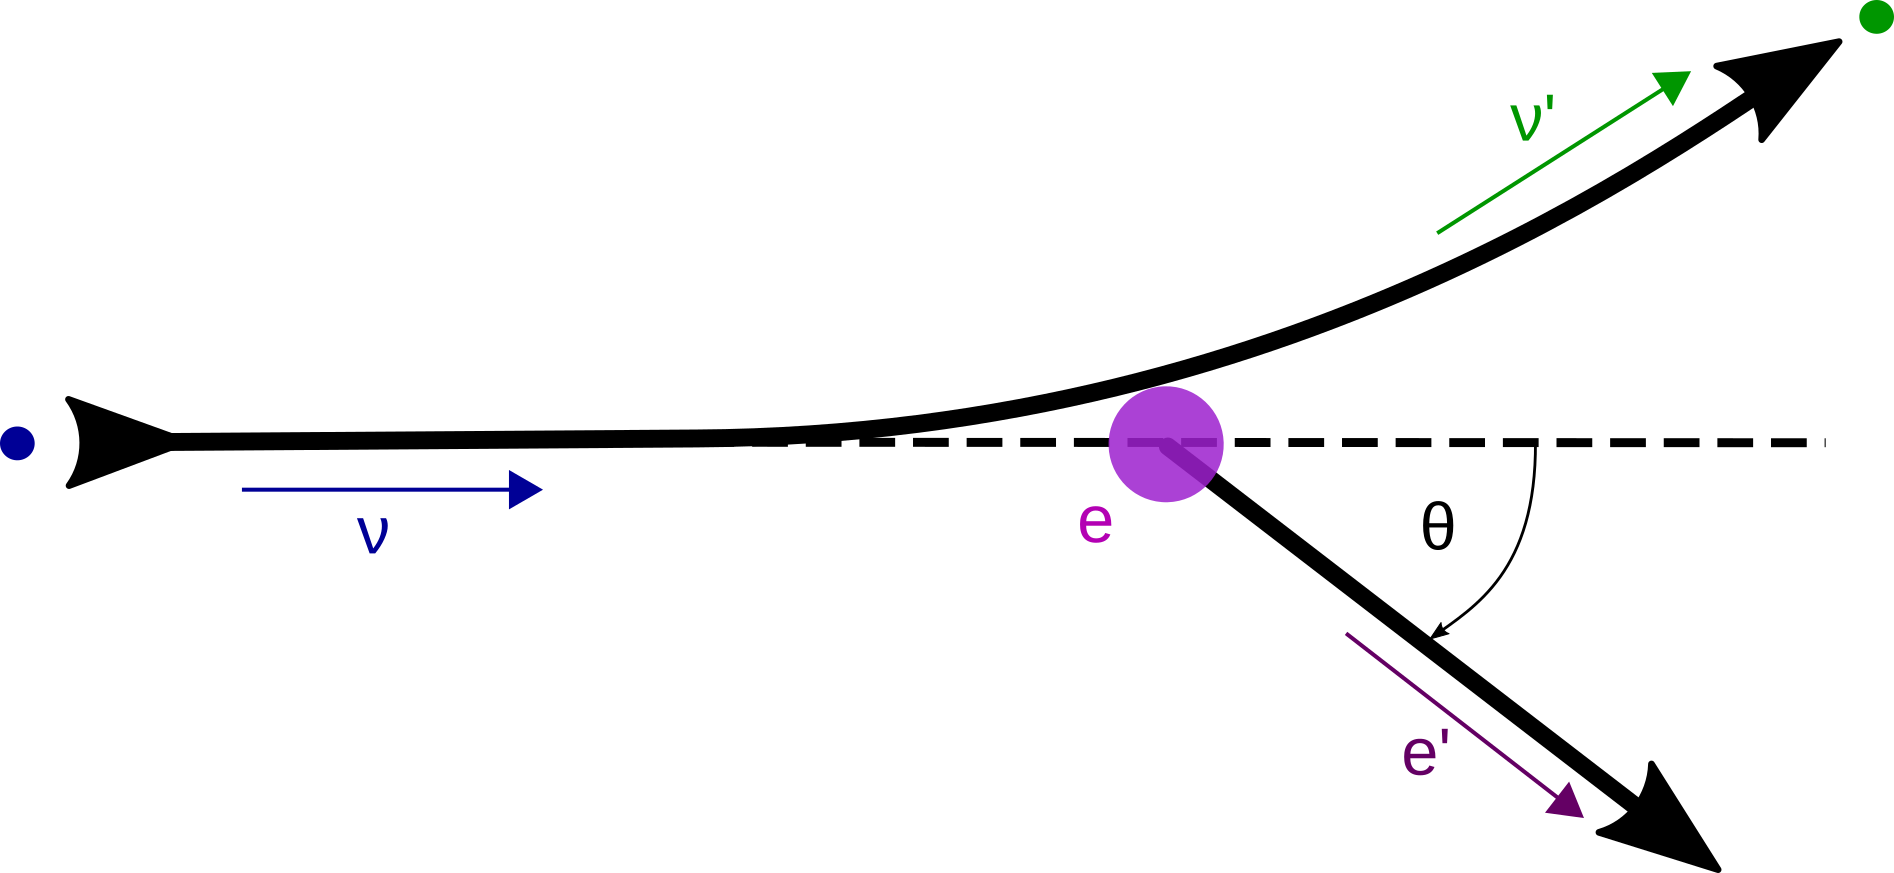
\includegraphics[width=0.55\linewidth]{Plots/NuMM/NuoneInteraction.png}
\caption{Neutrino-on-electron elastic scattering diagram}
\label{fig:NuoneDiagram}
\end{figure}

Since the \gls{nuone} interaction is governed by simple $2\rightarrow 2$ kinematics, it can be shown that
\begin{equation}
\left(P_{\nu}-P_{e^{\prime}}\right)^2=\left(P_{\nu^{\prime}}-P_e\right)^2,
\end{equation}
\begin{equation}
m_{\nu}^2+m_e^2-2E_{\nu}E_{e^{\prime}}+2E_{\nu}p_{e^{\prime}}\cos\theta=m_{\nu}^2+m_e^2-2E_{\nu^{\prime}}m_e.
\end{equation}
From the energy conservation
\begin{equation}
E_{\nu}+m_e=E_{\nu^{\prime}}+E_{e^{\prime}}=E_{\nu^{\prime}}+T_e+m_e\Rightarrow E_{\nu^{\prime}}=E_{\nu}-T_e
\end{equation}
it follows that
\begin{equation}
E_{\nu}p_{e^{\prime}}\cos\theta=E_{\nu}E_{e^{\prime}}-E_{\nu^{\prime}}m_e=E_{\nu}\left(T_e+m_e\right)-\left(E_{\nu}-T_e\right)m_e=T_e\left(E_{\nu}+m_e\right),
\end{equation}
\begin{equation}
\cos\theta=\frac{E_{\nu}+m_e}{E_{\nu}}\sqrt{\frac{T_e^2}{E_{e^{\prime}}^2-m_e^2}}=\frac{E_{\nu}+m_e}{E_{\nu}}\sqrt{\frac{T_e^2}{T_e^2+2T_em_e}}.
\end{equation}
And finally
\begin{equation}\label{eq:ThetaTRelation}
\cos\theta=\frac{E_{\nu}+m_e}{E_{\nu}}\sqrt{\frac{T_e}{T_e+2m_e}}.
\end{equation}
Which can be rearranged to get
\begin{equation}\label{eq:TThetaRelation}
T_e=\frac{2m_eE_\nu^2\cos^2\theta}{\left(E_\nu+m_e\right)^2-E_\nu^2\cos^2\theta}.
\end{equation}
The electron's kinetic energy is therefore constrained as
\begin{equation}
T_e\leq\frac{2E_{\nu}^2}{2E_{\nu}+m_e},
\end{equation}
which corresponds to the limit $\cos\theta\rightarrow 1$ when the recoil electron goes exactly forward in the incident neutrino direction, as depicted in Fig.~\ref{fig:TThetaDistribution}.

\begin{figure}[hbtp]
\centering
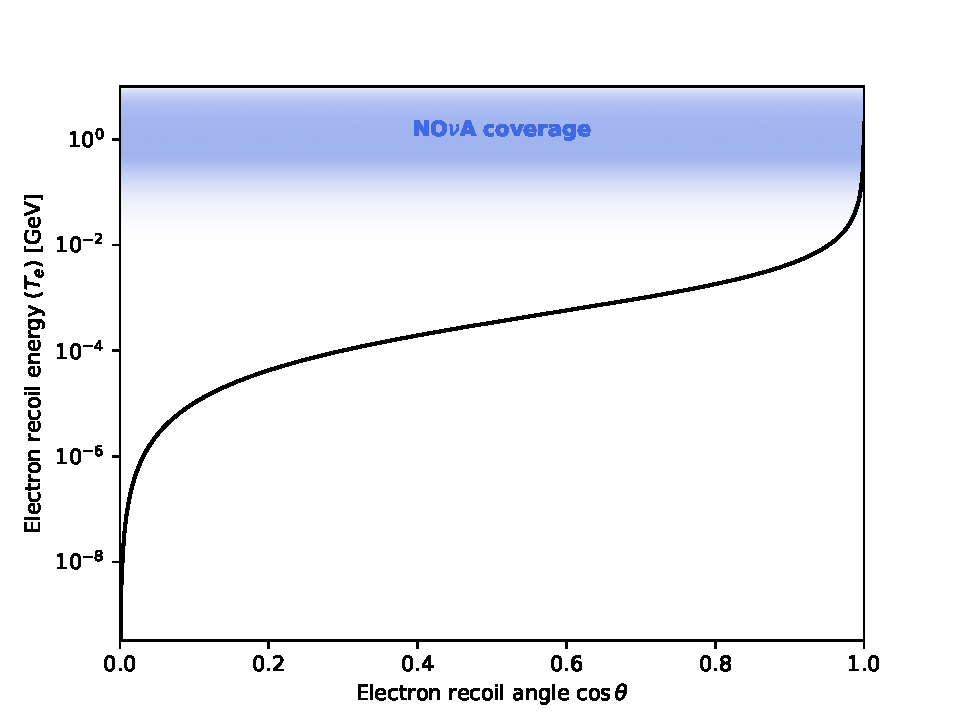
\includegraphics[width=.7\linewidth]{Plots/NuMM/KinematicsTOnTh.pdf}
\caption[Electron recoil energy versus recoil angle]{Relation between the recoil electron's kinetic energy and angle for the \acrshort{nuone} elastic scattering. The coverage of the \acrshort{NOvA} detectors for measuring the electron recoil energy is shown in blue. Only very forward electrons are therefore recorded in \acrshort{NOvA}.}
\label{fig:TThetaDistribution}
\end{figure}

Considering $E_{\nu}\sim\textsf{GeV}$, it is useful to approximate $\frac{m_e^2}{E_{\nu}^2}\rightarrow 0$. Additionally, considering only very small electron recoil angles, meaning $\theta^2\cong \left(1-\cos^2\theta\right)$, applied to Eq.~\ref{eq:ThetaTRelation} results in
\begin{equation}
T_e\theta^2\cong T_e\left(1-\left(\frac{E_\nu+m_e}{E_\nu}\right)^2\frac{T_e}{T_e+2m_e}\right)
=T_e\left(1-\left(1+\frac{2m_e}{E_\nu}\right)\frac{T_e}{T_e+2m_e}\right),
\end{equation}
therefore
\begin{equation}
T_e\theta^2\cong \frac{2m_eT_e}{T_e+2m_e}\left(1-\frac{T_e}{E_\nu}\right)=2m_e\left(\frac{1}{1+\frac{2m_e}{T_e}}\right)\left(1-\frac{T_e}{E_\nu}\right),
\end{equation}
and finally
\begin{equation}\label{eqTThetaSqExp}
T_e\theta^2\cong 2m_e\left(1-\frac{T_e}{E_{\nu}}\right)<2m_e.
\end{equation}

This is a strong limit that very clearly distinguishes the \gls{nuone} elastic scattering events from other similar interactions involving single electron (mainly the $\nu_e$\gls{CC} interactions).

\subsubsection{Neutrino magnetic moment cross section}
In the ultra-relativistic limit, the neutrino magnetic moment interaction flips the neutrino helicity, while the \gls{SM} weak interaction conserves it, which means it is possible to add the two contributions to the total \gls{nuone} cross section incoherently (without interference terms) \cite{nuElmagInt2015.pdf}:
\begin{equation}
\frac{d\sigma_{\gls{nuone}}}{dT_e}=\left(\frac{d\sigma_{\gls{nuone}}}{dT_e}\right)_{\textsf{SM}}+\left(\frac{d\sigma_{\gls{nuone}}}{dT_e}\right)_{\textsf{MAG}}.
\end{equation}

The \gls{SM} contribution can be expressed as \cite{FundamentalsOfNeutrinoPhysics.pdf, nuElmagInt2015.pdf}:
\begin{equation}\label{eq:NuMMSMCrossSection}
\left(\frac{d\sigma_{\gls{nuone}}}{dT_e}\right)_{\textsf{SM}}=\frac{2G_F^2m_e}{\pi}\left\lbrace g_1^2+g_2^2\left(1-\frac{T_e}{E_{\nu}}\right)^2-g_1 g_2\frac{m_eT_e}{E_{\nu}^2}\right\rbrace,
\end{equation}
where the coupling constants $g_1$ and $g_2$ differ between neutrino flavours and between neutrinos and antineutrinos. Their values are:
\begin{align}
g_1^{\nu_e}&=g_2^{\overline{\nu}_e}=\sin^2\theta_W+1/2,\hspace{2.5cm} g_2^{\nu_e}=g_1^{\overline{\nu}_e}=\sin^2\theta_W,\\
g_1^{\nu_{\mu,\tau}}&=g_2^{\overline{\nu}_{\mu,\tau}}=\sin^2\theta_W-1/2,\hspace{2.25cm} g_2^{\nu_{\mu,\tau}}=g_1^{\overline{\nu}_{\mu,\tau}}=\sin^2\theta_W,
\end{align}
where $\sin^2\theta_W\cong 0.23$.

The total \gls{SM} cross section, and therefore the number of \gls{SM} \gls{nuone} interactions, depends on the neutrino energy and the minimum measured electron recoil energy. However, in general the cross section for for $\nu_e$ is about $2.5$ times larger than for the $\overline{\nu}_e$, about $6$ times larger than for $\nu_{\mu/\tau}$ and about $7$ times larger than for $\overline{\nu}_{\mu/\tau}$.

The neutrino magnetic moment contribution is \cite{NeutrinoElmagFormFactors1989.pdf, nuElmagInt2015.pdf}:
\begin{equation}\label{eq:NuMMMMCrossSection}
\left(\frac{d\sigma_{\gls{nuone}}}{dT_e}\right)_{\textsf{MAG}}=\frac{\pi\alpha^2}{m_e^2}\left(\frac{1}{T_e}-\frac{1}{E_{\nu}}\right)\left(\frac{\mu_{\nu_l}}{\mu_B}\right)^2,
\end{equation}
where $\alpha$ is the fine structure constant and $\mu_{\nu_l}$ is the effective magnetic moment of $\nu_l$. The total cross section now only depends on the neutrino energy and on the effective magnetic moment, but is the same for neutrinos and antineutrinos.

The comparison of the \gls{SM} and the neutrino magnetic moment differential cross sections is shown in Fig.\ref{fig:NuMMCrossSectionComparison}. Whereas the \gls{SM} cross section is approximately uniform for $T_e\rightarrow 0$, the neutrino magnetic moment cross section rises to infinity. However, this reach is limited by the experimental capabilities of detecting electrons with very low energies. The (possible) \gls{NOvA} coverage is shown with a shaded blue region, with current capability reaching $T_e=\unit[0.5]{GeV}$. Future analyses might extend this reach to lower $T_e$, with the lowest possible detectable electron recoil energy \mbox{$T_{e,min}\approx\unit[0.01]{GeV},$} as discussed in Sec.~\ref{sec:NOvADetectors}.

\begin{figure}[hbtp]
\centering
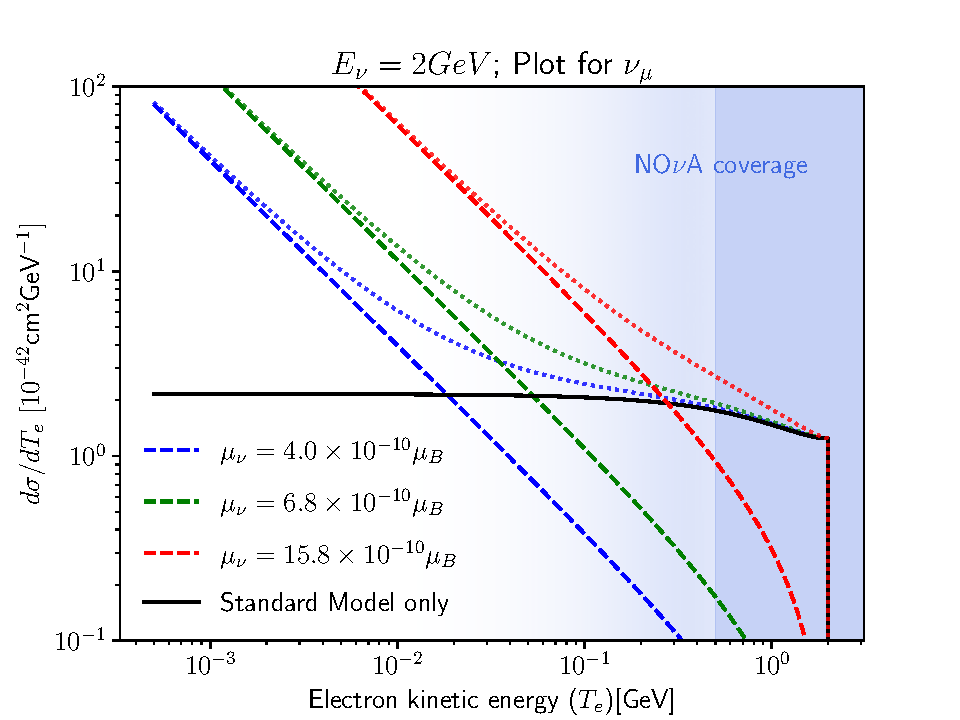
\includegraphics[width=.9\textwidth]{Plots/NuMM/dSdTNumuMMCompAltLim.pdf}
\caption[Comparison of the neutrino magnetic moment and the Standard Model cross sections]{Comparison of the neutrino magnetic moment (coloured) and the \acrshort{SM} (black) cross sections for the \acrshort{nuone} elastic scattering. Different colours depict different values of the neutrino magnetic moment, with red corresponding to the previous \acrshort{NOvA} measurement, green the LSND result, and blue a possible ultimate \acrshort{NOvA} sensitivity, as discussed in the introduction to this chapter. Dashed lines are the individual cross sections and dotted lines are the added total cross section with the standard model contribution. \acrshort{NOvA} coverage of electron recoil energies is shown in shaded blue.}
\label{fig:NuMMCrossSectionComparison}
\end{figure}

Calculating the ratio of the neutrino magnetic moment and the \gls{SM} cross sections, as shown in Fig.~\ref{fig:NuMMCrossSectionRatios}, can serve as a proxy to estimate the number of neutrino magnetic moment events in relation to the predicted number of \gls{SM} events, if the $E_\nu$ and $T_e$ are known. Additionally, comparing the ratio of the total cross sections can reveal the expected total number of neutrino magnetic moment events as a function of the predicted number of \gls{SM} events. Considering $E_\nu=\unit[2]{GeV}$, $\mu_\nu=6.8\times10^{-10}\mu_B$ (current best limit for $\nu_\mu$ from LSND), and integrating differential cross sections for $\nu_\mu$ in Eq.~\ref{eq:NuMMSMCrossSection} and \ref{eq:NuMMMMCrossSection} from $T_{e,min}$ to $T_{e,max}\rightarrow\unit[2]{GeV}$ results in
\begin{equation}
\frac{\sigma_{\textsf{MAG}}}{\sigma_{\textsf{SM}}}\approx
\begin{cases}
0.035\hspace*{1.5cm} T_{e,min}=\unit[0.5]{GeV},\\
0.14\hspace*{1.7cm}  T_{e,min}=\unit[0.01]{GeV}.
\end{cases}
\end{equation}
Therefore, at the current \gls{NOvA} detection capabilities, there are about $0.035$ times as many neutrino magnetic moment \gls{nuone} events than \gls{SM} ones. This can be compared with the expected statistical uncertainty on the \gls{SM} background, which in the case of Poisson distributed events is the square root of the number of predicted events. Consequently, it is possible to assess the minimal number of \gls{SM} \gls{nuone} events necessary for the magnetic moment signal to be detected above the \gls{SM} background (without considering systematic uncertainties) as
\begin{equation}
N_{\gls{SM}}>1/0.035^2 \approx 816.
\end{equation}
However, this approximation is calculated only for one value of $E_\nu$, but can be used to assess the sensitivity of the experiment.

\begin{figure}[hbtp]
\centering
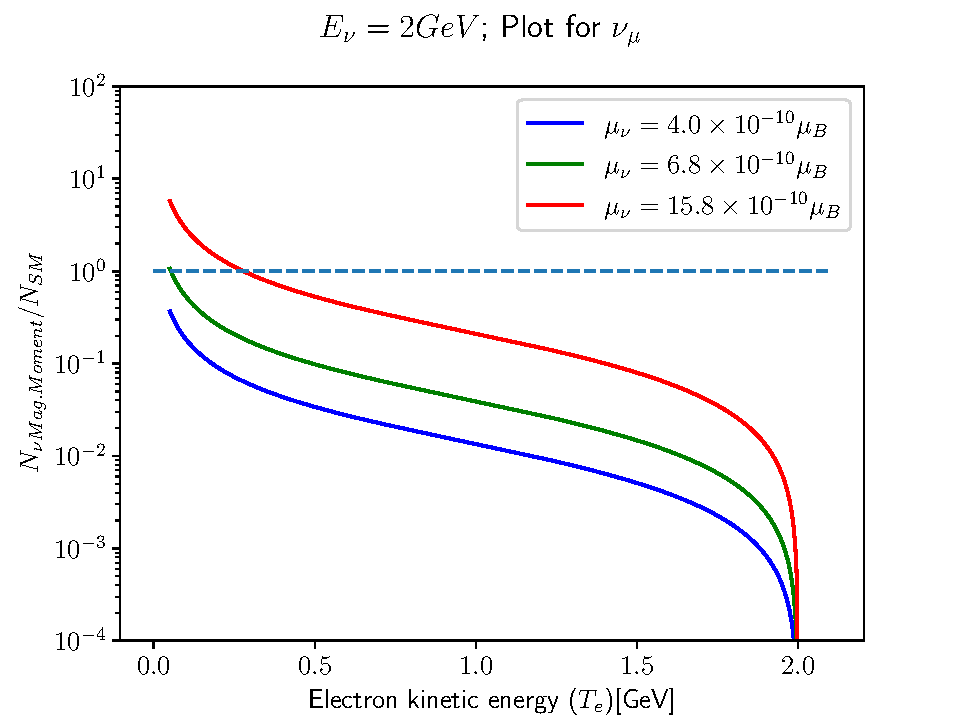
\includegraphics[width=.9\textwidth]{Plots/NuMM/RatioNumuMMCompLinX.pdf}
\caption[Ratio of the neutrino magnetic moment and the Standard Model cross sections]{Ratio of the neutrino magnetic moment cross section to the \acrshort{SM} cross section for the \acrshort{nuone} elastic scattering of $\unit[2]{GeV}$ $\nu_\mu$. Different colours depict different effective muon neutrino magnetic moment values, with red corresponding to the previous \acrshort{NOvA} measurement, green the LSND result, and blue a possible ultimate \acrshort{NOvA} sensitivity, as discussed in the introduction to this chapter.}
\label{fig:NuMMCrossSectionRatios}
\end{figure}

As can be seen in Fig.~\ref{fig:NuMMCrossSectionComparison} and Fig.~\ref{fig:NuMMCrossSectionRatios}, the magnetic moment contribution exceeds the \gls{SM} contribution for low enough $T_e$. This can be approximated as \cite{nuElmagInt2015.pdf}:
\begin{equation}
T_e\lesssim\frac{\pi^2\alpha^2}{G_F^2m_e^3}\left(\frac{\mu_{\nu}}{\mu_B}\right)^2\simeq 2.9\times 10^{19}\left(\frac{\mu_{\nu}}{\mu_B}\right)^2\left[\textsf{MeV}\right],
\end{equation}
which does not depend on the neutrino energy. Therefore, experiments sensitive to lower energetic electrons are significantly more sensitive to the neutrino magnetic moment.
\fi
%%%%%%%%%%%%%%%%%%%%%%%%%%%%%%%%%%%%%%%%%%%%%%%%%%%%%%%%%%%%%%%%%%%%%
%%%                       ANALYSIS OVERVIEW                       %%%
%%%%%%%%%%%%%%%%%%%%%%%%%%%%%%%%%%%%%%%%%%%%%%%%%%%%%%%%%%%%%%%%%%%%%
\section{Analysis overview}\label{sec:NuMMAnalysisOverview}

Our analysis strategy for measuring the effective muon neutrino magnetic moment in the \gls{NOvA} \gls{ND} is based on comparing the total number of reconstructed and selected events in data with the prediction. The predicted events consist of the signal, which depends on the size of the effective muon neutrino magnetic moment, and of the background, which corresponds to the \gls{SM}-only (null) hypothesis without any neutrino magnetic moment. We define the signal as true \gls{nuone} elastic scattering interactions, created with the use of the neutrino magnetic moment cross section instead of the \gls{SM} cross section, as described in Sec.~\ref{sec:MeasuringNuMM}. Additionally, the signal events are required to have their true interaction vertex contained within the \gls{ND} to exclude events originating from outside of the detector.

The data used in this analysis were collected from the start of \gls{NOvA} \gls{ND} data taking on the August 22$^{\textsf{nd}}$, 2014, until February 3$^{\textsf{rd}}$, 2021. This is the \gls{ND} data that were used in the latest \gls{NOvA} neutrino oscillations result \cite{NOvAResults2021.pdf}, with an additional year. Although more data have been collected since February 2021, they are still being processed and are not available at the time of writing this thesis. The total exposure of the data sample is approximately $13.8\times10^{20}$~\gls{POT}. This exposure is used throughout this chapter to scale the predicted distributions and number of events.

This analysis uses the standard \gls{NOvA} simulation and reconstruction tools, as were discussed in Sec.~\ref{sec:NOvASimulation} and \ref{sec:NOvAReconstruction}. The simulation was created with approximately four times larger statistics than the data to limit statistical uncertainties from simulation. The total exposure for the simulation is approximately $55.4\times10^{20}$~\gls{POT}. For the systematic uncertainty studies only a portion of this full sample is used, specifically $19.3\times10^{20}$~\gls{POT}.

%Analysis weights - PPFX and cross section
Corrections for known limitations in the simulation are applied in the form of analysis weights applied to each event based on how it is affected by specific variations in the simulation. This includes the corrections for the neutrino beam prediction based on the external measurements used by the \gls{PPFX} (Sec.~\ref{sec:NOvASimulation}), and, for the non-\gls{nuone} background only, also the internal and external measurements that constrain the neutrino interaction prediction inside GENIE.

%Radiative correction weight
The cross section corrections are not applied to the \gls{nuone} events, as they are assumed to be known precisely from theory. However, the GENIE \gls{MC} simulation only considers tree-level \gls{SM} \gls{nuone} interactions \cite{NOVA-doc-56383}, as described in Sec.~\ref{sec:MeasuringNuMM}, and doesn't account for any higher order terms, which are described by radiative corrections.
Radiative corrections can be expressed by two adjustments to the tree-level \gls{SM} \gls{nuone} cross section \cite{MinervaNuoneFluxConstraint2019.pdf}. First, the values of the weak coupling constants are changed as \cite{NuoneRadCorrConstants2013.pdf}
\begin{equation}
g_1^{\nu_e}\rightarrow 0.7276,\; \; g_1^{\nu_\mu}\rightarrow -0.2730,\; \;  g_2\rightarrow 0.2334.
\end{equation}
Second, there are additional terms added to the cross section equation. Considering only one-loop corrections, the full \gls{nuone} cross section can be expressed as\footnote{There is technically a third correction term $X_3$ by the $g_1g_2$ term, which is however negligible for $E_\nu\sim\unit{GeV}$.} \cite{NuoneRadCorrEquation1984.pdf}
\begin{equation}
\left(\frac{d\sigma_{\gls{nuone}}}{dy}\right)_{\textsf{Rad. Corr.}}=
\frac{G_F^2s}{\pi}\left\lbrace
g_1^2\left(1+\frac{\alpha}{\pi}X_1\right)+
g_2^2\left(1-y\right)^2\left(1+\frac{\alpha}{\pi}X_2\right)-
g_1 g_2\frac{m_ey}{E_{\nu}}\right\rbrace,
\end{equation}
where
\begin{equation}
y=\frac{T_e+E_\gamma}{E_\nu},
\end{equation}
$s=2E_\nu m_e+m_e^2$ is the Mandelstam variable,
\begin{equation}
X_1=-\frac{2}{3}\log\left(\frac{2yE_\nu}{m_e}\right)+\frac{y^2}{24}-\frac{5y}{12}-\frac{\pi^2}{6}+\frac{23}{72}
\end{equation}
and
\begin{equation}
X_2=-\frac{2}{3}\left(1-y\right)^2\log\left(\frac{2yE_\nu}{m_e}\right)-\frac{y^2}{18}-\frac{\pi^2}{6}\left(1-y\right)^2-\frac{2y}{9}+\frac{23}{72}.
\end{equation}

In practice, radiative corrections can be implemented as a weight, where each true \gls{nuone} event is weighted by a ratio
\begin{equation}
\textsf{weight}_{\textsf{Rad. Corr.}}\left(E_\nu,T_e\right) = \left.\left(\frac{d\sigma_{\gls{nuone}}}{dy}\right)_{\textsf{Rad. Corr.}}\; \middle/\; \left(\frac{d\sigma_{\gls{nuone}}}{dy}\right)_{\textsf{GENIE 3}}\right.;
\end{equation}

%MINERvA paper \cite{MinervaNuoneFluxConstraint2019.pdf}: At tree level, the neutrino-electron scattering cross section is given by... (basically same as I have in the theory) corrected for updated electroweak couplings, CLL and CLR [17] and one-loop electroweak radiative corrections as calculated in Ref. [18]. One deficiency of the calculation of Ref. [18] is that it does not contain the term in the one-loop cross section proportional to CLL CLR. This deficiency is corrected in a recent calculation [38], and that result is given below. However, as illustrated in Eq. (A1) this term also contains an additional power of m/Enu compared to the terms proportional to C2 LL and C2 LR, and the entire term is therefore negligible at the few-GeV neutrino energies of the MINERvA experiment.
%[17] is https://www.sciencedirect.com/science/article/pii/S0146641013000239?via%3Dihub \cite{NuoneRadCorrConstants2013.pdf}
%[18] is https://www.sciencedirect.com/science/article/pii/0550321384902931?via%3Dihub \cite{NuoneRadCorrEquation1984.pdf}

%[ND group's technote] In GENIE, the cross section of the nuone elastic scattering signal is calculated at the tree level. To improve the precision of the simulated nuone elastic scattering cross section, we performed radiative corrections to the GENIE nuone elastic scattering as shown in Appendix A. The precision of the simulated nuone elastic scattering cross section is improved by tuning CLL and CLR to one-loop values obtained from global fits to electroweak data 14 and 2. The radiative correction also includes additional low-energy terms in the expression of differential cross section of nuone elastic scattering. In comparison, the neutrino interactions in the NOvA detector are simulated using the GENIE neutrino event generator, where the Weinberg Angle is 0.501716712132. After radiative corrections, the total number of nuone elastic scattering increases  0.83\% from the standard GENIE MC.

%Magnetic moment as a weight 
Analogically to the radiative correction weight, it is possible to create a neutrino magnetic moment weight as a ratio between the neutrino magnetic moment and the \gls{SM} differential cross sections for the \gls{nuone} interactions. This can then serve to predict the number of \gls{nuone} events created by the neutrino magnetic moment interaction (which make up the signal), without the need for an additional simulation. This is possible thanks to the theoretically very well understood properties of the \gls{nuone} interaction, as described in Sec.~\ref{sec:MeasuringNuMM}. Therefore, the signal sample is created from the true \gls{nuone} sample, with the magnetic moment weight applied. The weight has a form:
\begin{equation}
\textsf{weight}_{\nu \textsf{Mag. Mom.}}\left(E_\nu,T_e\right) = \left.\left(\frac{d\sigma_{\gls{nuone}}}{dy}\right)_{\nu \textsf{Mag. Mom.}}\; \middle/\; \left(\frac{d\sigma_{\gls{nuone}}}{dy}\right)_{\textsf{GENIE 3}}\right.,
\end{equation}
where
\begin{equation}
\left(\frac{d\sigma_{\gls{nuone}}}{dy}\right)_{\nu \textsf{Mag. Mom.}} = E_\nu \left(\frac{d\sigma_{\gls{nuone}}}{dT_e}\right)_{\nu \textsf{Mag. Mom.}}.
\end{equation}

%Enhanced nuone sample
Due to the relatively low cross section of the \gls{nuone} interaction, the nominal simulation sample contains very few \gls{nuone} events, which could result in a significant statistical uncertainty from simulation. To avoid this, we created a \gls{nuone}-enhanced simulation sample, which is mainly made up of \gls{nuone} events with a total exposure of $1.72\times10^{24}$~\gls{POT}. There are a few non-\gls{nuone} background events overlaid on top of the \gls{nuone} events to properly account for the possible reconstruction effects of the pileup of neutrino interactions in a single spill \cite{NOVA-doc-56383}, since in the real detector, the hits from the true \gls{nuone} interaction can be clustered together into another interaction, or additional hits can be clustered together into the \gls{nuone} event. To save up on unnecessary disk space and processing usage, the enhanced \gls{nuone} sample does not include any cross section related parameters and variables, as the \gls{nuone} interaction is assumed to be known exactly from theory. Therefore, we do not apply cross section weights or account for cross section systematic uncertainties for \gls{nuone} events.

%[ND group's technote] Because the cross section of the nuone elastic scattering is very low (approx. 1/2000 of the total charged-current cross section), the statistics of nuone elastic scattering is not enough in the inclusive sample. In order to optimize the signal selection criteria, we made a sample with only nuone elastic scattering events in the detector. The size of this nuone signal MC is 1.48E23 POT. However the pile-up of neutrino interactions in one spill impacts on the hit clustering in reconstruction, either hits from the nuone elastic scattering can be clustered to other interactions or extra hits can be clustered to the nuone elastic scattering.

% enhanced nueccmec
The cross section tuning procedure in \gls{NOvA} (Sec.~\ref{sec:NOvASimulation}) applies large weights to \gls{MEC} events in some parts of the parameter space. However, after the full event selection (Sec.~\ref{sec:NuMMEventSelection}) only a small number of \gls{MEC} events remain in the detector. This was shown to be an issue especially for the $\nu_e$\gls{CC} \gls{MEC} events  \cite{NOVA-doc-56383}. Applying large tuning corrections to a small number of events results in large statistical fluctuations. To avoid this, we created another special sample with enhanced number of $\nu_e$\gls{CC} \gls{MEC} events, following the same procedure as for the \gls{nuone}-enhanced sample, with an exposure of $1.99\times10^{24}$~\gls{POT}.

%Created by Yiwen Xiao \cite{NOVA-doc-56383} to tackle the low statistics of the $\nu_e$CC MEC background events and subsequently large and unphysical cross section weights. Correct POT is 1.99e+24 (filematched). There are limitations of the sample in the q3-q0 parameter space.

%[ND group's technote] After implementing GSF Xsec weights, the shape of background after selection shows multiple spikes from nue CC events.  Since the number of nue CC MEC events remained in the final sample is small, events with very large weight can distort the distribution of nue CC MEC events. In order to mitigate the effect for nue CC MEC events in the signal and sideband region (ETh2 < 0.04 GeV Rad2), a special nue CC MEC sample is produced with enlarged statistics. The nue CC MEC events after all selection in Production 5.1 MC are replaced by the nue CC MEC events in the special sample in the sections of DATA analysis and Systematic Uncertainty.

\iffalse
NOvAReweight reference: J. Wolcott, “NOvARwgt software.” https://github.com/novaexperiment/NOvARwgt-public.
[ND group's technote] The cross-section weight is a combination of different weights applied to various processes. The major effects of this weight are
\begin{itemize}
\item  Adjust the axial mass (MA) for CCQE cross section to $\unit[1.04]{GeV/c^2}$ based on the error-weighted mean of updated ANL, BNL, and FNAL experiments.
\item Applies the empirical MEC weight determined from the cross section tuning fit.
\item Reduces non-resonant single pion production by 50\%.
\item Applies RPA suppression that models nuclear screen effects at low values Q2 to QE and RES interactions.
\item Reduces GENIE predicted DIS events with $W>\unit[1.7]{GeV}$ by 10\%.
\end{itemize}
\fi


A summary of the simulation samples and analysis weights for the four different types of signal and background components is shown in Tab.~\ref{tab:NuMMSamplesAndWeightsOverview}. In the following chapter, the $\nu_e$\gls{CC} \gls{MEC} background is added into the `Other background' sample, even though it is created from a separate simulation.

\begin{table}[!ht]
\centering
\caption{Overview of the simulation samples and analysis weight used for the different signal and background components.}
\def\arraystretch{1.4}
\begin{tabular}{l@{\hskip 1cm}l@{\hskip 1cm}l}
Signal type            & Sample               & Weight\\\hline
Signal                 & Enhanced \gls{nuone} & Flux \& $\nu$ Mag. Moment\\
\gls{nuone} background & Enhanced \gls{nuone} & Flux \& Rad. Corr.\\
$\nu_e$\gls{CC} \gls{MEC} background & Enhanced $\nu_e$\gls{CC} \gls{MEC} & Flux \& Cross Sec.\\
Other background       & Nominal \gls{ND}     & Flux \& Cross Sec.
\end{tabular}
\label{tab:NuMMSamplesAndWeightsOverview}
\end{table}

%%%%%%%%%%%%%%%%%%%%%%%%%%%%%%%%%%%%%%%%%%%%%%%%%%%%%%%%%%%%%%%%%%%%%
%%%                         EVENT SELECTION                       %%%
%%%%%%%%%%%%%%%%%%%%%%%%%%%%%%%%%%%%%%%%%%%%%%%%%%%%%%%%%%%%%%%%%%%%%
\section{Event selection}\label{sec:NuMMEventSelection}
%Introduction:
We are searching for \gls{nuone} elastic scattering events, characterised by a single very forward going electron shower, specifically focusing on low electron recoil energies. The main backgrounds for our analysis come from $\nu_e$\gls{CC} interactions, which produce an electron with additional activity, and interactions that produce $\pi^0$, which decays into two photons producing electromagnetic showers, where each can look similar to the \gls{nuone} signal. Additionally, there are $\nu_\mu$\gls{CC} interactions, which are generally easy to distinguish from our signal, however, their very high abundance in the \gls{NOvA} \gls{ND} makes them a dominant background nevertheless.

I explain the motivation behind each cut of the event selection and discuss their effect on the neutrino magnetic moment events below. I also consider possible improvements to the event selection for a future (re-)analysis.

The strategy for event selection is as follows. First, I remove events that failed reconstruction or data collection, described in Sec.~\ref{sec:NuMMEventSelSpillCuts} and \ref{sec:NuMMEventSelRecoQC}. Then, I apply pre-selection cuts that remove obvious background (Sec.~\ref{sec:NuMMEventSelectionPresel}), while limiting the reduction of the signal efficiency to about $\unit[0.25]{\%}$. Following this, I apply the containment cuts (Sec.~\ref{sec:NuMMEventSelFidCont}) that remove events that are either not fully contained within the detector, or events that originate from outside of the detector, such as rock muons. Afterwards, I perform a cut-based \gls{MVA} on a selection of variables useful for distinguishing the signal from the background, discussed in Sec.~\ref{sec:NuMMEventSelTMVA}, and evaluate their combined performance on the signal selection. I choose the cut values that result in the best statistical significance, based on a chosen \gls{FOM}. Given that we are searching for a very limited number of signal events on top of a large background, I chose a simple statistics-only \gls{FOM}
\begin{equation}\label{eq:NuMMFOM}
\textsf{\gls{FOM}} = \frac{\textsf{Signal}}{\sqrt{\textsf{Background}}}.
\end{equation}

The summary of the cut values for the event selection of neutrino magnetic moment signal is presented in Tab.~\ref{tab:EventSelectionSummary}, showing the label for the event selection variable, its description and the cut value chosen. After the full event selection, the predicted number of signal events for $\mu_\nu=10^{-9}\mu_B$ is $56.80$ and the total number of background events under the \gls{SM} hypothesis is $700.33$.

\begin{table}[!hb]
\centering
\caption[Event selection summary]{Summary of the variables and their cut values for the event selection of neutrino magnetic moment signal. Showing the category of the event selection variable, its label, description and the cut value chosen.}
\begin{tabular}{|m{2mm} m{0.175\textwidth} m{0.54\textwidth} m{0.145\textwidth}|}\hline
& \textbf{Label} & \textbf{Description} & \textbf{Cut} \\\hline
\parbox[t]{2mm}{\multirow{5}{*}{\rotatebox[origin=c]{90}{\textbf{Reco Qual.}}}} &
\textbf{Valid Vtx} & Valid reconstructed vertex & $>0$\\
& \textbf{N$^o$ Prongs} & Number of reconstructed prongs & $>0$\\
& \textbf{Hits / Plane} & Number of hits per plane & $<6$\\
& \textbf{Low $E_{Shower}$} & Low cut on calorimetric energy of the most energetic shower & $>\unit[0.5]{GeV}$\\\hline
\parbox[t]{2mm}{\multirow{6}{*}{\rotatebox[origin=c]{90}{\textbf{Pre-selection}}}} &
\textbf{N$^o$~Hits Loose} & Preliminary cut on the total number of hits for all prongs in a slice & $<280$\\
& \textbf{Prong Length} & Length of the longest prong & $<\unit[640]{cm}$\\
& \textbf{$E\theta^2$ Loose} & Preliminary cut on the product of the calorimetric energy and angle squared of the leading shower & $<0.064$ $\unit{GeV\times rad^2}$\\\hline
\parbox[t]{2mm}{\multirow{6}{*}{\rotatebox[origin=c]{90}{\textbf{Fiducial}}}} &
\multirow{6}{*}{\textbf{Vertex}} & \multirow{2}{*}{x position} & $>\unit[-177]{cm}$\\
& & & $<\unit[177]{cm}$\\
& & \multirow{2}{*}{y position} & $>\unit[-177]{cm}$\\
& & & $<\unit[177]{cm}$\\
& & \multirow{2}{*}{z position} & $\unit[>50]{cm}$\\
& & & $<\unit[1170]{cm}$\\\hline
\parbox[t]{2mm}{\multirow{6}{*}{\rotatebox[origin=c]{90}{\textbf{Containment}}}} &
\multirow{6}{*}{\textbf{Prong}} & Minimum hit position in x & $>\unit[-177]{cm}$\\
& & Maximum hit position in x & $<\unit[177]{cm}$\\
& & Minimum hit position in y & $>\unit[-185]{cm}$\\
& & Maximum hit position in y & $<\unit[177]{cm}$\\
& & Minimum hit position in z & $>\unit[55]{cm}$\\
& & Maximum hit position in z & $<\unit[1270]{cm}$\\\hline
\parbox[t]{2mm}{\multirow{9}{*}{\rotatebox[origin=c]{90}{\textbf{Selection}}}} &
\textbf{$E_{Shower}/E_{Tot}$} & Fraction of energy contained in the most energetic shower & $>0.91$\\
& \textbf{N$^o$ Hits} & Total number of hits for all prongs in a slice & $<116$\\
& \textbf{High $E_{Shower}$} & Calorimetric energy of the most energetic shower & $<\unit[1.4]{GeV}$\\
& \textbf{\acrshort{nuoneID}} & \gls{CVN}-based \gls{nuone} identifier & $>0.65$\\
& \textbf{\acrshort{EPi0ID}} & \gls{CVN}-based \gls{nuone} and $\pi^0$ identifier & $>0.63$\\
& \textbf{$E\theta^2$} & Product of the calorimetric energy and angle squared of the leading shower & $<0.0048$ $\unit{GeV\times rad^2}$\\\hline
\end{tabular}
\label{tab:EventSelectionSummary}
\end{table}

\subsection{Data collection quality}\label{sec:NuMMEventSelSpillCuts}
To ensure good data quality, we apply the following criteria to data (not applied to simulation) \cite{NOvA-doc-59876}. A cut on the time of each spill relative to other spills and on the exposure of each spill, where every spill is required to have at least $2\time10^{12}$ \gls{POT}. Additionally, the current in the focusing horn is required to be within $\unit[-202]{kA}<I_{Horn}<\unit[-196.4]{kA}$, the position of the beam to be within $\pm\unit[2]{cm}$ in both x and y axis, and that the width of the beam to be within $0.57$ and $\unit[1.58]{cm}$. Furthermore, incomplete events, or events with issues in one or more \glspl{DCM} are removed.

\subsection{Reconstruction quality}\label{sec:NuMMEventSelRecoQC}
As described in Sec.~\ref{sec:NOvAReconstruction}, electrons are reconstructed by slicing, followed by vertexing, then clustering into prongs. To identify electrons we require a valid reconstructed vertex and at least one reconstructed prong. Even though electrons only consist of a single shower, we don't reject events with more than one prong in a slice, as the reconstruction can wrongly assign noise hits as a separate prong. These false secondary prongs can be removed later in the event selection.

Figure~\ref{fig:NuMMCutsVertexIsValid} and Tab.~\ref{tab:CutflowTableBasicRecoQC} show that about $\unit[68]{\%}$ of signal events do not have a valid reconstructed vertex. This is due to the concentration of signal events at very low electron recoil energies, which results in events that can consist of a small number of hits, or even a single hit. As can be seen in the bottom plot in Fig.~\ref{fig:NuMMCutsVertexIsValid}, events with small true electron recoil energies have much smaller vertex reconstruction efficiency than the higher energetic electrons. However, ongoing work is improving the vertex reconstruction in the \gls{NOvA} detectors with a use of \gls{ML} instead of the currently used Hough transform combined with Elastic Arms \cite{NOvA-doc-61190}. Improving \gls{NOvA} vertex reconstruction at low energies can enhance our event selection in the future.

\begin{figure}[hbtp]
\centering
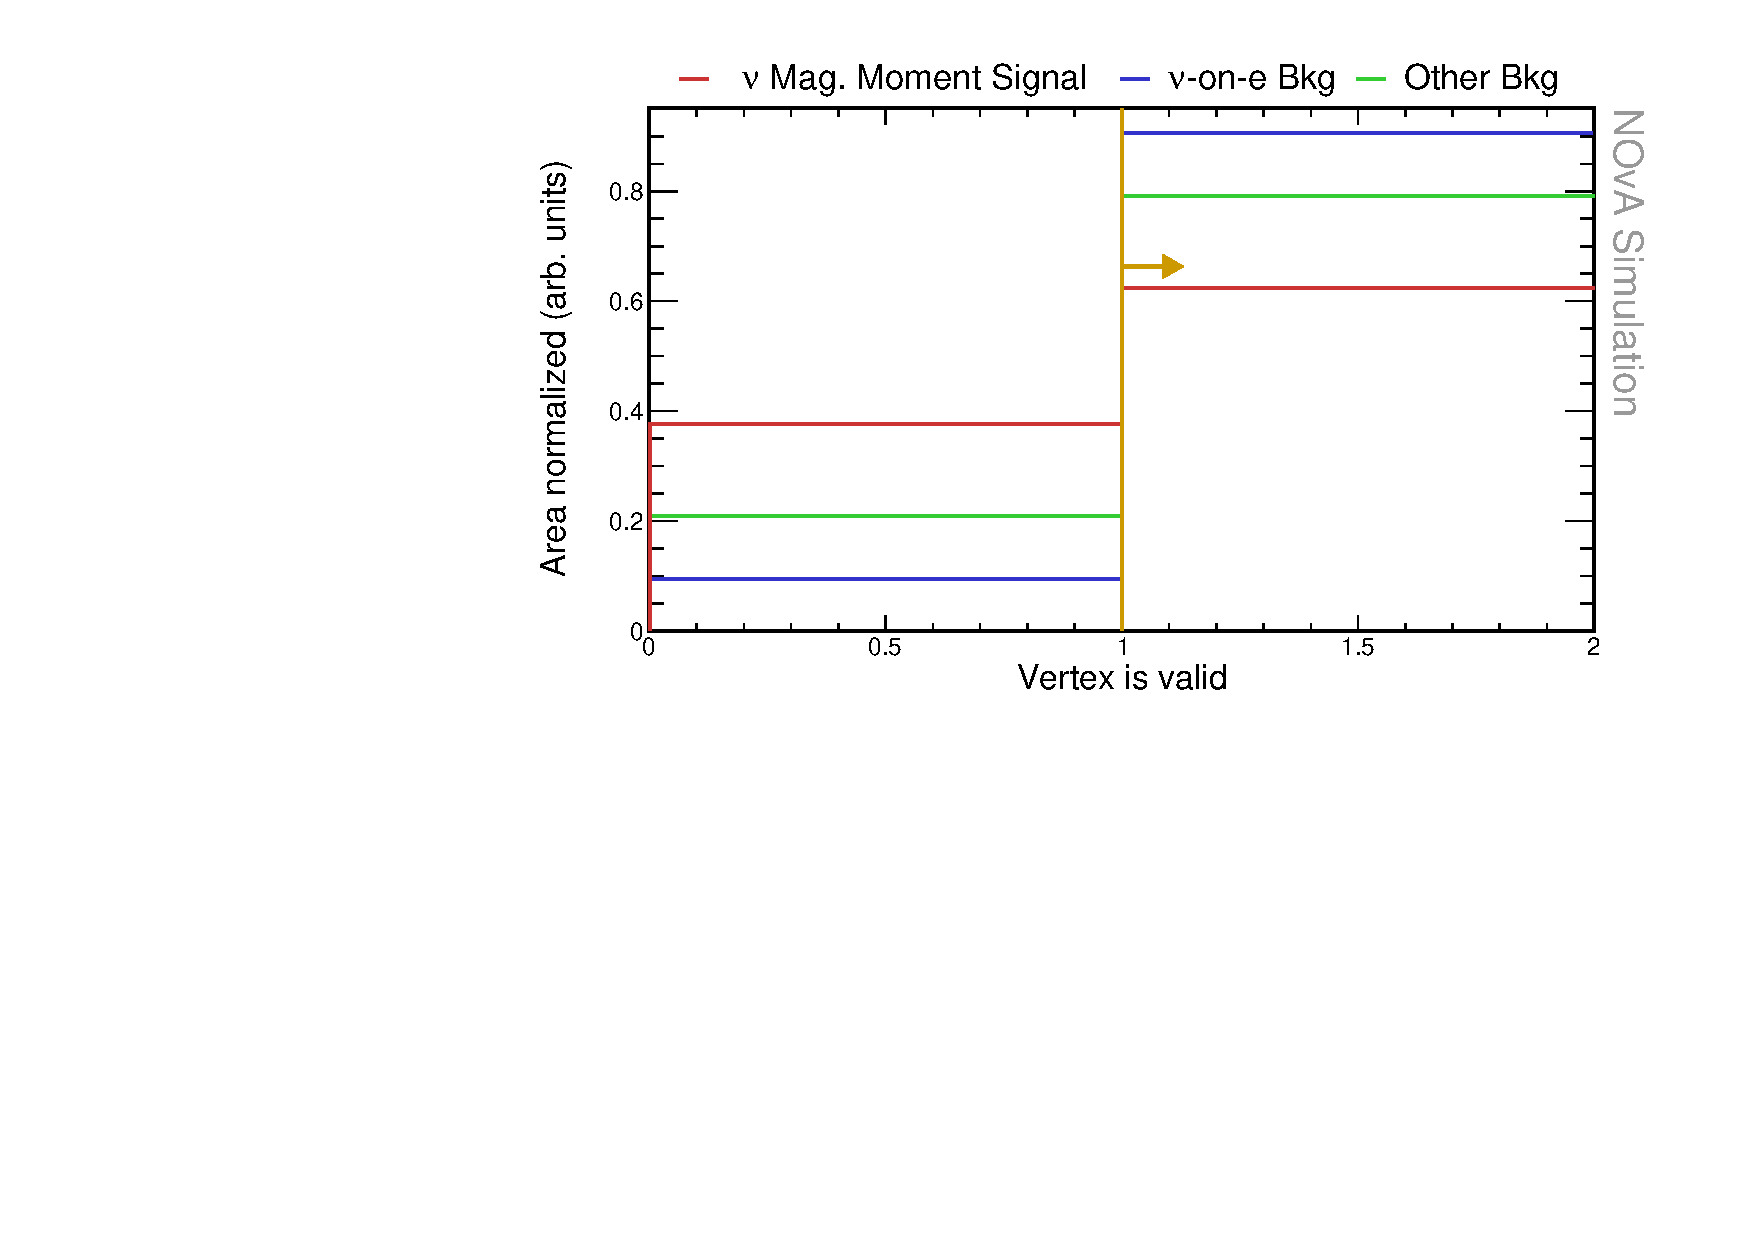
\includegraphics[width=.9\textwidth]{Plots/NuMMEventSelection/N1Cut_vtxIsValid.pdf}
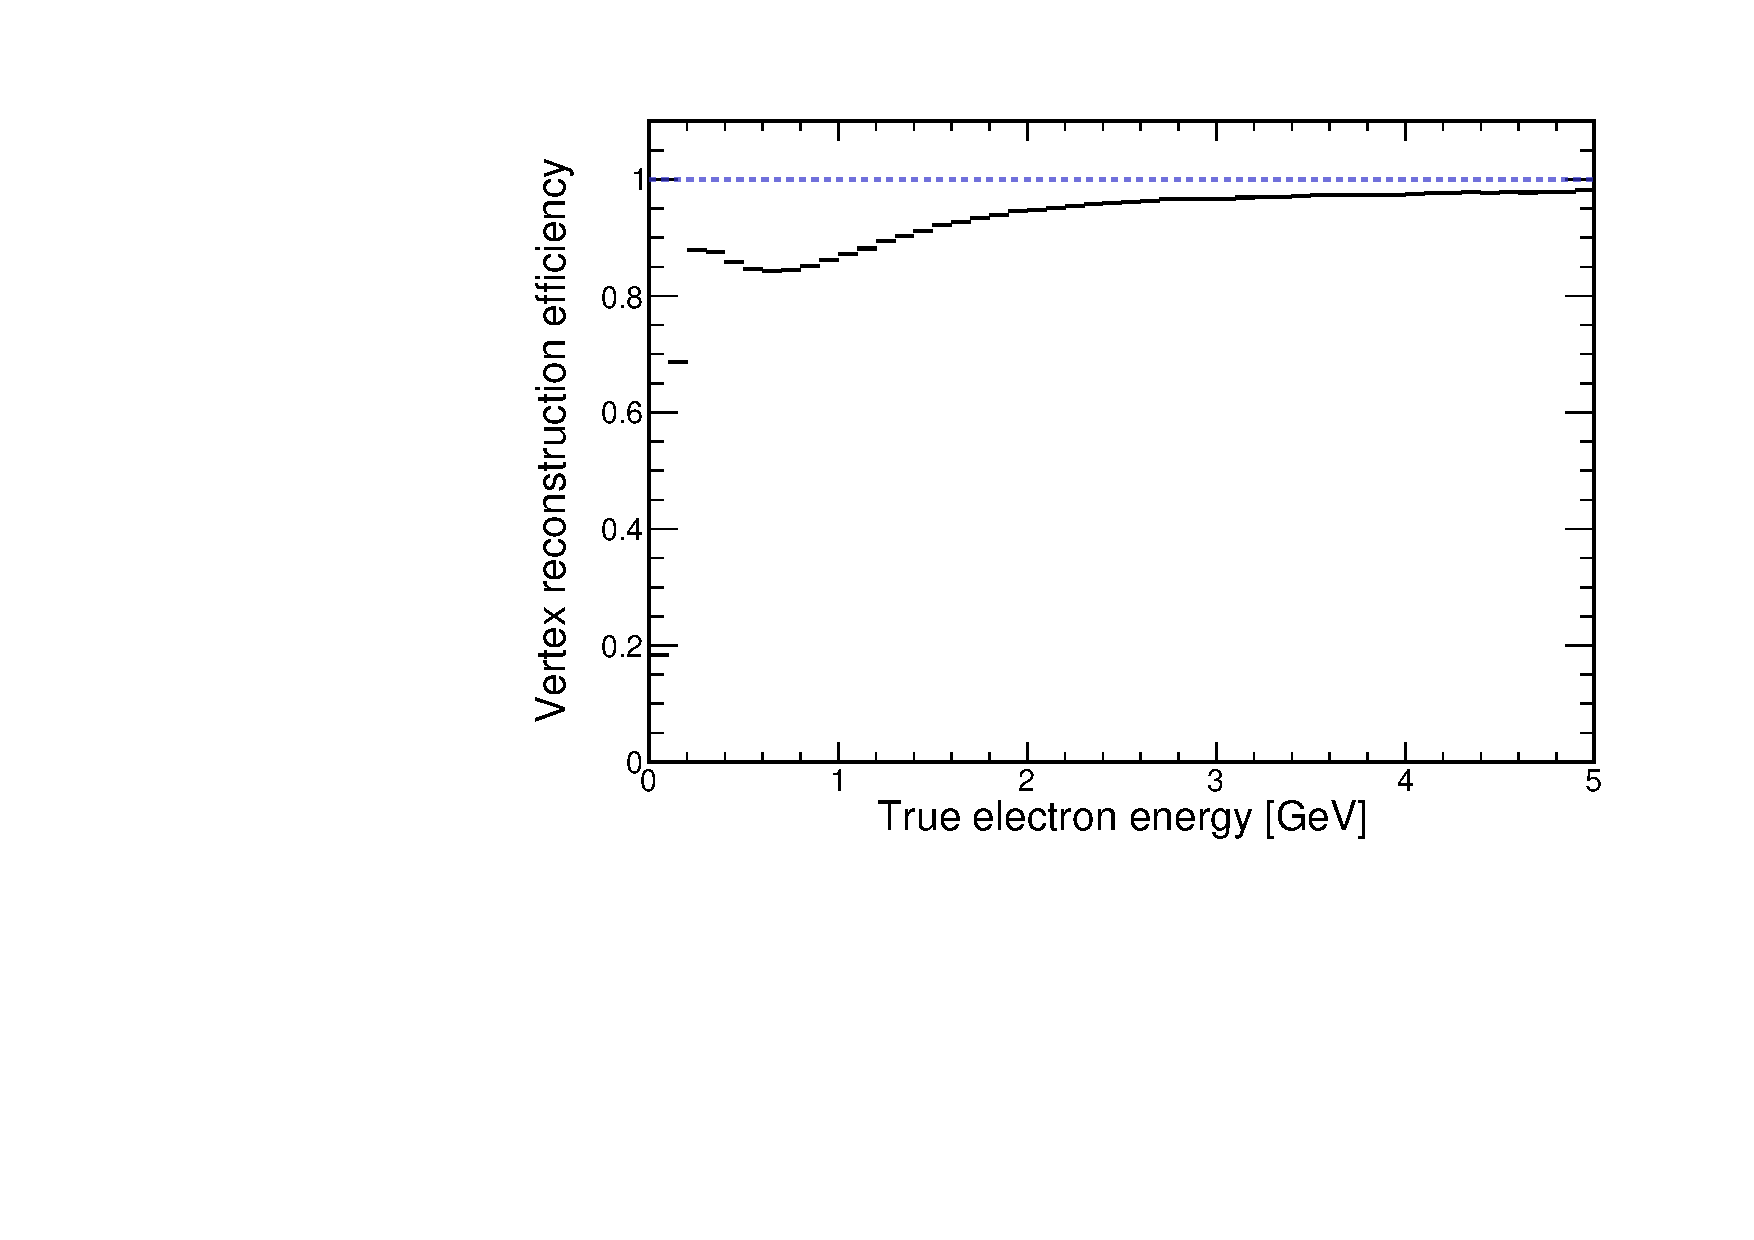
\includegraphics[width=.9\textwidth]{Plots/NuMMEventSelection/VtxIsValidNuMM.pdf}
\caption[Vertex reconstruction quality cut]{Top: Relative comparison of the signal (red), \acrshort{nuone} background (blue), and other background (green) events for the vertex reconstruction quality selection. Each histogram is area-normalised and the first bin corresponds to events without a valid vertex and second bin to events with correctly reconstructed vertex. The yellow line indicates the chosen cut value, where all events have to have a valid reconstructed vertex. Bottom: profile histogram of the `vertex is valid' variable as a function of the true electron energy for the true signal events, showing the significant drop in vertex reconstruction efficiency at low electron recoil energies. No selection was applied prior to making these plots.}
\label{fig:NuMMCutsVertexIsValid}
\end{figure}

Additionally, we limit the number of hits per plane to $<6$. This is to remove the so-called `\gls{FEB} flashers', which are caused by such a high energy deposit in one cell, that it affects all the other channels on the same \gls{APD} \cite{NOvA-doc-37668}. The cut value was chosen so that it removes approximately $\unit[0.25]{\%}$ signal events, which is the same criterion as is used for the pre-selection cuts described below. Relative comparisons between signal and background for the number of prongs and the number of hits per plane are shown in Fig.~\ref{fig:NuMMCutsRecoQuality}.

%In pre-selection we also include a cut on the time difference between the mean times of the "current" slice and of the slice closest in time, which should be $>25\ \unit{ns}$. This ensures that ... \todo{This is to remove slicing failures that split the two gamma from a $\pi^0$ into two slices that resemble electron signal. Should we remove them now though?}.

%[nueXSec ana, docdb:37668] One additional detector issues is the presence of "FEB Flashers" within reconstructed slices. FEB flashers are caused by high  energy deposits in one cell, which induces a sagged baseline in all other channels on the same APD. When the baseline is restored, fake hits are triggered on the whole APD.

\begin{figure}[hbtp]
\centering
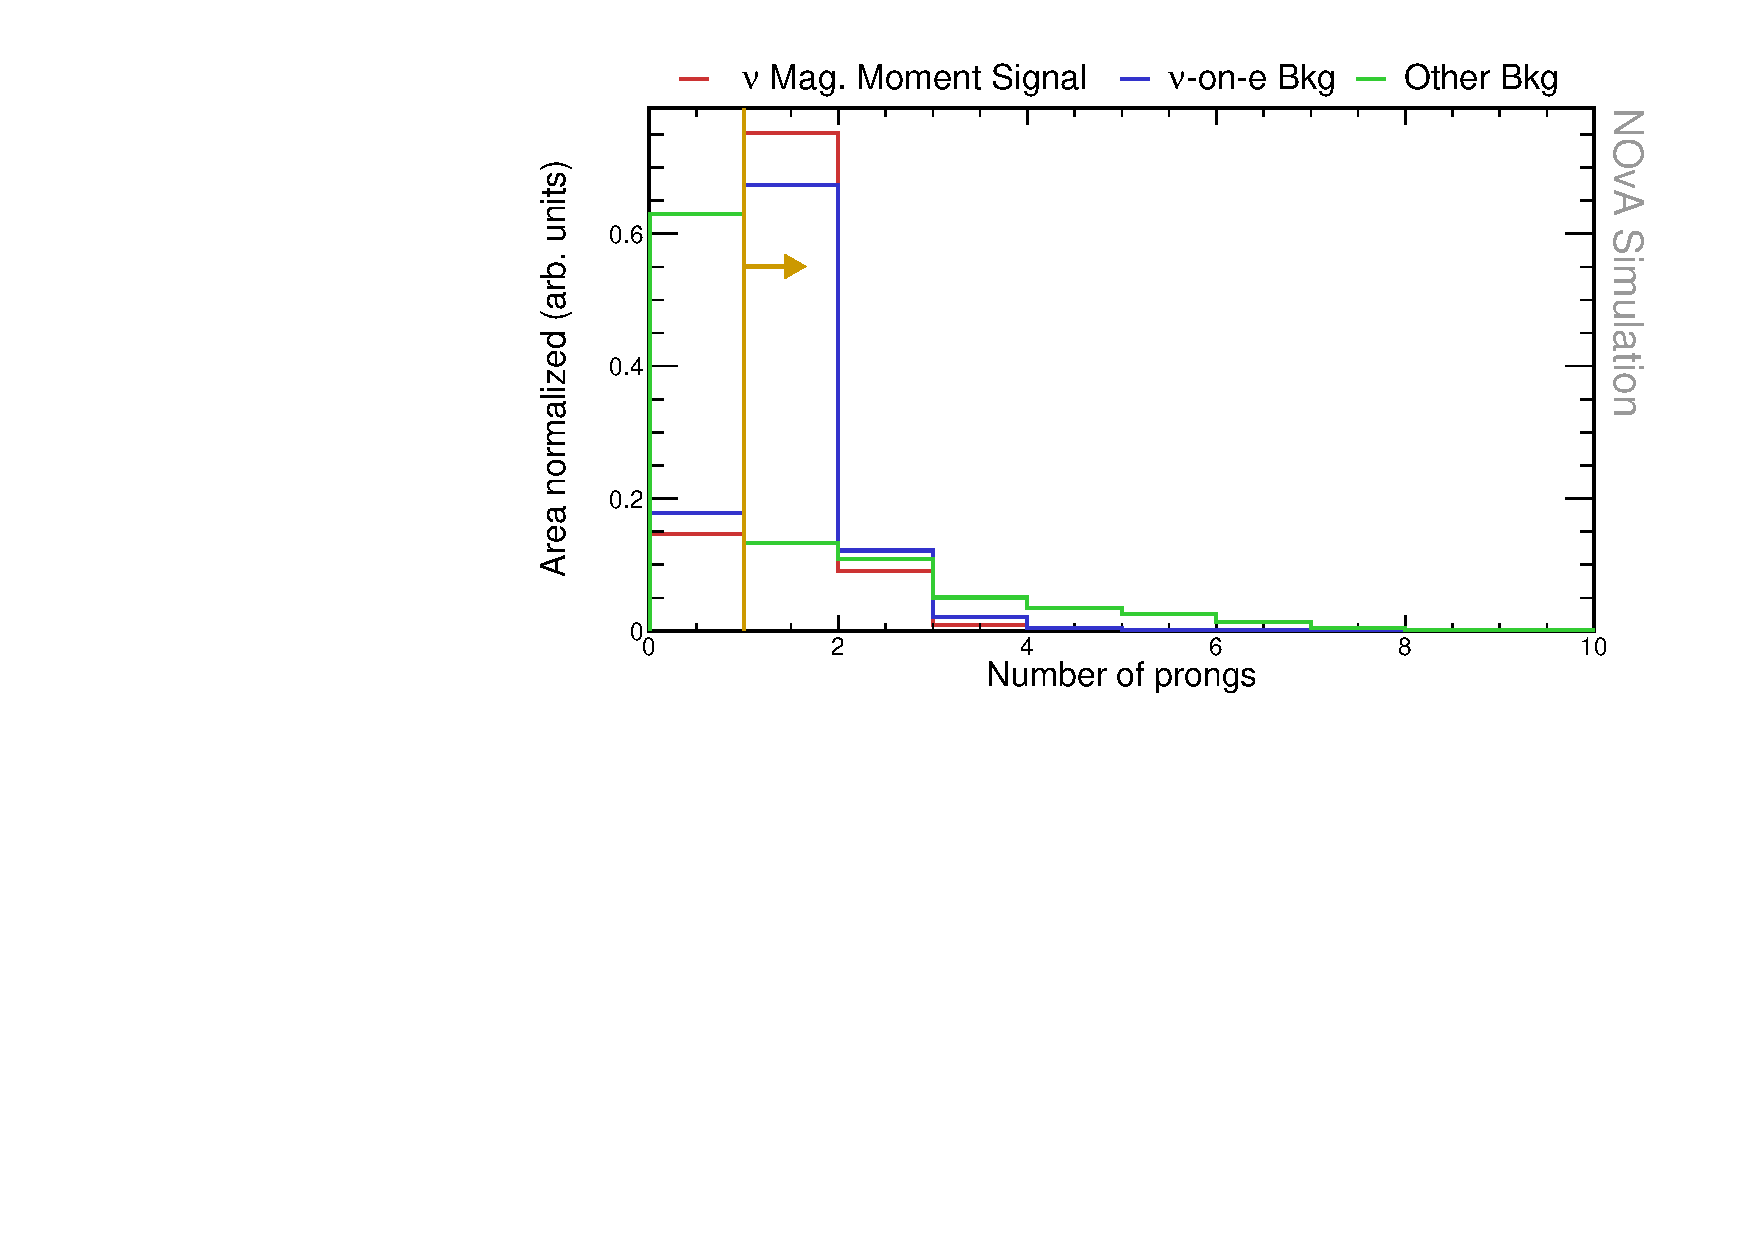
\includegraphics[width=.9\textwidth]{Plots/NuMMEventSelection/N1Cut_NPng.pdf}
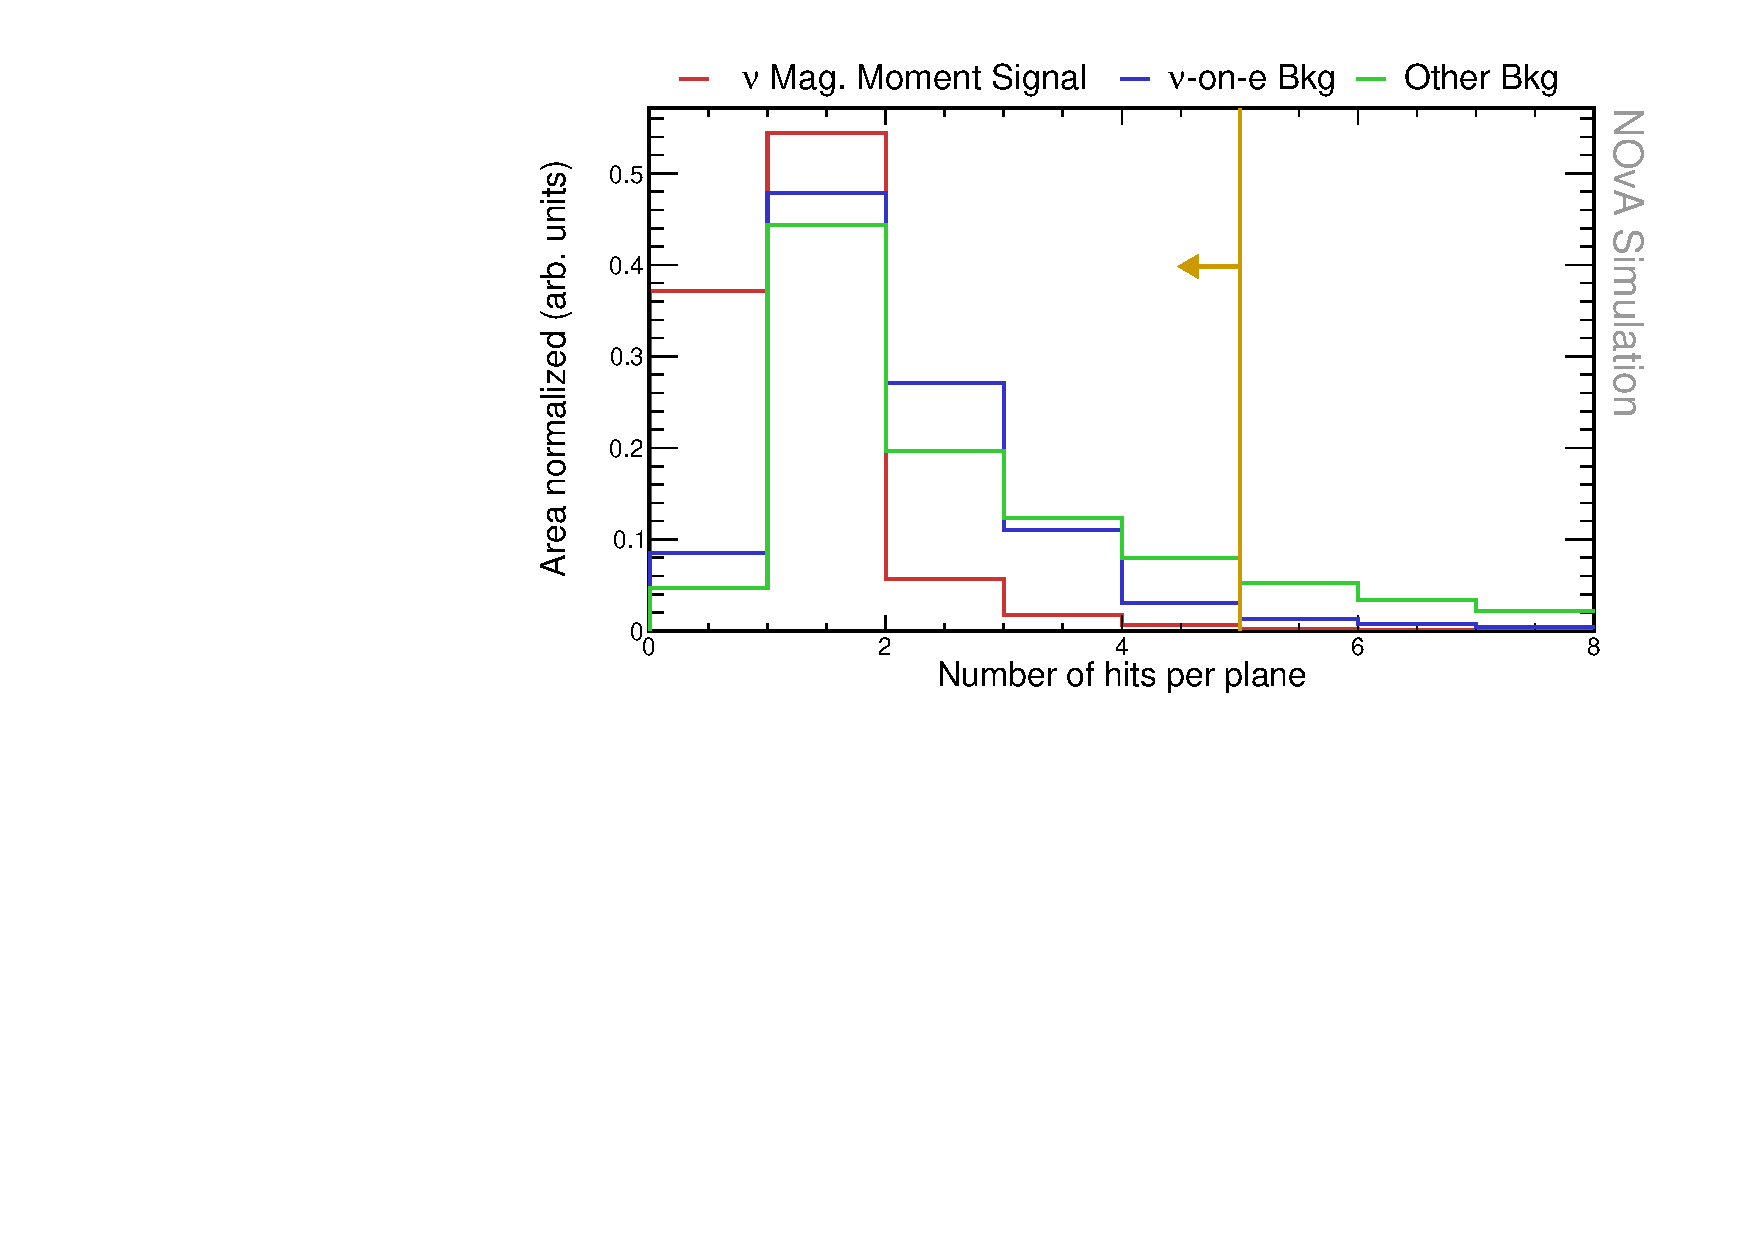
\includegraphics[width=.9\textwidth]{Plots/NuMMEventSelection/N1Cut_NHitsPPlane.pdf}
\caption[Prong and hits reconstruction quality cuts]{Relative comparison of signal (red), \acrshort{nuone} background (blue), and other background (green) events in the number of prongs (top) and the number of hits per plane (bottom) distributions. Events in both plots are required to have a valid reconstructed vertex and in the bottom plot also at least one reconstructed prong. Yellow lines indicate the cut values for the shown variables, with arrows pointing towards the preserved events. All histograms are area-normalised.}
\label{fig:NuMMCutsRecoQuality}
\end{figure}

%%% Low CalE
Furthermore, the reconstructed calorimetric energy of the primary shower is required to be $E_{cal} > \unit[0.5]{GeV}$ as shown in Fig.~\ref{fig:NuMMCutsLowCalE}. This is primarily due to the limitations of the currently used \gls{CVN}-based \gls{nuone} identifiers described in Sec.~\ref{sec:NuMMEventSelTMVA}, which were developed and validated for \gls{nuone} events with energies above this limit, to avoid the large background at low energies. However, due to the nature of the neutrino magnetic moment signal, which is concentrated at low electron recoil energies, this cut also removes a majority of our signal events, specifically $\unit[66.8]{\%}$. This large reduction severely impacts the significance of our measurement. On the other hand, it also marks potentially the most impactful improvement available in a future re-analysis. There are other event identifying algorithms available in \gls{NOvA} that could be explored for \gls{nuone} events to leverage the low energy sample. Additionally, it is possible to develop a purpose-built \gls{nuone} identifier focusing on low electron recoil energies.

\begin{figure}[hbtp]
\centering
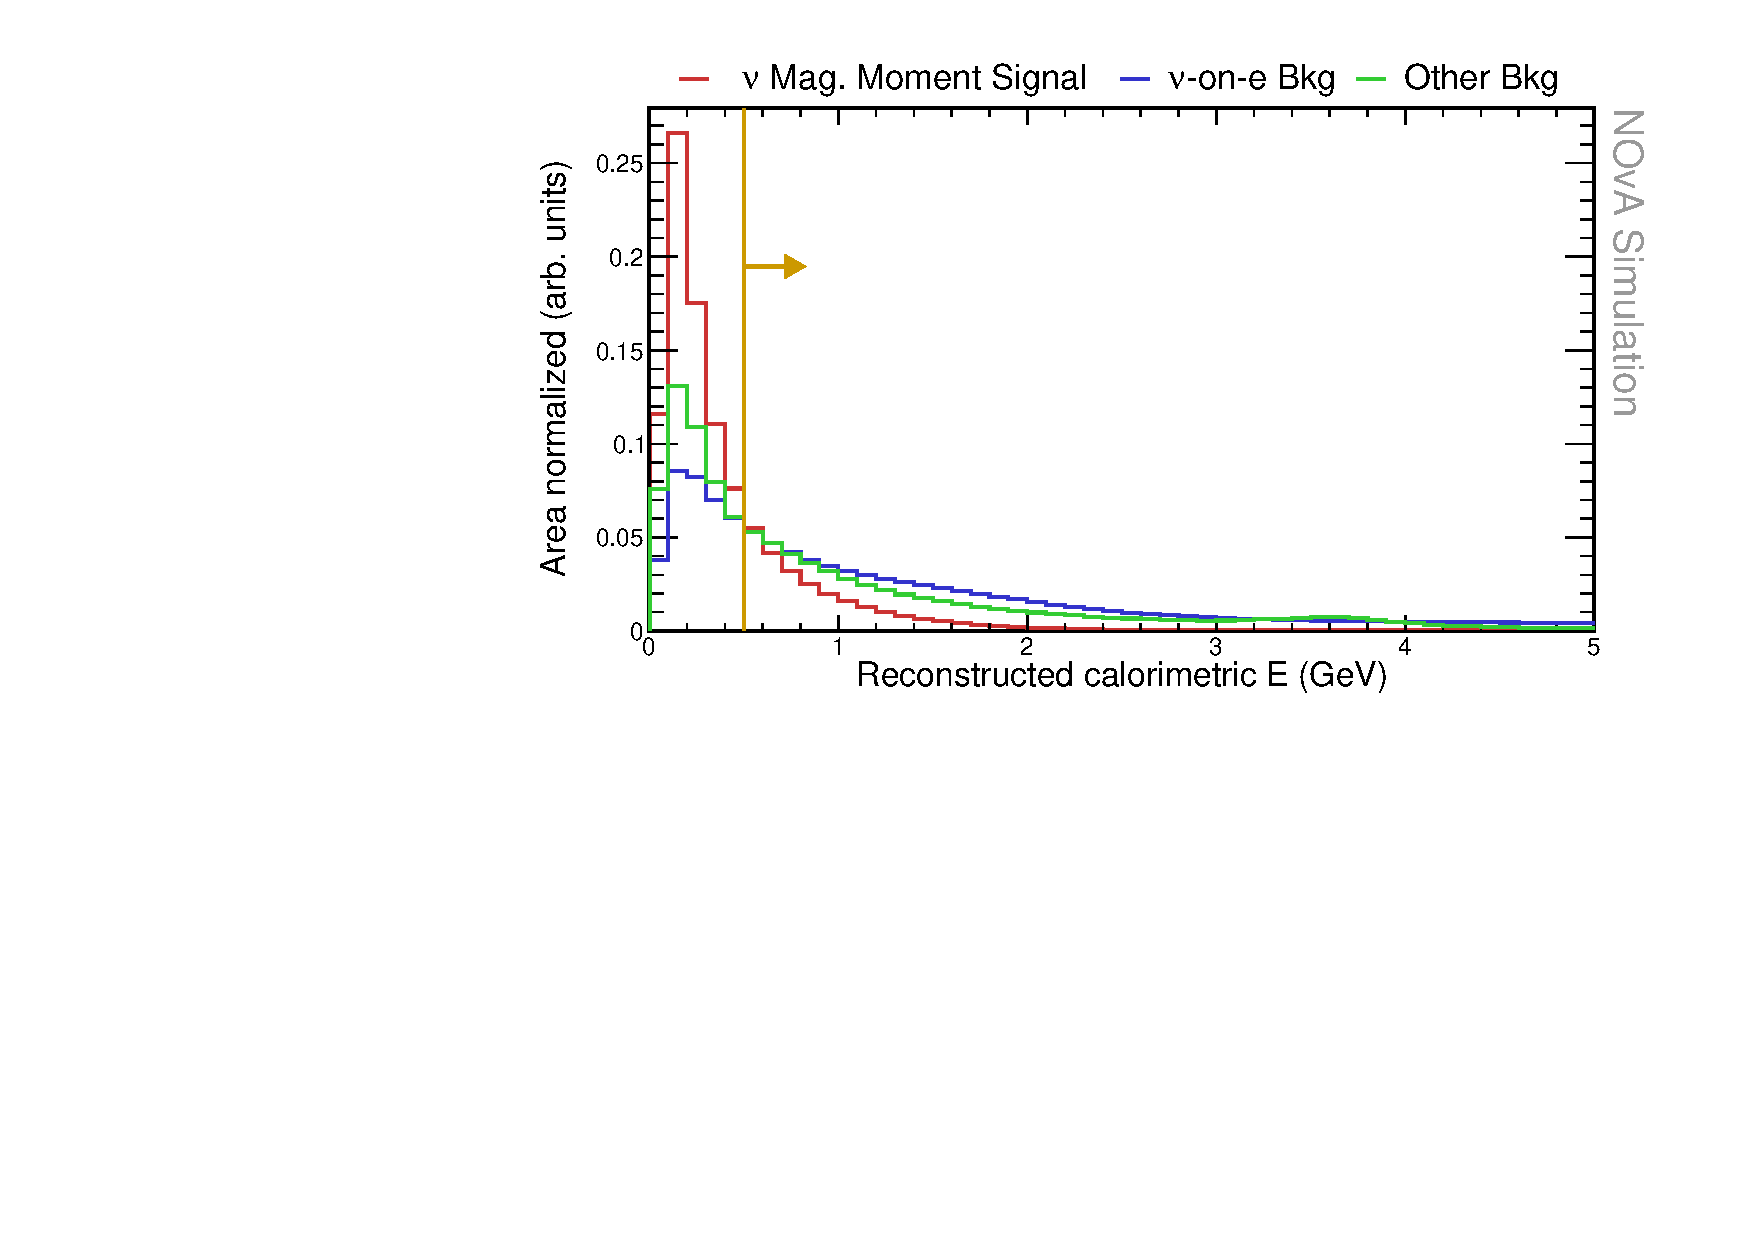
\includegraphics[width=.9\textwidth]{Plots/NuMMEventSelection/N1Cut_calELow.pdf}
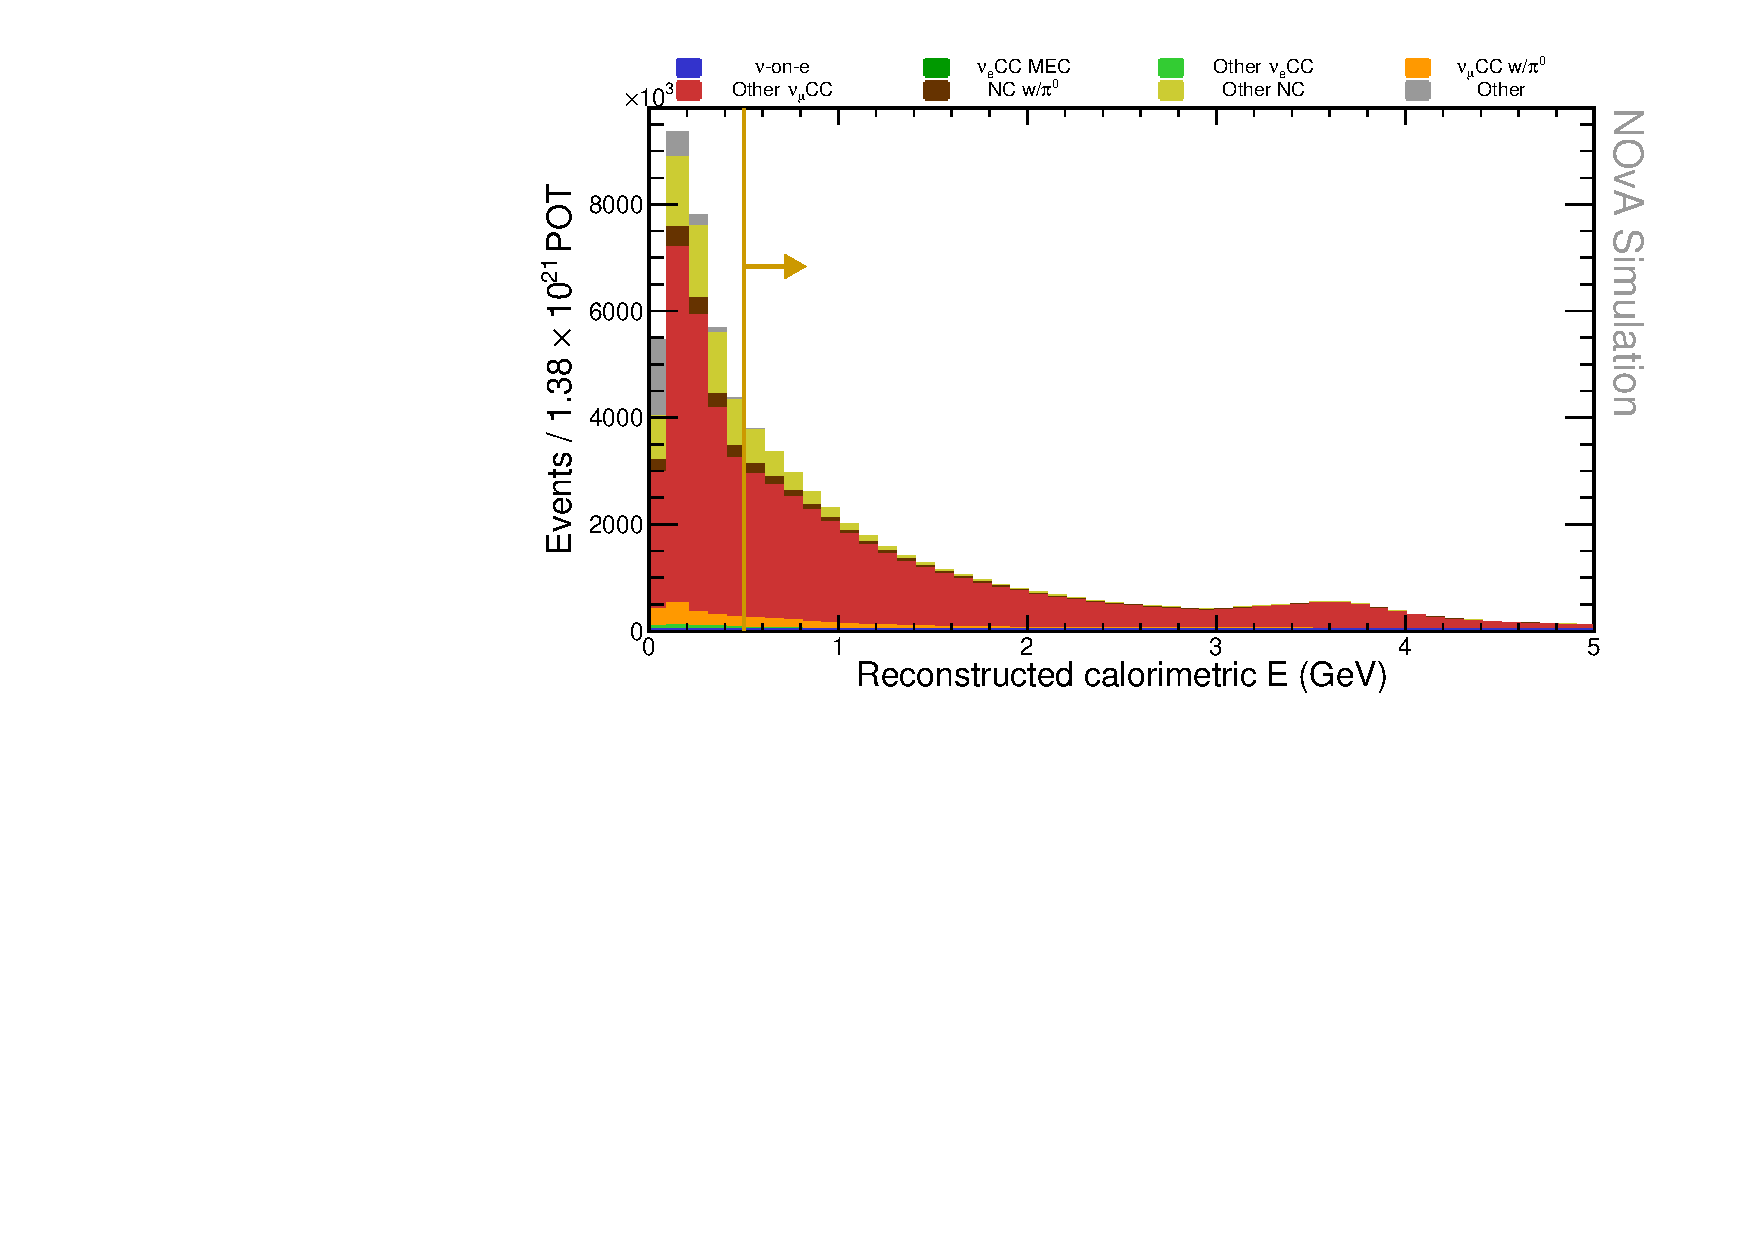
\includegraphics[width=.9\textwidth]{Plots/NuMMEventSelection/N1Cut_calELow_BkgDecomp.pdf}
\caption[Low calorimetric energy cut for reconstruction quality]{Top: Relative comparison of signal (red), \acrshort{nuone} background (blue), and other background (green) events in the reconstructed calorimetric energy distribution. All histograms are area-normalised. Bottom: Decomposition of background into various sub-samples, normalised to the data \acrshort{POT} exposure. Events in both plots are required to have a valid reconstructed vertex, at least one reconstructed prong and less than $6$ hits per plane. Yellow lines indicate the cut value for the reconstructed calorimetric energy, with arrows pointing towards the preserved events.}
\label{fig:NuMMCutsLowCalE}
\end{figure}

\begin{table}[!hb]
\centering
\caption[Event selection cutflow table for the reconstruction quality cuts]{Event selection cutflow table for the reconstruction quality cuts showing the number of events and the relative efficiency of each cut for each signal sample. The relative efficiency is calculated as number of events remaining after applying the corresponding cut divided by number of events for all the previous cuts. All the cuts are listed in sequence as they are applied.}
\begin{tabular}{|l|cc|cc|cc|}\hline
\multicolumn{1}{|c|}{} & \multicolumn{2}{c|}{\textbf{Signal}} & \multicolumn{2}{c|}{\textbf{$\nu$-on-e bkg}} & \multicolumn{2}{c|}{\textbf{Other bkg}} \\
\multicolumn{1}{|c|}{\multirow{-2}{*}{\textbf{Selection}}} & \textbf{$N_{evt}$} & \textbf{$\epsilon_{rel}\left(\%\right)$} & \textbf{$N_{evt}$} & \textbf{$\epsilon_{rel}\left(\%\right)$}  & \textbf{$N_{evt}$} & \textbf{$\epsilon_{rel}\left(\%\right)$}\\\hline
\textbf{No Cut} & 817.34 & 100 & 6.82$\times 10^3$ & 100 & 2.96$\times 10^8$ & 100\\
\textbf{Valid Vtx} & 553.86 & 67.76 & 6.17$\times 10^3$ & 90.55 & 2.34$\times 10^8$ & 79.10\\
\textbf{N$^o$ Prongs} & 472.90 & 85.38 & 5.08$\times 10^3$ & 82.25 & 8.66$\times 10^7$ & 37.00\\
\textbf{Hits / Plane} & 471.14 & 99.63 & 4.97$\times 10^3$ & 97.85 & 7.32$\times 10^7$ & 89.56\\
\textbf{Low $E_{Shower}$} & 156.37 & 33.19 & 3.53$\times 10^3$ & 71.09 & 4.06$\times 10^7$ & 55.12\\\hline
\end{tabular}
\label{tab:CutflowTableBasicRecoQC}
\end{table}

\subsection{Pre-selection}\label{sec:NuMMEventSelectionPresel}
Pre-selection aims to remove obvious background events without significantly affecting the signal. The criterion we chose for the selection of these cuts is determined by the reduction of the signal efficiency by approximately $\unit[0.25]{\%}$ with each cut. This results in the total pre-selection reduction of the signal efficiency by approximately $\unit[1]{\%}$.

The first two variables used for our pre-selection are the same as were used in the event selection for the $\nu_e$ appearance \gls{ND} constraint for the three flavour neutrino oscillation measurements \cite{NOvAResults2021.pdf}. As we are searching for single electron showers, we can reduce backgrounds with multiple final state particles by limiting the total activity in the detector. Specifically, we require that the total number of hits assigned to all the reconstructed prongs is $<280$. This is shown in Fig.~\ref{fig:NuMMCutsNHitsLoose}. In general, the main background in \gls{NOvA} consists of the $\nu_\mu$\gls{CC} interactions, which are characterised by long muon tracks. We therefore limit the length of the longest reconstructed prong to be $<\unit[640]{cm}$, as shown in Fig.~\ref{fig:NuMMCutsLongestProng}. 

\begin{figure}[hbtp]
\centering
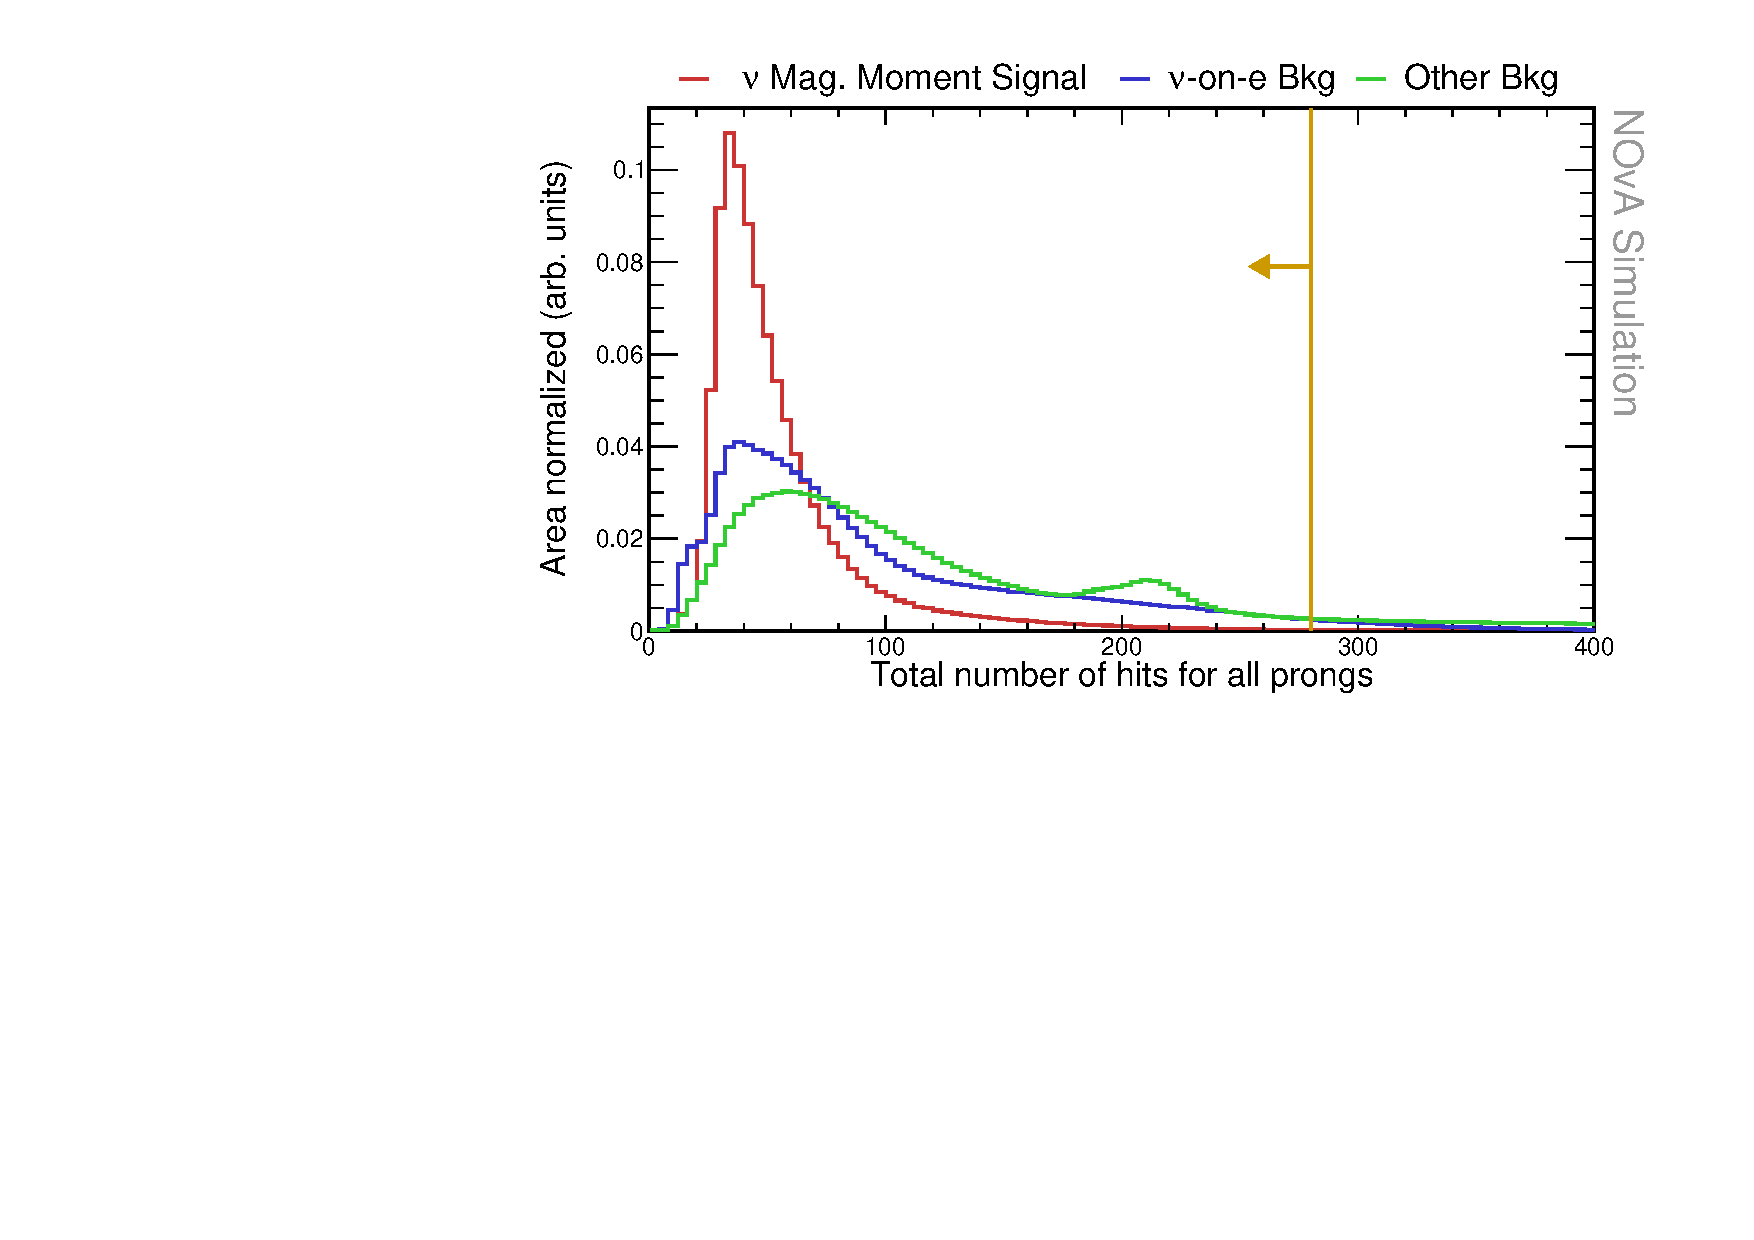
\includegraphics[width=.9\textwidth]{Plots/NuMMEventSelection/N1Cut_NHitsLoose.pdf}
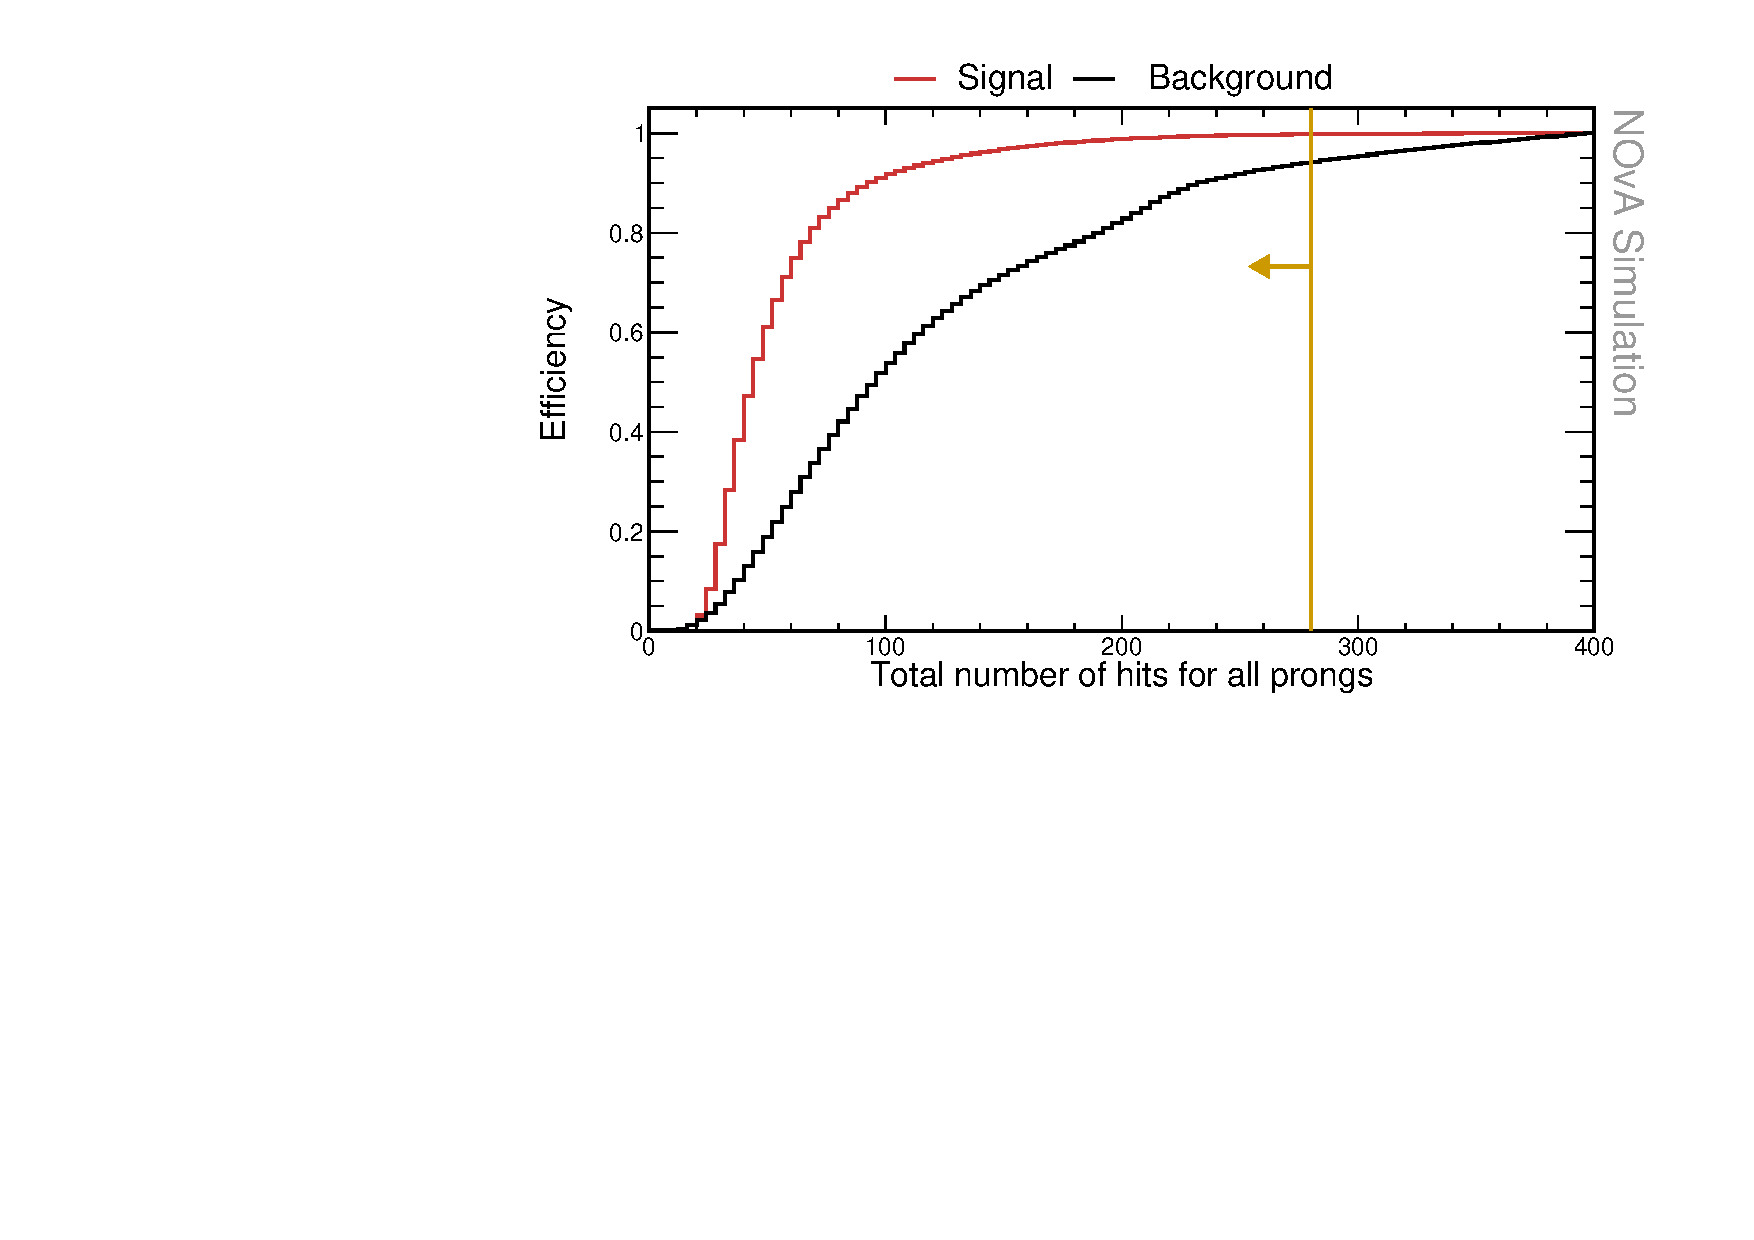
\includegraphics[width=.9\textwidth]{Plots/NuMMEventSelection/NuMM_N1Cut_NHitsLooseleft_Eff.pdf}
\caption[Number of hits cut for pre-selection]{Top: Relative comparison of signal (red), \acrshort{nuone} background (blue), and other background (green) events in the distribution of total number of hits from all reconstructed prongs in the slice. All histograms are area-normalised. Bottom: Cumulative signal (red) and background (black) efficiency calculated as number of signal/background events left of the bin divided by the total number of signal/background events. Yellow lines indicate the cut value for the maximum number of hits, with arrows pointing towards the preserved events. The reconstruction quality cuts were applied before making these plots.}
\label{fig:NuMMCutsNHitsLoose}
\end{figure}

\begin{figure}[hbtp]
\centering
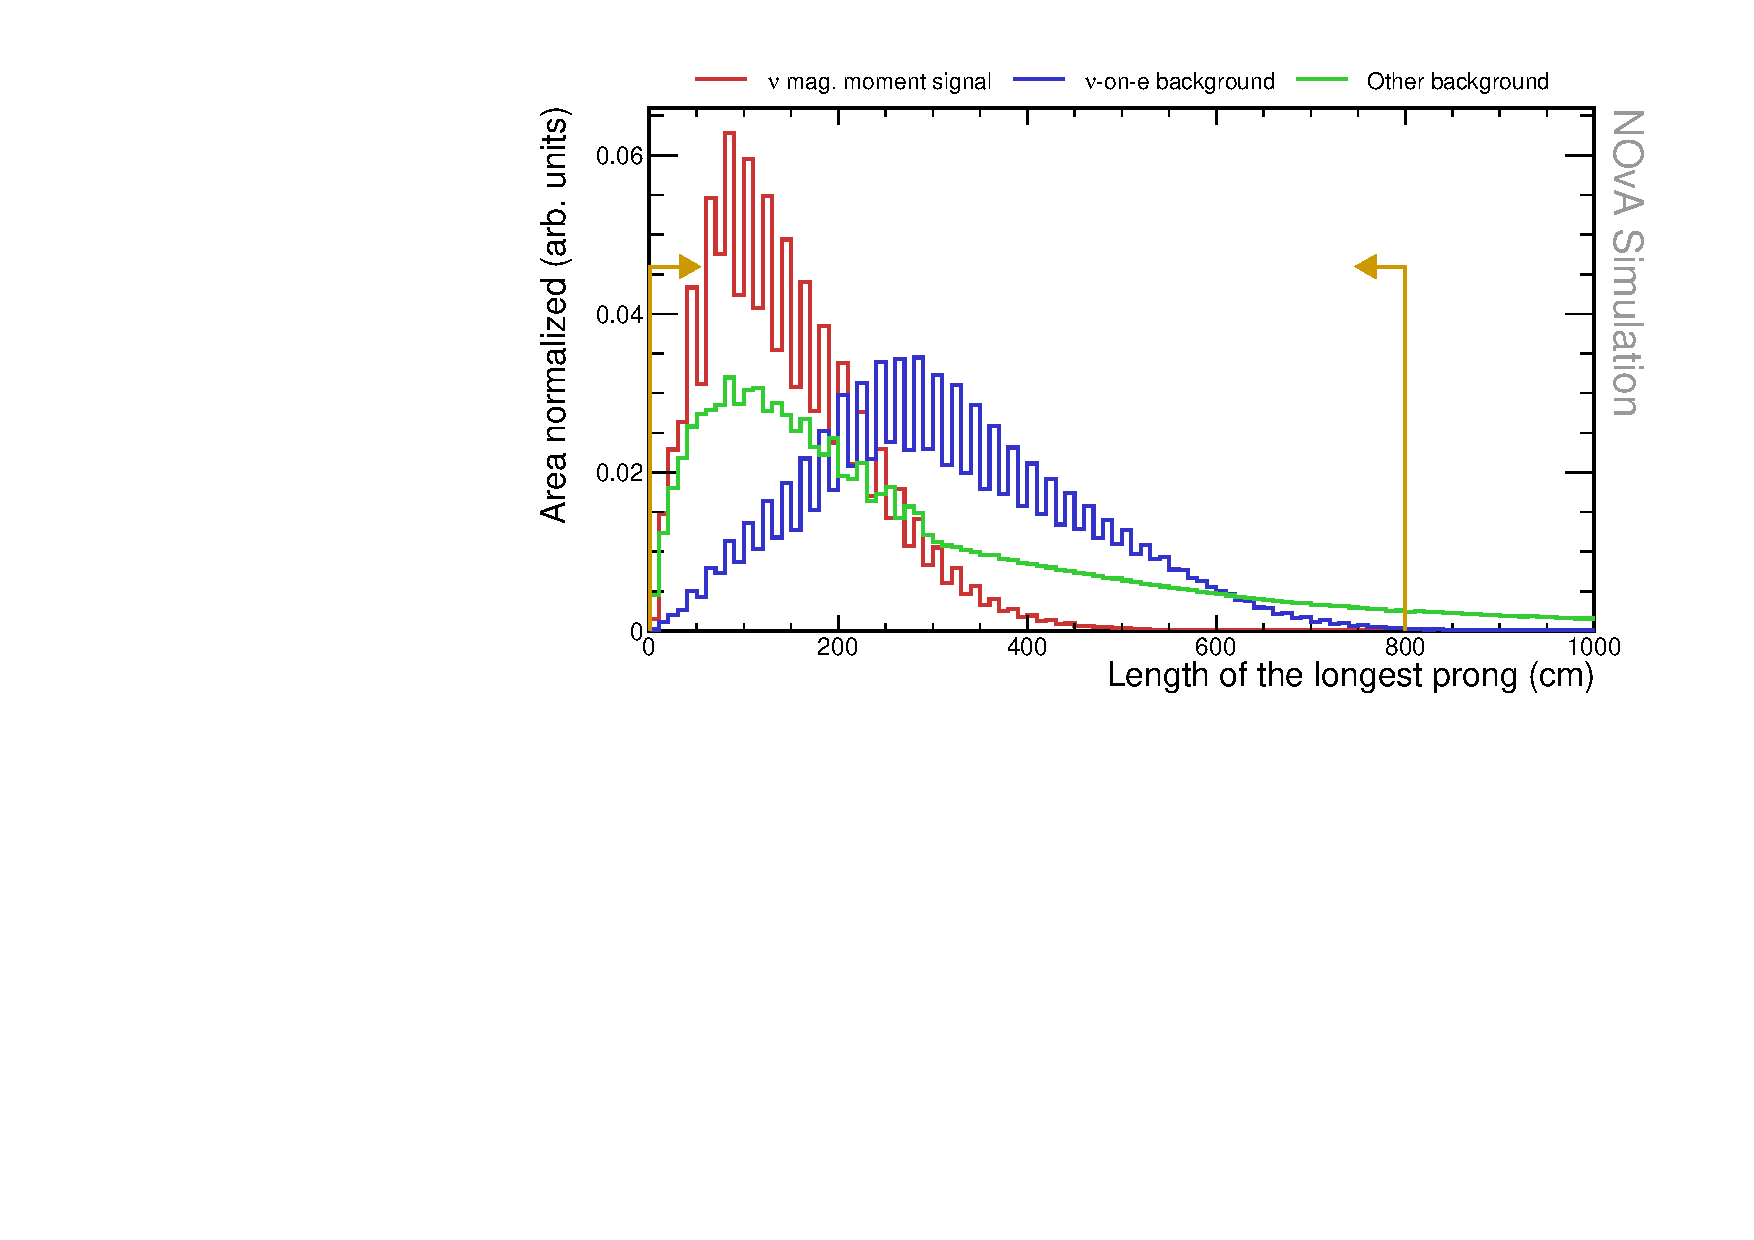
\includegraphics[width=.9\textwidth]{Plots/NuMMEventSelection/N1Cut_longestProng.pdf}
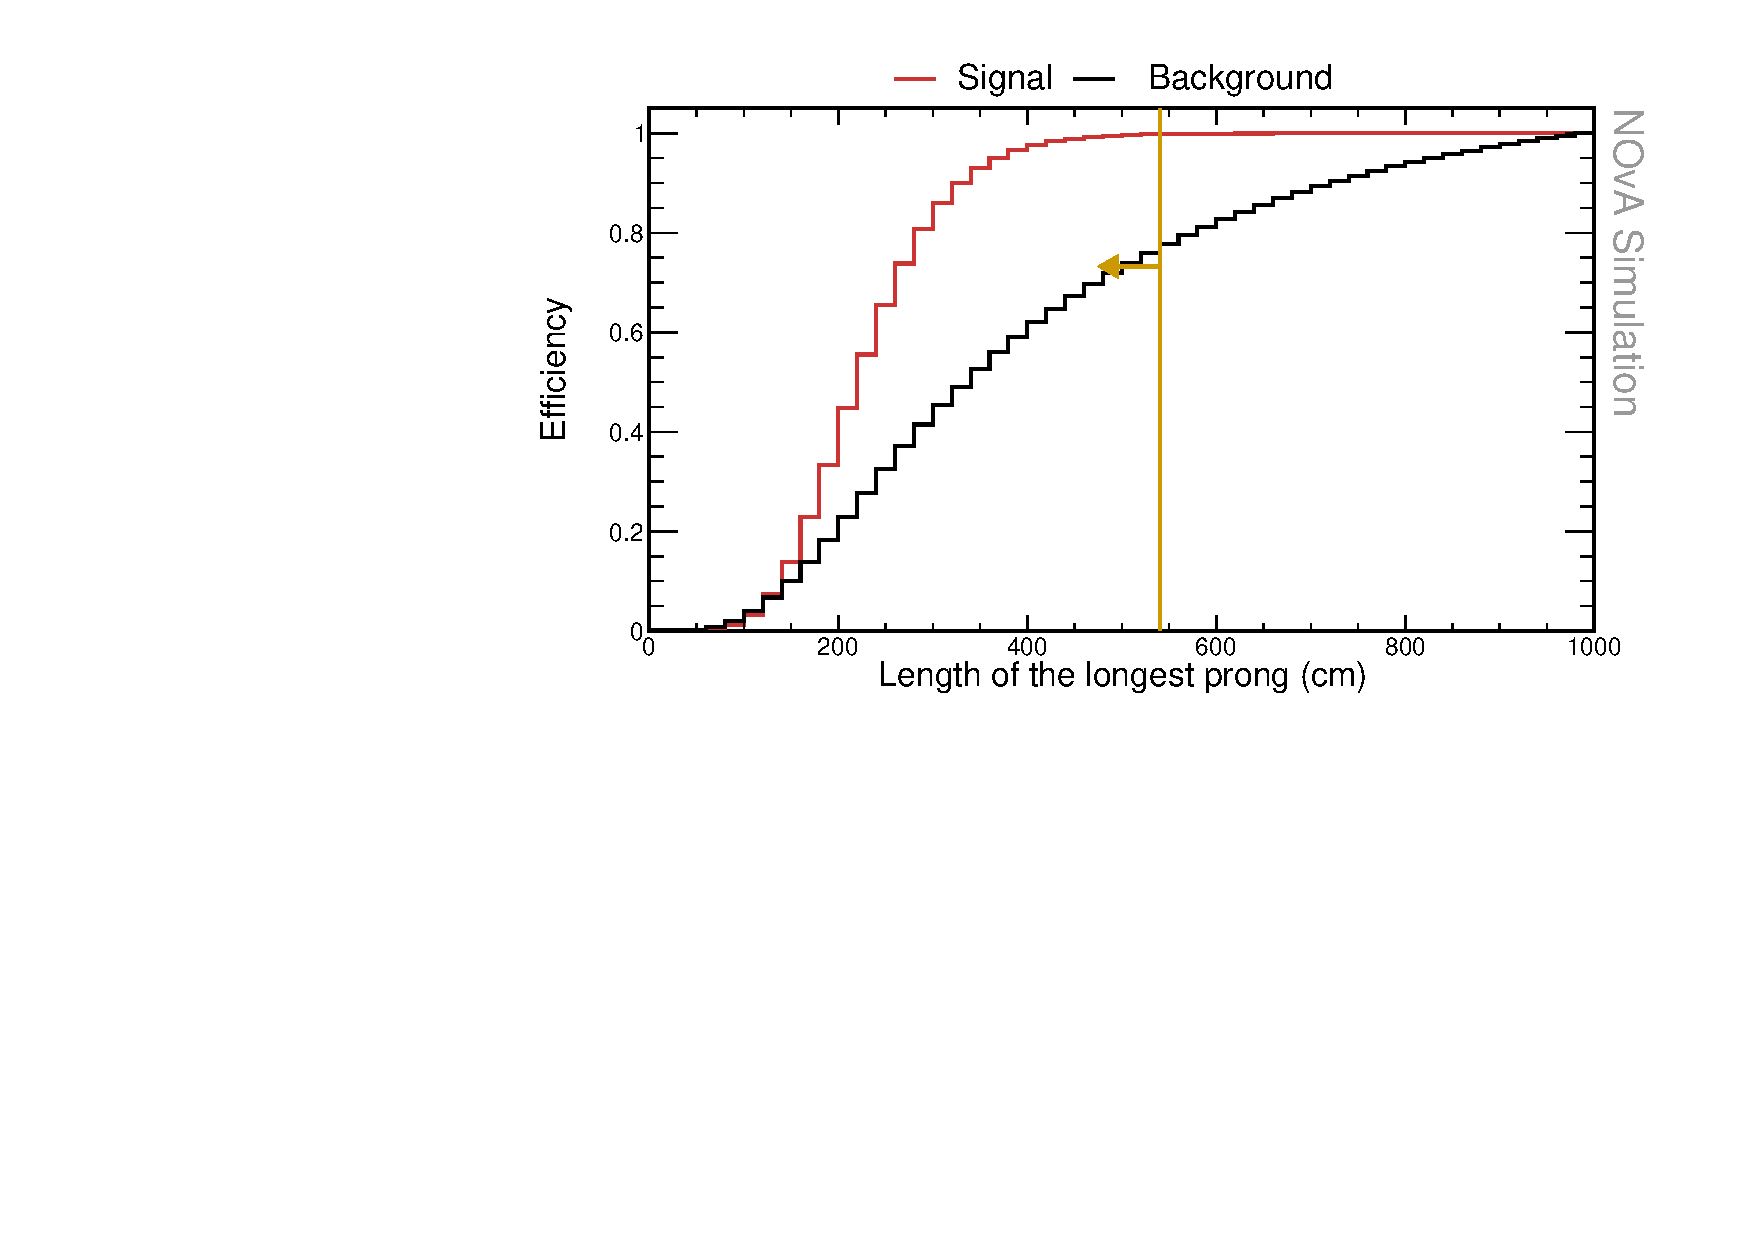
\includegraphics[width=.9\textwidth]{Plots/NuMMEventSelection/NuMM_N1Cut_longestProngleft_Eff.pdf}
\caption[Length of the longest prong cut for pre-selection]{Top: Relative comparison of signal (red), \acrshort{nuone} background (blue), and other background (green) events in the distribution of the length of the longest reconstructed prong in slice. All histograms are area-normalised. Bottom: Cumulative signal (red) and background (black) efficiency calculated as number of signal/background events left of the bin divided by the total number of signal/background events. Yellow lines indicate the cut value for the maximum length of the longest prong, with arrows pointing towards the preserved events. The reconstruction quality cuts and the number of hits cut were applied before making these plots.}
\label{fig:NuMMCutsLongestProng}
\end{figure}

Additionally, as discussed in Sec.~\ref{sec:MeasuringNuMM}, simple $2\rightarrow2$ kinematics dictate that the true electron recoil energy and angle for the \gls{nuone} interaction are limited by $E\theta^2<2m_e$. This can be used to distinguish \gls{nuone} elastic scattering from $\nu_e$\gls{CC} interactions, which also have an electron in the final state. However, due to unavoidable reconstruction deficiencies, the reconstructed $E\theta^2$ does not have such a strict cut-off value, and we are placing the pre-selection cut at $E\theta^2<0.064$, as can be seen in Fig.~\ref{fig:NuMMCutsETh2Loose}. Furthermore, some of the signal events can be reconstructed with the opposite direction with respect to the beam, which would result in $\theta\approx\unit[\pi]{rad}$. However, this reconstruction failure likely does not impact other reconstructed qualities and these events should be preserved for the final sample. For that reason, we are calculating the angle between the outgoing electron and the neutrino beam direction as $\arccos\left(\textsf{abs}\left(\cos\theta\right)\right)$, which gives the same value whether the shower is reconstructed forward or backwards.

\begin{figure}[hbtp]
\centering
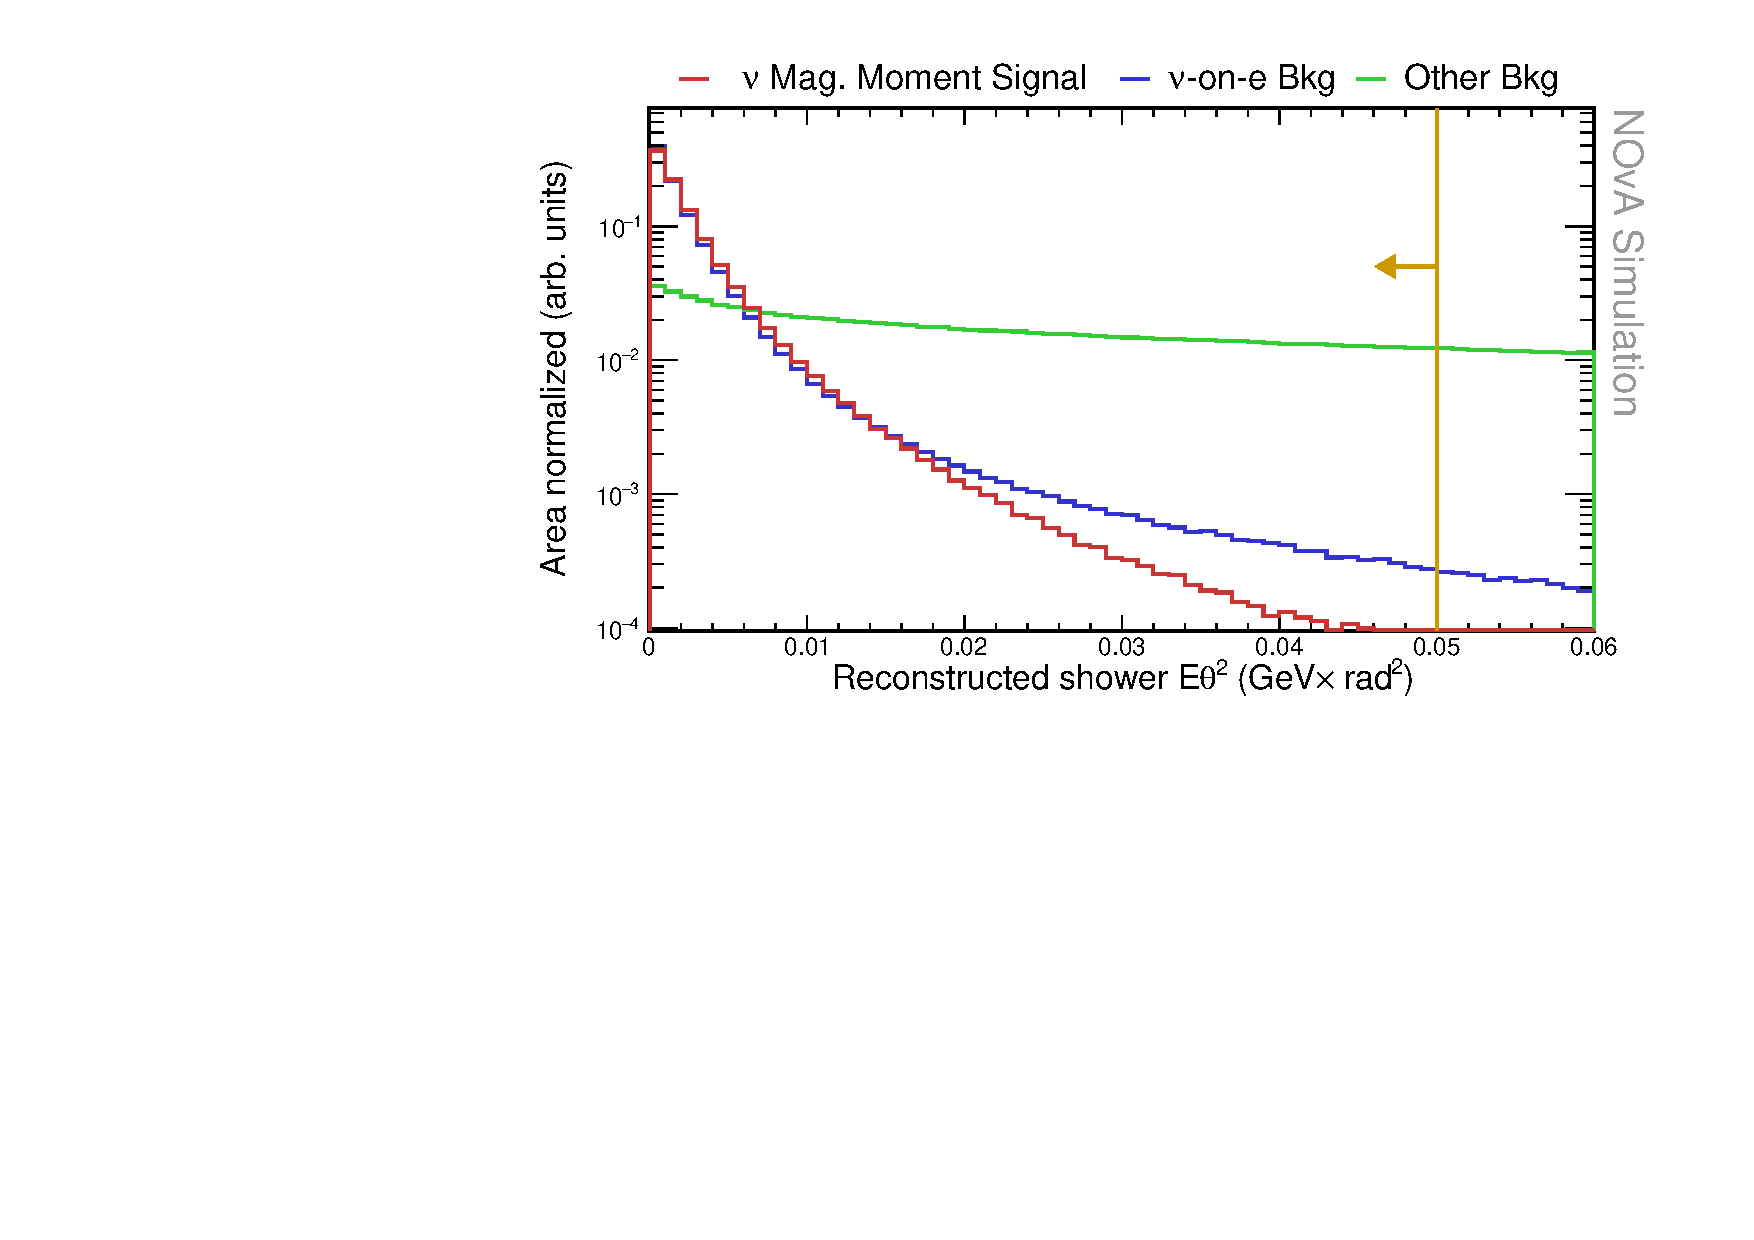
\includegraphics[width=.9\textwidth]{Plots/NuMMEventSelection/LogY_N1Cut_eth2Loose.pdf}
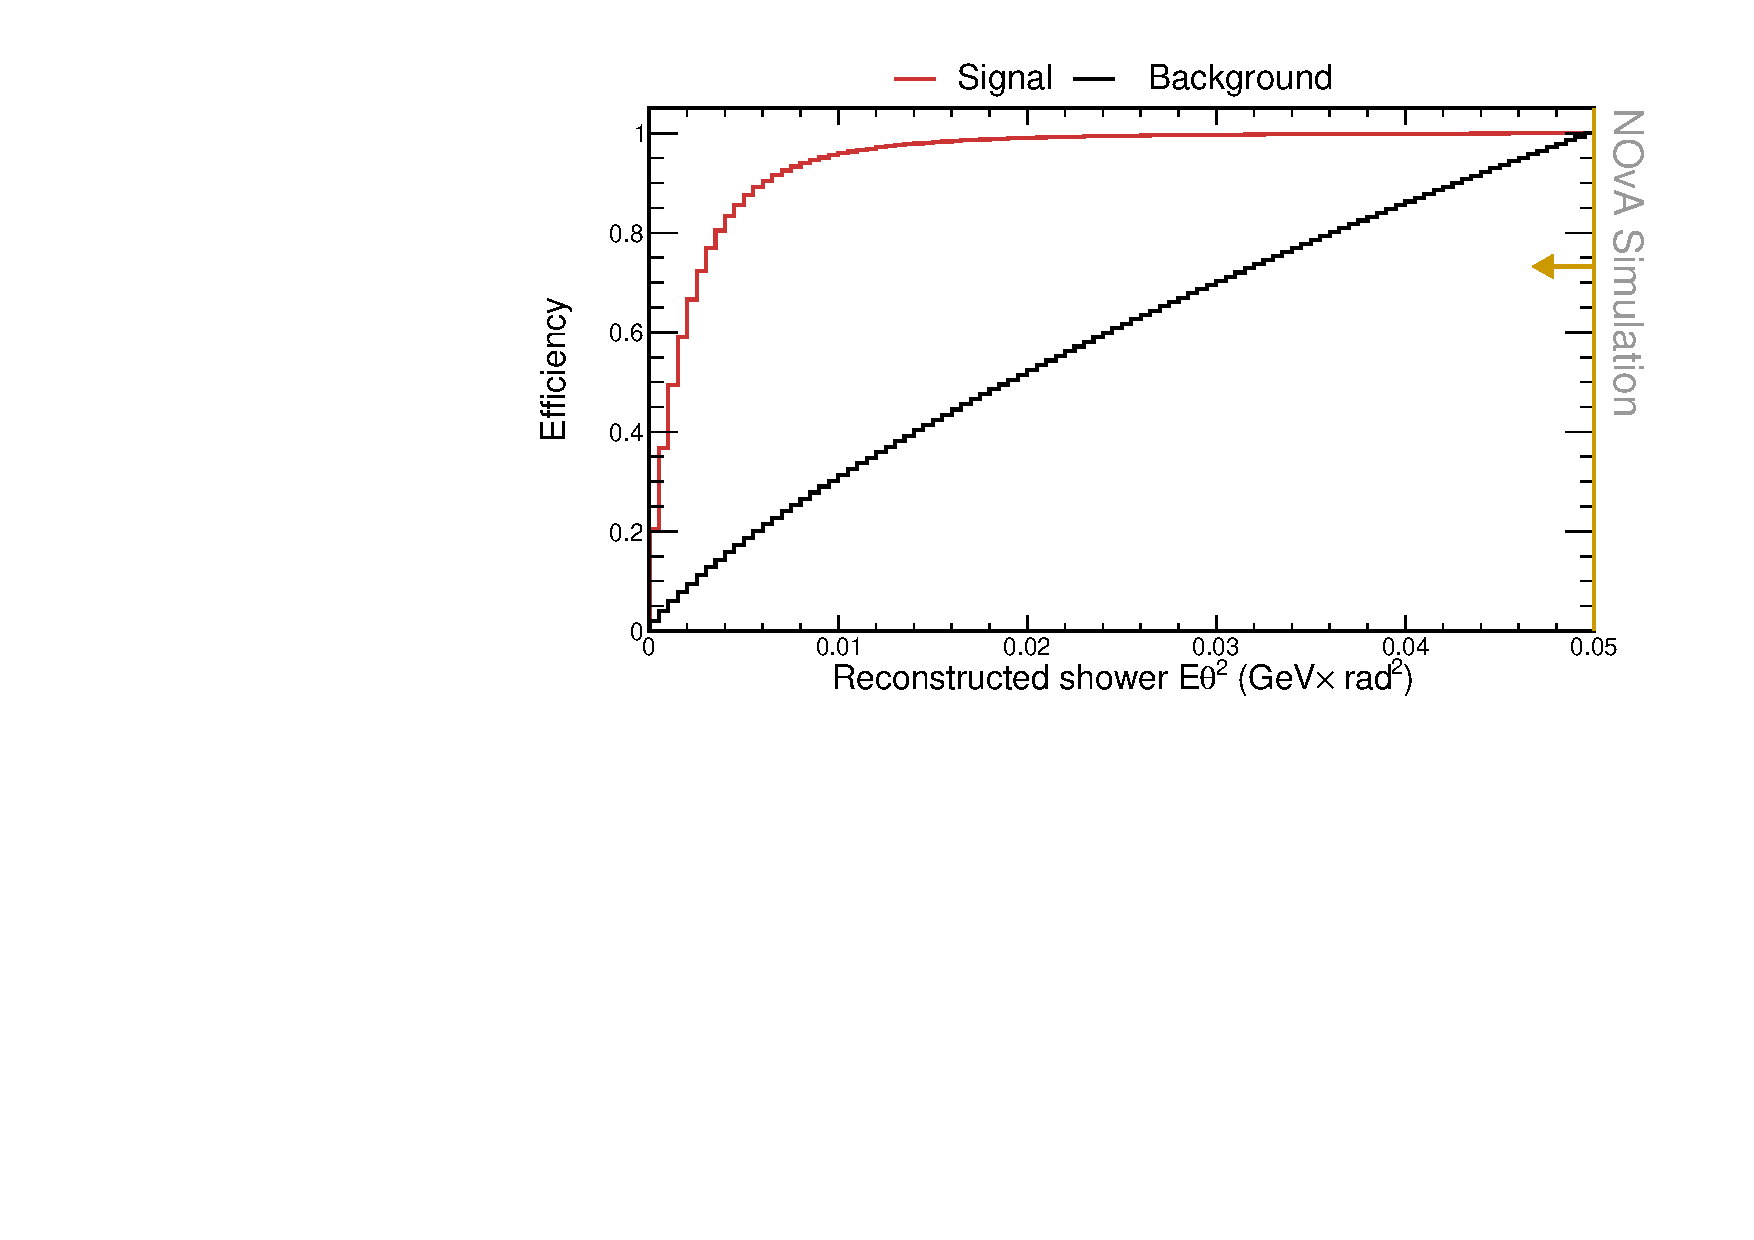
\includegraphics[width=.9\textwidth]{Plots/NuMMEventSelection/NuMM_N1Cut_eth2Looseleft_Eff.pdf}
\caption[$E\theta^2$ cut for pre-selection]{Top: Relative comparison of signal (red), \acrshort{nuone} background (blue), and other background (green) events in the distribution of the reconstructed energy of the leading shower multiplied by its angle from the incoming neutrino beam direction squared. All histograms are area-normalised with logarithmic y axis. Bottom: Cumulative signal (red) and background (black) efficiency calculated as number of signal/background events left of the bin divided by the total number of signal/background events. Yellow lines indicate the cut value for the depicted variable, with arrows pointing towards the preserved events. The reconstruction quality cuts, the number of hits cut, and the length of the longest prong cuts were applied before making both of these plots.}
\label{fig:NuMMCutsETh2Loose}
\end{figure}

The effect of the pre-selection cuts on the signal and background samples are summarised in Tab.~\ref{tab:CutflowTableBasicSelection}, where the first row lists the number of events after applying all the reconstruction quality cuts from Sec.~\ref{sec:NuMMEventSelRecoQC}. All three of the variables used for the pre-selection are employed again in the \gls{MVA}, as described in Sec.~\ref{sec:NuMMEventSelTMVA}.

%\todo{Add the DeCAF cuts description here - might describe them already when introducing the decaf samples, not sure yet}

\begin{table}[!hb]
\centering
\caption[Event selection cutflow table for the pre-selection]{Pre-selection cutflow table showing the number of events and the relative efficiency of each cut for each signal sample. The relative efficiency is calculated as number of events remaining after applying the corresponding cut divided by number of events for all the previous cuts. All the cuts are listed in sequence as they are applied. The top row corresponds to the sample after applying the reconstruction quality cuts.}
\begin{tabular}{|l|cc|cc|cc|}\hline
\multicolumn{1}{|c|}{} & \multicolumn{2}{c|}{\textbf{Signal}} & \multicolumn{2}{c|}{\textbf{$\nu$-on-e bkg}} & \multicolumn{2}{c|}{\textbf{Other bkg}} \\
\multicolumn{1}{|c|}{\multirow{-2}{*}{\textbf{Selection}}} & \textbf{$N_{evt}$} & \textbf{$\epsilon_{rel}\left(\%\right)$} & \textbf{$N_{evt}$} & \textbf{$\epsilon_{rel}\left(\%\right)$}  & \textbf{$N_{evt}$} & \textbf{$\epsilon_{rel}\left(\%\right)$}\\\hline
\textbf{Reco Quality} & 156.37 & 100 & 3.53$\times 10^3$ & 100 & 4.28$\times 10^7$ & 100\\
\textbf{N$^o$ Hits Loose} & 156.05 & 99.79 & 3.41$\times 10^3$ & 96.46 & 3.61$\times 10^7$ & 84.35\\
\textbf{Prong Length} & 155.7 & 99.78 & 3.37$\times 10^3$ & 98.85 & 2.61$\times 10^7$ & 72.36\\
\textbf{$E\theta^2$ Loose} & 155.14 & 99.64 & 3.33$\times 10^3$ & 98.83 & 8.83$\times 10^6$ & 33.82\\\hline
\end{tabular}
\label{tab:CutflowTableBasicSelection}
\end{table}

\subsection{Fiducial and containment cuts}\label{sec:NuMMEventSelFidCont}
To ensure all the deposited energy of the recoil electron is contained within the detector and to remove events originating outside of the detector (such as rock muons for the \gls{ND}), we constrain the position of the reconstructed vertex and all the prongs in the slice. The decision on where to place the exact cut values is made based on the maximum \gls{FOM} value.

The reconstructed vertex is required to be within the fiducial volume, which represents a well-understood volume of the detector. To select the fiducial volume, we investigate distributions of the reconstructed vertex in the x, y and z direction, shown in Fig.~\ref{fig:NuMMFiducialCutX}, \ref{fig:NuMMFiducialCutY} and \ref{fig:NuMMFiducialCutZ} respectively. Basic reconstruction quality and pre-selection cuts are applied to make these distributions. Additionally, for the x and y position distributions, we require that the vertex is not placed inside of the Muon Catcher by requiring $\textsf{Vtx}_Z<\unit[1270]{cm}$, as it can significantly affect these distributions. The slanted distributions in x and y are caused by the off-axis nature of the \gls{NuMI} beam and the periodic peaks are due to a combination of the detector structure and the choice of binning.

The reconstructed vertex is required to be contained within the following volume:
\begin{align}
\unit[-175]{cm}<&\textsf{Vtx}_X<\unit[175]{cm},\\
\unit[-175]{cm}<&\textsf{Vtx}_Y<\unit[175]{cm},\\
\unit[95]{cm}<&\textsf{Vtx}_Z<\unit[1170]{cm}.
\end{align}

\begin{figure}[hbtp]
\centering
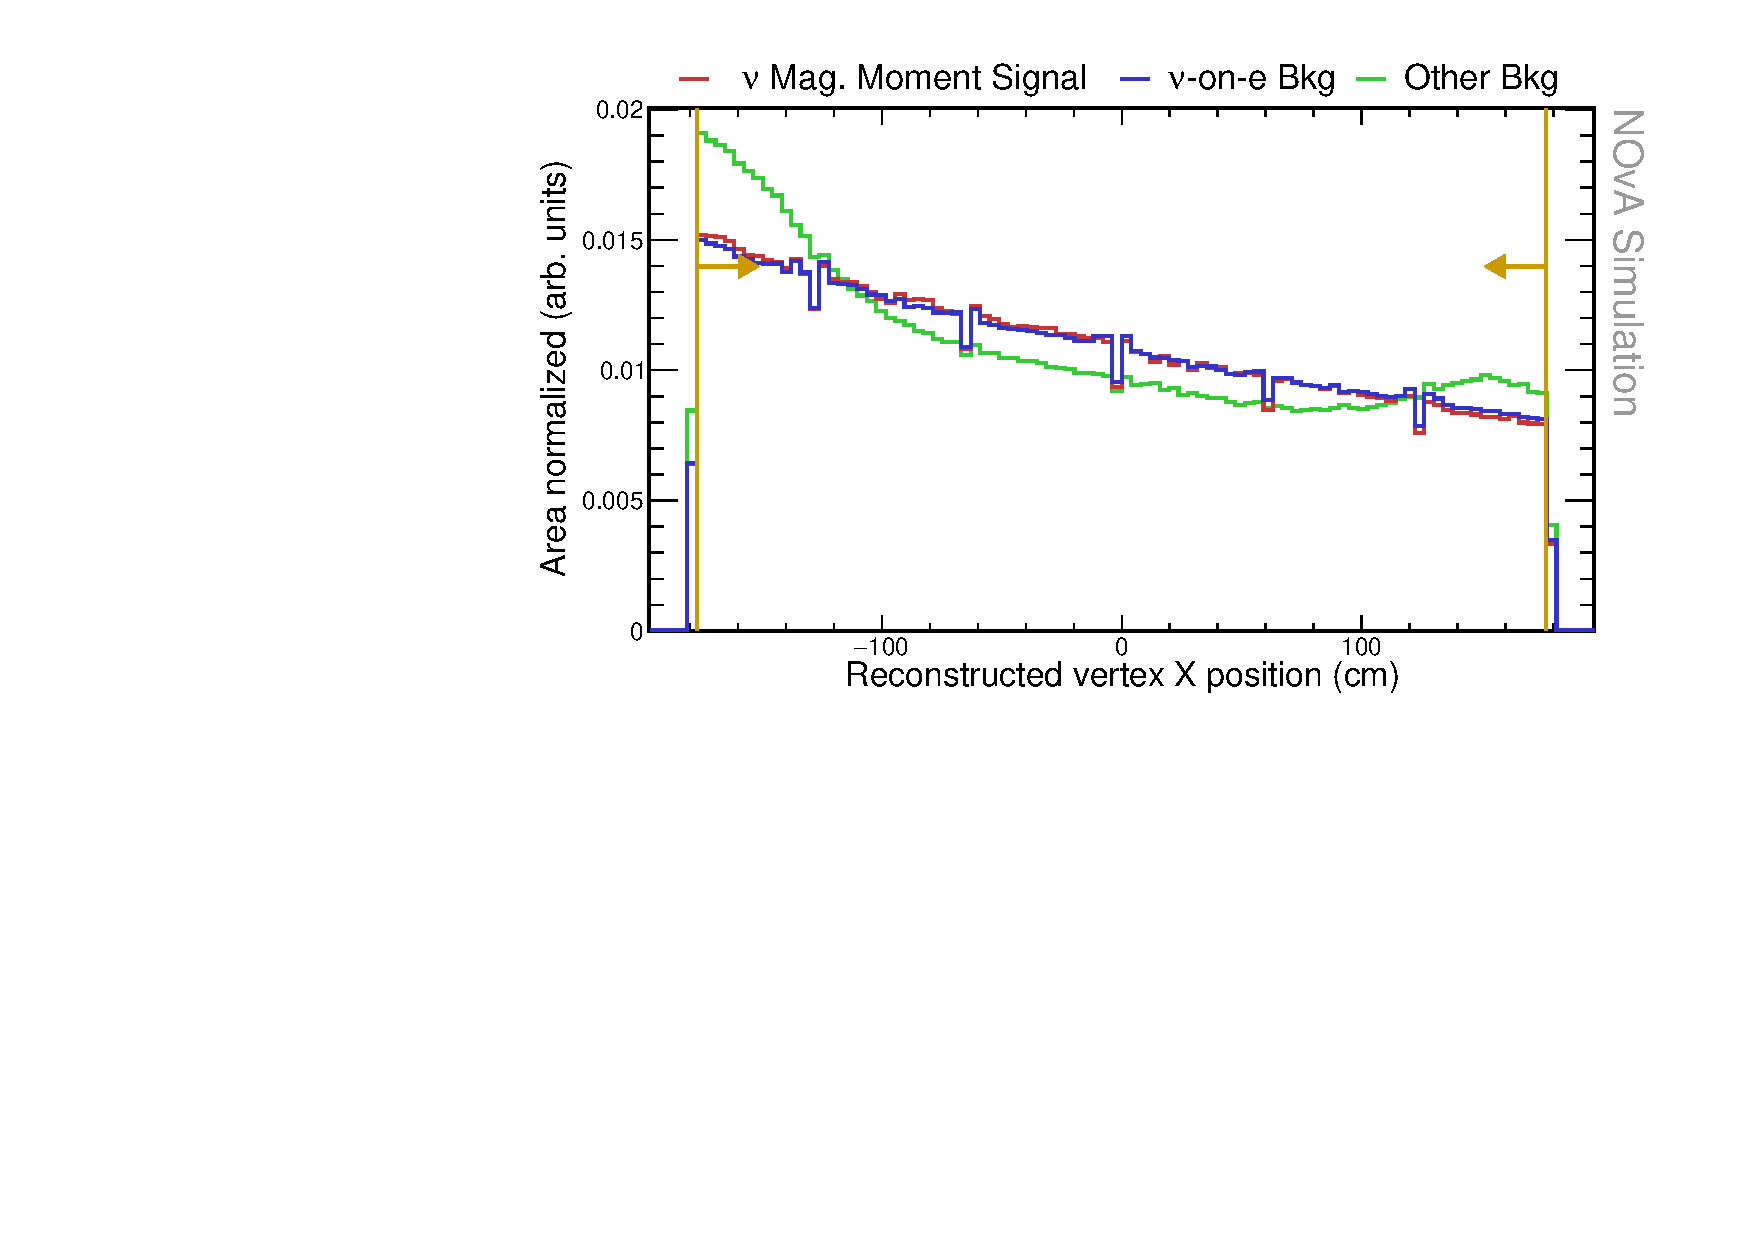
\includegraphics[width=.9\textwidth]{Plots/NuMMEventSelection/N1Cut_vtxXActive.pdf}
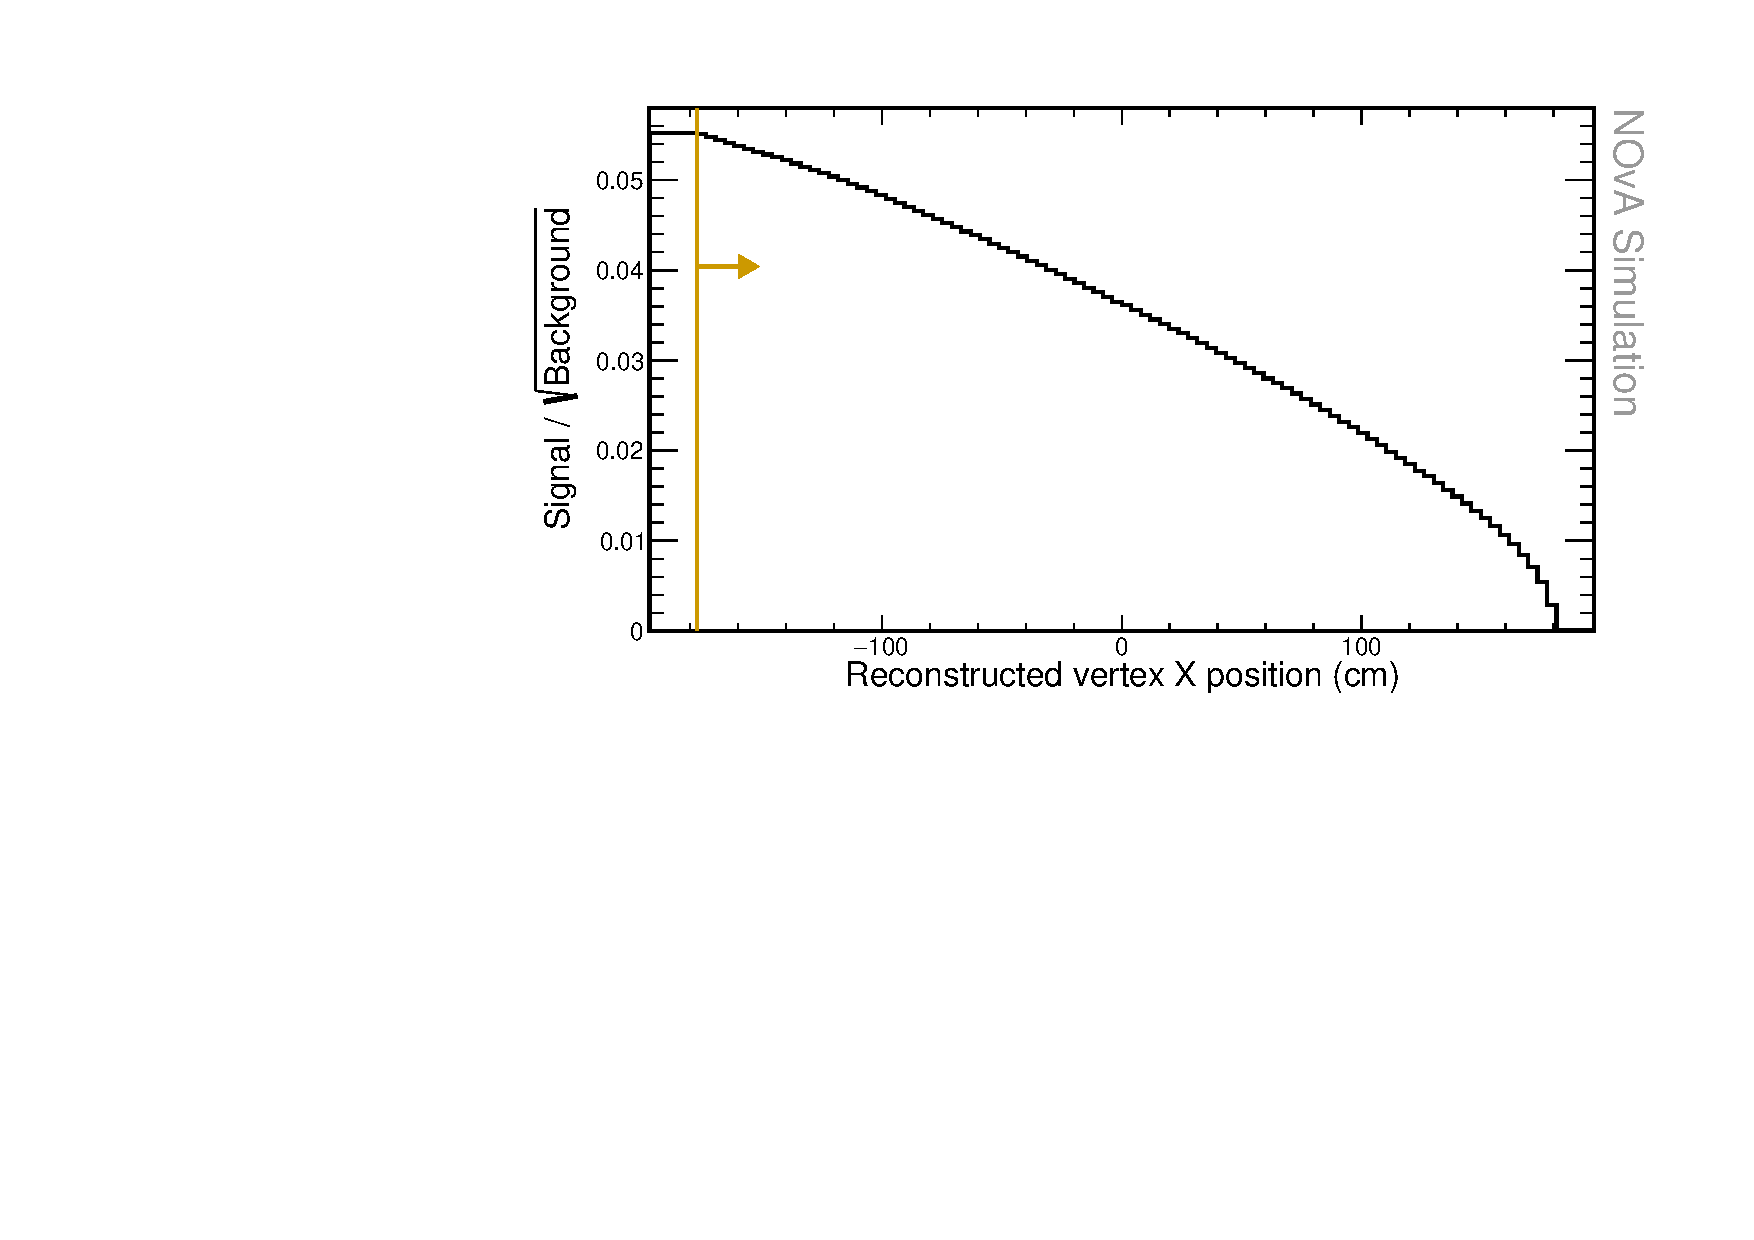
\includegraphics[width=.9\textwidth]{Plots/NuMMEventSelection/NuMM_N1Cut_vtxXActiveright_FOMStats.pdf}
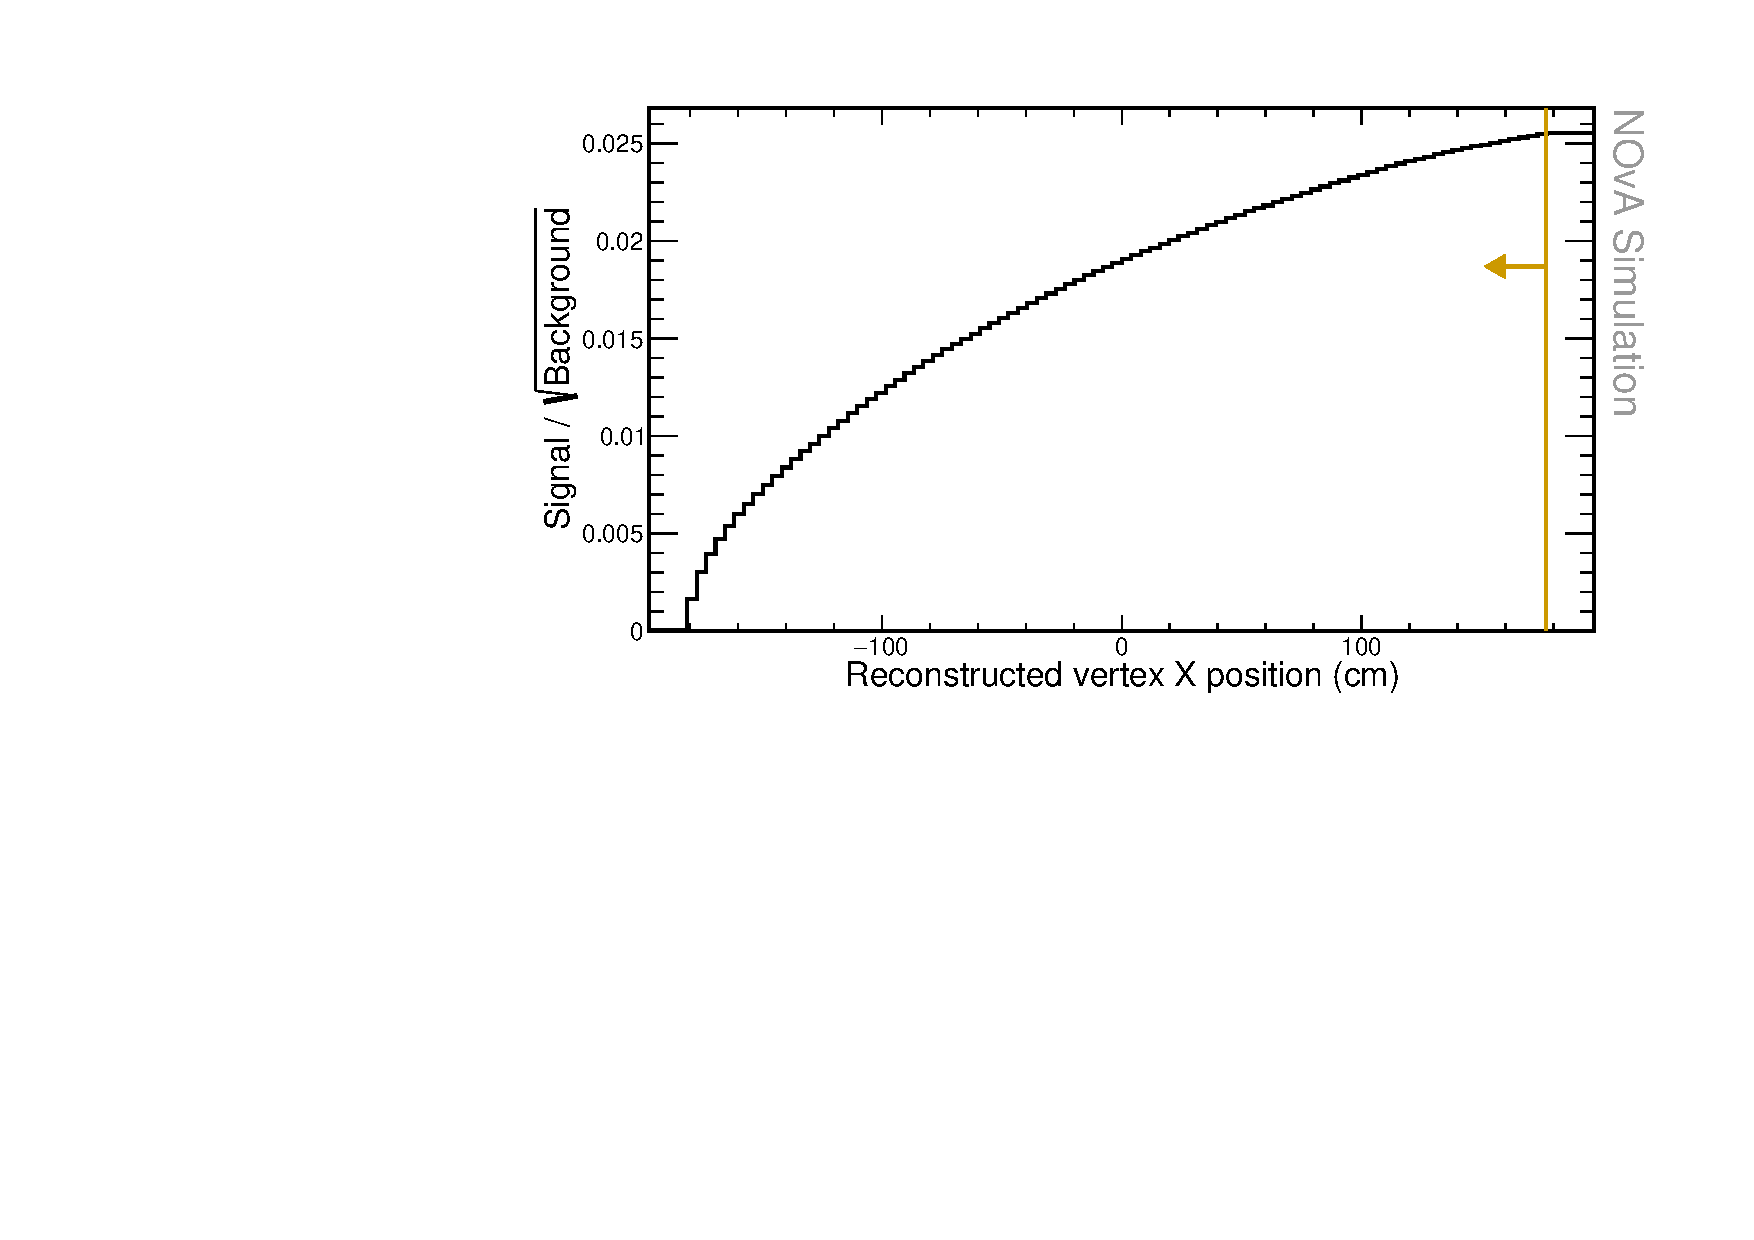
\includegraphics[width=.9\textwidth]{Plots/NuMMEventSelection/NuMM_N1Cut_vtxXActiveleft_FOMStats.pdf}
\caption[Vertex x containment cut]{Top: Relative comparison of signal (red), \acrshort{nuone} background (blue), and other background (green) events in the distribution of the x position of the reconstructed vertex. All histograms are area-normalized. Middle and bottom: Cumulative \acrshort{FOM} calculated as the number of signal events, divided by the number of background events from that bin until the end of the plot to the right (middle) or left (bottom). The reconstruction quality and pre-selection cuts were applied prior to making these plots. Additionally, vertex is required to be within the active region of the detector ($Vtx_Z<\unit[1270]{cm}$). Yellow lines show the cut values that create the fiducial volume, with arrows pointing towards the preserved events.}
\label{fig:NuMMFiducialCutX}
\end{figure}

\begin{figure}[hbtp]
\centering
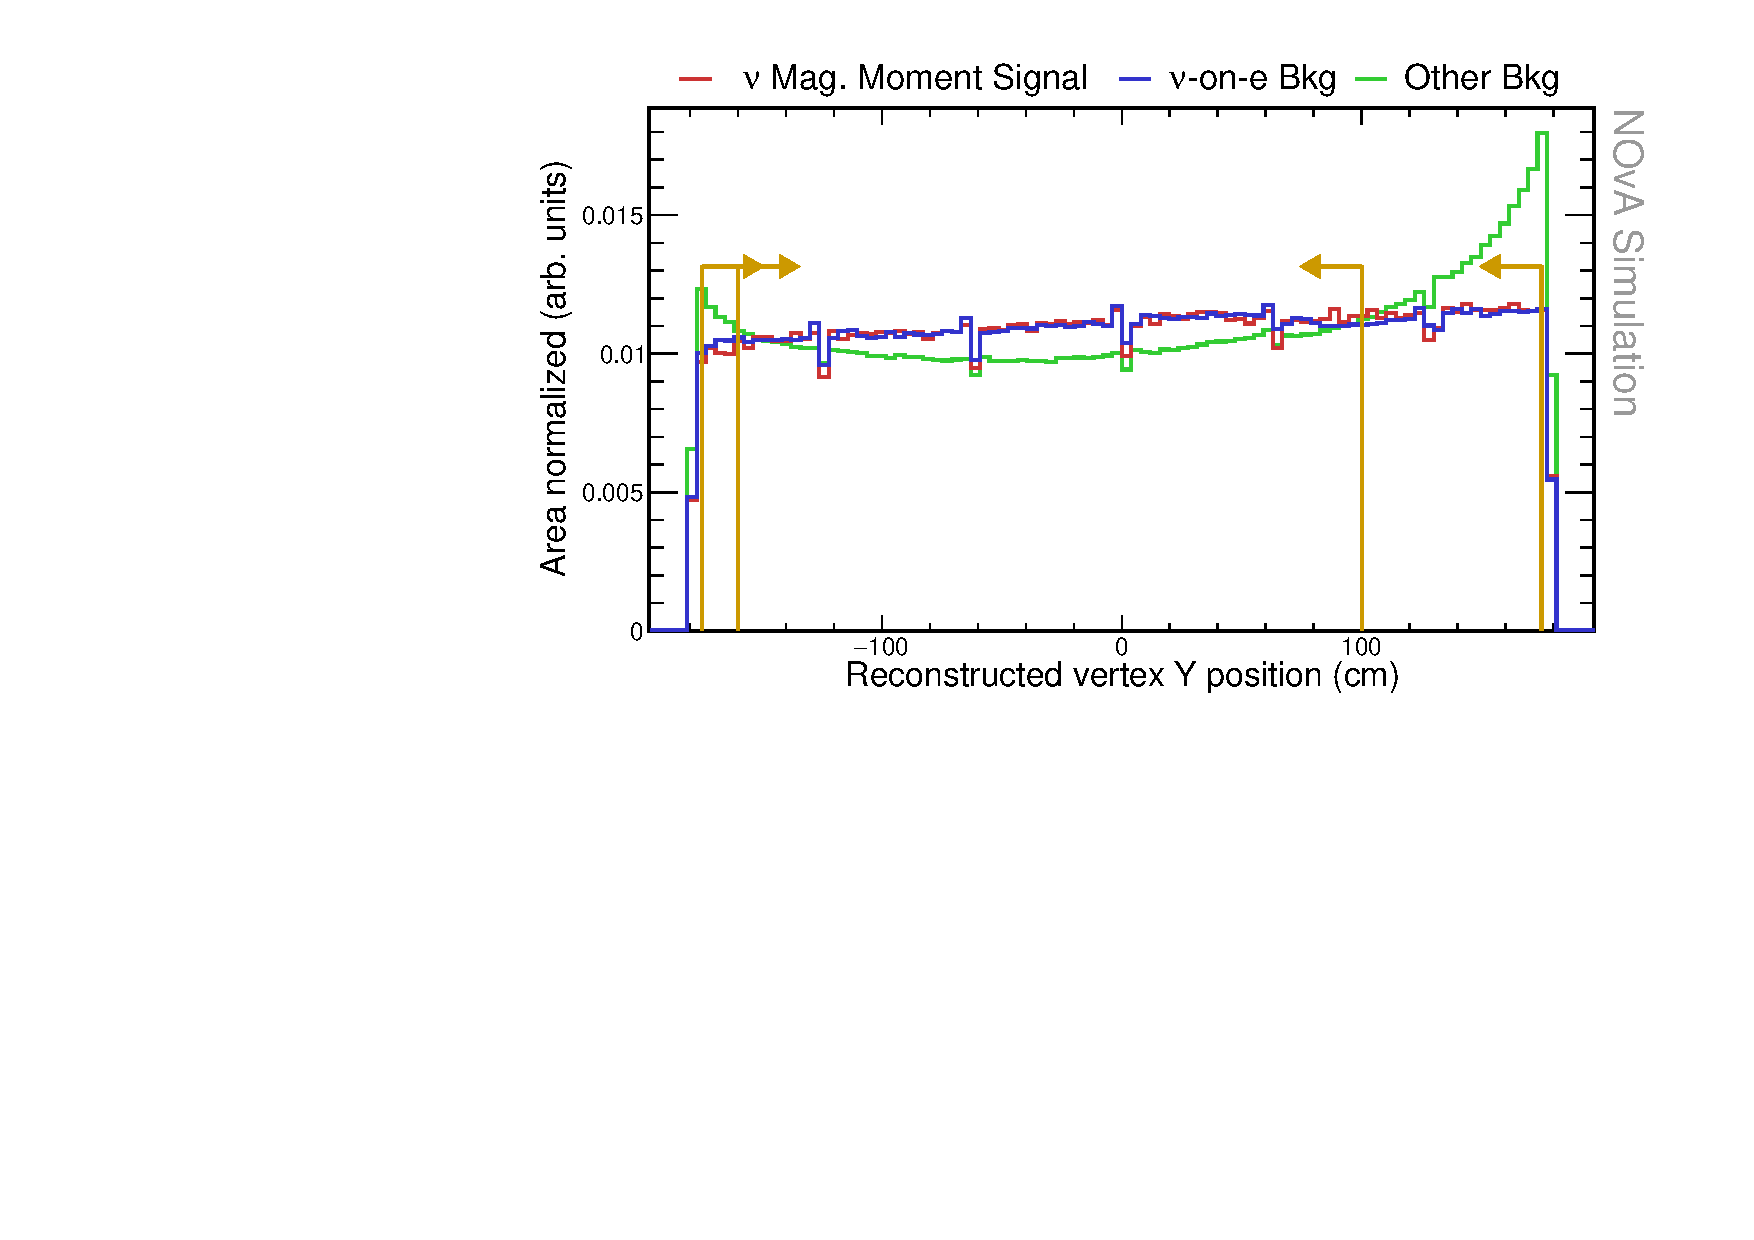
\includegraphics[width=.9\textwidth]{Plots/NuMMEventSelection/N1Cut_vtxYActive.pdf}
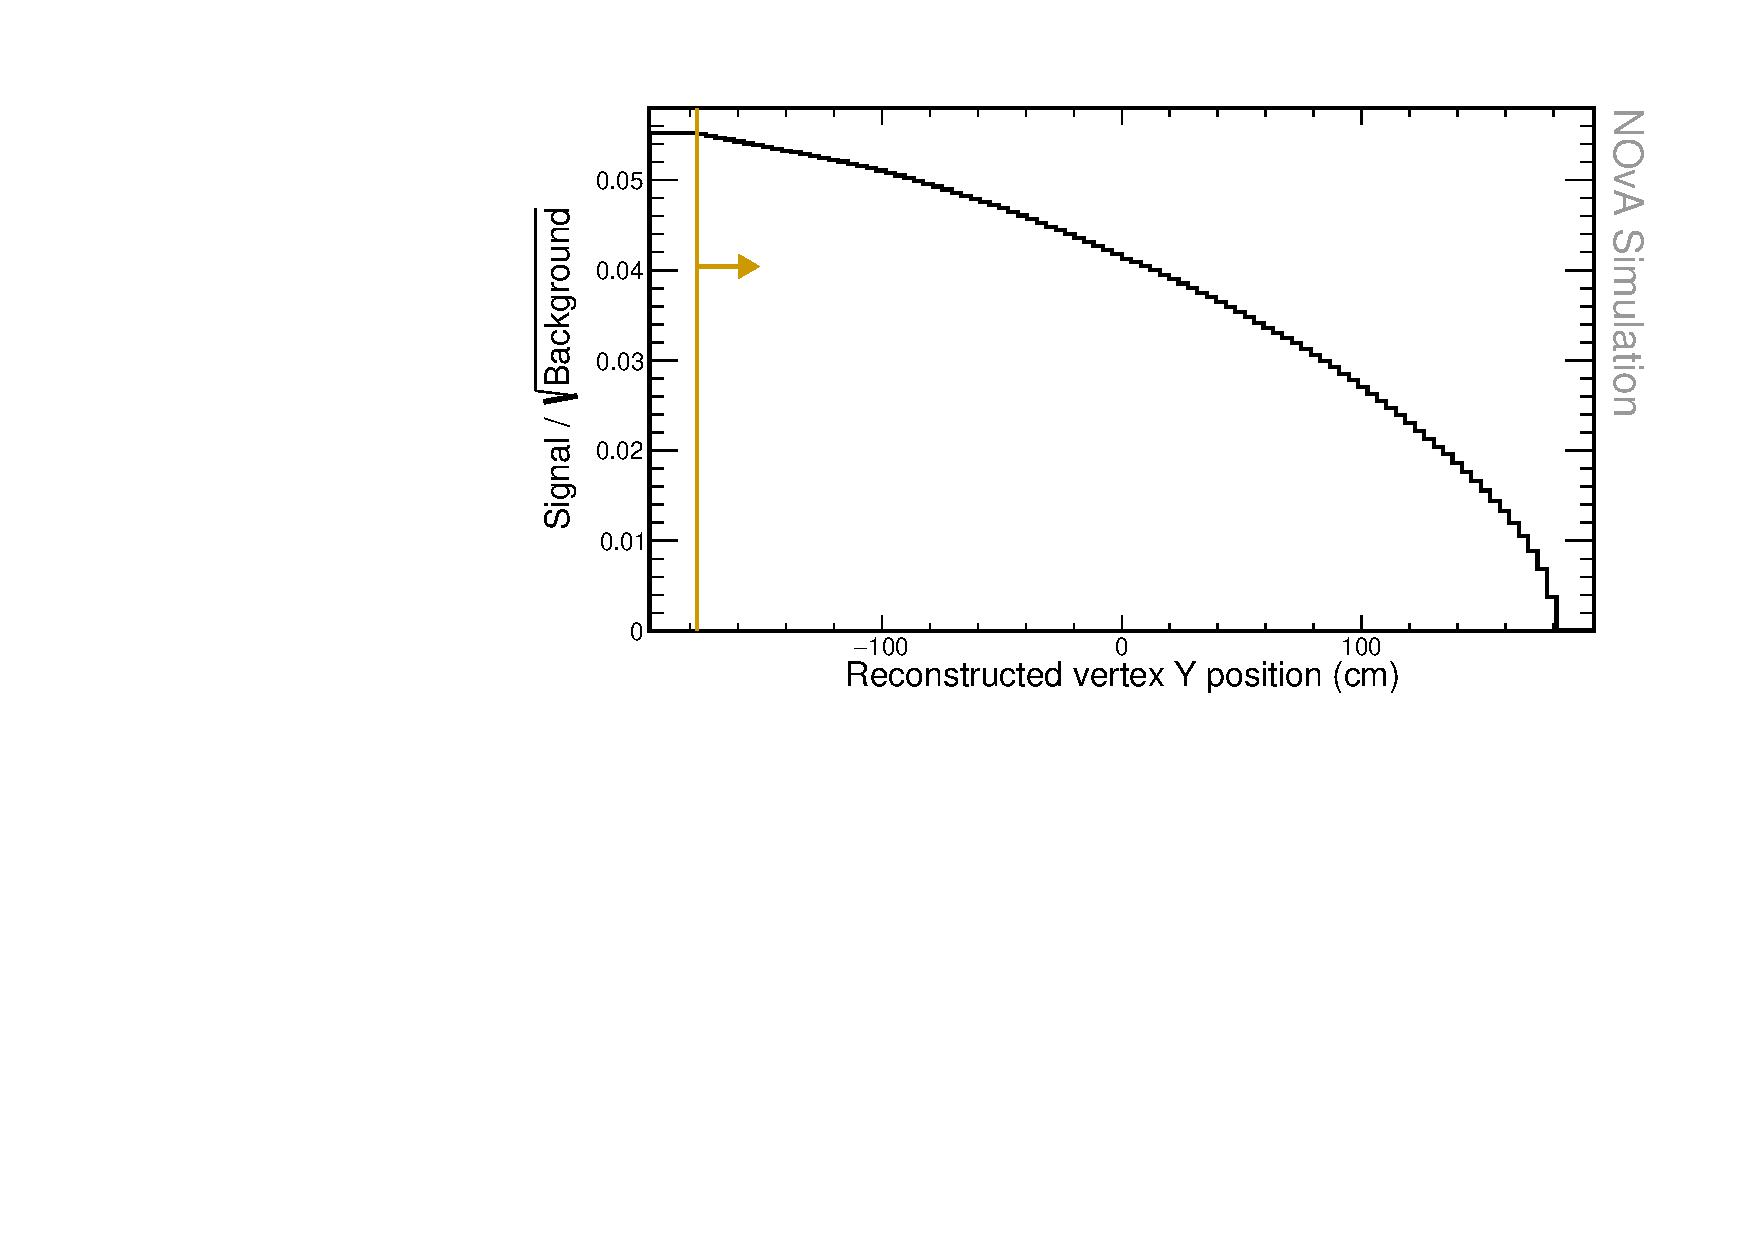
\includegraphics[width=.9\textwidth]{Plots/NuMMEventSelection/NuMM_N1Cut_vtxYActiveright_FOMStats.pdf}
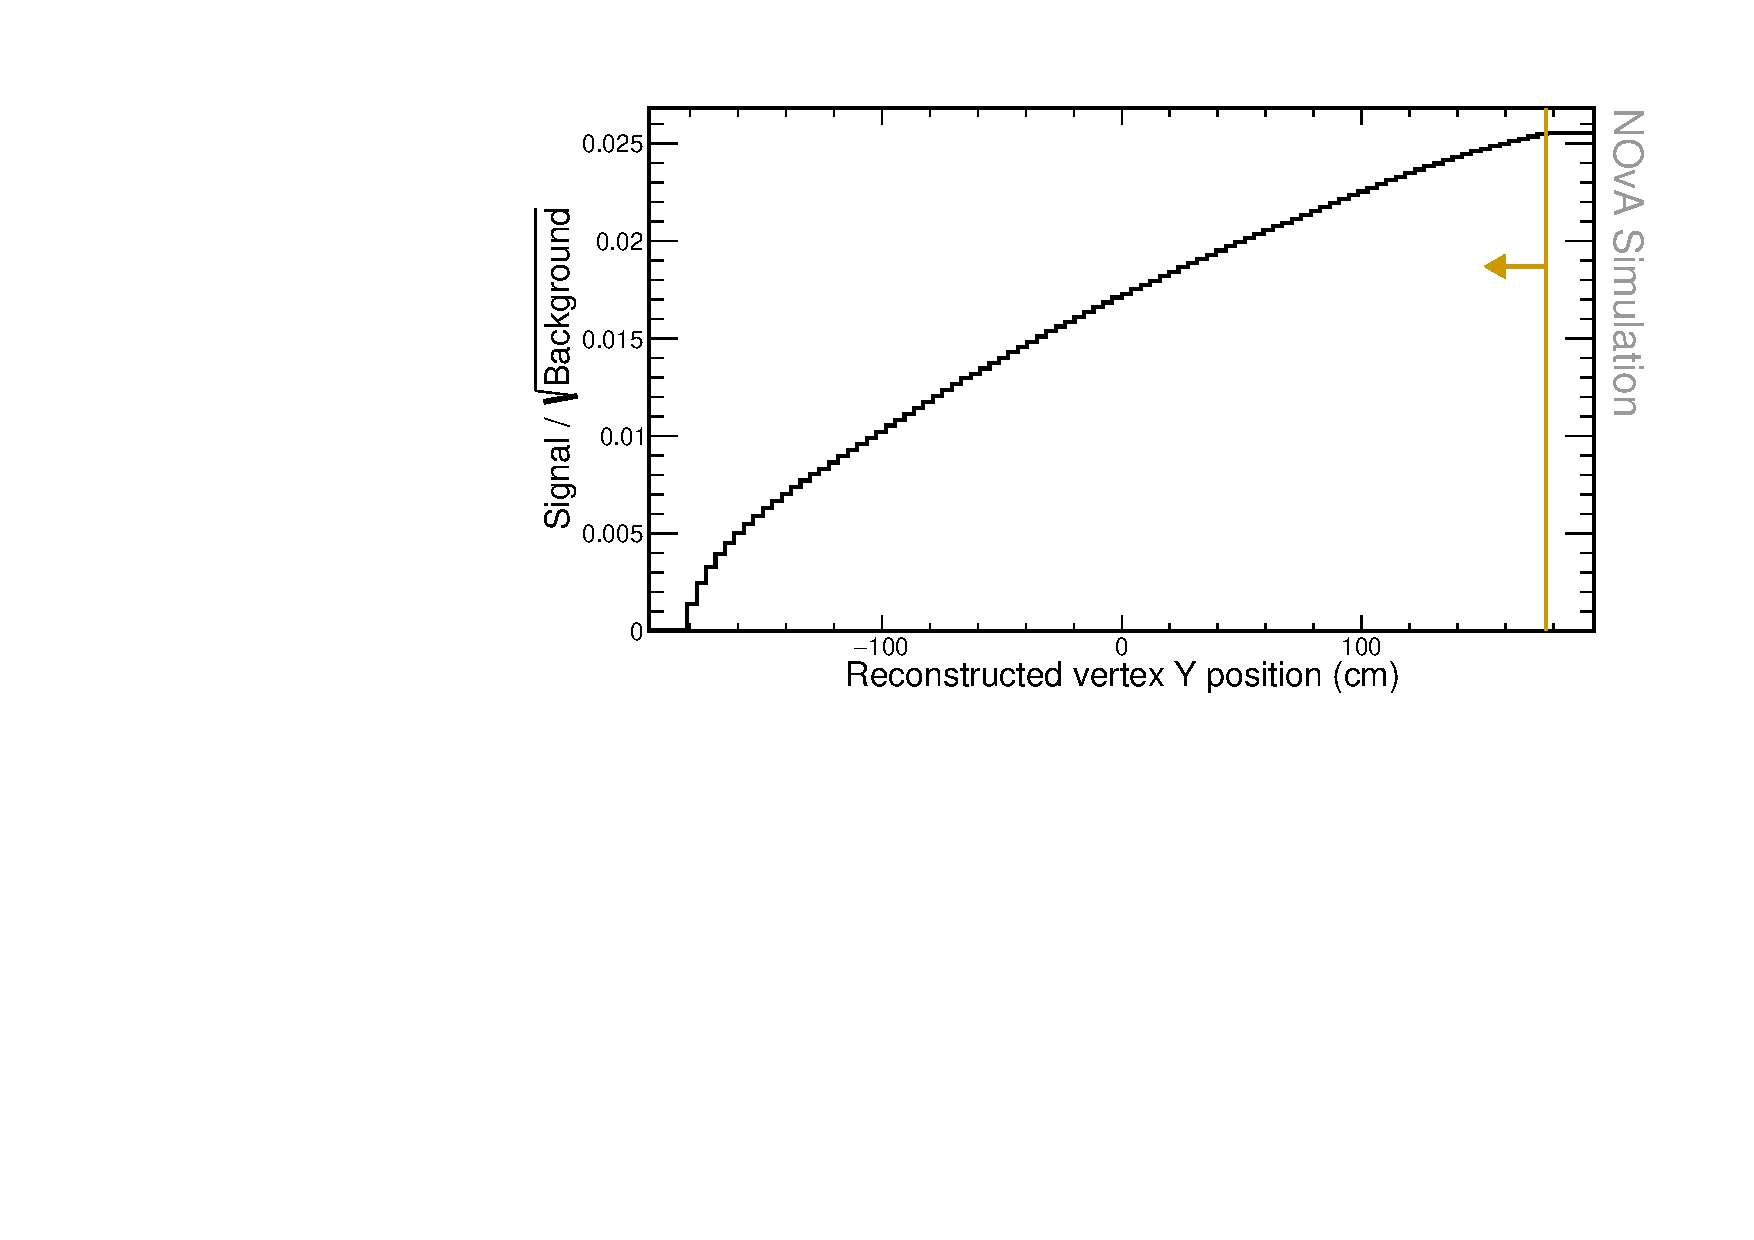
\includegraphics[width=.9\textwidth]{Plots/NuMMEventSelection/NuMM_N1Cut_vtxYActiveleft_FOMStats.pdf}
\caption[Vertex y containment cut]{Top: Relative comparison of signal (red), \acrshort{nuone} background (blue), and other background (green) events in the distribution of the y position of the reconstructed vertex. All histograms are area-normalized. Middle and bottom: Cumulative \acrshort{FOM} calculated as the number of signal events, divided by the number of background events from that bin until the end of the plot to the right (middle) or left (bottom). The reconstruction quality and pre-selection cuts were applied prior to making these plots. Additionally, vertex is required to be within the active region of the detector ($Vtx_Z<\unit[1270]{cm}$). Yellow lines show the cut values that create the fiducial volume, with arrows pointing towards the preserved events.}
\label{fig:NuMMFiducialCutY}
\end{figure}

\begin{figure}[hbtp]
\centering
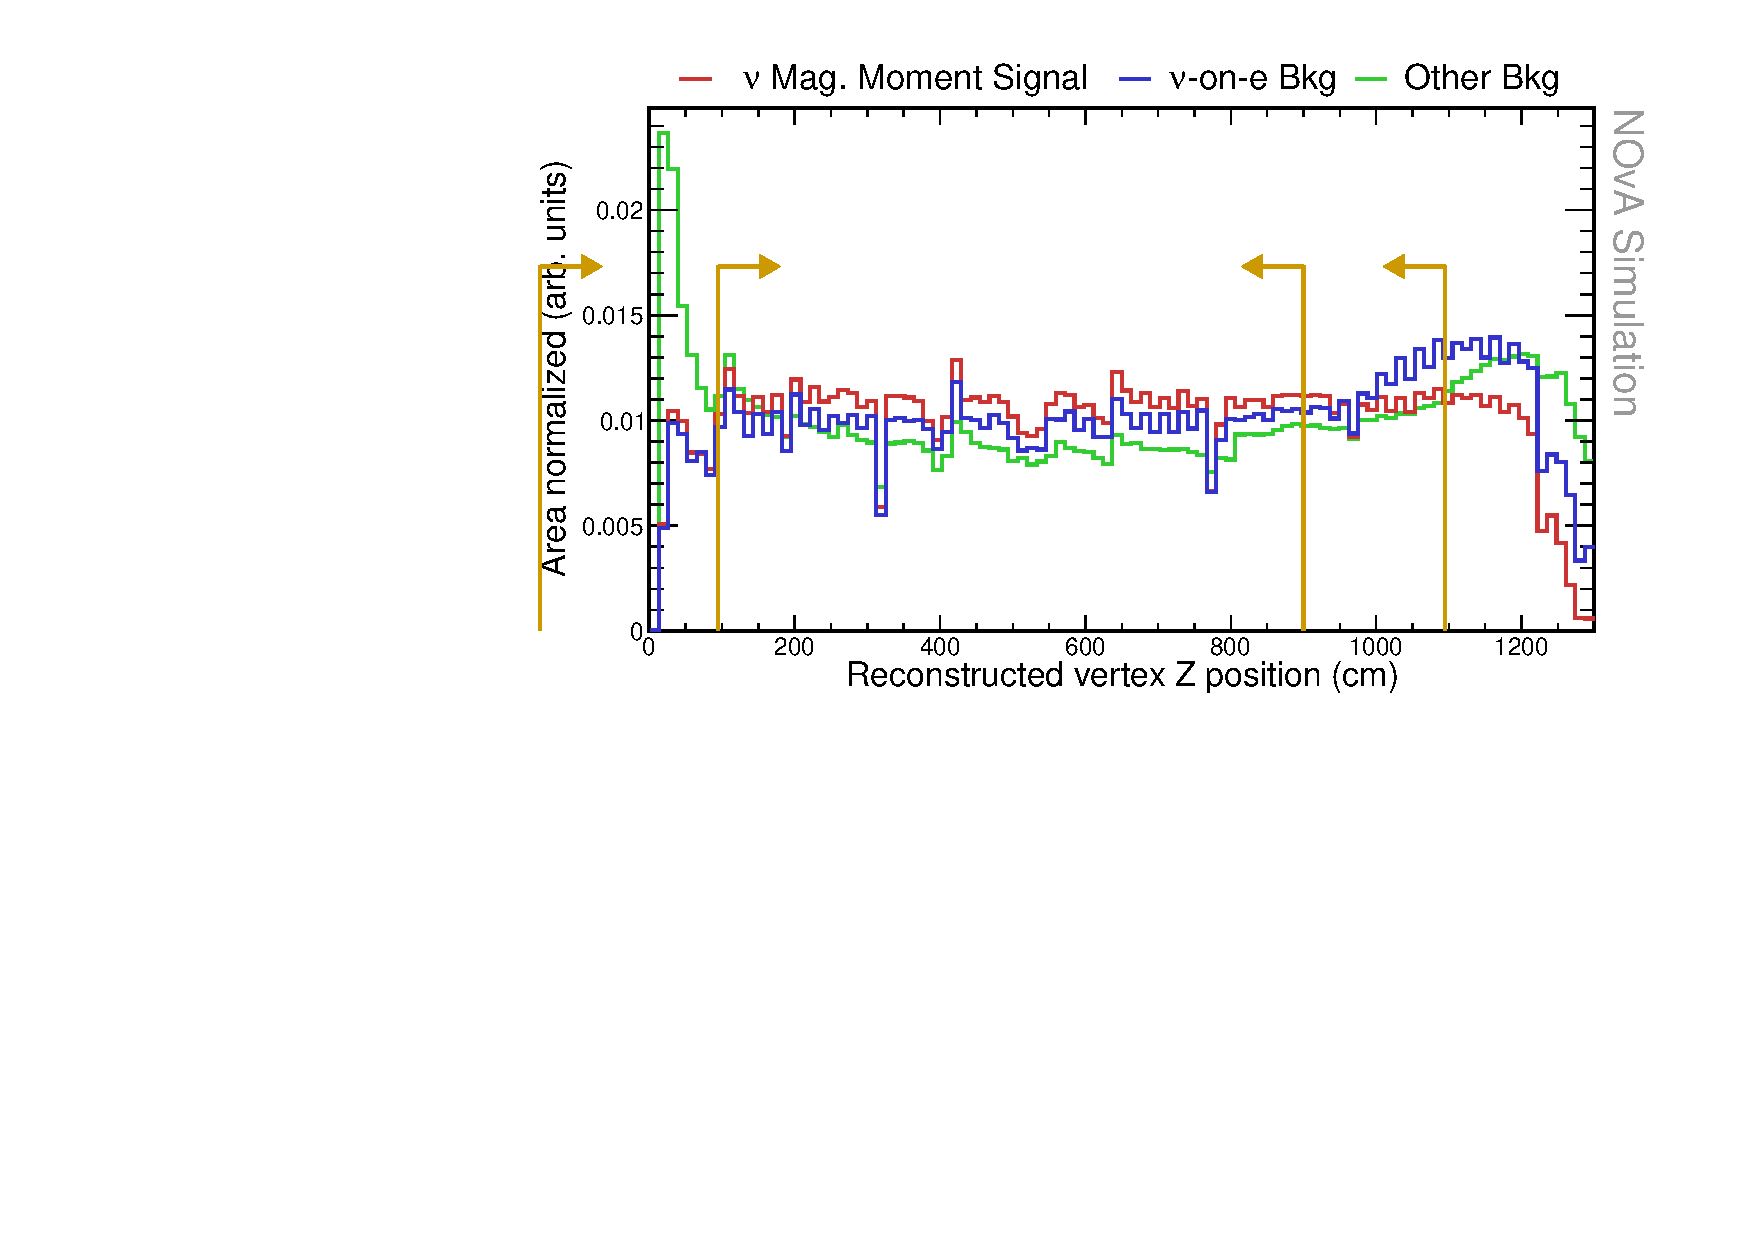
\includegraphics[width=.9\textwidth]{Plots/NuMMEventSelection/N1Cut_vtxZ.pdf}
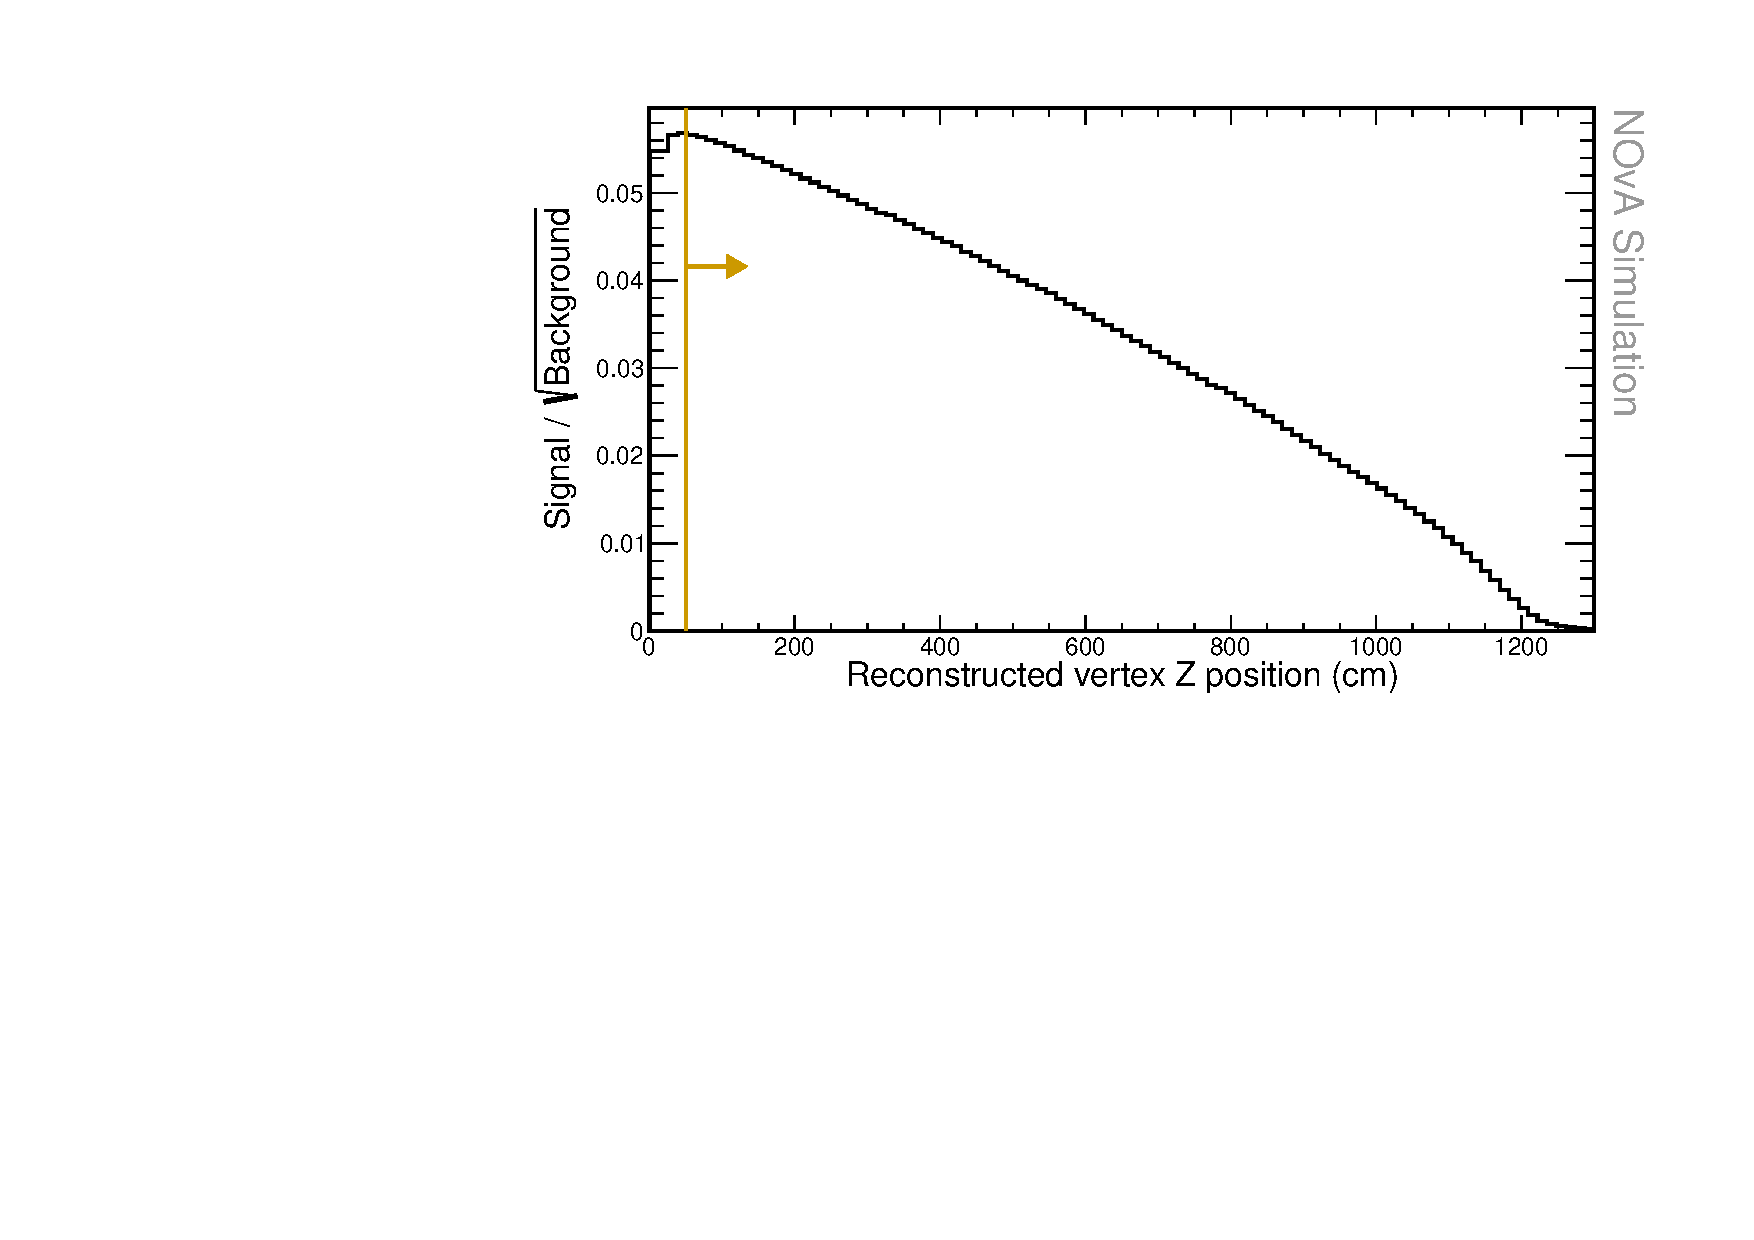
\includegraphics[width=.9\textwidth]{Plots/NuMMEventSelection/NuMM_N1Cut_vtxZright_FOMStats.pdf}
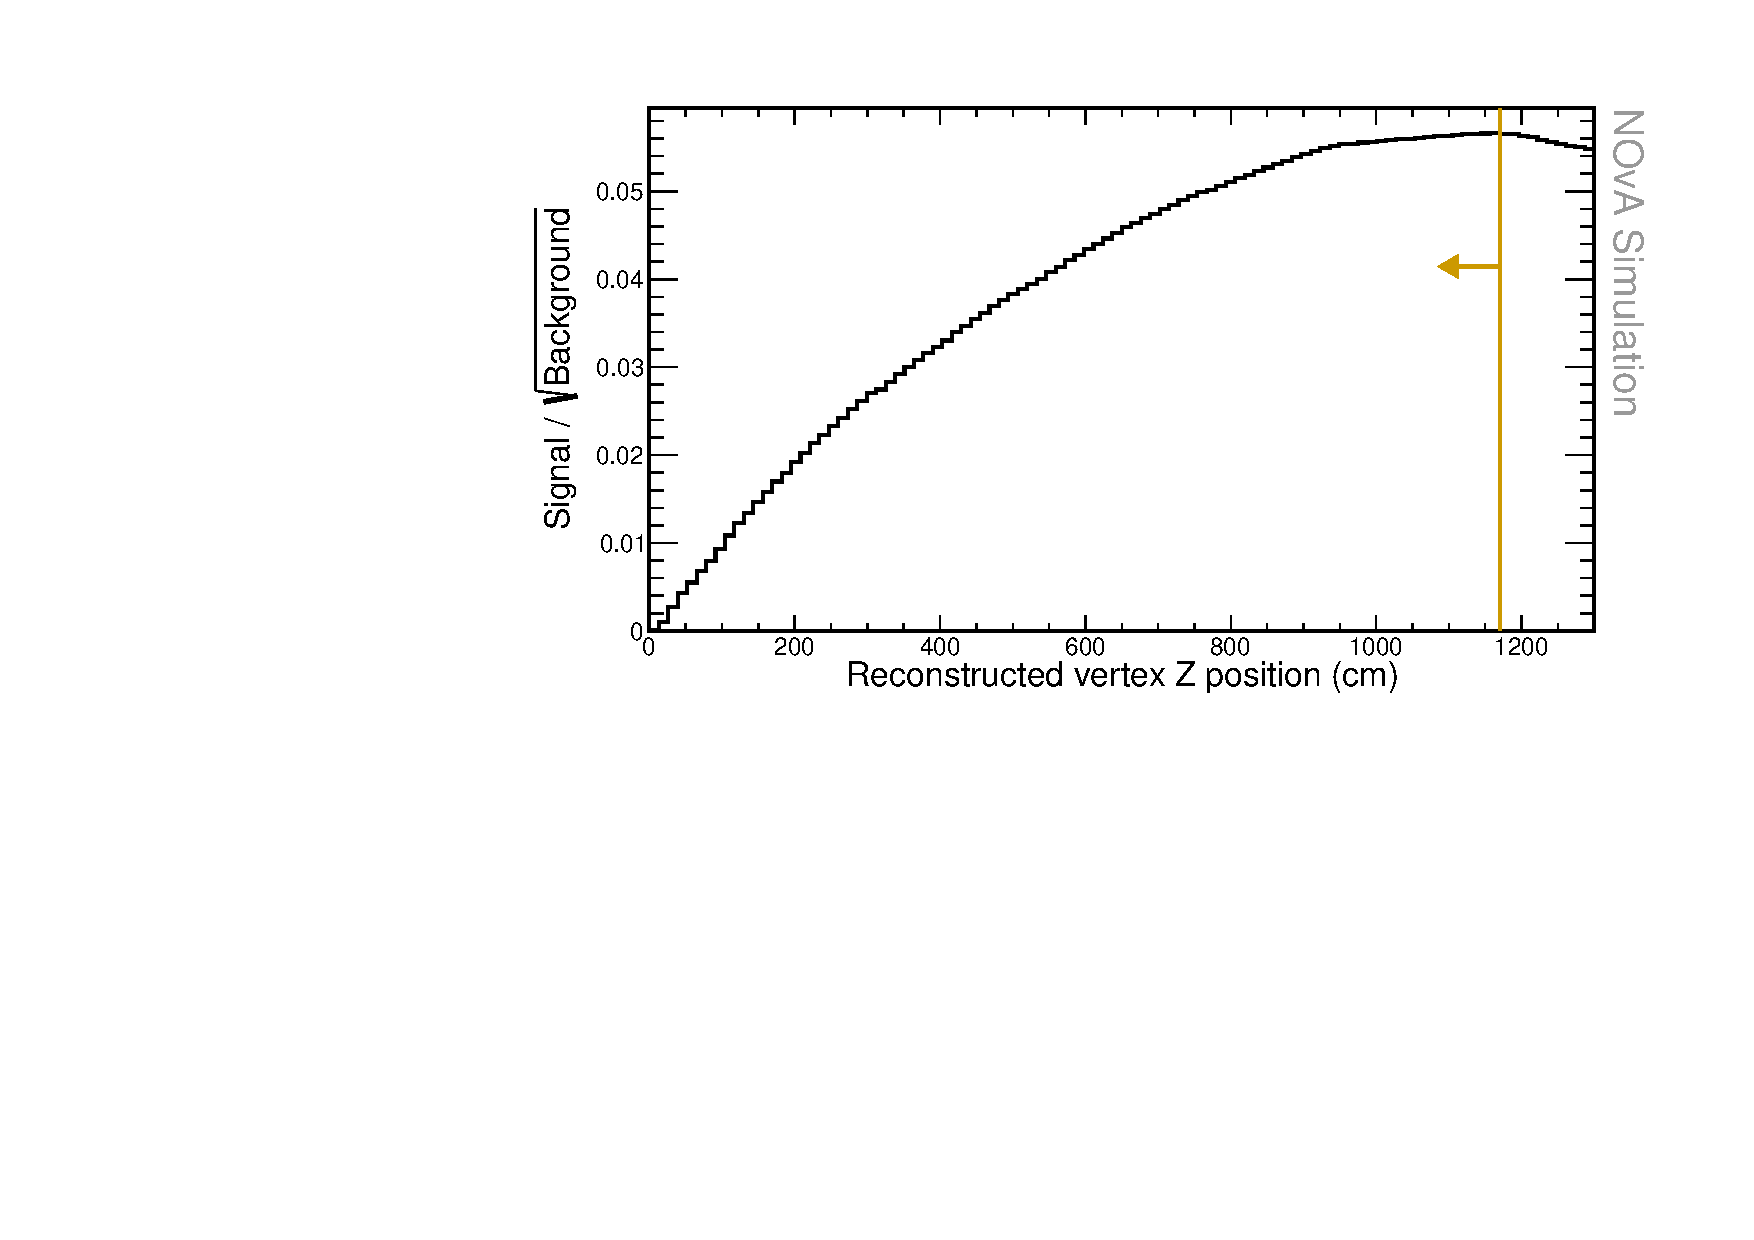
\includegraphics[width=.9\textwidth]{Plots/NuMMEventSelection/NuMM_N1Cut_vtxZleft_FOMStats.pdf}
\caption[Vertex z containment cut]{Top: Relative comparison of signal (red), \acrshort{nuone} background (blue), and other background (green) events in the distribution of the z position of the reconstructed vertex. All histograms are area-normalized. Middle and bottom: Cumulative \acrshort{FOM} calculated as the number of signal events, divided by the number of background events from that bin until the end of the plot to the right (middle) or left (bottom). The reconstruction quality and pre-selection cuts were applied prior to making these plots. Yellow lines show the cut values that create the fiducial volume, with arrows pointing towards the preserved events.}
\label{fig:NuMMFiducialCutZ}
\end{figure}

Furthermore, we constrain the extreme positions (minimum and maximum) of all the hits within the most energetic prong, which is assumed to represent the electron shower for the signal events. We apply the reconstruction quality, pre-selection and fiducial (vertex position) cuts to their distributions, shown in Fig.~\ref{fig:NuMMContainmentCutMinX}-\ref{fig:NuMMContainmentCutMaxZ}. The extreme hit positions are required to be within the following volume: 
\begin{align}
\unit[-175]{cm}<\textsf{min}_X,& \textsf{max}_X<\unit[175]{cm},\\
\unit[-175]{cm}<\textsf{min}_Y,& \textsf{max}_Y<\unit[175]{cm},\\
\unit[105]{cm}<\textsf{min}_Z,& \textsf{max}_Z<\unit[1270]{cm}.
\end{align}

\begin{figure}[hbtp]
\centering
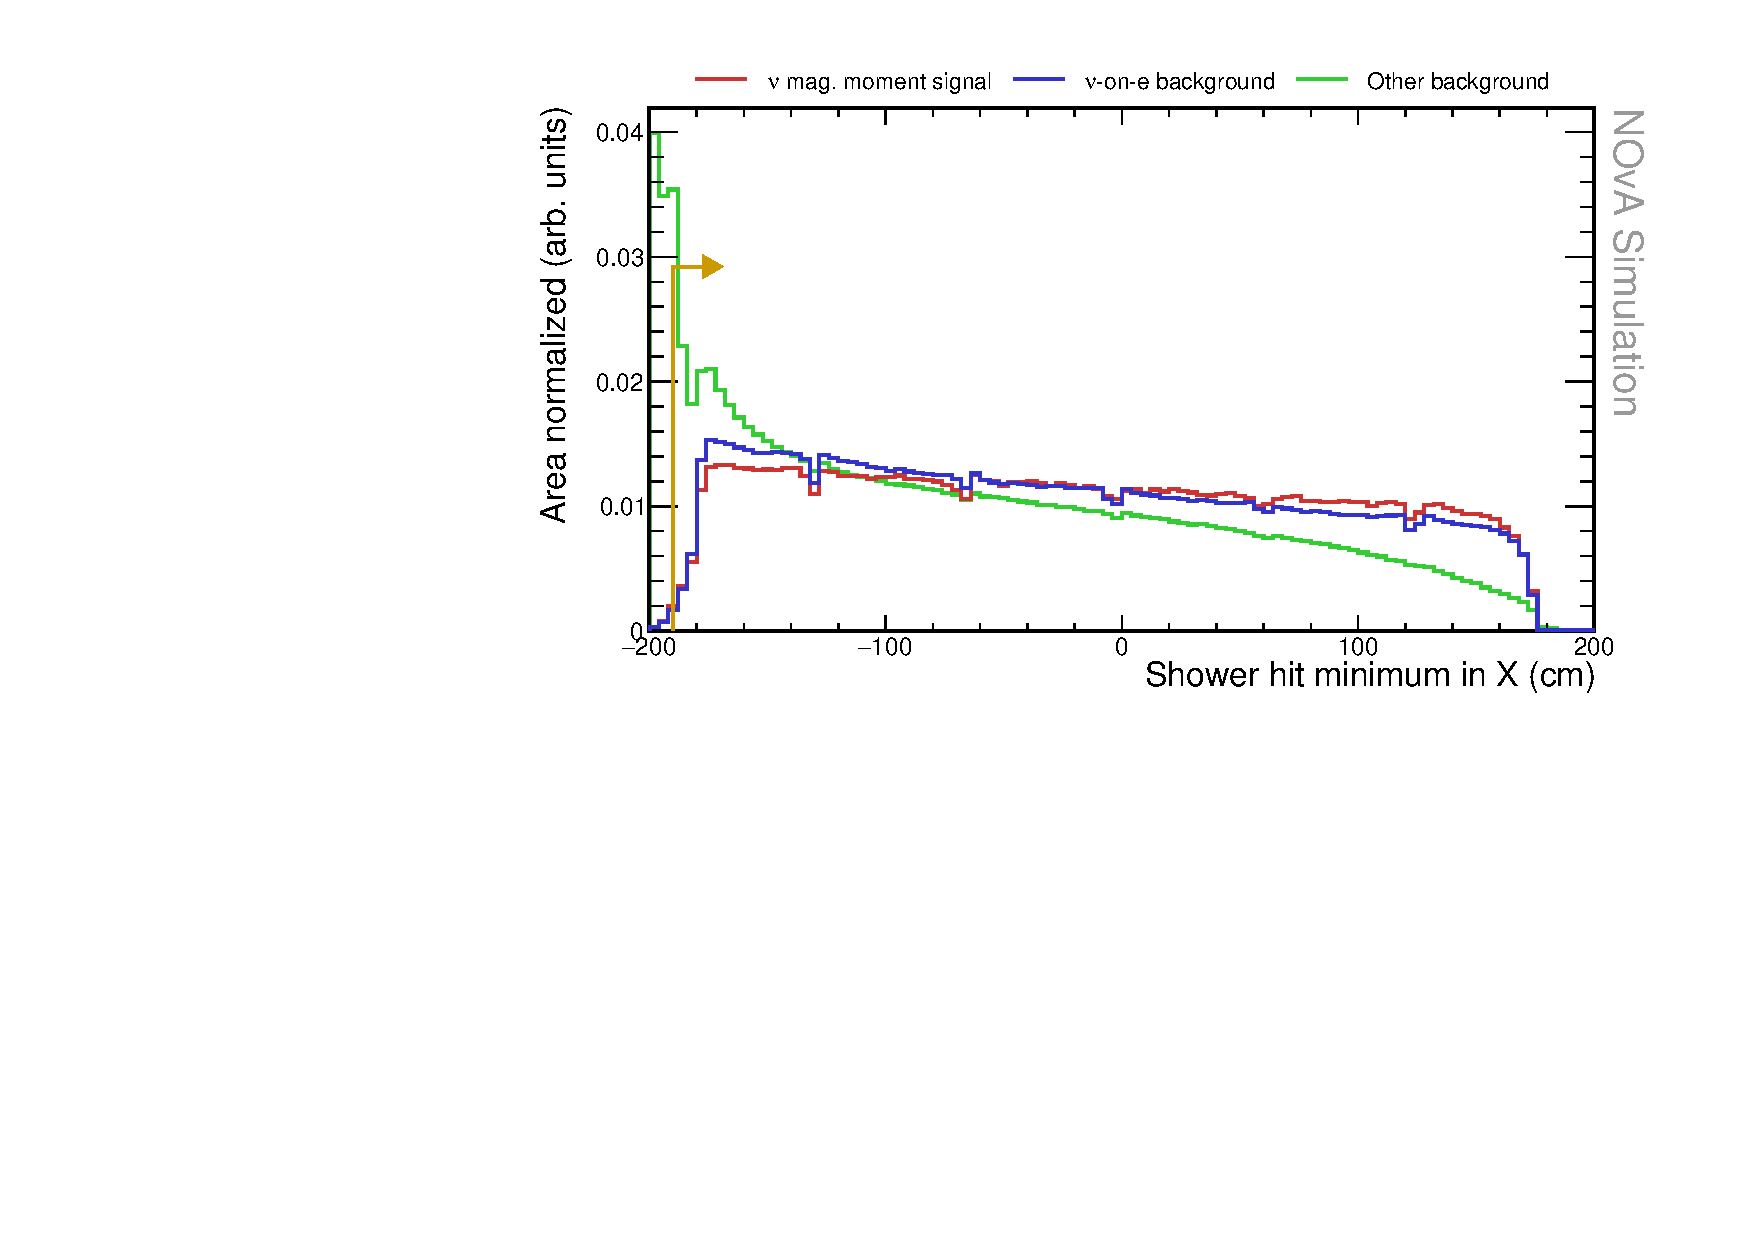
\includegraphics[width=.9\textwidth]{Plots/NuMMEventSelection/N1Cut_minX.pdf}
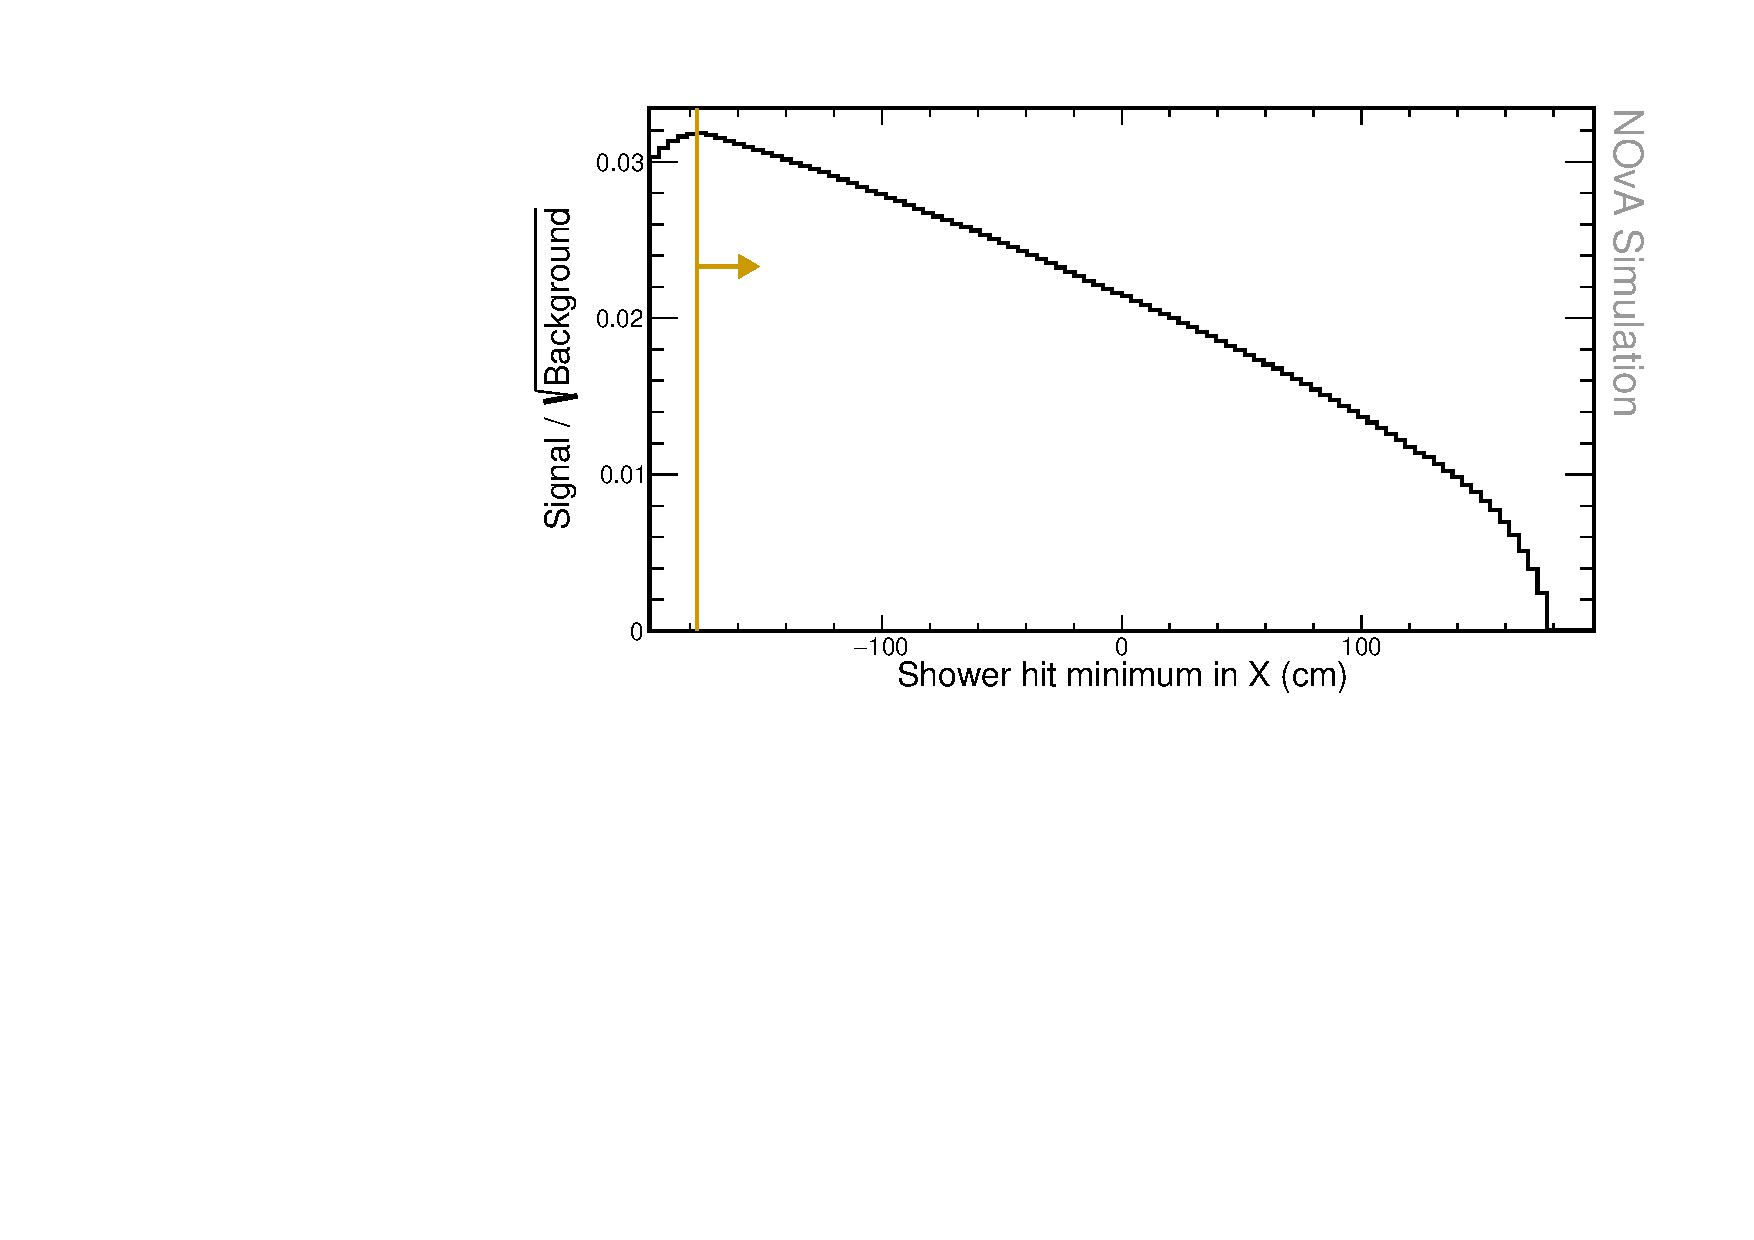
\includegraphics[width=.9\textwidth]{Plots/NuMMEventSelection/NuMM_N1Cut_minXright_FOMStats.pdf}
\caption[Hit minimum x containment cut]{Top: Relative comparison of signal (red), \acrshort{nuone} background (blue), and other background (green) events in the distribution of the minimum hit position of the most energetic prong along the x axis. All histograms are area-normalized. Bottom: Cumulative \acrshort{FOM} calculated as the number of signal events, divided by the number of background events from that bin until the end of the plot in the direction of the yellow arrow. The reconstruction quality, pre-selection and fiducial cuts were applied prior to making these plots. Yellow lines show the cut values that create the containment volume, with arrows pointing towards the preserved events.}
\label{fig:NuMMContainmentCutMinX}
\end{figure}

\begin{figure}[hbtp]
\centering
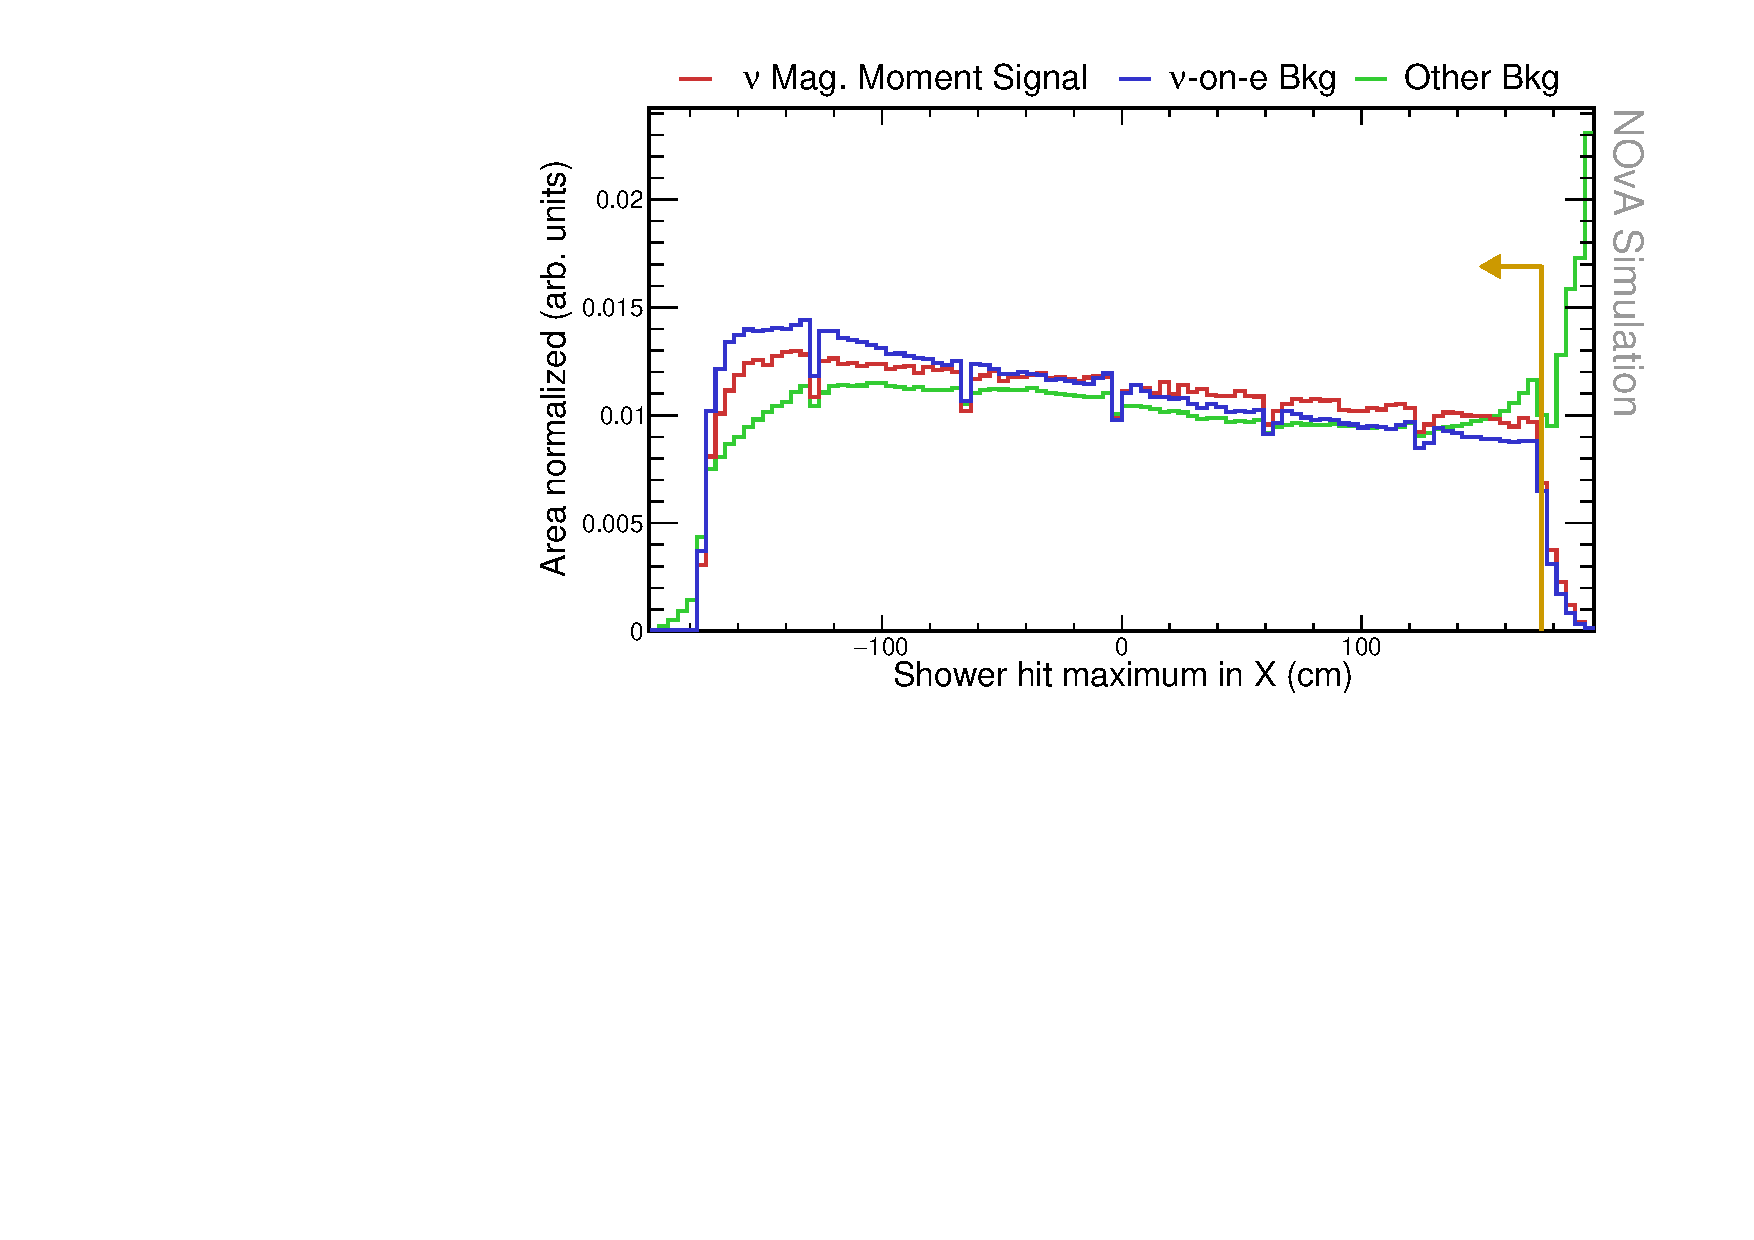
\includegraphics[width=.9\textwidth]{Plots/NuMMEventSelection/N1Cut_maxX.pdf}
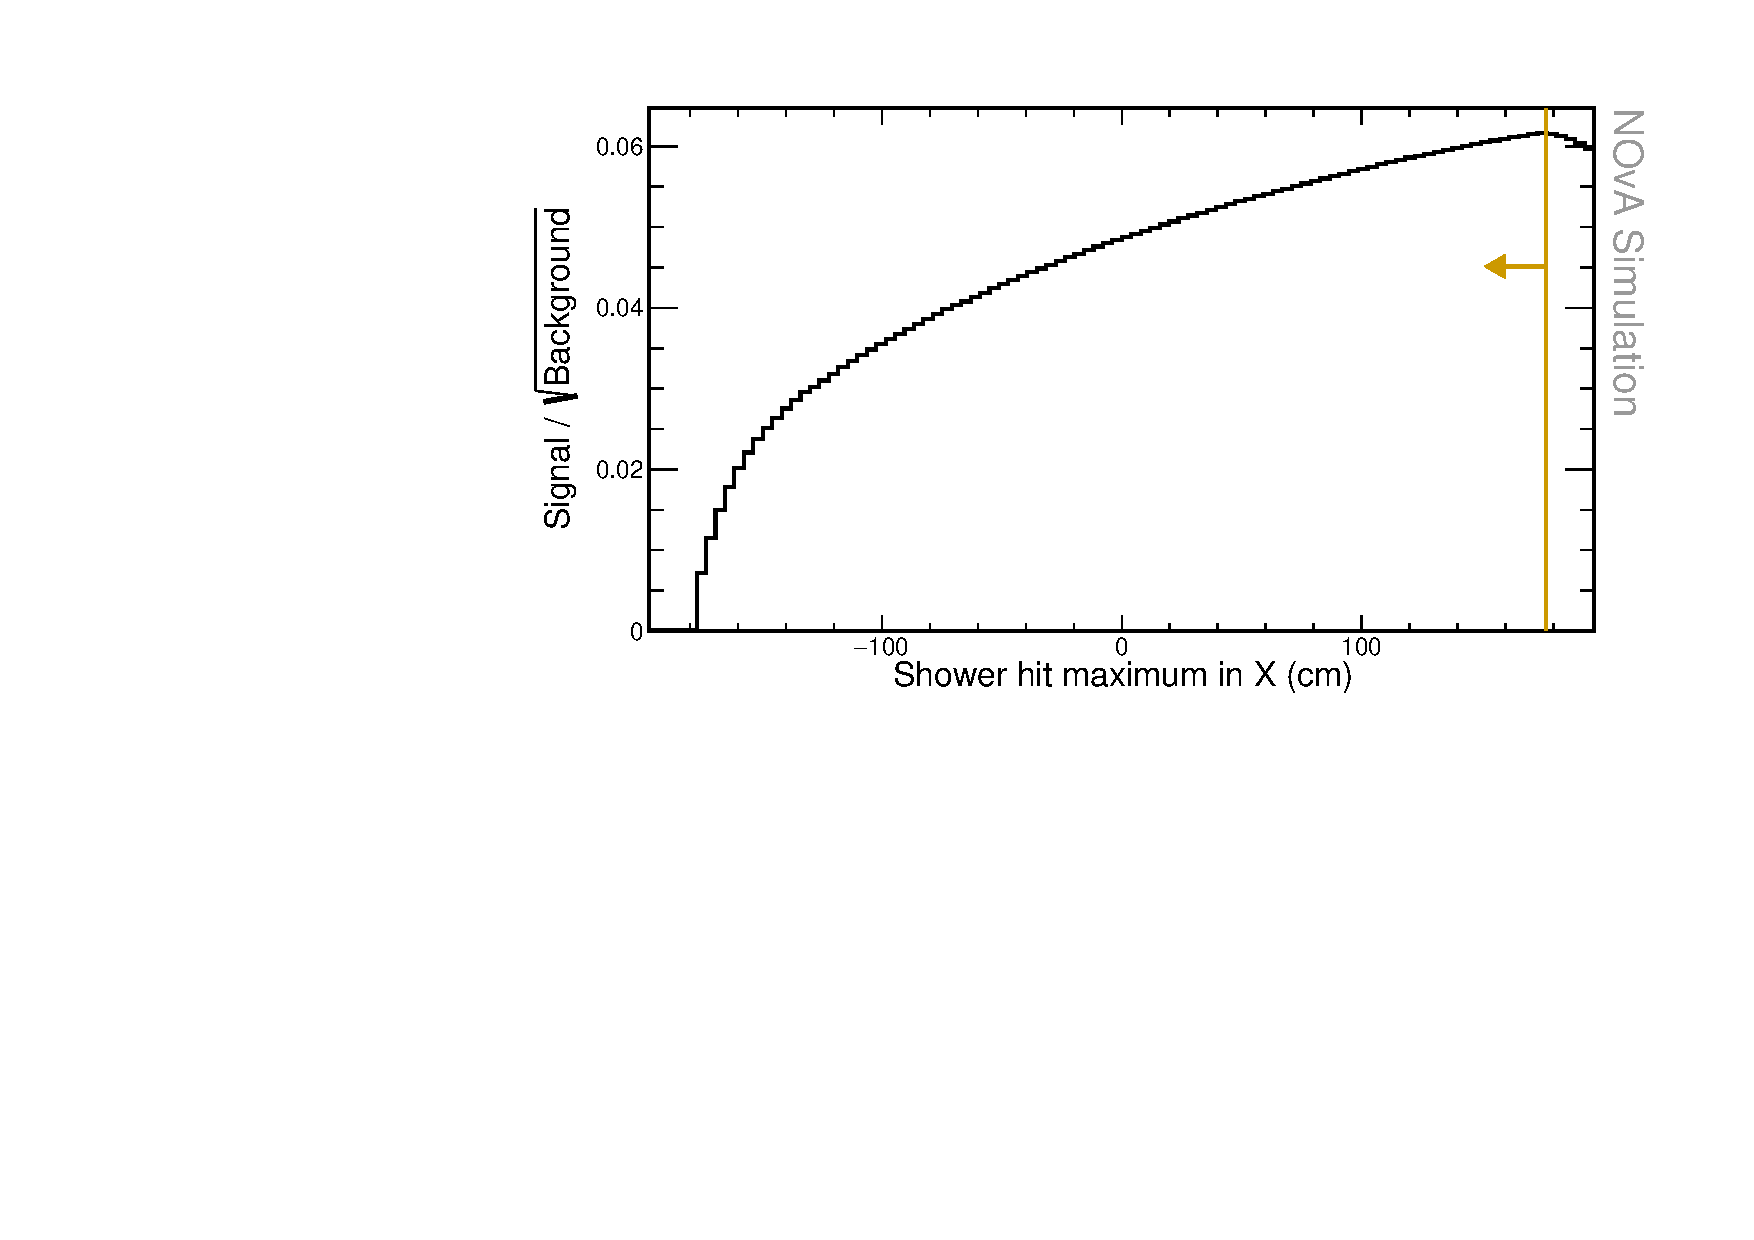
\includegraphics[width=.9\textwidth]{Plots/NuMMEventSelection/NuMM_N1Cut_maxXleft_FOMStats}
\caption[Hit maximum x containment cut]{Top: Relative comparison of signal (red), \acrshort{nuone} background (blue), and other background (green) events in the distribution of the maximum hit position of the most energetic prong along the x axis. All histograms are area-normalized. Bottom: Cumulative \acrshort{FOM} calculated as the number of signal events, divided by the number of background events from that bin until the end of the plot in the direction of the yellow arrow. The reconstruction quality, pre-selection and fiducial cuts were applied prior to making these plots. Yellow lines show the cut values that create the containment volume, with arrows pointing towards the preserved events.}
\label{fig:NuMMContainmentCutMaxX}
\end{figure}

\begin{figure}[hbtp]
\centering
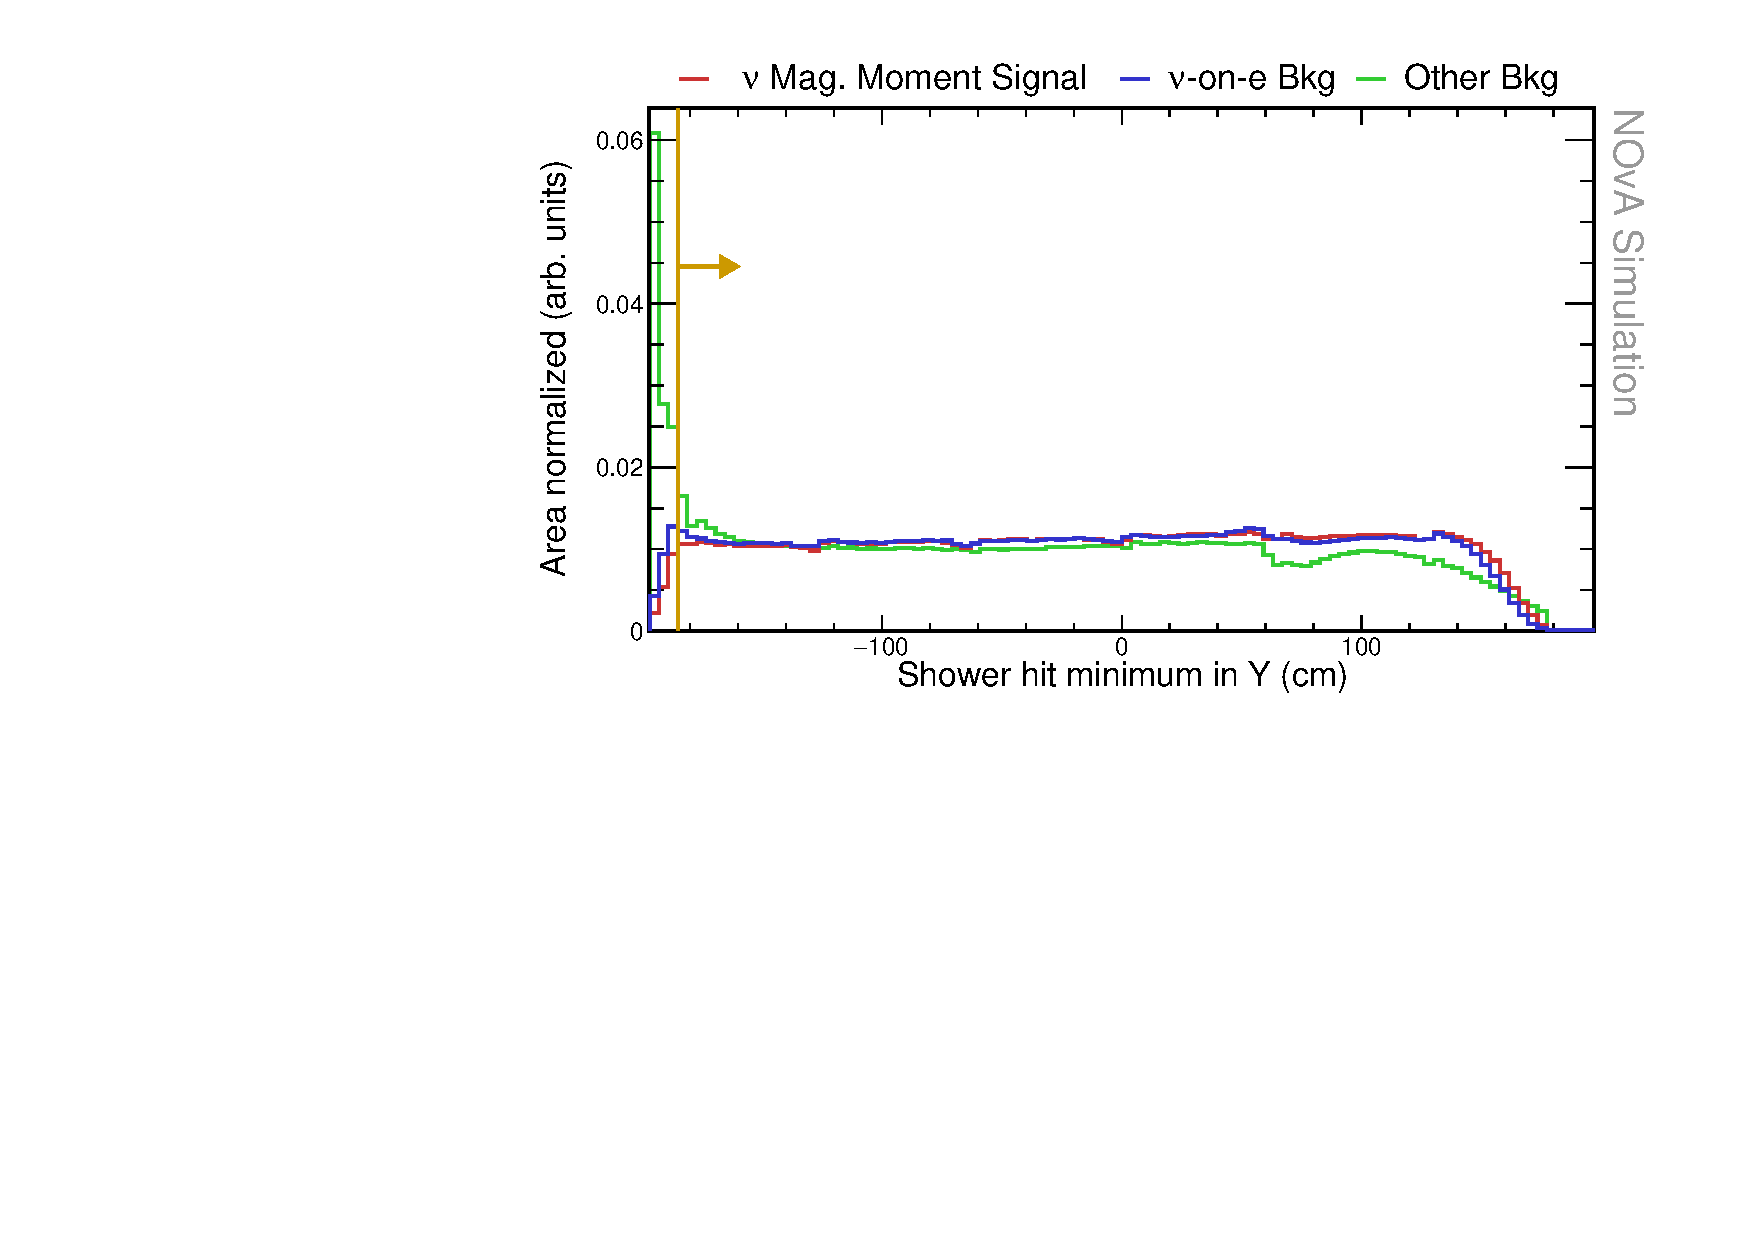
\includegraphics[width=.9\textwidth]{Plots/NuMMEventSelection/N1Cut_minY.pdf}
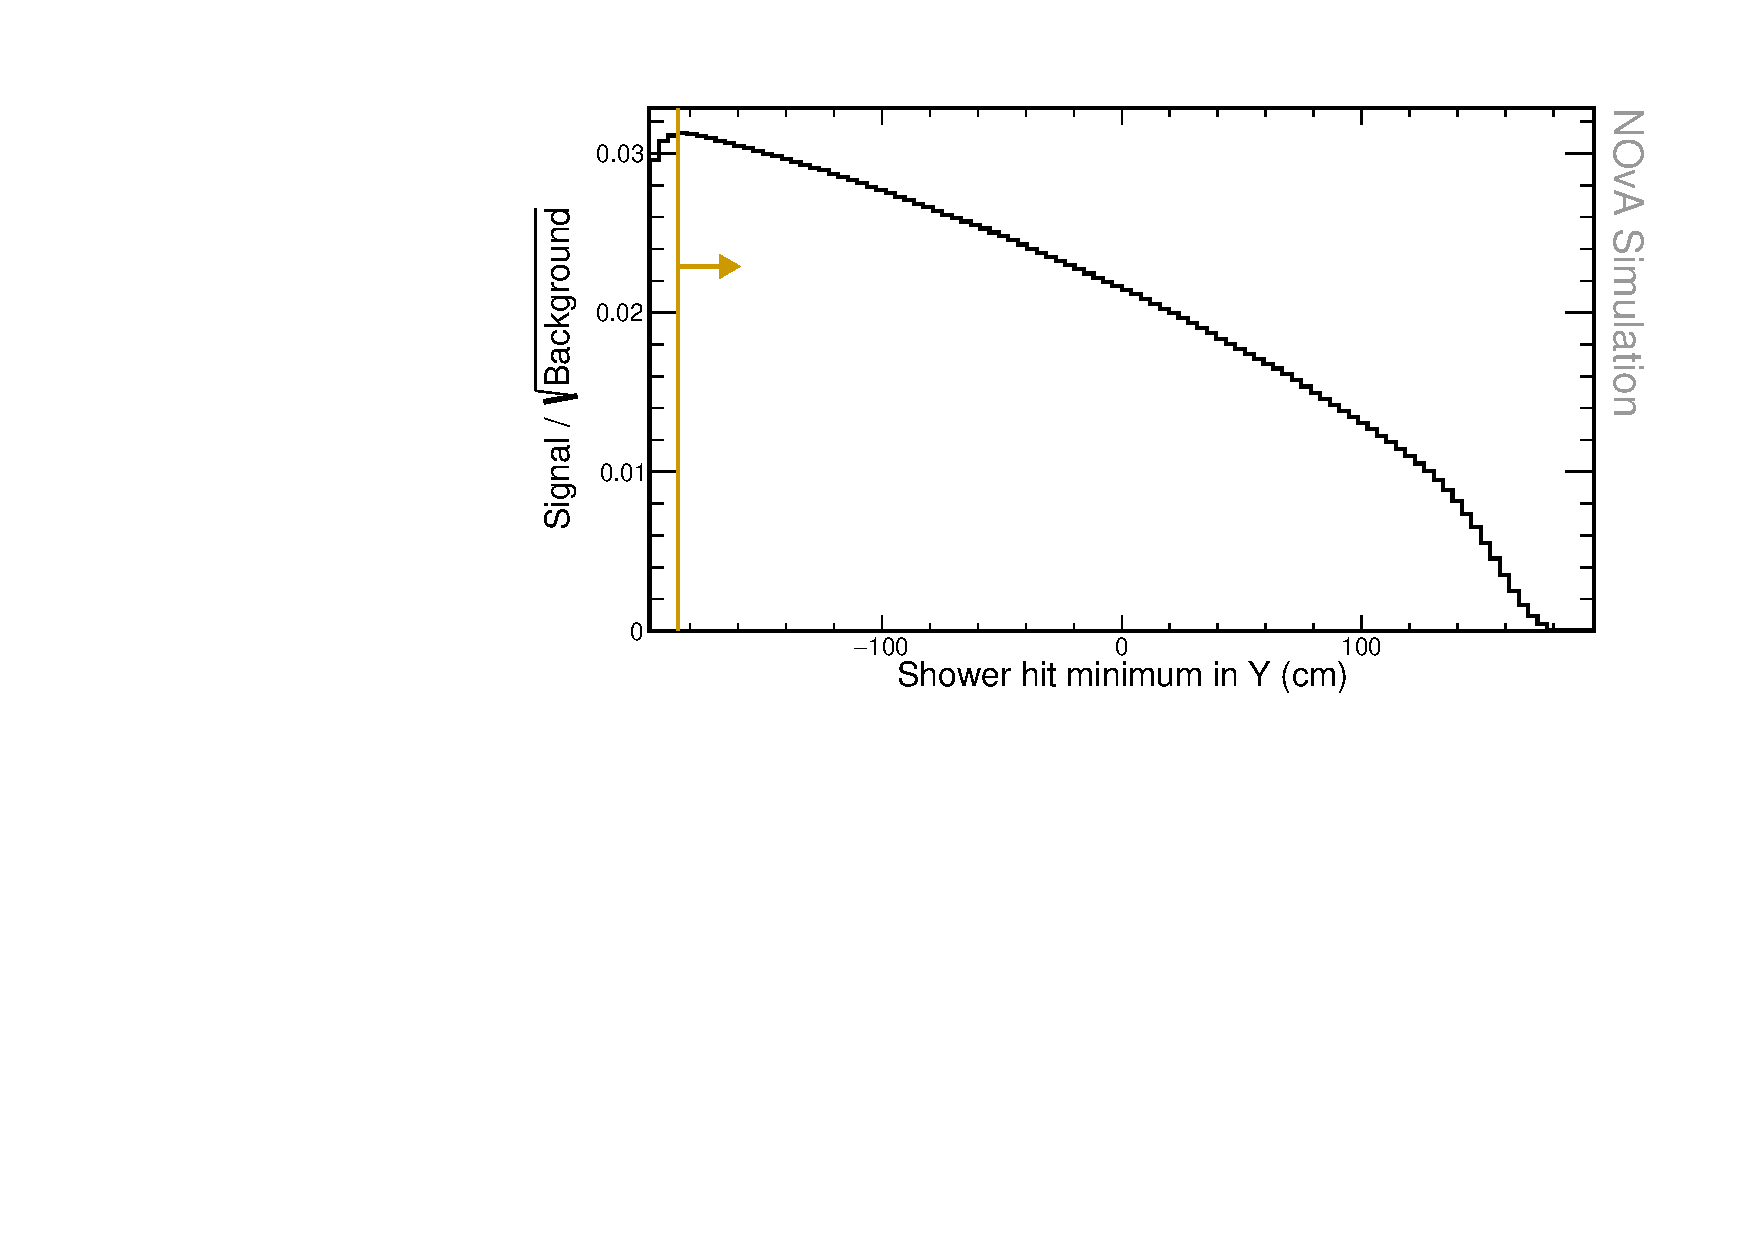
\includegraphics[width=.9\textwidth]{Plots/NuMMEventSelection/NuMM_N1Cut_minYright_FOMStats.pdf}
\caption[Hit minimum y containment cut]{Top: Relative comparison of signal (red), \acrshort{nuone} background (blue), and other background (green) events in the distribution of the minimum hit position of the most energetic prong along the y axis. All histograms are area-normalized. Bottom: Cumulative \acrshort{FOM} calculated as the number of signal events, divided by the number of background events from that bin until the end of the plot in the direction of the yellow arrow. The reconstruction quality, pre-selection and fiducial cuts were applied prior to making these plots. Yellow lines show the cut values that create the containment volume, with arrows pointing towards the preserved events.}
\label{fig:NuMMContainmentCutMinY}
\end{figure}

\begin{figure}[hbtp]
\centering
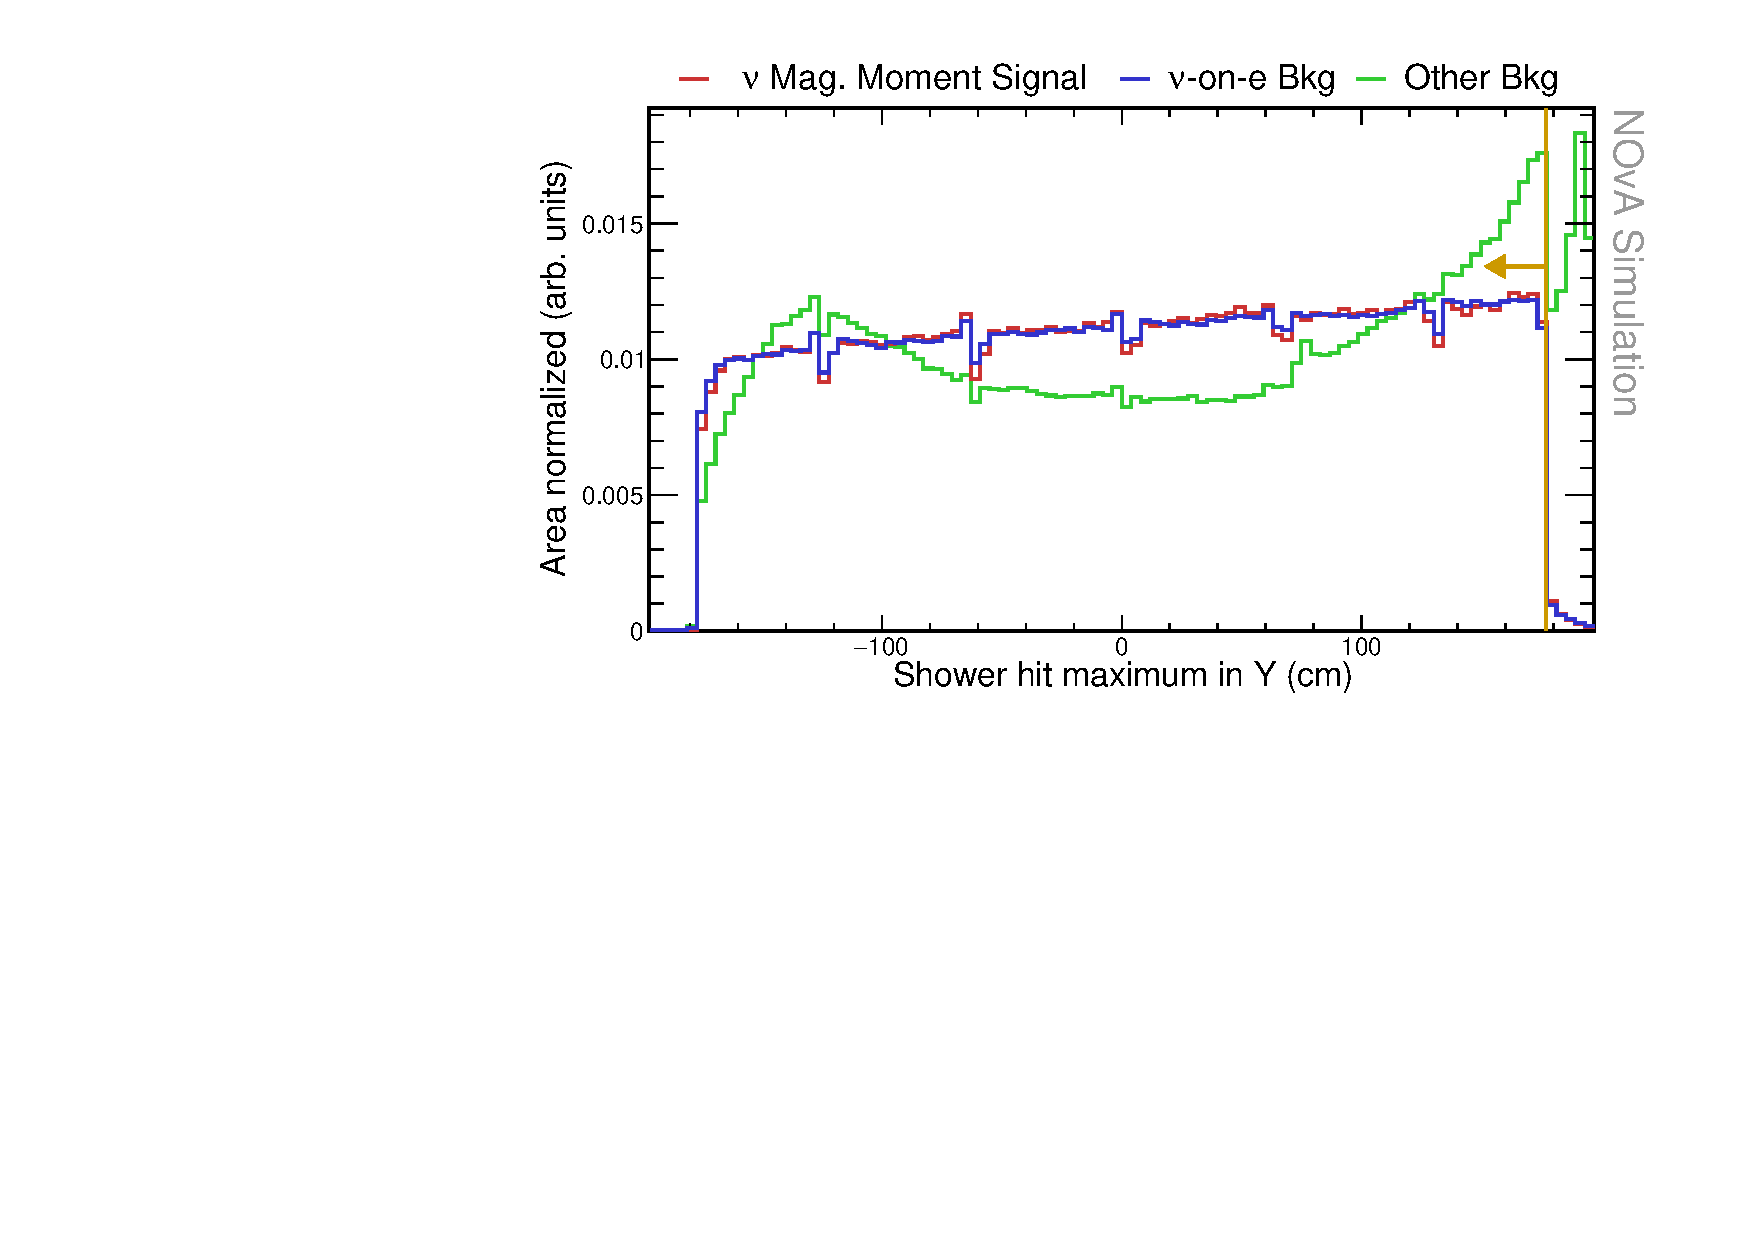
\includegraphics[width=.9\textwidth]{Plots/NuMMEventSelection/N1Cut_maxY.pdf}
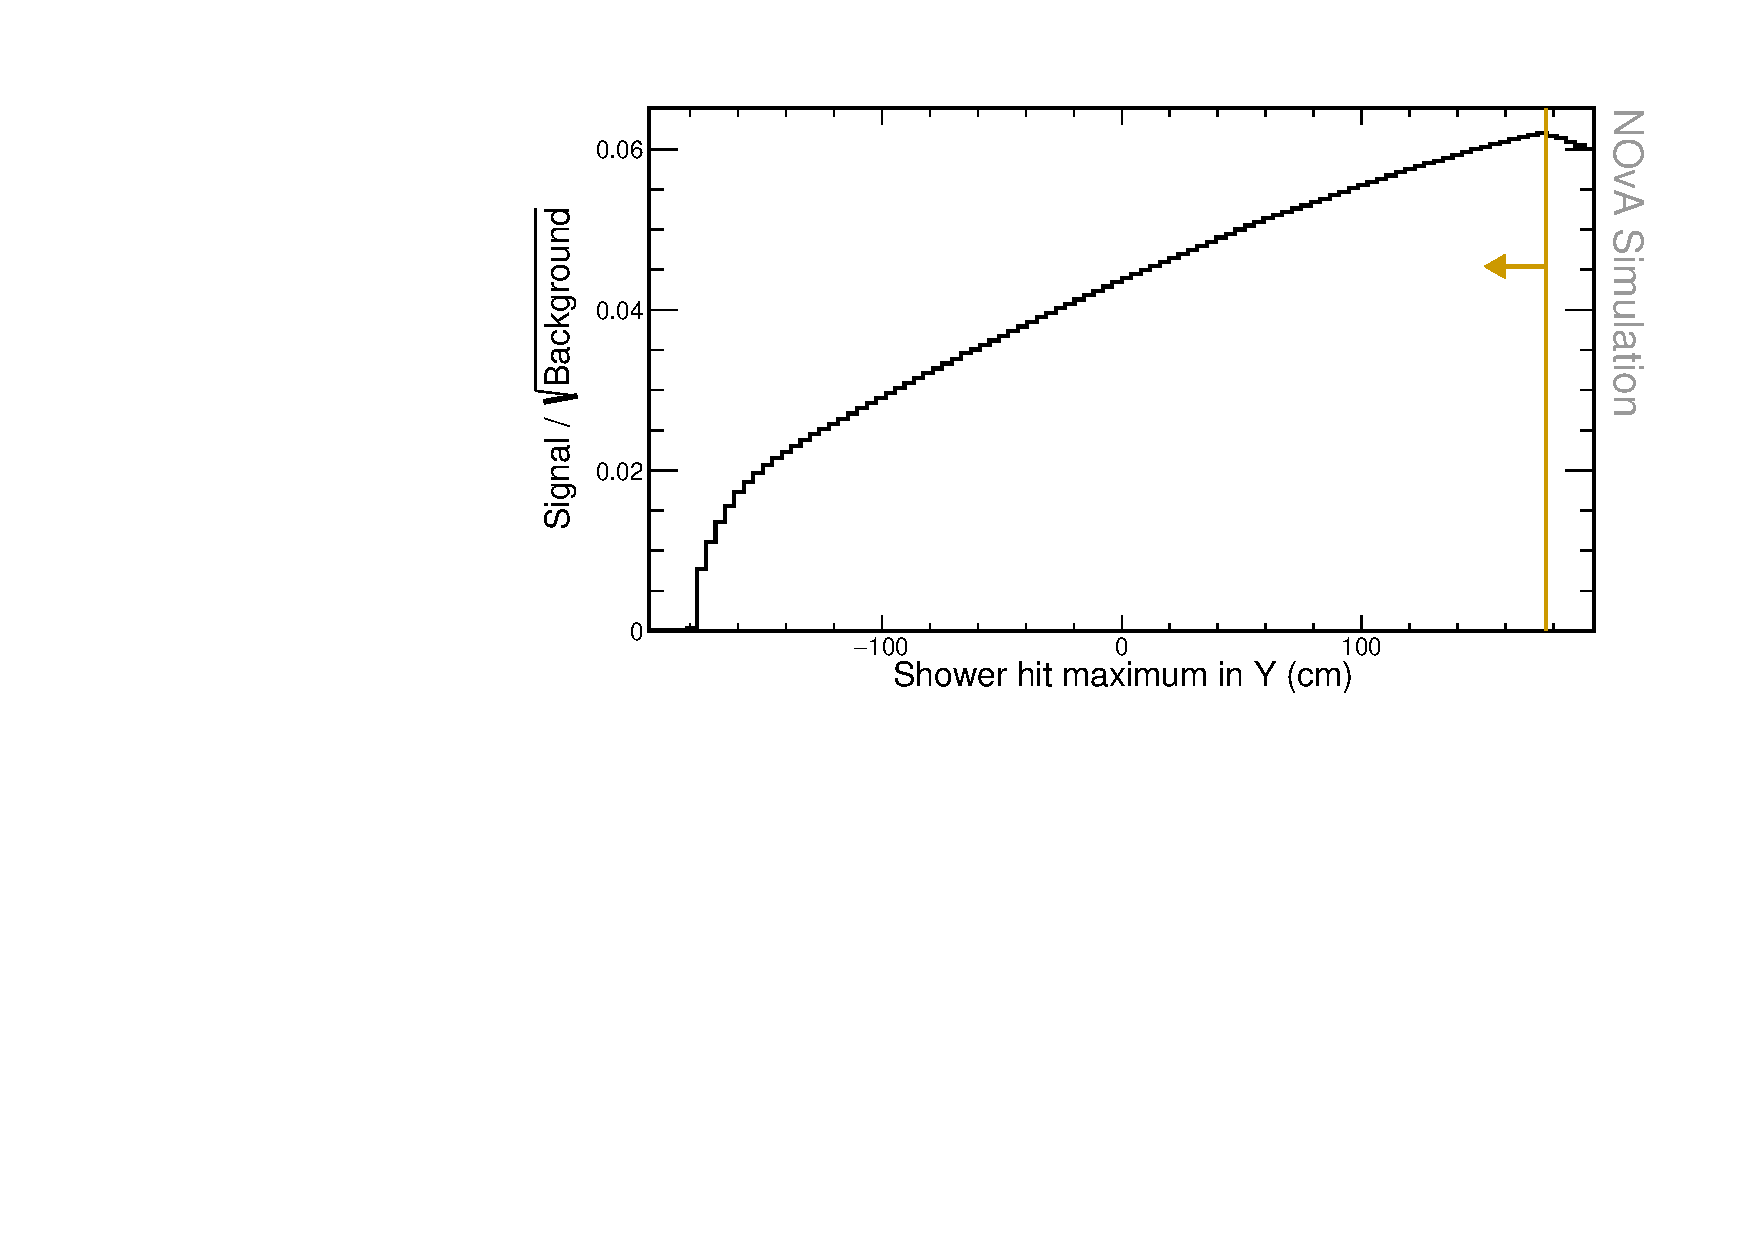
\includegraphics[width=.9\textwidth]{Plots/NuMMEventSelection/NuMM_N1Cut_maxYleft_FOMStats}
\caption[Hit maximum y containment cut]{Top: Relative comparison of signal (red), \acrshort{nuone} background (blue), and other background (green) events in the distribution of the maximum hit position of the most energetic prong along the y axis. All histograms are area-normalized. Bottom: Cumulative \acrshort{FOM} calculated as the number of signal events, divided by the number of background events from that bin until the end of the plot in the direction of the yellow arrow. The reconstruction quality, pre-selection and fiducial cuts were applied prior to making these plots. Yellow lines show the cut values that create the containment volume, with arrows pointing towards the preserved events.}
\label{fig:NuMMContainmentCutMaxY}
\end{figure}

\begin{figure}[hbtp]
\centering
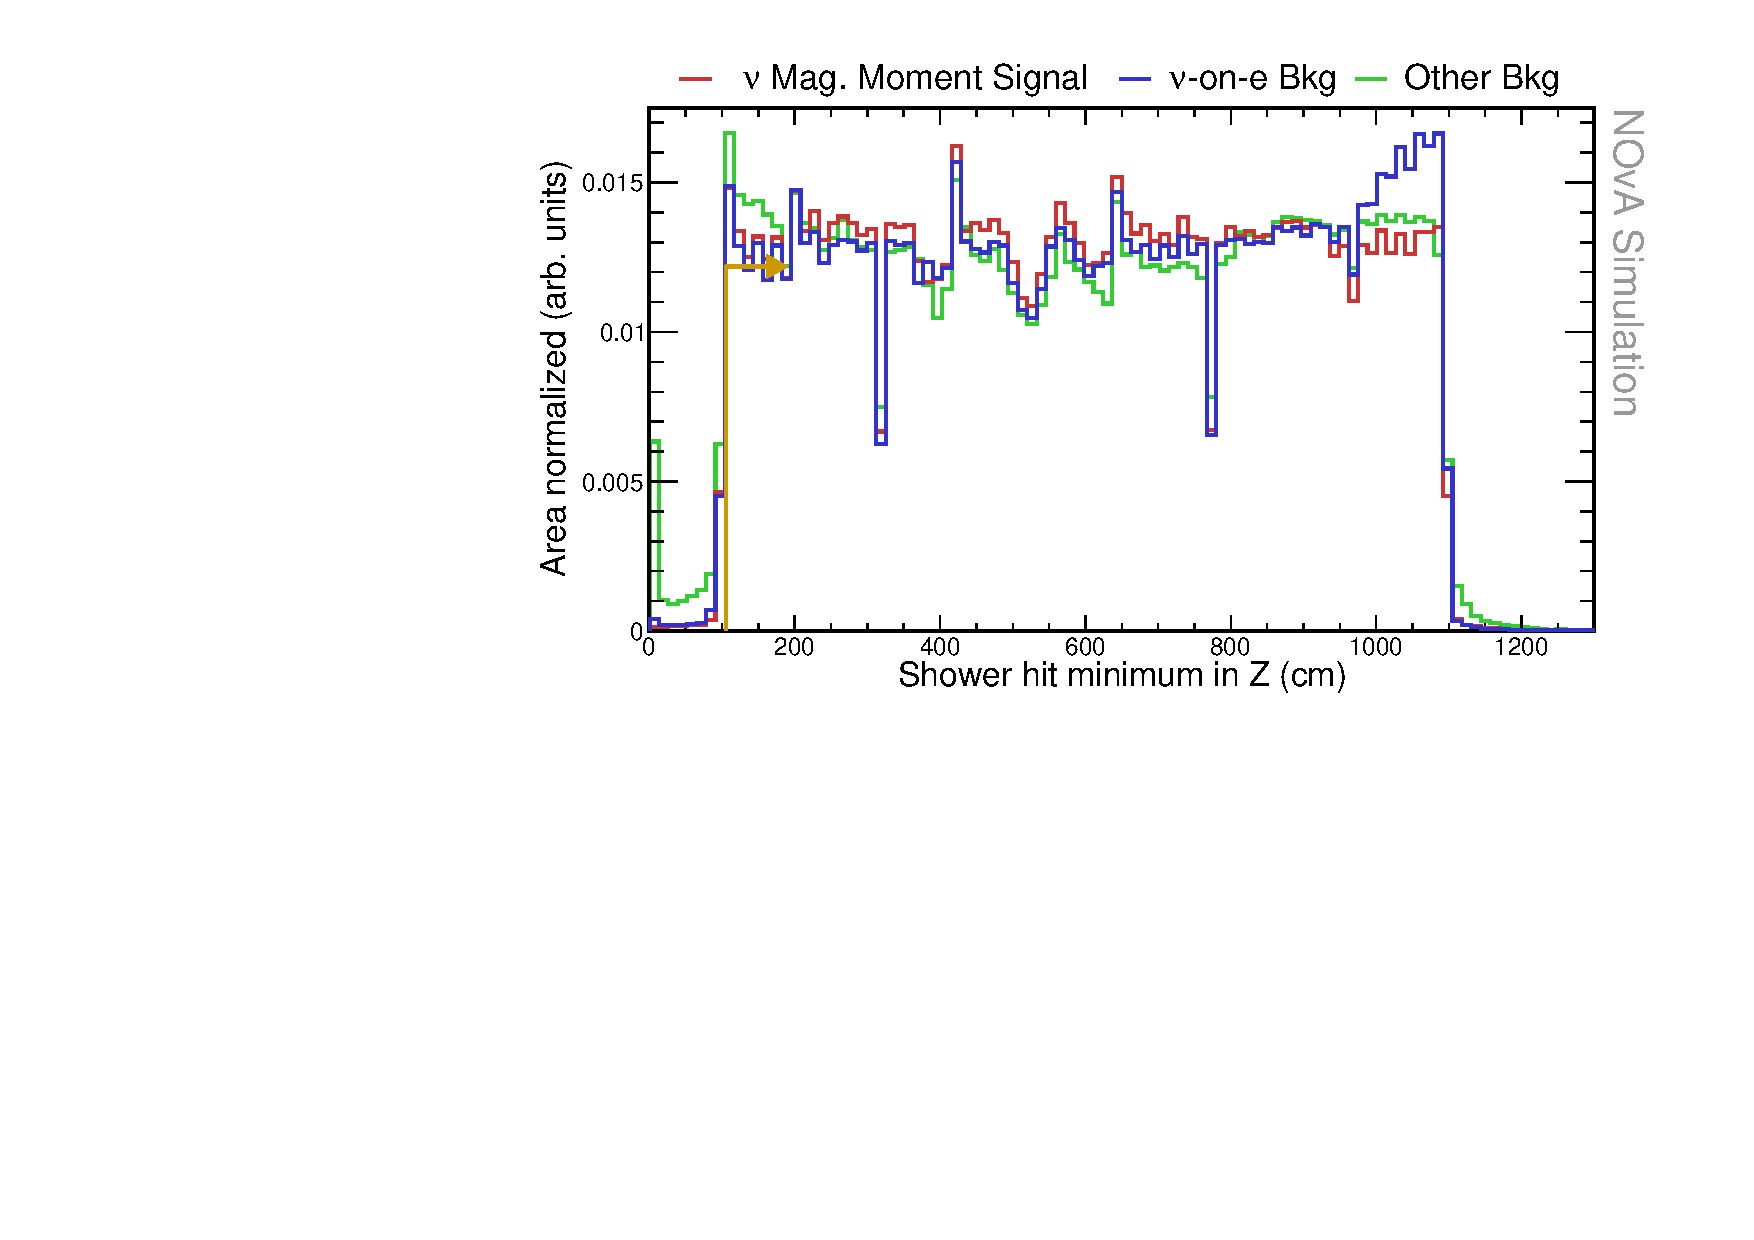
\includegraphics[width=.9\textwidth]{Plots/NuMMEventSelection/N1Cut_minZ.pdf}
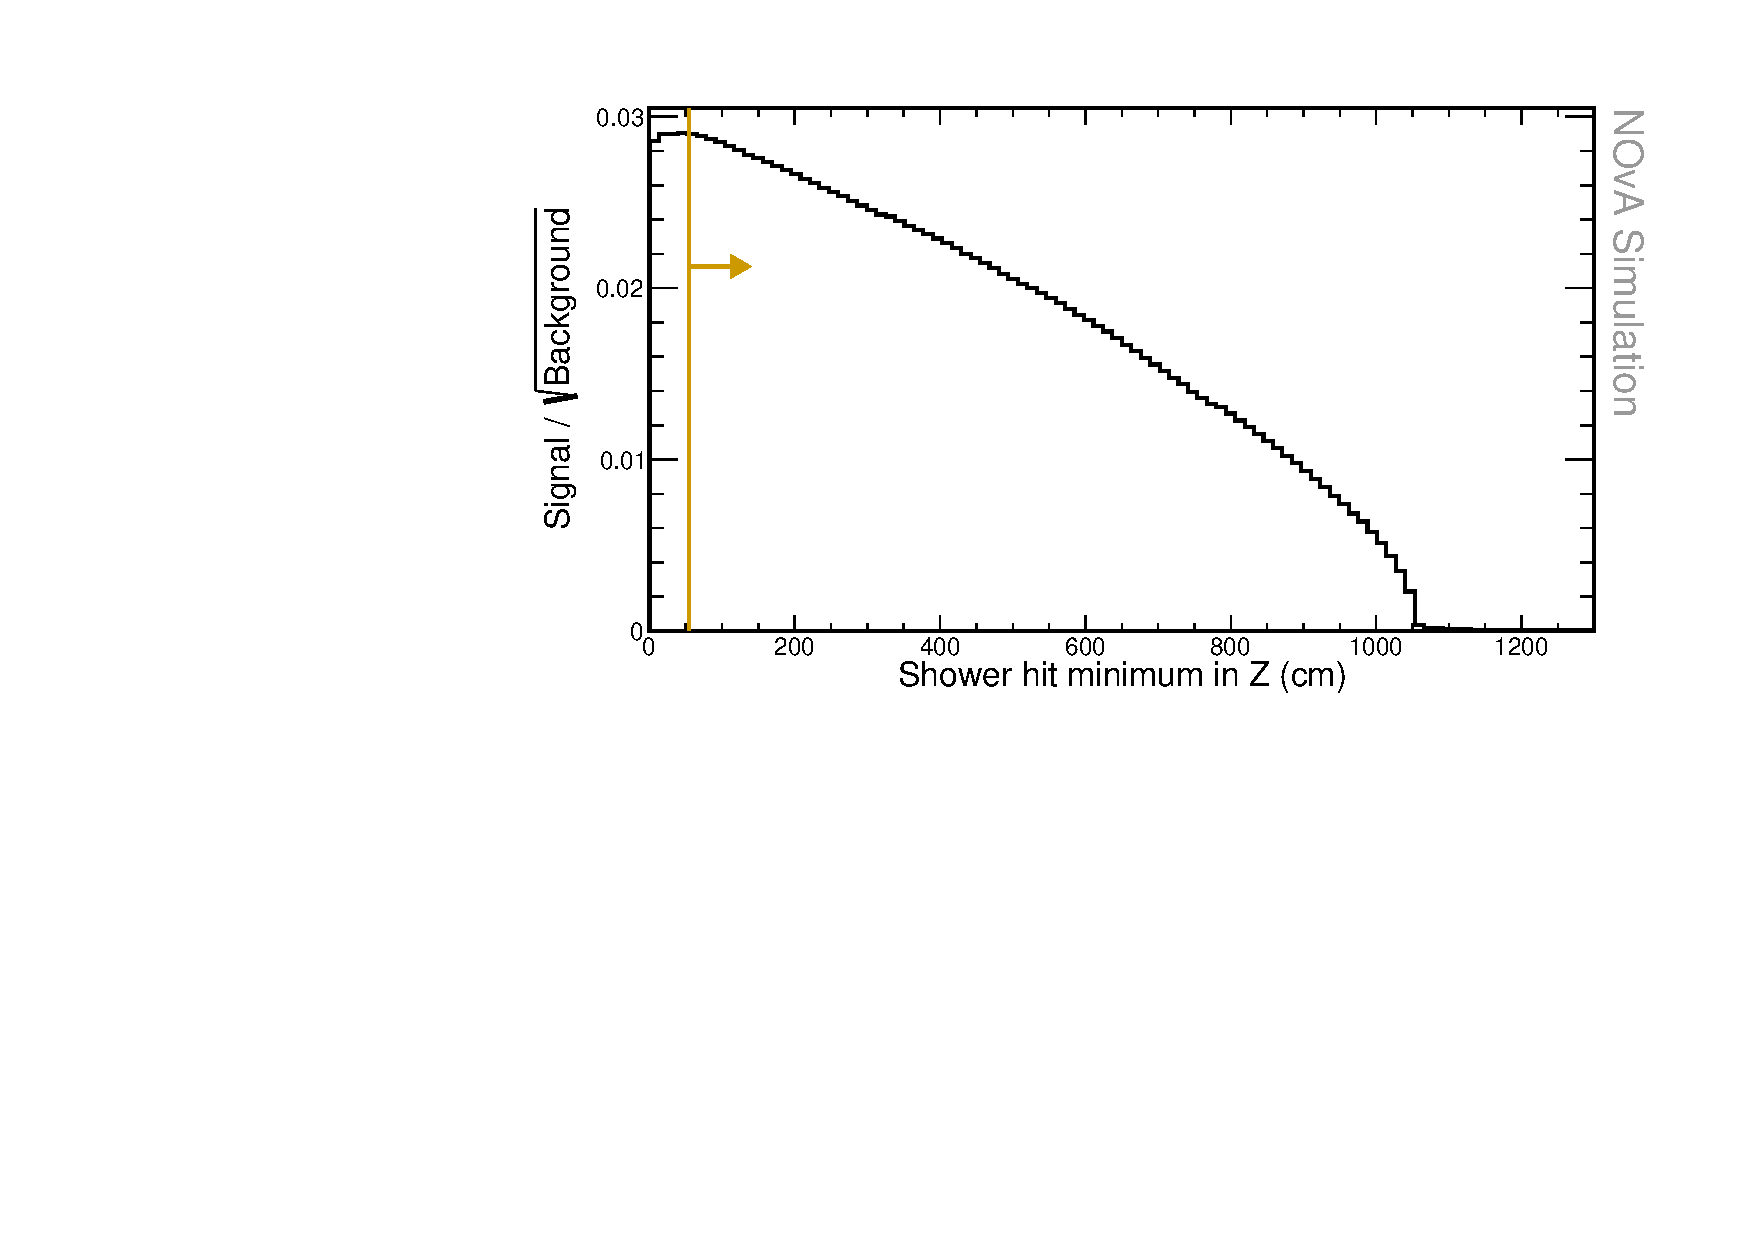
\includegraphics[width=.9\textwidth]{Plots/NuMMEventSelection/NuMM_N1Cut_minZright_FOMStats.pdf}
\caption[Hit minimum z containment cut]{Top: Relative comparison of signal (red), \acrshort{nuone} background (blue), and other background (green) events in the distribution of the minimum hit position of the most energetic prong along the z axis. All histograms are area-normalized. Bottom: Cumulative \acrshort{FOM} calculated as the number of signal events, divided by the number of background events from that bin until the end of the plot in the direction of the yellow arrow. The reconstruction quality, pre-selection and fiducial cuts were applied prior to making these plots. Yellow lines show the cut values that create the containment volume, with arrows pointing towards the preserved events.}
\label{fig:NuMMContainmentCutMinZ}
\end{figure}

\begin{figure}[hbtp]
\centering
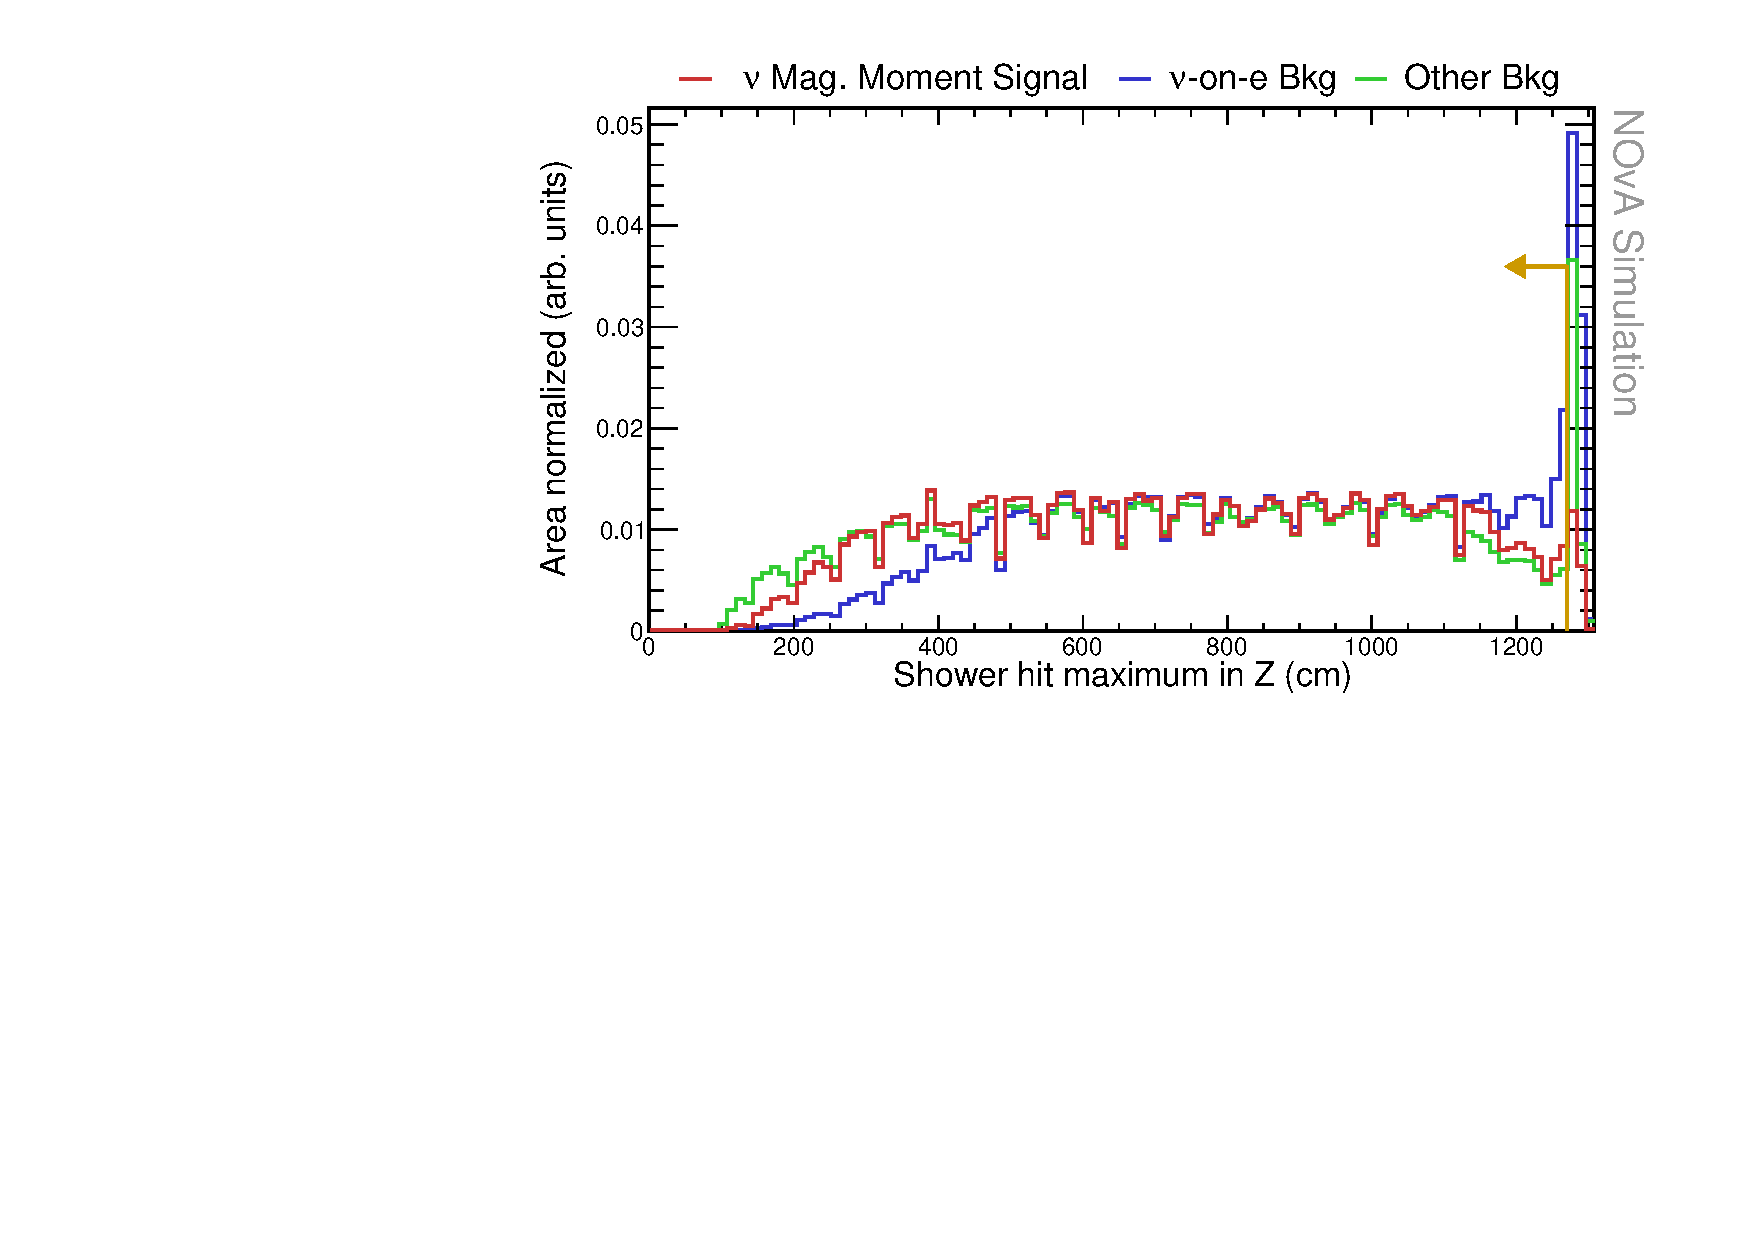
\includegraphics[width=.9\textwidth]{Plots/NuMMEventSelection/N1Cut_maxZ.pdf}
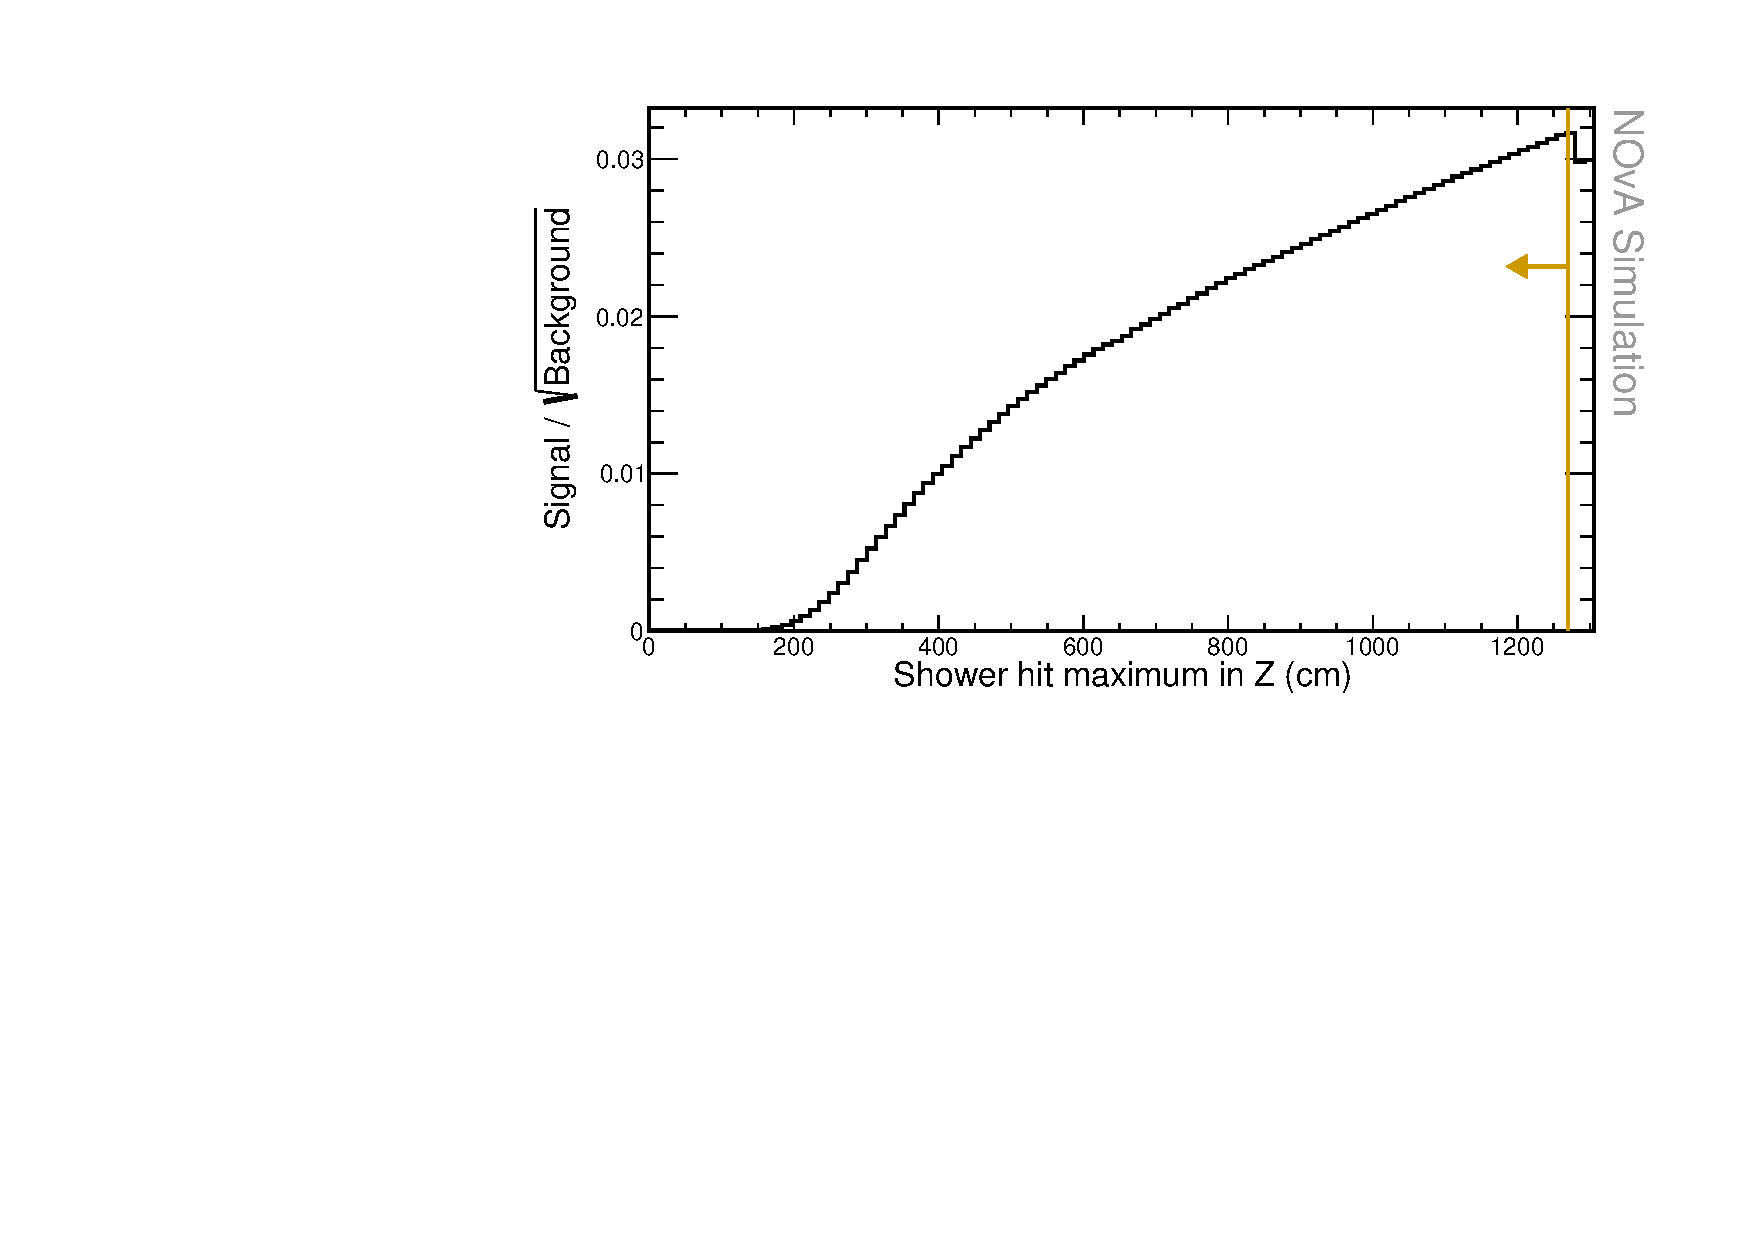
\includegraphics[width=.9\textwidth]{Plots/NuMMEventSelection/NuMM_N1Cut_maxZleft_FOMStats}
\caption[Hit maximum z containment cut]{Top: Relative comparison of signal (red), \acrshort{nuone} background (blue), and other background (green) events in the distribution of the maximum hit position of the most energetic prong along the z axis. All histograms are area-normalized. Bottom: Cumulative \acrshort{FOM} calculated as the number of signal events, divided by the number of background events from that bin until the end of the plot in the direction of the yellow arrow. The reconstruction quality, pre-selection and fiducial cuts were applied prior to making these plots. Yellow lines show the cut values that create the containment volume, with arrows pointing towards the preserved events.}
\label{fig:NuMMContainmentCutMaxZ}
\end{figure}

\begin{table}[!hb]
\centering
\caption[Event selection cutflow table for the containment cuts]{Event selection cutflow table for the containment cuts showing the number of events and the relative efficiency of each cut for each signal sample. The relative efficiency is calculated as number of events remaining after applying the corresponding cut divided by number of event for all the previous cuts. All the cuts are listed in sequence as they are applied. The top row corresponds to the sample after applying the reconstruction quality and pre-selection cuts.}
\begin{tabular}{|l|cc|cc|cc|}\hline
\multicolumn{1}{|c|}{} & \multicolumn{2}{c|}{\textbf{Signal}} & \multicolumn{2}{c|}{\textbf{$\nu$-on-e bkg}} & \multicolumn{2}{c|}{\textbf{Other bkg}} \\
\multicolumn{1}{|c|}{\multirow{-2}{*}{\textbf{Selection}}} & \textbf{$N_{evt}$} & \textbf{$\epsilon_{rel}\left(\%\right)$} & \textbf{$N_{evt}$} & \textbf{$\epsilon_{rel}\left(\%\right)$}  & \textbf{$N_{evt}$} & \textbf{$\epsilon_{rel}\left(\%\right)$}\\\hline
\textbf{Pre-selection} & 155.14 & 100 & 3.33$\times 10^3$ & 100 & 8.83$\times 10^6$ & 100\\
\textbf{Fiducial} & 143.02 & 92.19 & 2.88$\times 10^3$ & 85.60 & 5.96$\times 10^6$ & 67.57\\
\textbf{Containment} & 117.41 & 82.09 & 2.08$\times 10^3$ & 72.12 & 1.10$\times 10^6$ & 18.38\\\hline
\end{tabular}
\label{tab:CutflowTableFiducialContainmnet}
\end{table}

\subsection{Multivariate analysis cuts}\label{sec:NuMMEventSelTMVA}
%%% TMVA
Following the removal of obvious backgrounds and events not contained within the detector, we aim to optimise the event selection to achieve the highest significance for measuring the effective muon neutrino magnetic moment. This goal is equivalent to maximising our \gls{FOM} from Eq.~\ref{eq:NuMMFOM}.

For this purpose, we utilised ROOT's \cite{ROOT} \gls{TMVA} \cite{TMVA}. Specifically, we employed the rectangular cut optimisation method, which uses multivariate parameter fitters to maximise background rejection across the full range of signal efficiencies. We used the \gls{MC} sampling fitting method, assuming that for each input variable, there is a single cut value (maximum or minimum) that optimally discriminates between signal and background.

%Specifically, we are doing this to the inputs, using this number of inputs, these transformations, this algorithms, this distribution of signal and background events with this specific splits, and this number of signal and background events for the evaluation.

%The optimisation of cuts performed by TMVA maximises the background rejection at given signal efficiency, and scans over the full range of the latter quantity. TMVA cut optimisation is performed with the use of multivariate parameter fitters, specifically with the Monte Carlo sampling for us. All optimisation methods (fitters) act on the assumption that one minimum and one maximum requirement on each variable is sufficient to optimally discriminate signal from background (i.e., the signal is clustered). Since I used the fSmart option, my vars are required to have a dedicated min OR max. 

%%%Input variables
\gls{TMVA} generally performs better with a limited number of input variables that have strong discriminating power. Therefore, we investigated several input variables and selected only those that achieved significant background rejection. There are additional variables not mentioned here that might achieve better final results, providing opportunities for future re-analyses. Additionally, we do not apply any transformations to the input variables prior to optimisation, which might also improve the final result after dedicated study.

The variables considered include those already used in the pre-selection: the total number of hits for all prongs in slice, the length of the longest prong, and $E\theta^2$, as discussed in Sec.~\ref{sec:NuMMEventSelectionPresel}. During the \gls{TMVA} optimisation, we found that the length of the longest prong did not significantly enhance discriminating power and thus removed it from the set of input variables. Additionally, we included the reconstructed energy of the most energetic shower, as used for reconstruction quality selection in Sec.~\ref{sec:NuMMEventSelRecoQC}, intending to restrict events with higher energies, since our signal is concentrated at low electron recoil energies.

Additionally, we considered all the variables used for the \gls{NOvA} \gls{nuone} analysis for the neutrino flux constraint \cite{NOVA-doc-56383}. The first is the fraction of the reconstructed energy of the most energetic shower $\left(E_{Shower}\right)$ to the total energy of all the reconstructed prongs in the entire slice $\left(E_{Tot}\right)$. This variable distinguished our signal events, which only have a single shower, from events with multiple showers or additional activity. The second is the gap between the vertex and the most energetic shower, which can distinguish between electron and $\pi^0$ events, as the latter should have a characteristic gap several cells long. Additionally, we examined the amount of energy contained within $\pm8$ planes away from the vertex, besides the energy associated with the most energetic prong, which should distinguish the purely leptonic signal from backgrounds with significant hadronic activity. However, the gap and the vertex energy variables underperformed compared to others and were ultimately not used within the \gls{TMVA}.

We also utilised two \gls{CNN}-based event classifiers developed for the \gls{NOvA} \gls{nuone} analysis for the neutrino flux constraint \cite{NOVA-doc-56383, Nuone_Neutrino2022Poster}. These classifiers are specifically designed to identify \gls{nuone} interactions. The first, named \acrshort{nuoneID}, is trained to select \gls{nuone} events from the primary $\nu_\mu$\gls{CC} background, while the second, named \acrshort{EPi0ID}, is trained on events passing the \acrshort{nuoneID} selection to reject the remaining background with a $\pi^0$. These classifiers use a pixel map of the entire slice as input and are designed with the same \gls{CNN} architecture as ProngCVN and EventCVN described in Sec.~\ref{sec:NOvAReconstruction}.

%[ND group's technote] Two event classifiers (NuoneID and Epi0ID) based on convolutional neural network (CNN) are trained to identify nuone elastic scattering events (NuoneID) and to further reject background with pi0 in the final state (Epi0ID). The CNN architecture adopted for this analysis is the one used for NOvA CVN [12]. It takes the pixel map of a slice as the input and has deeper and more complicated neural networks than the ANNs used in the previous round of analysis [11]. The training for both classifiers (NuoneID and Epi0ID) were done with single electron samples as the signal in order to mitigate the model dependence. A nuone elastic scattering has an electron in the final state which could deposit energy in the detector. Single electron events share this feature with nuone elastic scattering, but have more uniform distribution of energy, angle between the shower direction and the beam direction. This additional feature could prevent CNN models from overfitting the feature of the very small scattering angle.  To make comparisons, test samples of signal and background are normalized to 1.1E21. The output categories are \gls{nuone}, $\pi^0$, $\nu_e$\gls{CC} and other. The \gls{nuone} and $\pi^0$ outputs are used for the training of the Epi0ID. The pre-selection applied is: ND group's preselection ($L<\unit[800]{cm}$, $N_{plane}<120$, $N_{cell}<600$), loose containment ($-190<X<190$, $-190<Y<190$, $50<Z<1500$ $\unit{cm}$), loose single particle cut ($E_{vtx}<\unit[0.05]{GeV}$, $gap<\unit[20]{cm}$, $E_{shower}/E_{tot} > 0.9$ \note{These are quite strict actually}. The training accuracy for NuoneID is about 85\% and for Epi0ID is about 96\%. After each round of training, the trained model is saved to make predictions on the test sample so we know how the actual performance of the classifiers evolves over different epochs.

%%% Result
The result of the \gls{TMVA} is a set of cuts on each of the input variables that maximises the \gls{FOM}. The input variables and the cuts that were selected for them are shown in Fig.~\ref{fig:NuMMCutsTMVA1}, \ref{fig:NuMMCutsTMVA2}, and \ref{fig:NuMMCutsTMVA3}. The effect of these cuts is summarised in Tab.~\ref{tab:CutflowTableTMVA}. Applying the \gls{TMVA} cuts reduces the signal by $\unit[51.62]{\%}$, the \gls{nuone} background by $\unit[75.03]{\%}$ and other background by $\unit[99.98]{\%}$. The specific values of the cuts resulting from the \gls{TMVA} are
\begin{align}
E_{Shower}/E_{Tot} &> 0.91,\\
\textsf{Total N}^o\textsf{ hits for all prongs} &< 116,\\
E_{Shower} &< \unit[1.4]{GeV},\\
E\theta^2 &< \unit[0.0048]{GeV\times rad^2},\\
\acrshort{nuoneID} &> 0.65,\\
\acrshort{EPi0ID} &> 0.63.
\end{align}

\begin{figure}[hbtp]
\centering
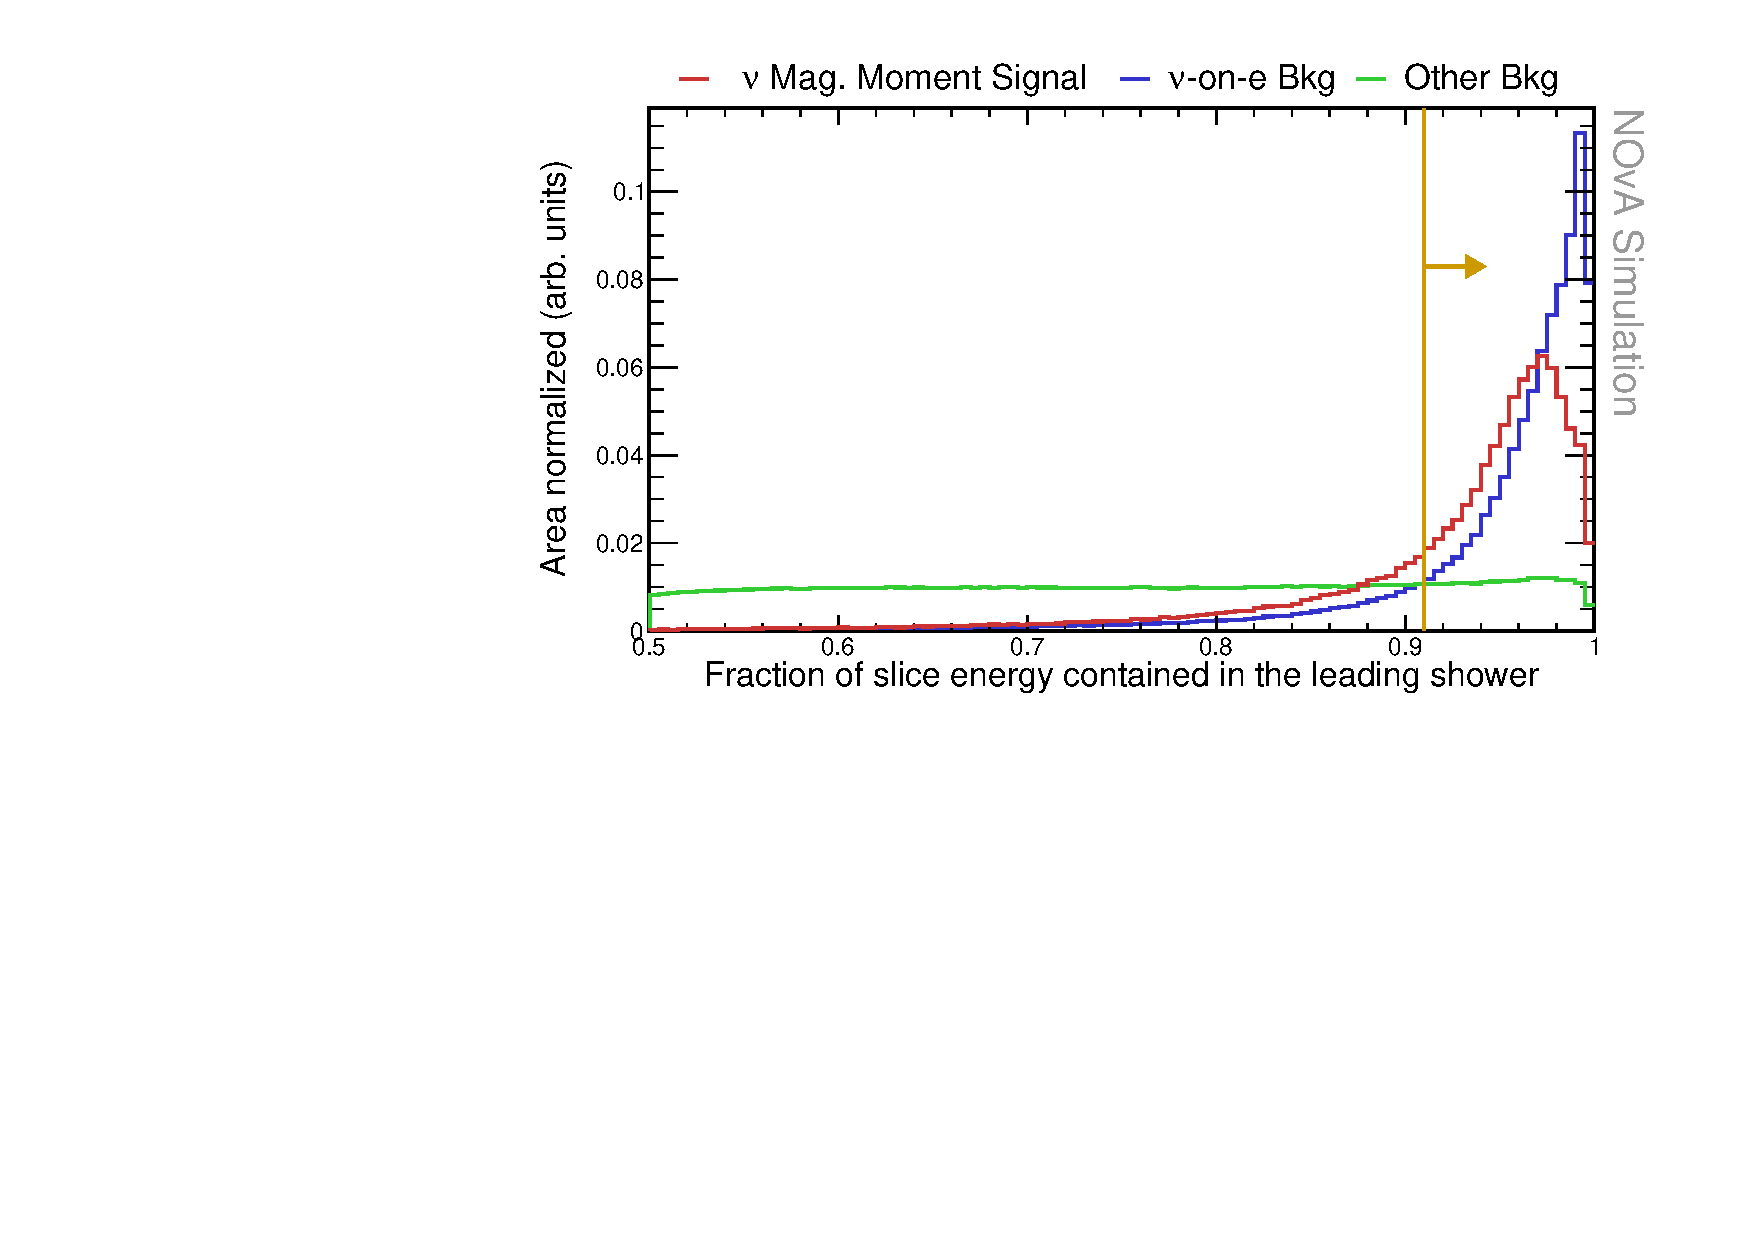
\includegraphics[width=.9\textwidth]{Plots/NuMMEventSelection/N1Cut_shwEFrac.pdf}
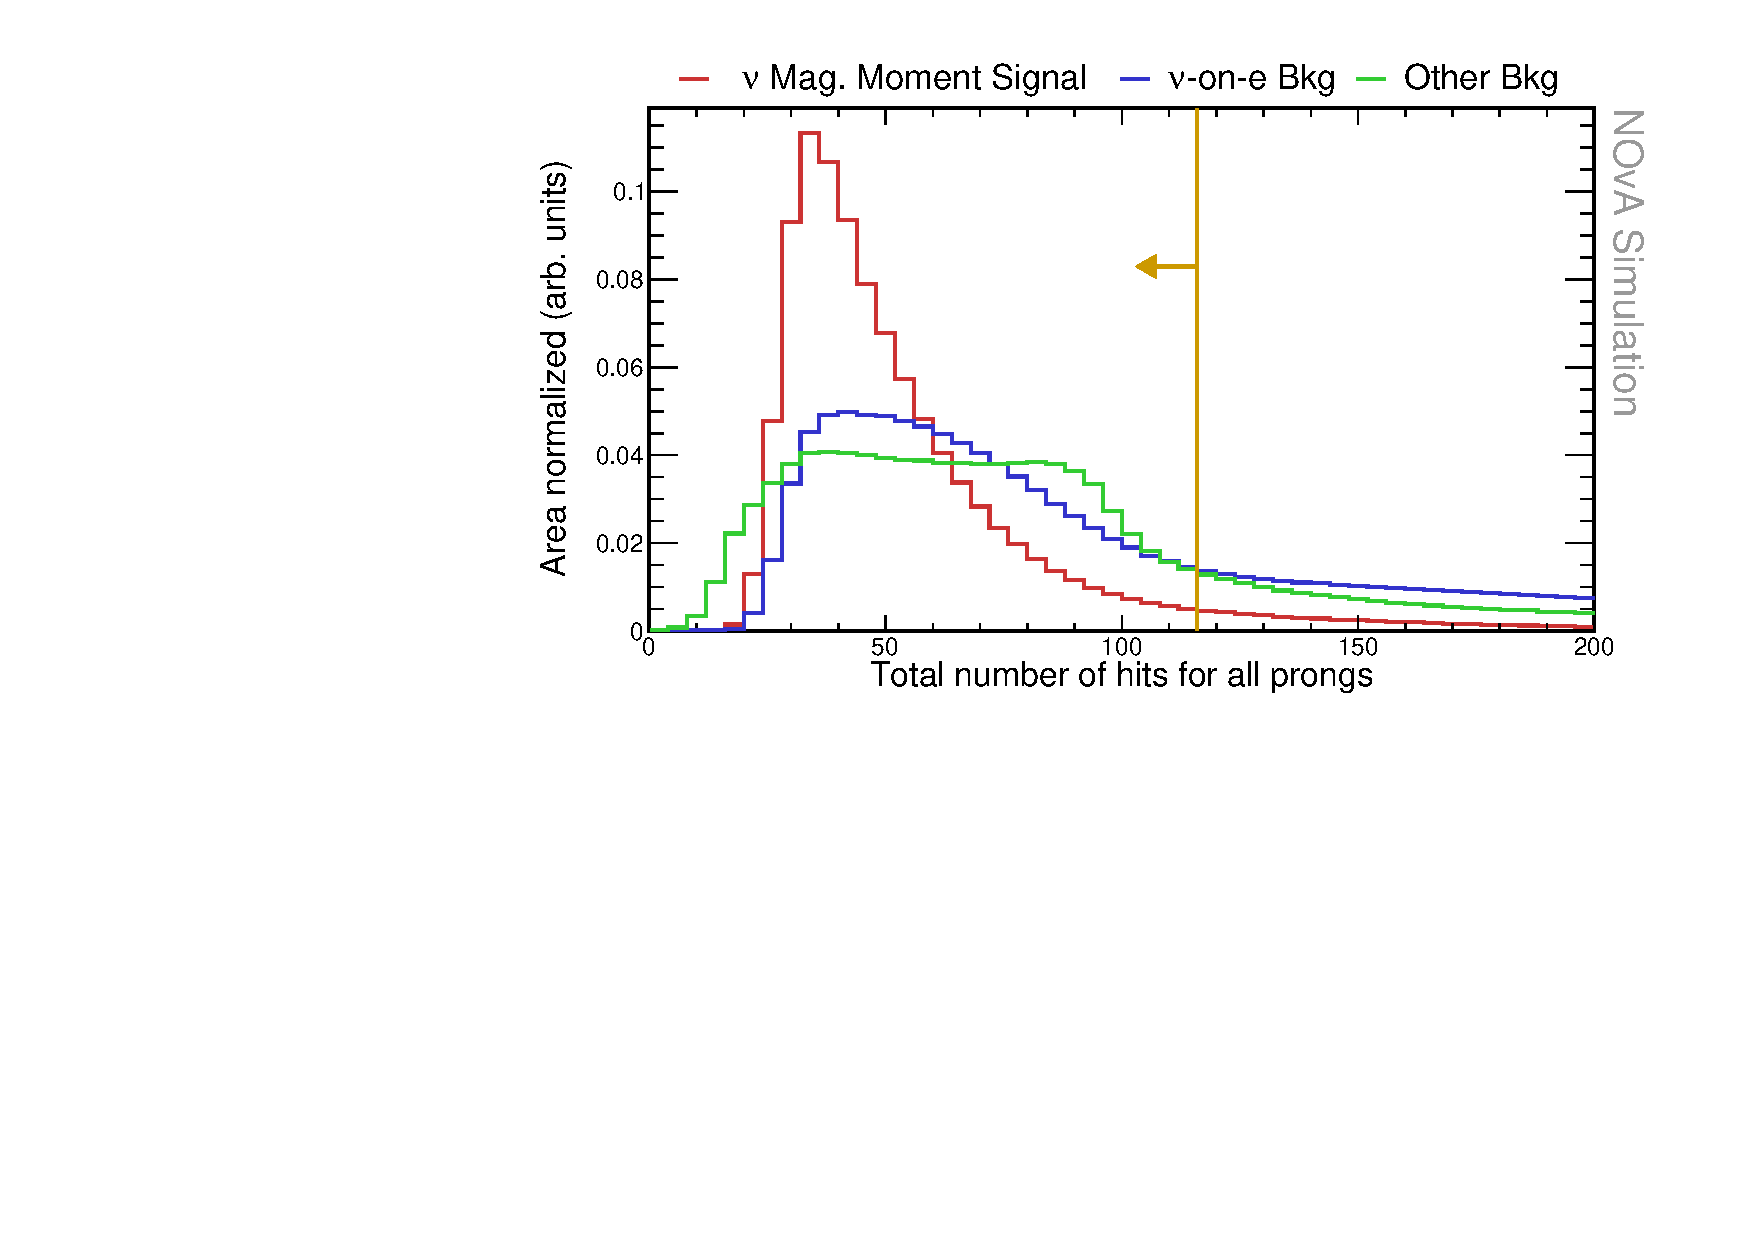
\includegraphics[width=.9\textwidth]{Plots/NuMMEventSelection/N1Cut_NHitsPre.pdf}
\caption[Shower E fraction and number of hits cuts]{Relative comparison of signal (red), \acrshort{nuone} background (blue), and other background (green) events in the distribution of the fraction of the total energy contained in the primary shower (top) and of the total number of hits in the slice (bottom). All histograms are area-normalized. The reconstruction quality, pre-selection, fiducial and containment cuts were applied prior to making these plots. Yellow lines show the cut values on the depicted variables, with arrows pointing towards the preserved events.}
\label{fig:NuMMCutsTMVA1}
\end{figure}

\begin{figure}[hbtp]
\centering
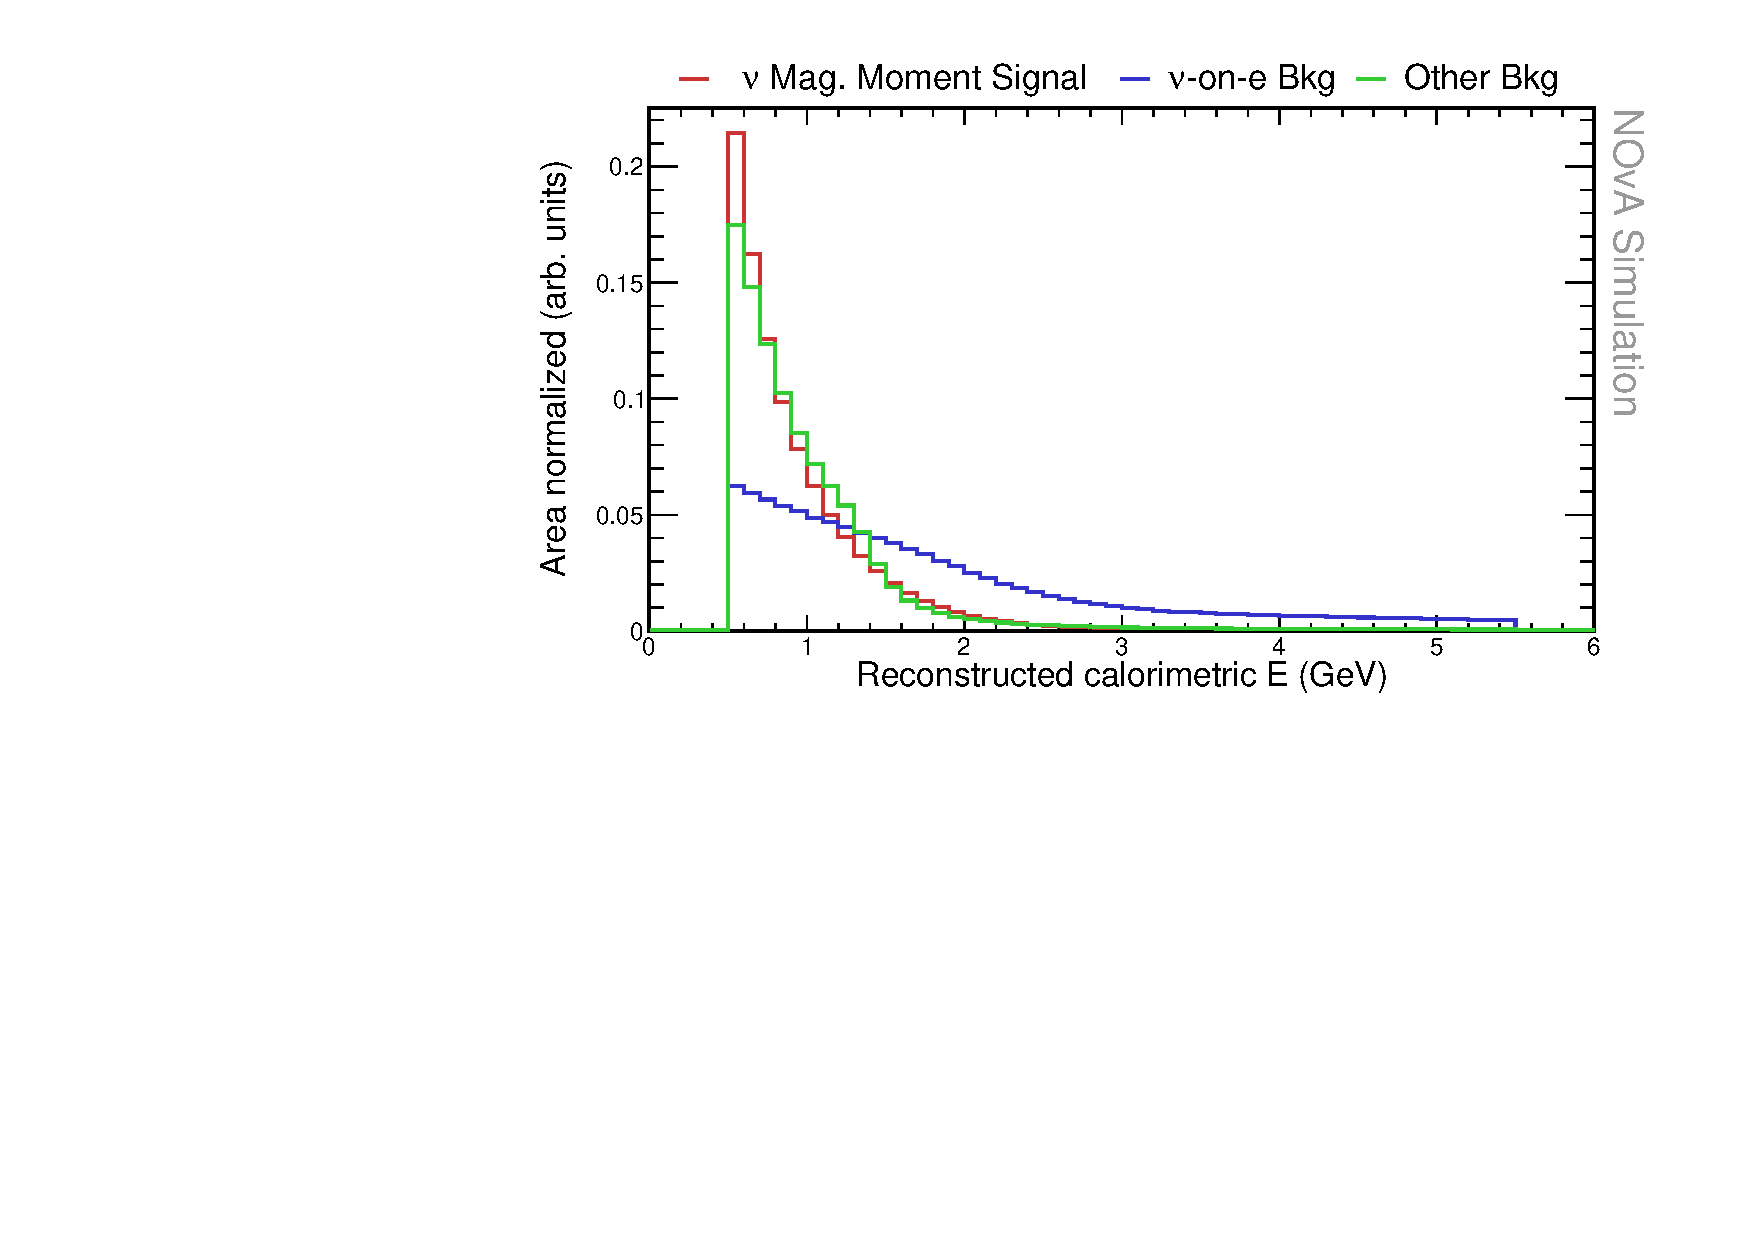
\includegraphics[width=.9\textwidth]{Plots/NuMMEventSelection/N1Cut_calEHighPre.pdf}
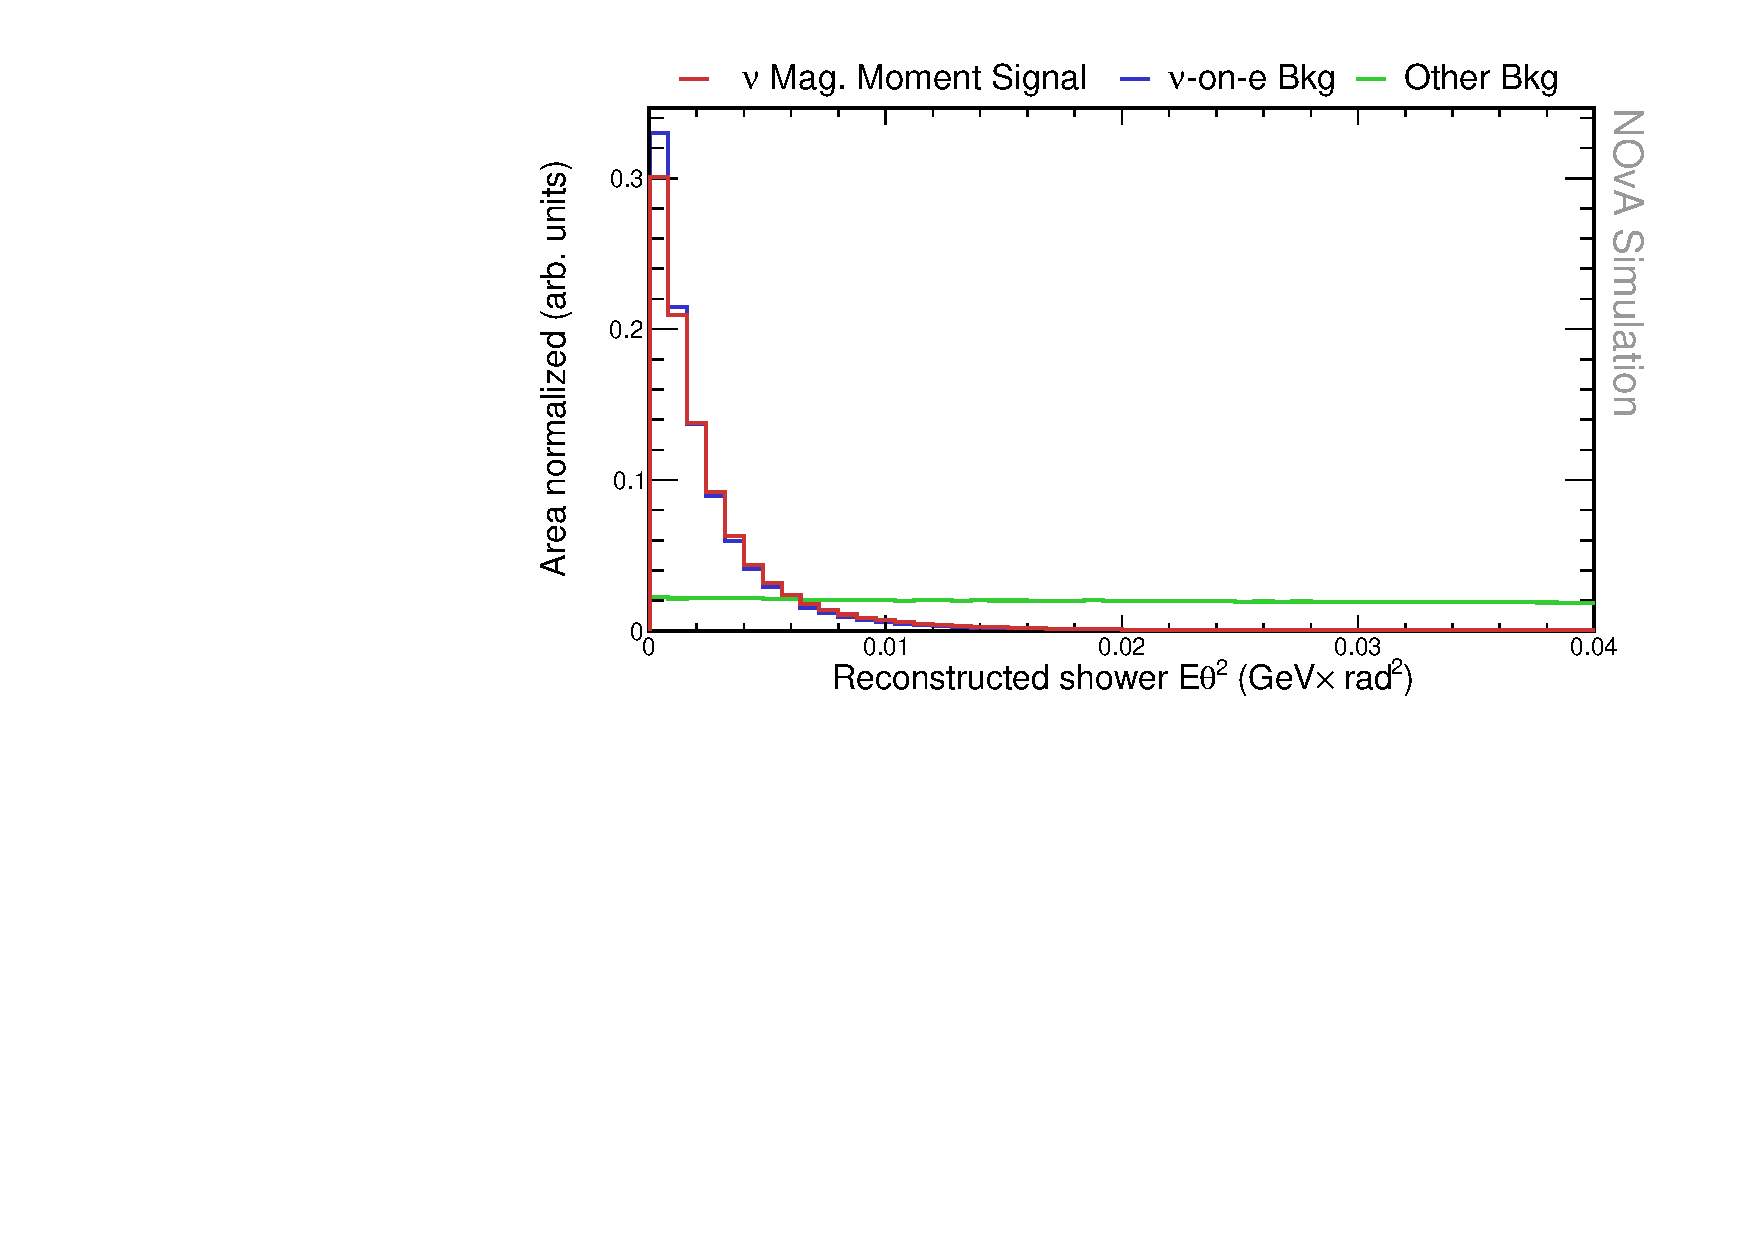
\includegraphics[width=.9\textwidth]{Plots/NuMMEventSelection/N1Cut_eth2Pre.pdf}
\caption[Reconstructed energy and $E\theta^2$ cuts]{Relative comparison of signal (red), \acrshort{nuone} background (blue), and other background (green) events in the distribution of the reconstructed energy of the primary shower (top) and of the reconstructed energy multiplied by the angle from the incoming neutrino beam direction squared (bottom). All histograms are area-normalized. The reconstruction quality, pre-selection, fiducial and containment cuts were applied prior to making these plots. Yellow lines show the cut values on the depicted variables, with arrows pointing towards the preserved events.}
\label{fig:NuMMCutsTMVA2}
\end{figure}

\begin{figure}[hbtp]
\centering
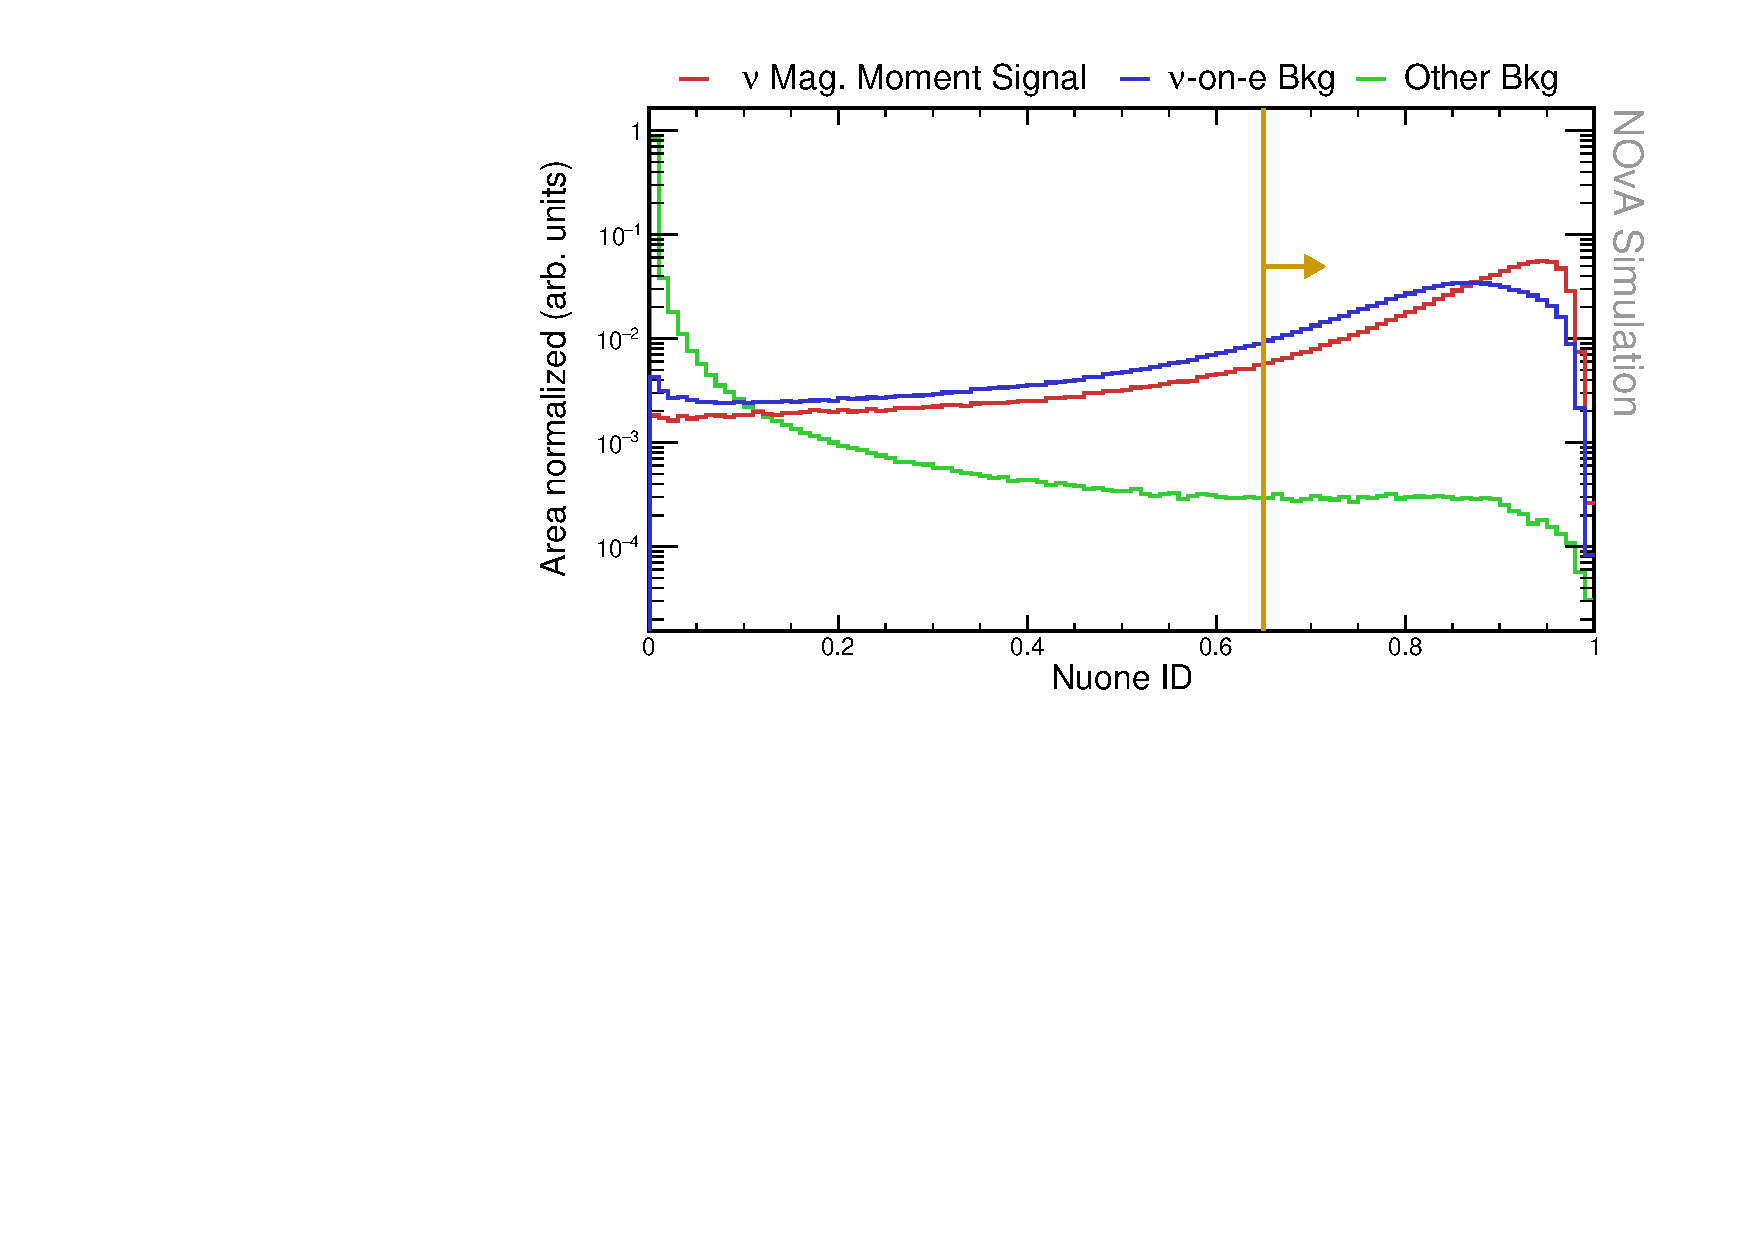
\includegraphics[width=.9\textwidth]{Plots/NuMMEventSelection/LogY_N1Cut_nuoneidPre.pdf}
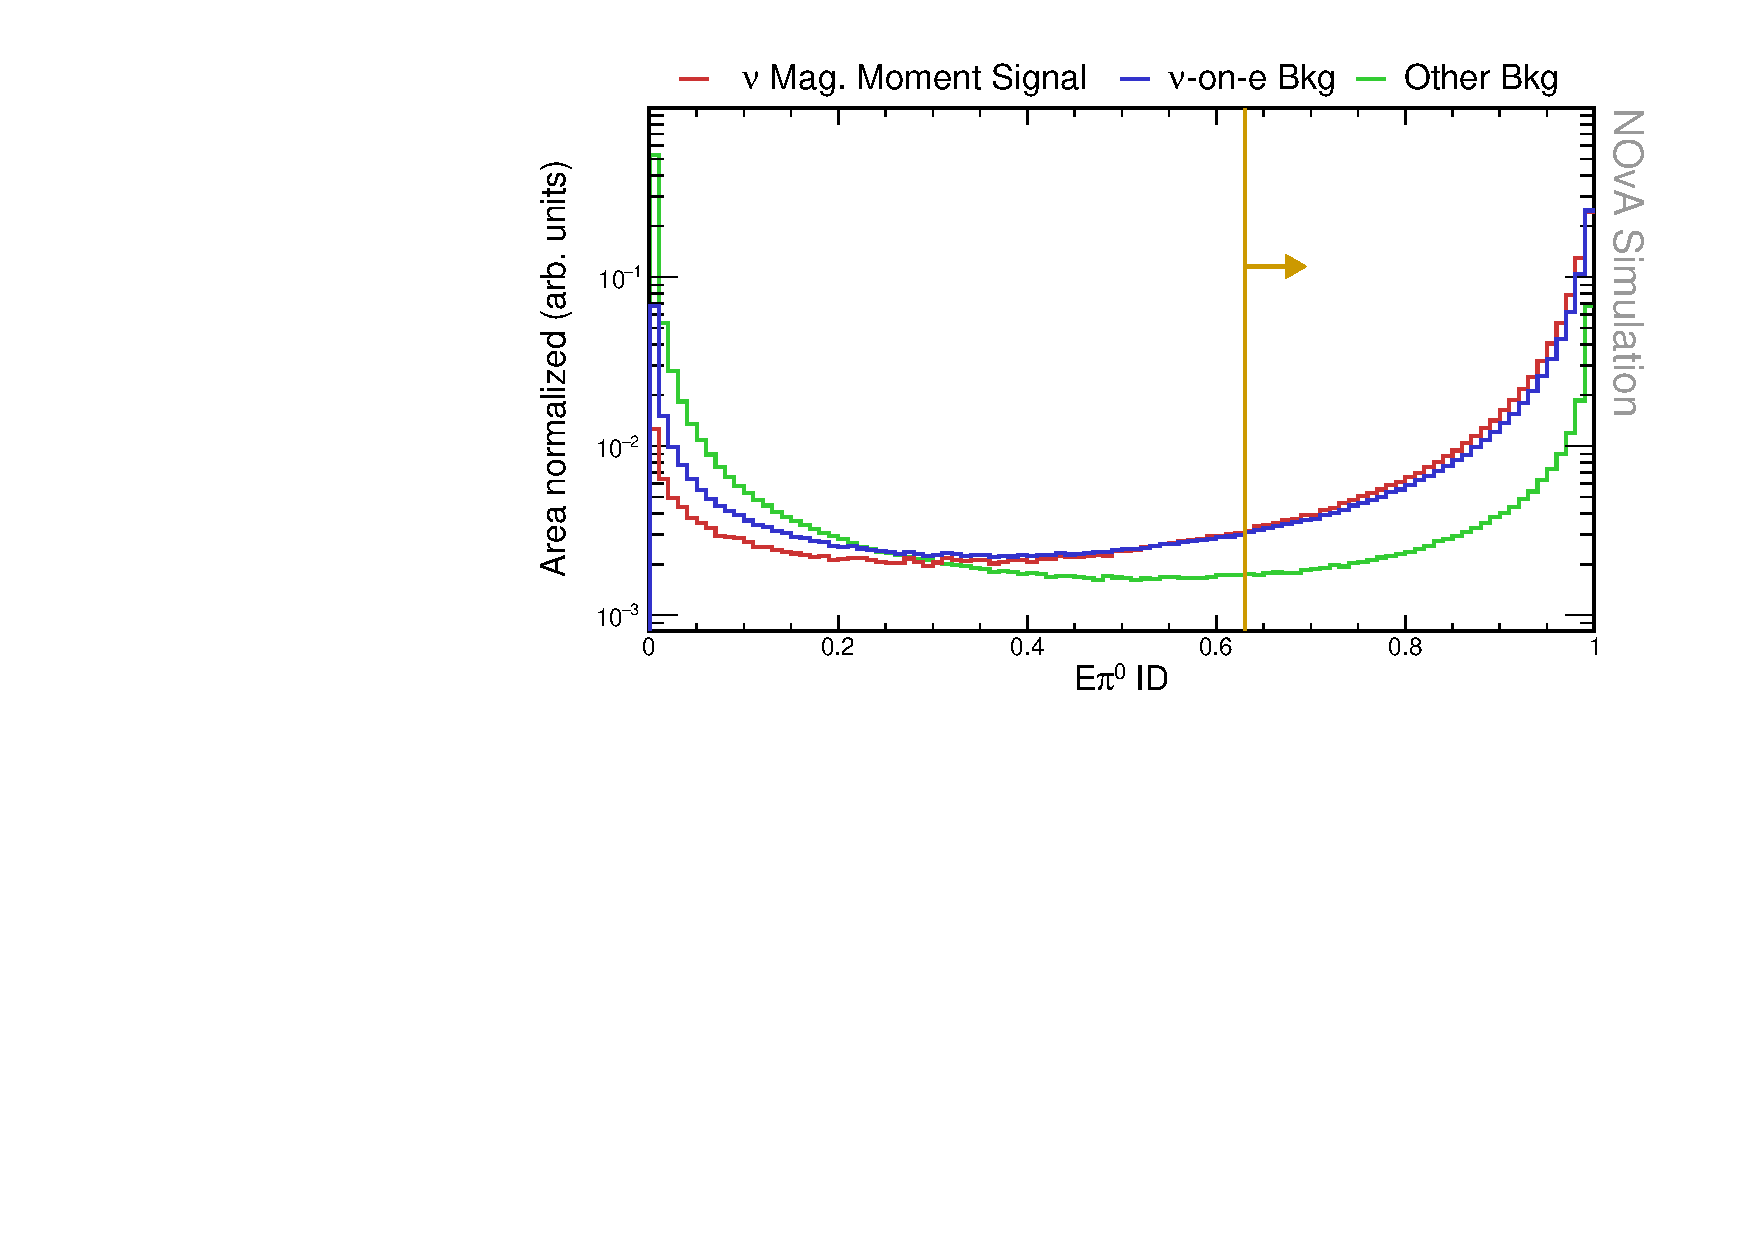
\includegraphics[width=.9\textwidth]{Plots/NuMMEventSelection/LogY_N1Cut_epi0idPre.pdf}
\caption[NuoneID and EPi0ID cuts]{Relative comparison of signal (red), \acrshort{nuone} background (blue), and other background (green) events in the distribution of the \acrshort{nuoneID} (top) and \acrshort{EPi0ID} (bottom) event identifiers. All histograms are area-normalized and logarithmic in the y axis. The reconstruction quality, pre-selection, fiducial and containment cuts were applied prior to making these plots. Yellow lines show the cut values on the depicted variables, with arrows pointing towards the preserved events.}
\label{fig:NuMMCutsTMVA3}
\end{figure}

\begin{table}[!hb]
\centering
\caption[Multivariate analysis cutflow table]{Event selection cutflow table for the results of the cut-based Multivariate analysis, showing the number of events and the relative efficiency of each cut for each signal sample. The relative efficiency is calculated as number of events remaining after applying the corresponding cut divided by number of event for all the previous cuts. All the cuts are listed in sequence as they are applied. The top row corresponds to the sample after applying the reconstruction quality, pre-selection, fiducial and containment cuts.}
\begin{tabular}{|l|cc|cc|cc|}\hline
\multicolumn{1}{|c|}{} & \multicolumn{2}{c|}{\textbf{Signal}} & \multicolumn{2}{c|}{\textbf{$\nu$-on-e bkg}} & \multicolumn{2}{c|}{\textbf{Other bkg}} \\
\multicolumn{1}{|c|}{\multirow{-2}{*}{\textbf{Selection}}} & \textbf{$N_{evt}$} & \textbf{$\epsilon_{rel}\left(\%\right)$} & \textbf{$N_{evt}$} & \textbf{$\epsilon_{rel}\left(\%\right)$}  & \textbf{$N_{evt}$} & \textbf{$\epsilon_{rel}\left(\%\right)$}\\\hline
\textbf{Contained} & 117.41 & 100 & 2.08$\times 10^3$ & 100 & 1.10$\times 10^6$ & 100\\
\textbf{$E_{Shower}/E_{Tot}$} & 113.03 & 96.28 & 2.02$\times 10^3$ & 97.32 & 4.53$\times 10^5$ & 41.30\\
\textbf{N$^o$ Hits} & 106.48 & 94.20 & 1.45$\times 10^3$ & 71.53 & 4.02$\times 10^5$ & 88.78\\
\textbf{High $E_{Shower}$} & 85.51 & 80.31 & 777.91 & 53.76 & 3.01$\times 10^5$ & 74.84\\
\textbf{\acrshort{nuoneID}} & 72.23 & 84.47 & 652.32 & 83.86 & 4.40$\times 10^3$ & 1.46\\
\textbf{\acrshort{EPi0ID}} & 67.35 & 93.24 & 608.19 & 93.23 & 2.83$\times 10^3$ & 64.34\\
\textbf{$E\theta^2$} & 56.80 & 84.33 & 519.09 & 85.35 & 181.24 & 6.40\\\hline
\end{tabular}
\label{tab:CutflowTableTMVA}
\end{table}

After the full event selection, the predicted number of signal events for $\mu_\nu~=~10^{-9}\mu_B$ is $56.80$, and the total number of background events under the \gls{SM} hypothesis is $700.33$. The decomposition of background into interaction types is shown in Fig.~\ref{fig:NuMMBackgroundDecomposition} and listed in Tab.~\ref{tab:NuMMBackgroundContributions}. The event selection results in
\begin{equation}
\textsf{Signal Purity}=\frac{\textsf{Signal}}{\textsf{Signal+Background}}=\unit[7.50]{\%},
\end{equation}
\begin{equation}
\textsf{Signal Efficiency}=\frac{\textsf{Signal}}{\textsf{Signal}_{\textsf{No Cut}}}=\unit[6.95]{\%}.
\end{equation}
Also,
\begin{equation}
\frac{\textsf{Signal}}{\sqrt{\textsf{Background}}}=2.15
\end{equation}
and
\begin{equation}
\textsf{\gls{FOM}}=\frac{\textsf{Signal}}{\sqrt{\textsf{Signal+Background}}}=2.06.
\end{equation}

\begin{table}[!hb]
\centering
\caption[Interactions contributing to the SM background]{Interaction types contributing to the \acrshort{SM} background after full event selection. Interactions with/without $\pi^0$ in the final state are specifically selected due to their significant contribution to the \acrshort{nuone} background.}
\begin{tabularx}{.5\textwidth}{@{}X@{}}
\textbf{Interaction} \hfill \textbf{Number of events}\\\hline
\gls{nuone} \dotfill 519.09\\
\gls{NC} w/$\pi^0$ \dotfill 72.96\\
\gls{NC} w/o $\pi^0$ \dotfill 21.51\\
$\nu_\mu$\gls{CC} w/$\pi^0$ \dotfill 28.07\\
$\nu_\mu$\gls{CC} w/o $\pi^0$ \dotfill 25.67\\
$\nu_e$\gls{CC}\gls{MEC} \dotfill 2.22\\
Other $\nu_e$\gls{CC} \dotfill 9.83\\
Other \dotfill 20.98\\\hline
\textbf{Total} \dotfill 700.33\\
\end{tabularx}
\label{tab:NuMMBackgroundContributions}
\end{table}

\begin{figure}[hbtp]
\centering
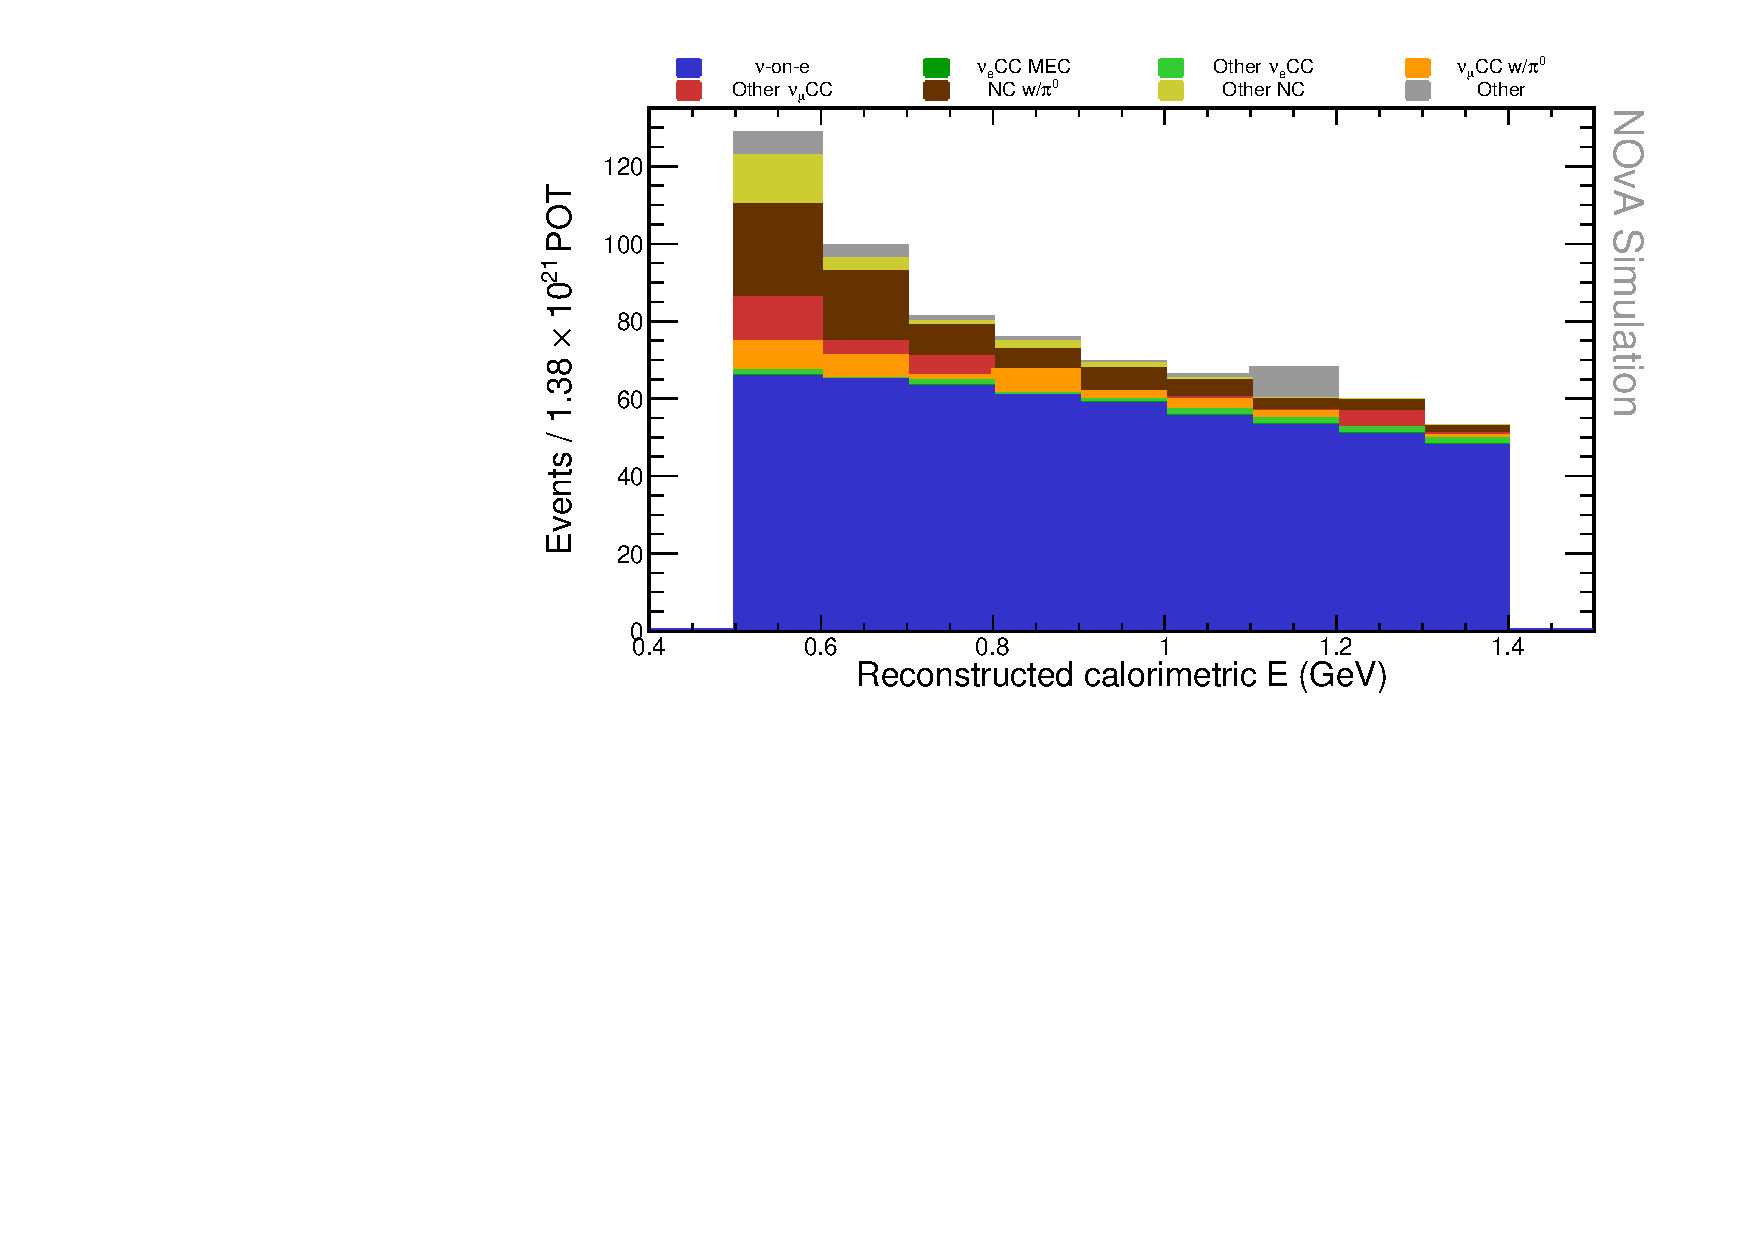
\includegraphics[width=\textwidth]{Plots/NuMMEventSelection/N1Cut_calESignal.pdf}
\caption[Background composition of final selection]{Background composition of events passing the full event selection as a function of the reconstructed energy of the leading shower - electron for \acrshort{nuone} events. Events are scaled to the data exposure. Origin of the `Other' background events between $\unit[1.1-1.2]{GeV}$ is not known.}
\label{fig:NuMMBackgroundDecomposition}
\end{figure}

%There are possible improvements in trying different \gls{MVA} methods, namely \gls{BDT} and so on. Since we are using the standard \gls{NOvA} simulation sample, implementation of new event identifiers into the workflow would be very complicated, unless done when updating the production. 

%%%%%%%%%%%%%%%%%%%%%%%%%%%%%%%%%%%%%%%%%%%%%%%%%%%%%%%%%%%%%%%%%%%%%
%%%                   RESOLUTION AND BINNING                      %%%
%%%%%%%%%%%%%%%%%%%%%%%%%%%%%%%%%%%%%%%%%%%%%%%%%%%%%%%%%%%%%%%%%%%%%
\iffalse
\section{Energy resolution and binning}\label{sec:NuMMResolution}
\todo{Add the energy resolution and binning plots}
Describe what events were used for the energy resolution study and how it was performed

What are the results

Final plot

The electron energy and angle distributions and resolutions. Are we going to fit in E, Th, or ETh2? Is there something else?

Show plots of Reco V True for both energy and angle. (Should I show it with or without the energy cut?). Also show the resolution plots.

Maybe also mention that Test Beam will help with improving the dead materials correction and generally improving the bias and resolution of the reconstructed energy, which won't have to depend on the comparison to simulation
\fi
%%%%%%%%%%%%%%%%%%%%%%%%%%%%%%%%%%%%%%%%%%%%%%%%%%%%%%%%%%%%%%%%%%%%%
%%%                    SYSTEMATIC UNCERTAINTIES                   %%%
%%%%%%%%%%%%%%%%%%%%%%%%%%%%%%%%%%%%%%%%%%%%%%%%%%%%%%%%%%%%%%%%%%%%%
\section{Systematic uncertainties}\label{sec:NuMMSystematics}

We consider all the standard \gls{NOvA} systematic uncertainties described in Sec.~\ref{sec:NOvASystematics}, grouped into four categories: neutrino flux, detector calibration, detector modelling, and neutrino interaction systematic uncertainties. Summary of the effects of both systematic and statistical uncertainties on the predicted number of \gls{SM} background events is shown in Fig.~\ref{fig:NuMMErrorBarChart}. The four categories of systematic uncertainties are assumed to be uncorrelated between each other, allowing to calculate their combined effect by adding their individual contribution in quadrature. The statistical uncertainty is calculated as $\sqrt{N_{\gls{SM}}}$ since the number of predicted events follows the Poisson distribution. The total prediction of the number of \gls{SM} background events can be expressed as
\begin{equation}\label{eq:NumberOfSMEventsWithSysts}
N_{\gls{SM}}=700.33 \pm 26.46\left(\textsf{stat.}\right) ^{+72.48}_{-62.99}\left(\textsf{syst.}\right).
\end{equation}

\begin{figure}[hbtp]
\centering
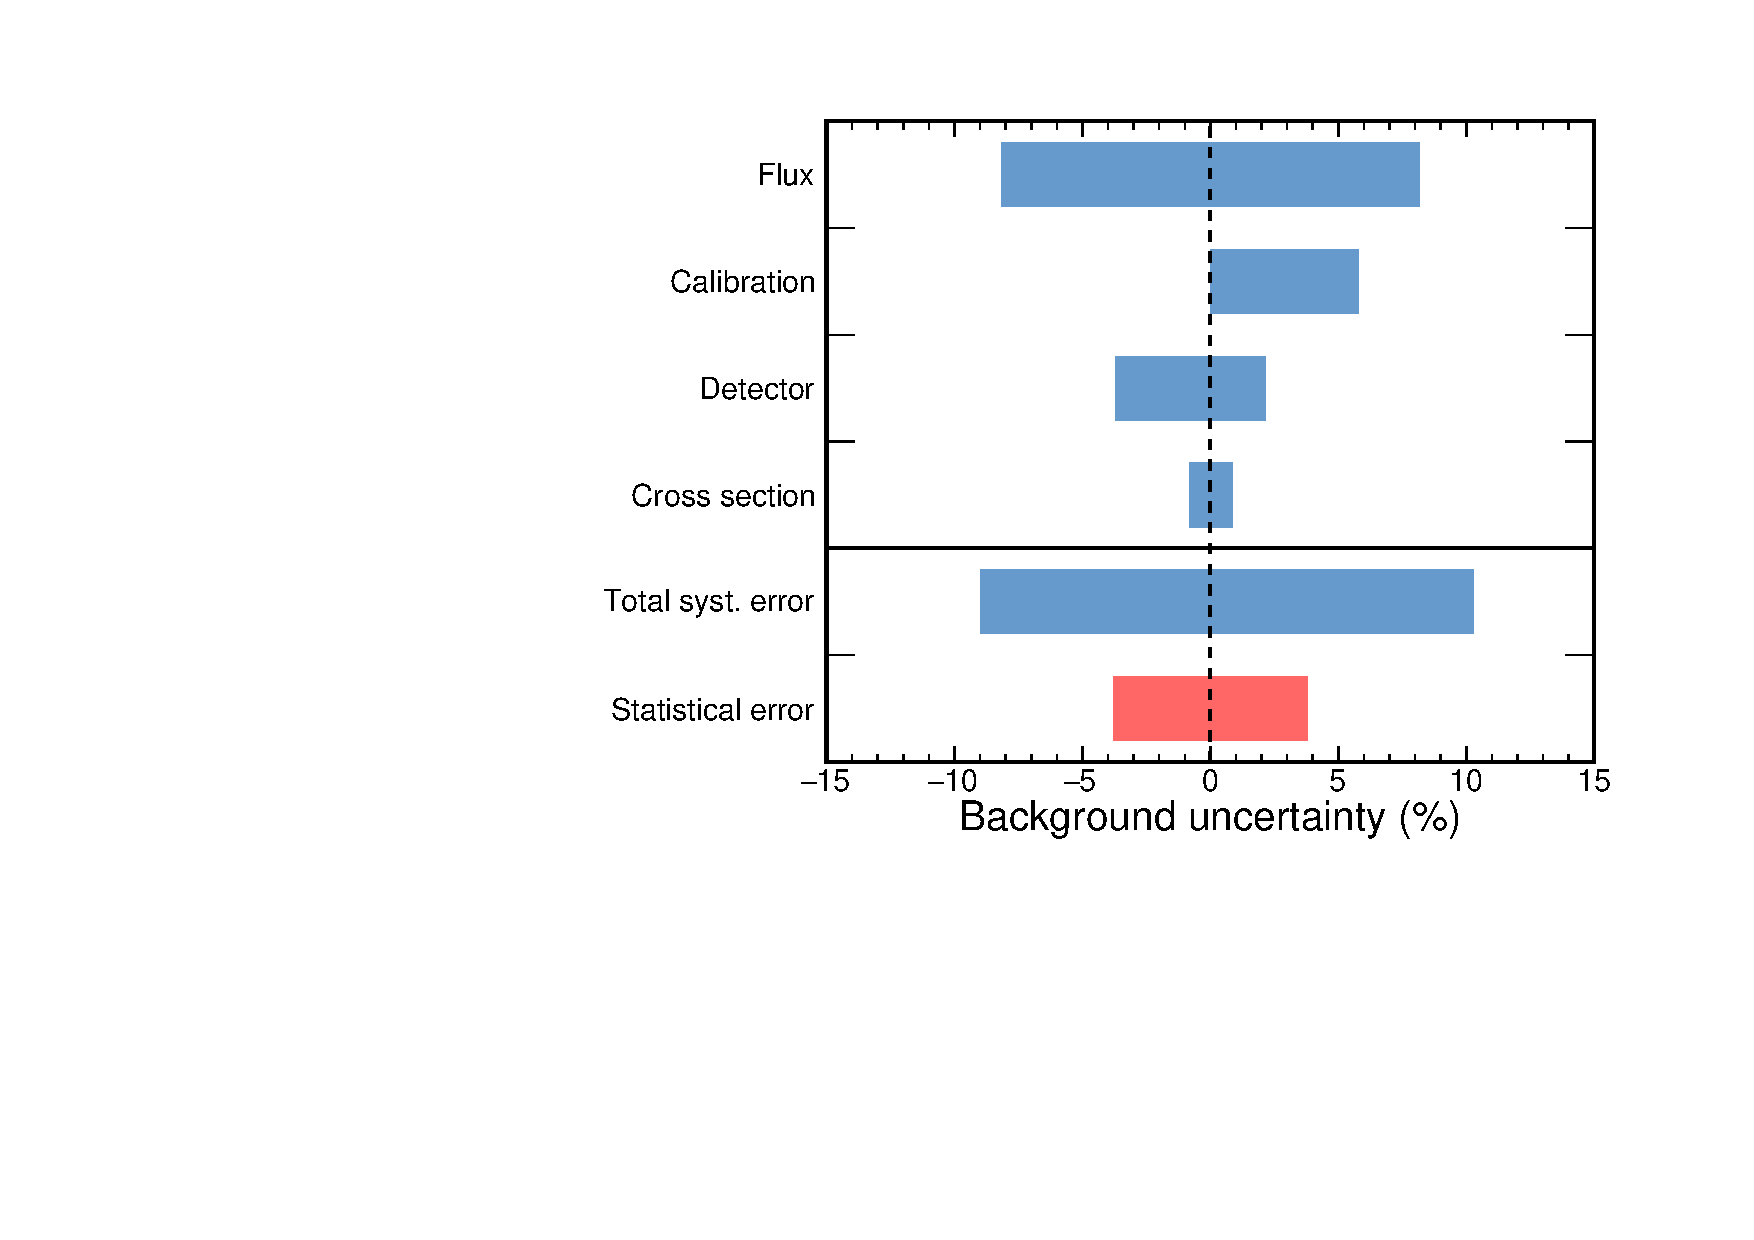
\includegraphics[width=.9\textwidth]{Plots/NuMM/RelativeErrorBarChart.pdf}
\caption[Summary of systematic uncertainties]{Relative effect of systematic and statistical uncertainties on the number of \acrshort{SM} background events. The total systematic uncertainty (blue bottom bar) is calculated as a square root of the sum of squares of the four categories of systematic uncertainties, shown ordered by the size of their effect. These are the neutrino flux, detector calibration, detector modelling, and neutrino cross section systematic uncertainties.}
\label{fig:NuMMErrorBarChart}
\end{figure}

To assess the effect of the neutrino flux systematic uncertainty, we use 8 \gls{ND}-only principal components. Figure~\ref{fig:NuMMFluxSysts} shows their combined effect on the predicted \gls{SM} background as a function of the primary shower's reconstructed energy. Since the principal components are uncorrelated by construction, the total systematic uncertainty for each bin is calculated by adding the effect of all the principal components in quadrature. The effect of the neutrino flux systematic uncertainty does not depend on the primary shower's calorimetric energy and altering the neutrino flux prediction can be represented by a normalization shift. The final effect of the neutrino flux systematic uncertainty on the total number of \gls{SM} background events is $\pm\unit[8.16]{\%}$ and is symmetric around the nominal prediction.

\begin{figure}[hbtp]
\centering
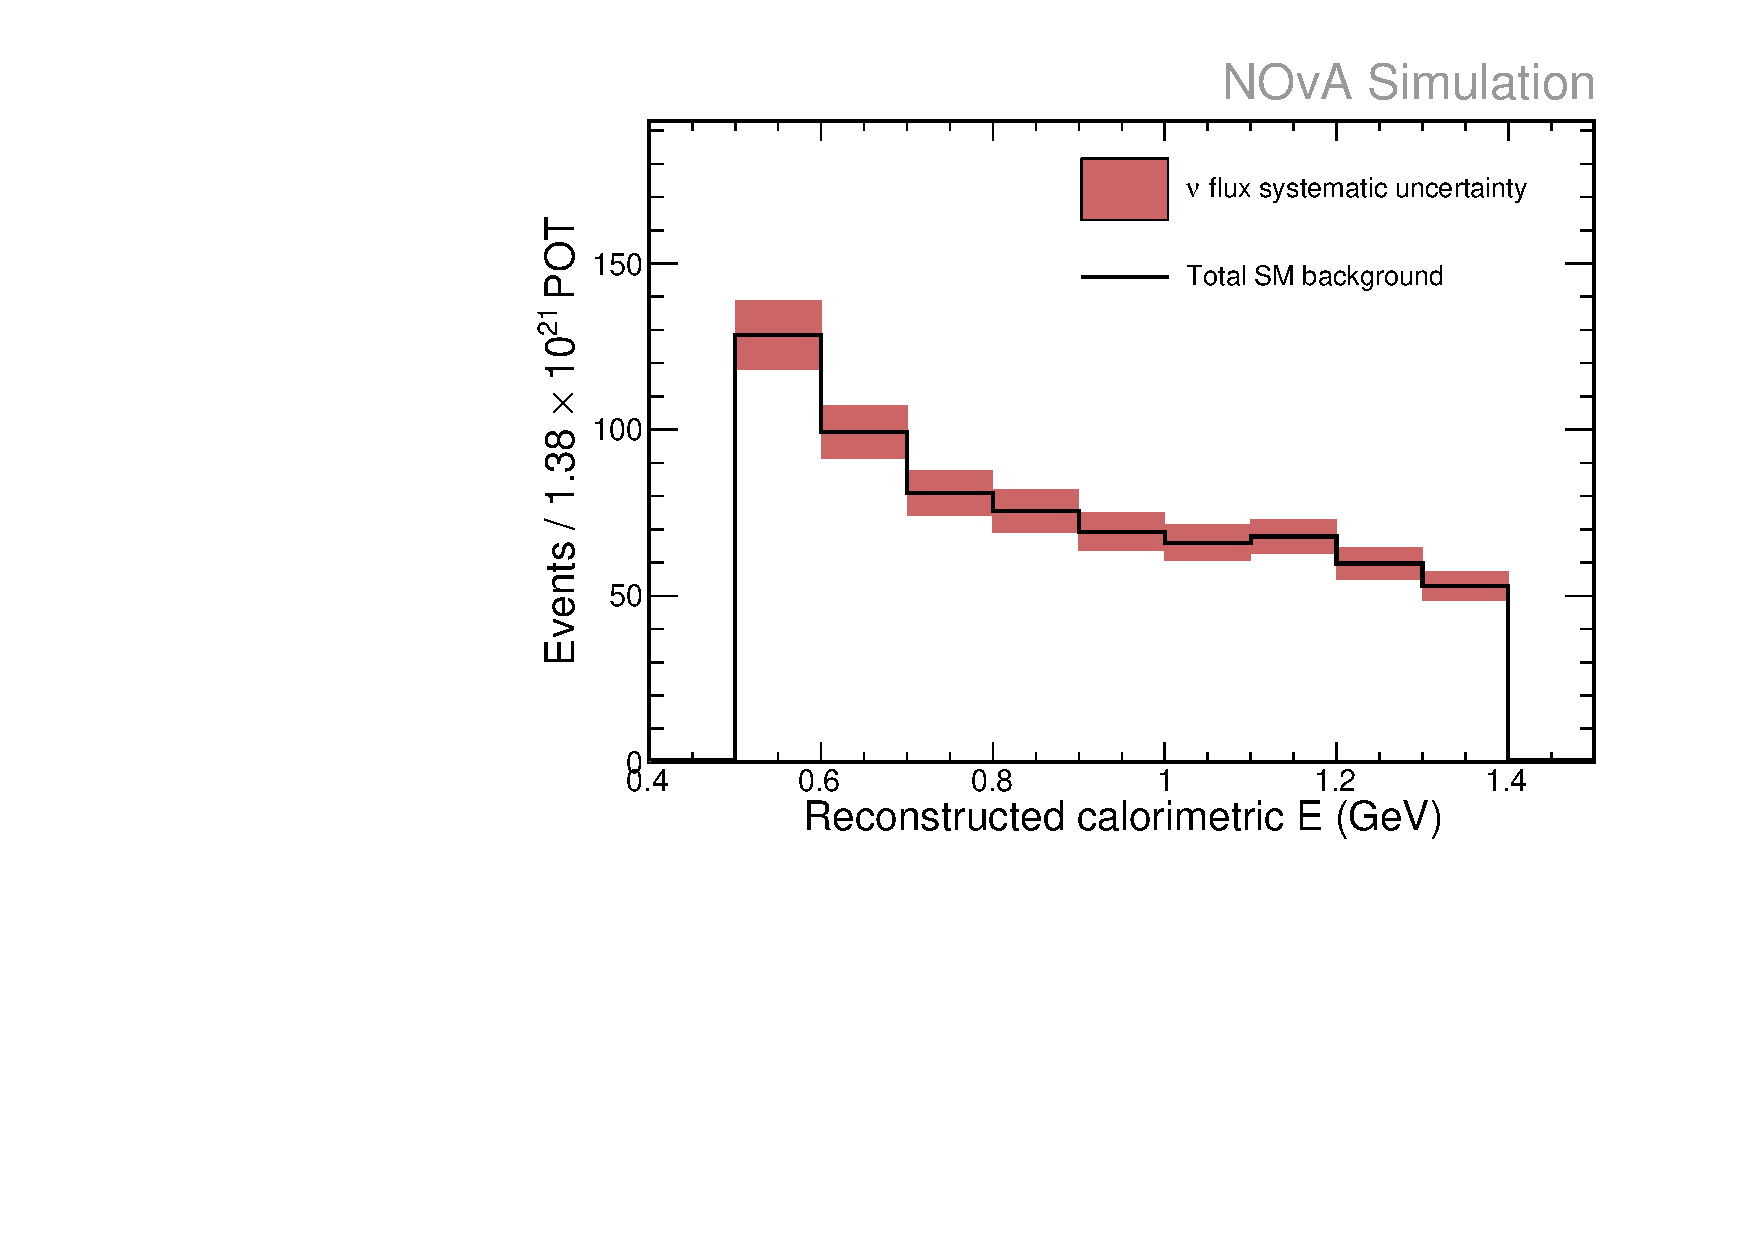
\includegraphics[width=.9\textwidth]{Plots/NuMM/SystShifts_beamSysts_Full_Graph.pdf}
\caption[Neutrino flux systematic uncertainty]{Effect of the total neutrino flux systematic uncertainty on the primary shower energy distribution of the \acrshort{SM} background events.}
\label{fig:NuMMFluxSysts}
\end{figure}

The effect of the total detector modelling and calibration systematic uncertainties on the number of \gls{SM} background events is asymmetrical, increasing the number of events by $+\unit[6.17]{\%}$ and decreasing by $\unit[3.69]{\%}$. The effect of these uncertainties dependents on the energy of the primary shower (which is the recoil electron for \gls{nuone} events), as can be seen in Fig.~\ref{fig:NuMMDetSysts}. This means that the energy distribution of the \gls{SM} background events can be significantly altered due to the detector uncertainties. The largest contribution comes from the absolute energy scale uncertainty, which has a one-sided effect of $\unit[+5.72]{\%}$. This is due to both the positive and the negative shift in the absolute energy scale increasing the total number of \gls{SM} background events. The light level and  Cherenkov systematic uncertainties are asymmetrical and alter the number of \gls{SM} background events in both directions by $^{+\unit[1.13]{\%}}_{\unit[-3.39]{\%}}$ and $^{\unit[+1.82]{\%}}_{\unit[-1.46]{\%}}$ respectively. The detector ageing and calibration shape systematic uncertainties are one sided by default and increase the number of the \gls{SM} background events by $\unit[+0.55]{\%}$ and $\unit[+0.69]{\%}$ respectively.

\begin{figure}[hbtp]
\centering
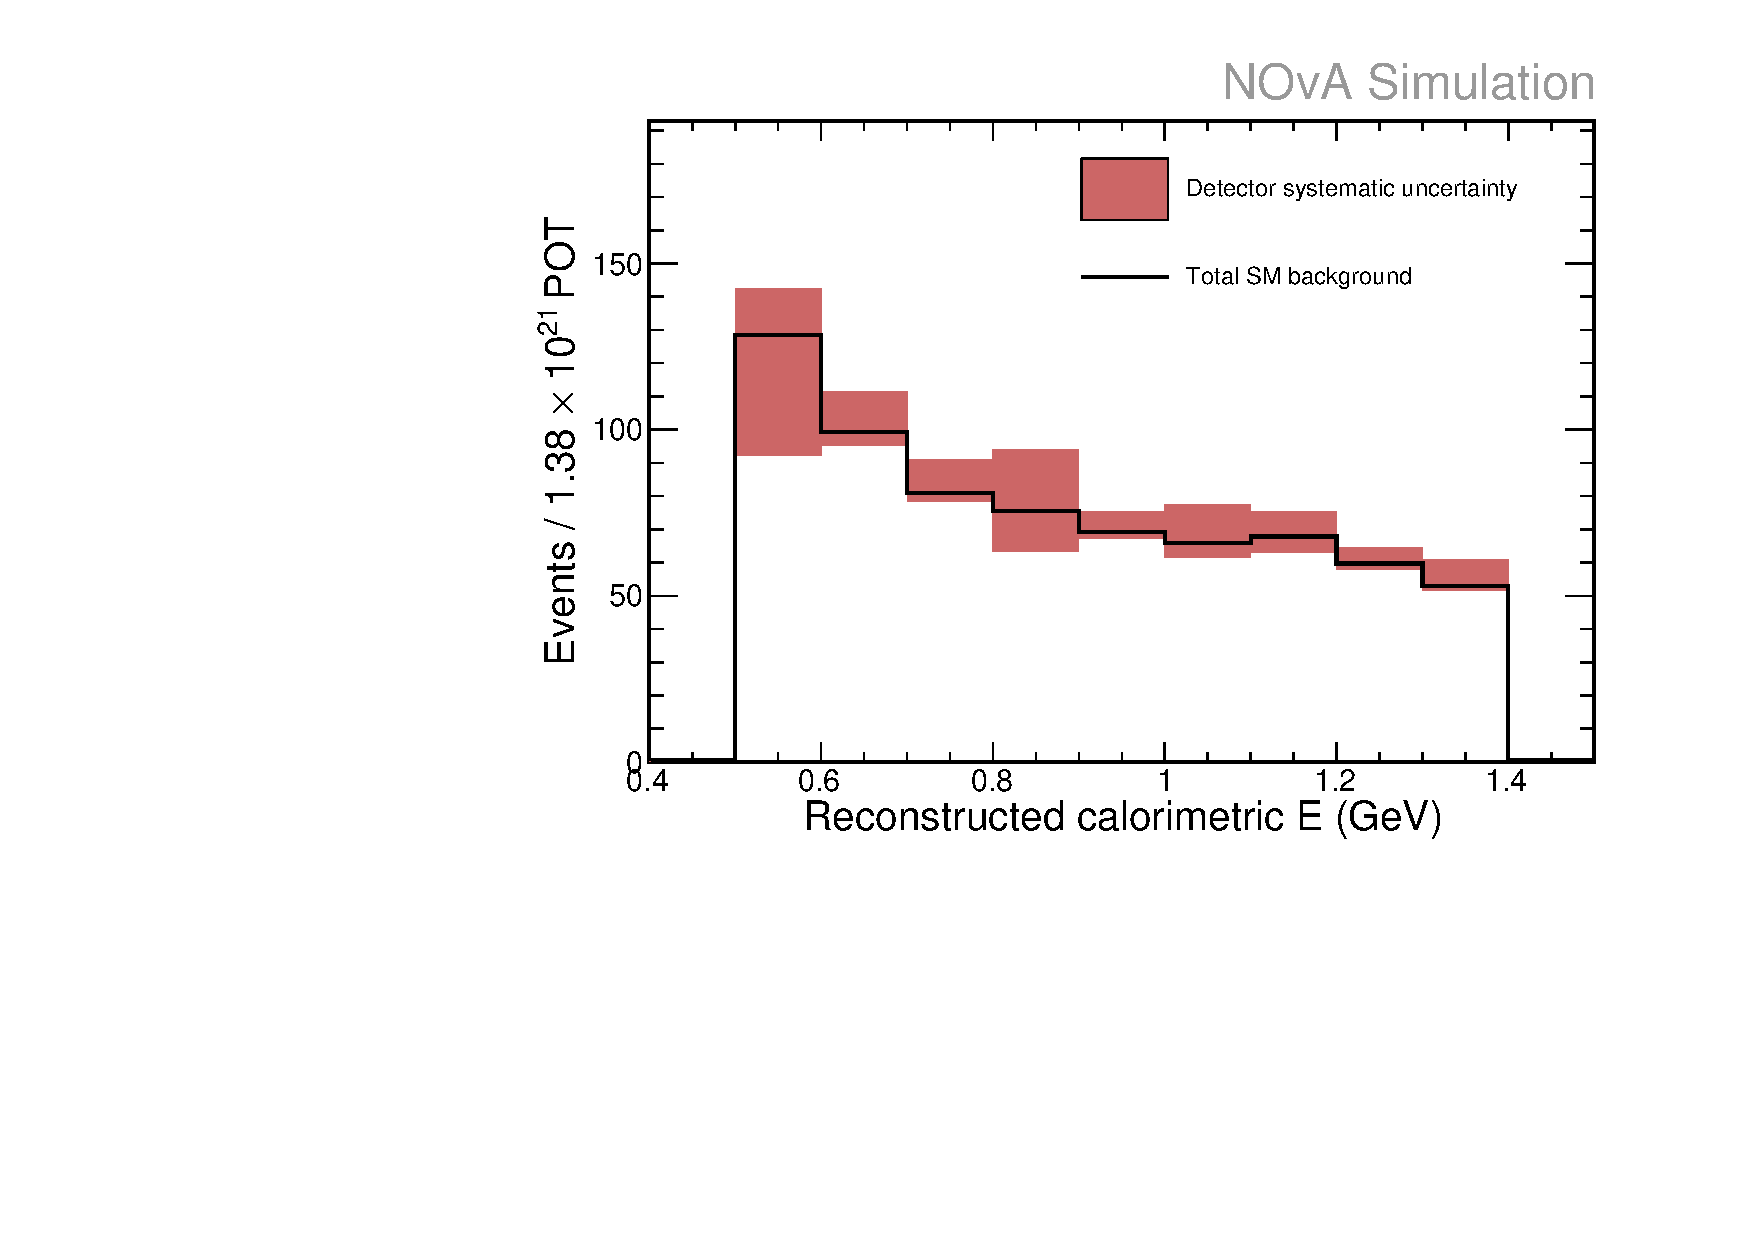
\includegraphics[width=.9\textwidth]{Plots/NuMM/SystShifts_detSysts_Full_Graph.pdf}
\caption[Detector systematic uncertainties]{Effect of the total detector systematic uncertainty on the primary shower energy distribution of the \acrshort{SM} background. The detector uncertainty consists of the absolute calibration, calibration shape, detector ageing, light level, and Cherenkov systematic uncertainties.}
\label{fig:NuMMDetSysts}
\end{figure}

Since we assume that the \gls{nuone} interaction is known precisely, the dominant \gls{nuone} component of the \gls{SM} background has no systematic uncertainty from neutrino interactions. Therefore, the neutrino interaction systematic uncertainty affects only the $181$ `Other background' events, which make up $\unit[34.9]{\%}$ of the total \gls{SM} background. Consequently, the total neutrino interaction uncertainty on the \gls{SM} background is relatively small, with a combined effect on the number of \gls{SM} background events of $^{+\unit[1.54]{\%}}_{-\unit[1.49]{\%}}$.
The most dominant neutrino interaction systematic uncertainties are related to interactions with $\pi^0$ in the final state,  such as the axial mass ($^{\unit[+0.97]{\%}}_{\unit[-0.90]{\%}}$) and the vector mass ($^{\unit[+0.41]{\%}}_{\unit[-0.35]{\%}}$) of the \gls{NC}\gls{Res} interactions, the scaling of the \gls{COHpi}\gls{NC} interactions ($^{\unit[+0.85]{\%}}_{\unit[-0.85]{\%}}$), or the mean free path of pions before they undergo an interaction ($^{\unit[+0.30]{\%}}_{\unit[-0.43]{\%}}$). Other neutrino interaction systematic uncertainties have only a marginal ($<\unit[0.3]{\%}$) effect on the number of \gls{SM} background events.

%The most dominant neutrino interaction systematic uncertainties are from the axial and vector masses of the \gls{NC}\gls{Res} interaction ($^{\unit[+0.97]{\%}}_{\unit[-0.90]{\%}}$ for axial and $^{\unit[+0.41]{\%}}_{\unit[-0.35]{\%}}$ for vector mass). Also significant is the effect of the coherent \gls{NC} scaling ($^{\unit[+0.85]{\%}}_{\unit[-0.85]{\%}}$), of the \gls{QE} normalization factor ($^{\unit[+0.31]{\%}}_{\unit[-0.24]{\%}}$), or of the mean free path of pions before they undergo an interaction ($^{\unit[+0.30]{\%}}_{\unit[-0.43]{\%}}$).


%Other uncertainties have only a very small impact. The ones that have an effect of $\left(>\pm\unit[0.1]{\%}\right)$ are the suppression of long-range nuclear effect and \gls{Res} events at low energy transfers, shape of the \gls{MEC} tuning dependent on the neutrino energy, single $\pi$ \gls{NC}\gls{DIS} production, distance parton travels before hadronization, axial mass of \gls{NC} elastic and \gls{CC}\gls{Res} interactions, branching ratios of radiative and $\eta$-resonance decays, or the $\pi$ angular distribution in the $\Delta$ resonance decays.

\iffalse
The largest systematic uncertainty for neutrino interaction comes from:
MaNCRES (0.97\%, -0.90\%) axial mass for NC resonant neutrino production $\pm\unit[20]{\%}$ - from GENIE,
MvNCRES (+0.41\%, -0.35\%) vector mass for NC resonant neutrino production $\pm\unit[10]{\%}$ - from GENIE,
COHNCScale208 (+0.85\%, -0.85\%),
ZNormCCQE (+0.31\%, -0.24\%) is the Z-expansion normalization and represents a $\unit[+20]{\%}/\unit[-15]{\%}$ QE normalization factor - GENIE,
hNFSI\_MFP\_2024 (+0.30\%, -0.43\%) the mean free path (mean distance traveled by) of pions before they undergo an interaction

Other notable $\left(>\pm\unit[0.1]{\%}\right)$ contributions are from (in no particular order)
RPAShapesupp2020 (how well is the RPA understood, this one suppresses it at low $Q^2$),
LowQ2RESSupp2020 (one sided uncertainty due to an observed discrepancy at low $Q^2$ of RES events in NOvA data),
MECShape2024Nu (neutrino energy dependence of the MEC fit), DISvpNC2pi\_2020 (normalization uncertainty for transition-DIS events, starting at $\unit[50]{\%}$ at high $W\leq\unit[3]{GeV}$ to $\unit[5]{\%}$ at $\unit[5]{GeV}$ - implemented individually for different number of $\pi$ and CC and NC),
DISvnNC1pi\_2020 (same as the previous one),
DISNuHadronQ1Syst, FormZone2024 (distance that a parton travels before hadronization),
MaNCEL (axial mass of NC elastic interactions $\pm\unit[25]{\%}$ - GENIE),
MaCCRES (axial mass for CC resonant interactions $\pm\unit[20]{\%}$ - GENIE),
RDecBR1gamma (branching ratio for radiative decays by $\pm\unit[50]{\%}$ - GENIE),
RDecBR1eta (tweaks the branching ratio of single $\eta$ decay by 50\% - the decay $R\rightarrow X+\eta$ - GENIE),
Theta_Delta2Npi (distorts the $\pi$ angular distribution in the decay $\Delta\rightarrow N+\pi$)
\fi

\iffalse
\begin{figure}[hbtp]
\centering
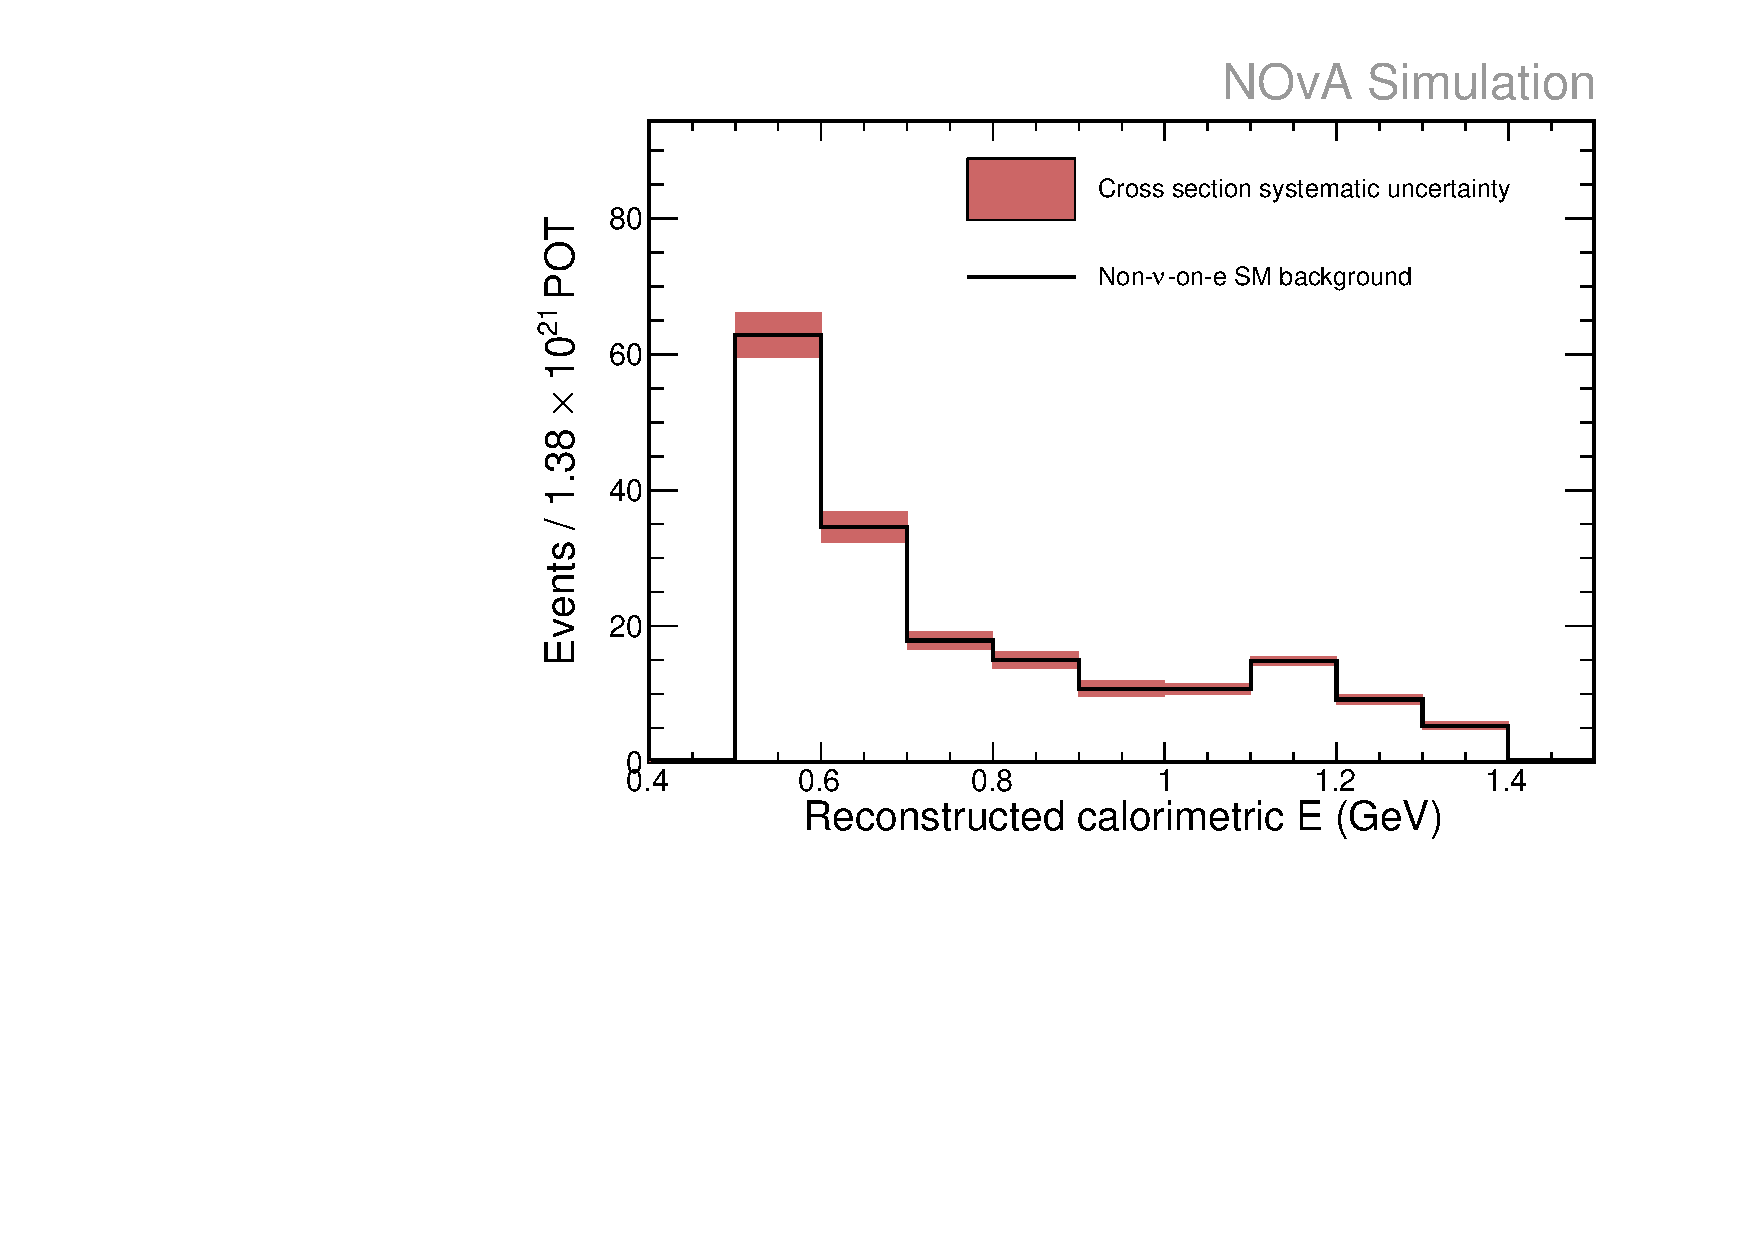
\includegraphics[width=.9\textwidth]{Plots/NuMM/SystShifts_xsecSysts_Full_Graph.pdf}
\caption[Neutrino cross section systematic uncertainty]{Effect of the neutrino cross section systematic uncertainty on the primary shower energy distribution of the non-\acrshort{nuone} part of the \acrshort{SM} background.}
\label{fig:NuMMXSecSysts}
\end{figure}
\fi

\section{Statistical analysis}\label{sec:NuMMStatisticalAnalysis}

% Likelihood
Our analysis compares the total observed number of events, $N_O$, with the expected (predicted) number of events, $N_E\left(\mu_\nu\right)$, which in general depends on the value of the effective neutrino magnetic moment, $\mu_\nu$, and is equal to the sum of the expected signal and background events:
\begin{equation}
N_E\left(\mu_\nu\right)=N_S\left(\mu_\nu\right)+N_B.
\end{equation}
The number of background events is equal to $N_{\gls{SM}}$ from Eq.~\ref{eq:NumberOfSMEventsWithSysts} and the number of signal events can be expressed as
\begin{equation}\label{eq:NuMMExpectedNumberOfSignalEvents}
N_S=56.80\times\left(\frac{\mu_\nu}{10^{-9}\mu_B}\right)^2,
\end{equation}
as described in Sec.~\ref{sec:NuMMEventSelection}.

The number of recorded events within a fixed time interval follows the Poisson distribution with the likelihood (probability) of observing $N_O$ events given a hypothesis predicting $N_E$ events defined as \cite{PDG.pdf}:
\begin{equation}\label{eq:Likelihood}
L\left(N_O;N_E\left(\mu_\nu\right)\right)=\frac{N_E\left(\mu_\nu\right)^{N_O}}{N_O!}e^{-N_E\left(\mu_\nu\right)}.
\end{equation}

%Log-likelihood ratio
To estimate and constrain $\mu_\nu$, we employ a frequentist approach using the Poisson-distributed likelihood ratio \cite{ExtendedMaximumLikelihood1990.pdf}
\begin{equation}
\lambda=\frac{L\left(N_O;N_E\left(\mu_\nu\right)\right)}{L_{sat}\left(N_O;N_O\right)}.
\end{equation}
Here, $L_{sat}$ is the so-called saturated model, for which $N_E=N_O$ and is constant with respect to $\mu_\nu$ \cite{PDG.pdf}. Maximising the likelihood with respect to $\mu_\nu$ is equivalent to minimising the \textit{`log-likelihood ratio'} described as:
\begin{align}\label{eq:LogLikelihoodStatsOnly}
-2\ln\lambda\left(\mu_\nu\right)&=
-2\ln\left(\frac{L\left(N_O;N_E\left(\mu_\nu\right)\right)}{L\left(N_O;N_O\right)}\right)\\
&=2\left[N_E\left(\mu_\nu\right)-N_O+N_O\ln\frac{N_O}{N_E\left(\mu_\nu\right)}\right].
\end{align}

According to Wilk's theorem \cite{WilksTheorem1938.pdf}, under the assumptions that the hypothesis is correct, the sample size is sufficiently large, and certain regularity conditions (which are met in our case) are satisfied, the log-likelihood ratio follows a chi-squared $\left(\chi^2\right)$ distribution. Therefore, the log-likelihood ratio serves not only to find the maximum likelihood estimators of $\mu_\nu$ but also to provide a statistic usable for a goodness-of-fit test \cite{PDG.pdf}.

%[wikipedia on Wilk's theorem] The model with more parameters (here alternative) will always fit at least as well — i.e., have the same or greater log-likelihood — than the model with fewer parameters (here null). Whether the fit is significantly better and should thus be preferred is determined by deriving how likely (p-value) it is to observe such a difference D by chance alone, if the model with fewer parameters were true. Where the null hypothesis represents a special case of the alternative hypothesis, the probability distribution of the test statistic is approximately a chi-squared distribution with degrees of freedom equal to df alt − df null respectively the number of free parameters of models alternative and null.

% Systematic uncertainties as nuisance parameters
\subsection{Treatment of systematic uncertainties}
%Including systematic uncertainties in the likelihood ratio
Systematic uncertainties are incorporated into the fitting framework as nuisance parameters that multiply the likelihood function in Eq.~\ref{eq:Likelihood}. Each systematic uncertainty is modelled according to the normal distribution centred at zero, with a standard deviation corresponding to its respective $1\sigma$ variation. Systematic uncertainties are treated as mutually uncorrelated, justifying their independent treatment.

Incorporating the nuisance parameters into the log-likelihood ratio function in Eq.~\ref{eq:LogLikelihoodStatsOnly} results in so-called \textit{`penalty terms'}. These terms are proportional to the square of each systematic pull's variation in units of $\sigma$, thereby increasing the log-likelihood ratio for solutions that favour non-zero systematic shifts:
\begin{equation}\label{eq:FullLogLikelihood}
-2\ln\lambda\left(\mu_\nu,\overrightarrow{\eta}\right)=-2\left[E\left(\mu_\nu,\overrightarrow{\eta}\right)-O+O\ln\frac{O}{O\left(\mu_\nu,\overrightarrow{\eta}\right)}\right] + \sum_{i=1}^{M}\left(\frac{\eta_i}{\sigma}\right)^2.
\end{equation}
Here, $\overrightarrow{\eta}$ is a vector of $M$ nuisance parameters representing the effect of systematic uncertainties.

In practice, we produce systematically shifted predictions for each systematic uncertainty with shifts at fixed integer $\sigma$ values. Due to the computationally expensive nature of reproducing the detector simulation, variations in detector and calibration systematic uncertainties are estimated only at $\pm 1\sigma$ values. However, for beam and cross section uncertainties, variations are estimated at $\pm 1\sigma$, $\pm 2\sigma$, and $\pm 3\sigma$ levels. These systematically shifted predictions are then interpolated using cubic spline-based fit. For one-sided systematic uncertainties, such as detector ageing and calibration shape uncertainties, the fit is fixed at zero for the excluded side \cite{NitishOscMeasuremetPCAStatisticalAna2021.pdf}.

%[Nitish's thesis] The best-fit oscillation parameters are derived by minimizing this equation with respect to these parameters and is done using a MIGRAD based algorithm [125]. The parametrisation is derived by defining the variation in the prediction at specific $\sigma$ values, for example: $-2,-1,0,+1,+2 \sigma$ and interpolating the deviations in each analysis bin using a cubic spline-based method. This is sufficiently general for all the systematics considered in the analysis, including those with non-Gaussian uncertainties. For one-sided systematic shifts the interpolation parametrizes the overall deviation by fitting a flat line at 0 for the excluded shifts and only uses the included shifts.

%[Nitish's thesis] pg 156: As mentioned before, the nuisance parameters in the likelihood fit are derived by interpolating between shifts at given numerical sigma values for the above uncertainties for each analysis bin.

\iffalse
[Nitish's thesis]
This prediction is fit to the NuMI data using the traditional Poisson log-likelihood for binned spectra \cite{ExtendedMaximumLikelihood1990.pdf}. This is given as:
\begin{equation}
-2\ln\lambda\left(\theta,\overrightarrow{\eta}\right)=-2\sum_{i=1}^{N}\left[\mu_i\left(\theta,\overrightarrow{\eta}\right)-n_i+n_i\ln\frac{n_i}{\mu_i\left(\theta,\overrightarrow{\eta}\right)}\right] + \sum_{k=1}^M \eta_k^2,
\end{equation}
where $\mu_i$ denotes the predicted number of events in each analysis bin $i$ as a function of the neutrino magnetic moment $\theta$ and the nuisance parameters $\eta$, which for us are the systematic shifts. $n_i$ is the observed number of events in that bin. The last term denotes the penalty given to favouring a non-zero systematic variation for M set of systematic uncertainties. The best-fit oscillation parameters are derived by minimizing this equation with respect to these parameters and is done using a MIGRAD based algorithm [125]. The likelihood takes into account the Poisson deviations of the prediction from data in each analysis bin (given by the ln term) as well as an overall Poisson fluctuation on the total number of predicted events. ...the penalty is calculated for the amount of $\sigma$ deviation favoured in the fit, i.e if the fit favours a $1.2\sigma$ deviation from the central value prediction then the penalty to $-2\ln\lambda$ is given by $1.2^2=1.44$. The parametrisation is derived by defining the variation in the prediction at specific $\sigma$ values, for example: $-2,-1,0,+1,+2 \sigma$ and interpolating the deviations in each analysis bin using a cubic spline-based method. This is sufficiently general for all the systematics considered in the analysis, including those with non-Gaussian uncertainties. For one-sided systematic shifts the interpolation parametrizes the overall deviation by fitting a flat line at 0 for the excluded shifts and only uses the included shifts.
%[125] is R. Brun et al. TMinuit Class Reference. ROOT Documentation.
\fi

%Null hypothesis
\subsection{Hypothesis testing and confidence limits}\label{sec:HypothesisTesting}

%Given the number of observed events we want to test whether we can describe the number of observed events only using the \gls{SM} prediction, or if we need a neutrino magnetic moment as well. To do this we test the null hypothesis, which states that the number of observed selected events is only due to the \gls{SM}. 

To evaluate whether the observed number of events can be described solely using the \gls{SM} prediction, we perform a hypothesis test for the \textit{`null hypothesis'}, $H_0$, for which $\mu_\nu=0$, $E_S=0$, and hence the expected number of events is $N_E=N_B$. The log-likelihood ratio is in this case
\begin{equation}\label{eq:NullHypothesisLogLikelihood}
-2\ln\lambda_{H_0}=
2\left[N_B-N_O+N_O\ln\frac{N_O}{N_B}\right] + \sum_{k=1}^M \eta_k^2
\end{equation}
and its minimum follows a $\chi^2$ distribution with one degree of freedom. This allows us to calculate the p-value of the goodness-of-fit of the null hypothesis. We reject the null hypothesis if the statistical test yields a p-value below a critical value - significance level. We set the significance level at $\alpha=0.10$, which is a common threshold in other measurements of the neutrino magnetic moment, as discussed in the introduction to this chapter.

%We want to test the null hypothesis, which states that there is no neutrino magnetic moment and all the observed events are due to the \gls{SM} - $\mu=0$. If we reject the null hypothesis, we want to estimate the size of the neutrino magnetic moment, and if we fail to reject the null hypothesis, we want to place a limit on the size of the neutrino magnetic moment. For all these, we are using the likelihood ratio test statistics. The likelihood ratio test statistics is a ratio of the likelihood (probability) to observe the data given some hypothesis $H\left(\mu\right)$, over the likelihood of the "alternate" hypothesis under the best fit point.

If we fail to reject the null hypothesis, defined as $p>\alpha$, we establish an upper limit on the value of the effective muon neutrino magnetic moment. We consider our results to represent only the $\nu_\mu$ thanks their high purity in our neutrino beam, as described in Sec.~\ref{sec:NuMI}.

The upper limit is calculated by iterating over a fixed range of neutrino magnetic moment values and calculating the minimum log likelihood from Eq.~\ref{eq:FullLogLikelihood} at each iteration, while profiling over the nuisance parameters (systematic variations). This means that at each iteration, the value of the neutrino magnetic moment is fixed, and the log-likelihood function is minimised with respect to the systematic shifts. The minimisation of the log-likelihood ratio in  is done using a MIGRAD-based algorithm in ROOT \cite{ROOT}.

The minimum of the log-likelihood, as a function of the neutrino magnetic moment, follows a $\chi^2$ distribution with one degree of freedom and is often denoted as
\begin{equation}
-2\ln\lambda\left(\theta,\hat{\overrightarrow{\eta}}\right)\equiv \Delta\chi^2\left(\mu_\nu\right).
\end{equation}
Here $\hat{\overrightarrow{\eta}}$ denotes the vector of systematic shifts that minimise the log-likelihood for that specific $\mu_\nu$. We determine the $90\%$ \gls{CL} limit on the neutrino magnetic moment (equal to $1-\alpha$) as the range of $\mu_\nu$ values for which 
\begin{equation}
\Delta\chi^2<2.71.
\end{equation}
This is calculated as the integral of the right tail of the $\chi^2$ distribution with one degree of freedom.

%%%%%%%%%%%%%%%%%%%%%%%%%%%%%%%%%%%%%%%%%%%%%%%%%%%%%%%%%%%%%%%%%%%%%
%%%                             RESULTS                           %%%
%%%%%%%%%%%%%%%%%%%%%%%%%%%%%%%%%%%%%%%%%%%%%%%%%%%%%%%%%%%%%%%%%%%%%
\section{Results}\label{sec:NuMMResults}
To avoid biasing our decisions based on the number and distribution of the observed data events, we performed the event selection, studied systematic uncertainties, and decided on the statistical analysis methods prior to revealing the data samples in a so-called blinded analysis. We first validated the selected analysis methods using fake data, which were generated by applying a random fluctuation to the predicted number of events based on the Poisson distribution.

After investigating results from the fake data studies we unblinded the data sample and obtained the total number of observed events passing our selection. The number of selected events recorded in the \gls{NOvA} \gls{ND} corresponding to exposure $1.38\times 10^{21}$~\acrshort{POT} is
\begin{equation}
N_O = 773.
\end{equation}

Since we are only comparing the total number of predicted and observed events, the \gls{BF} point for the number of signal events can be simply calculated as
\begin{equation}
N_{S,\acrshort{BF}}= N_O-N_B = 72.67.
\end{equation}

From Eq.~\ref{eq:NuMMExpectedNumberOfSignalEvents} we get the \gls{BF} for the neutrino magnetic moment as
\begin{equation}
\mu_{\nu_\mu,\acrshort{BF}} = \sqrt{\frac{72.67}{56.80}} \times 10^{-9}\mu_B = 1.13\times 10^{-9}\mu_B.
\end{equation}

%Distribution of events
The final distribution of the predicted \gls{SM} background events, predicted signal events corresponding to $\mu_{\nu}=10^{-9}\mu_B$, and the observed data events as a function of the primary shower's reconstructed calorimetric energy is shown in Fig.~\ref{fig:NuMMResults_Distribution}. We do not use this energy distribution of events for hypothesis testing or parameter estimation, only to validate whether our simulation predicts the observation with sufficient precision. As can be seen, the observed data are within the systematic and statistical uncertainty for all the displayed bins with the only exception being the bin between $\left(\unit[0.9]{GeV},\unit[1.0]{GeV}\right)$. The discrepancy between data and simulation in this bin is however still within two standard variations from the accepted values and therefore we conclude that the simulation predicts the observed data satisfyingly well.

\begin{figure}[hbtp]
\centering
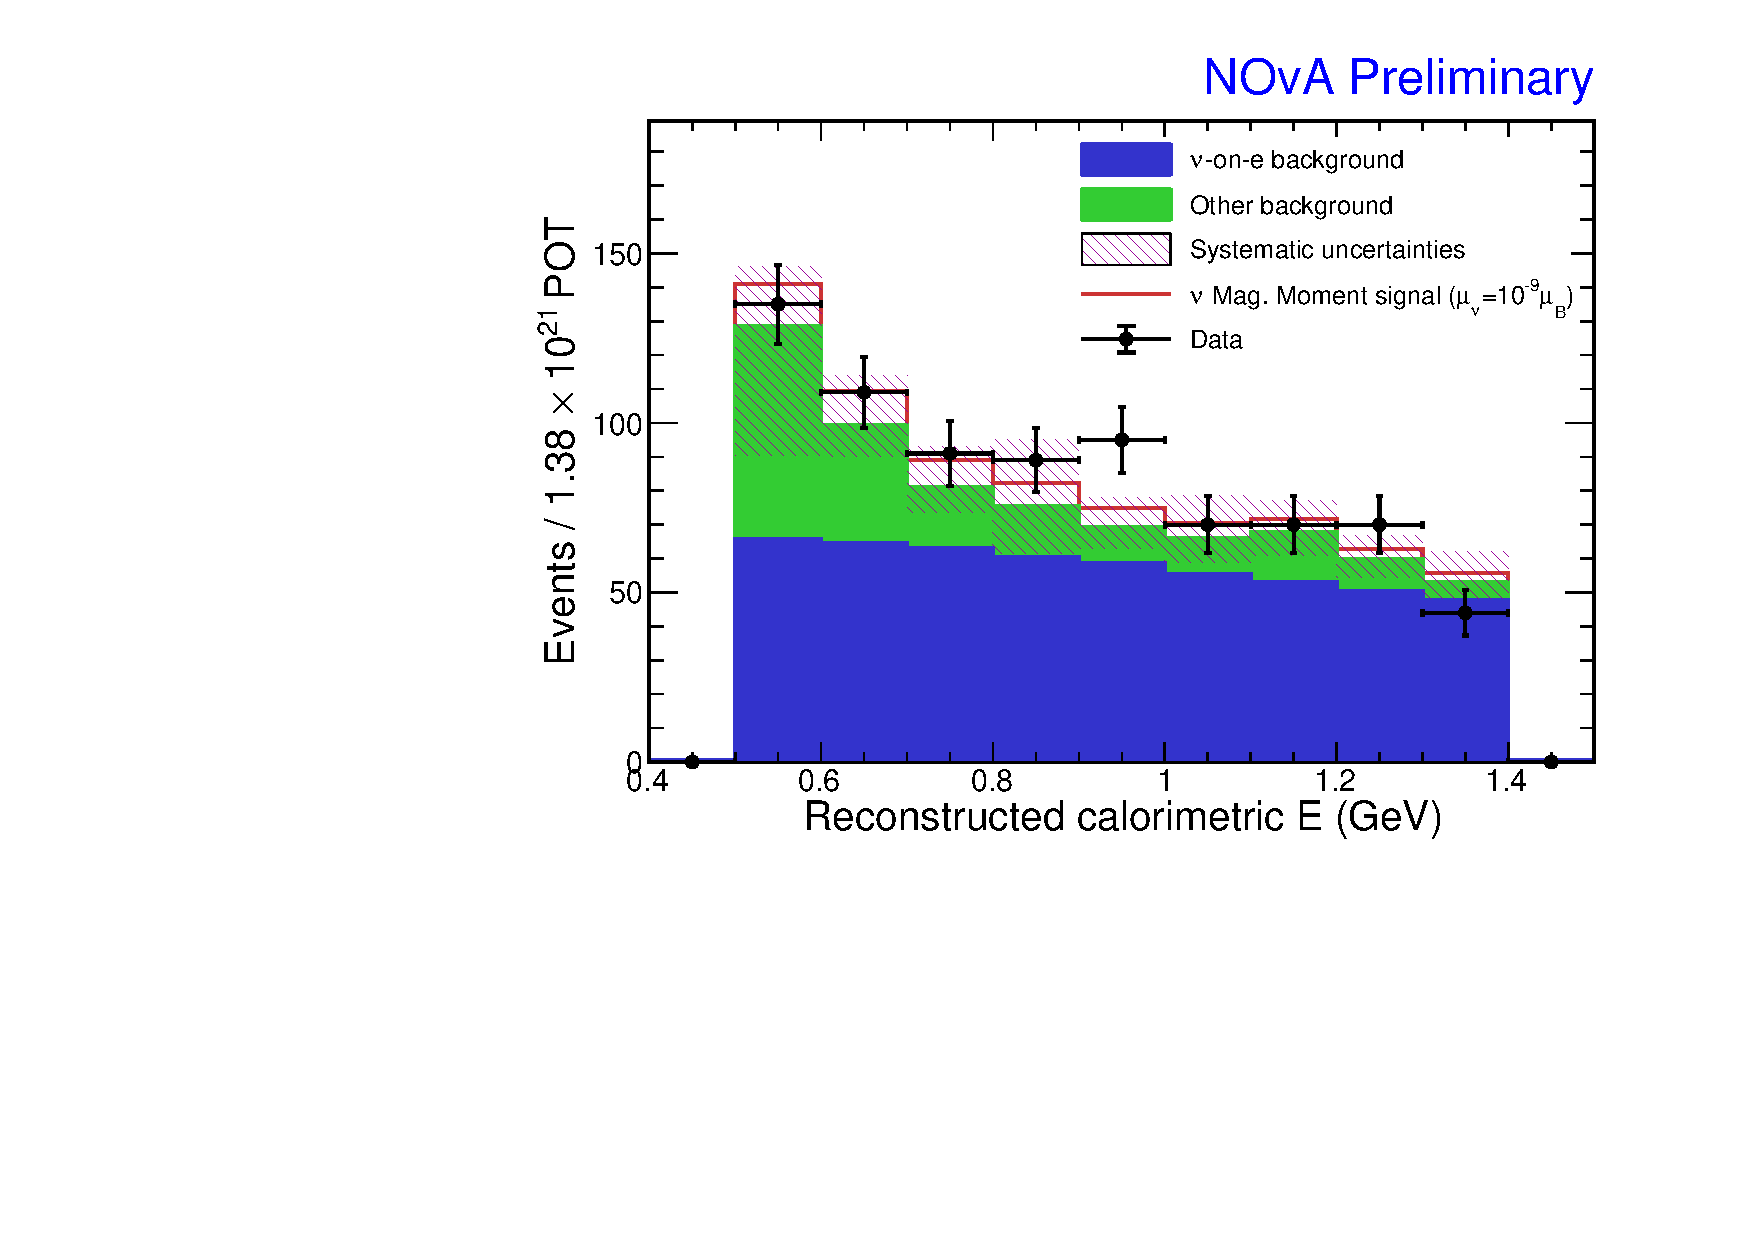
\includegraphics[width=\textwidth]{Plots/NuMM/Stacked.pdf}
\caption[Final prediction and data comparison]{Comparison of the observed data to the prediction of the neutrino magnetic moment signal corresponding to $\mu_\nu=10^{-9}\mu_B$ (red line) and the \acrshort{SM} background (filled area) as a function of the reconstructed calorimetric energy of the most energetic shower. The \acrshort{SM} background is divided into the \acrshort{nuone} component in blue and the rest in green, with the associated systematic uncertainty on the \acrshort{SM} background shown in shaded purple. Data is shown with statistical uncertainty based on Poisson distribution. All samples are scaled to the true data exposure $1.38\times 10^{21}$ \acrshort{POT}.}
\label{fig:NuMMResults_Distribution}
\end{figure}

% Need to describe / cite where did I get the p value from - is there a function in ROOT
% Also need to describe the minimization mechanism - is this minuit or migrad or are they the same thing?

%%% Results of the hypothesis test
We calculated the minimum log likelihood for the null hypothesis, as described in Eq.~\ref{eq:NullHypothesisLogLikelihood}, as 
\begin{equation}
-2\ln\lambda_{H_0,min}=1.02964,
\end{equation}
which corresponds to the double sided p-value of $0.31$. Since this value is larger than our pre-determined significance level of $0.1$, we are not able to reject the null hypothesis. This means that we did not observe an excess of \gls{nuone} events above the \gls{SM} background.

As described in Sec.~\ref{sec:HypothesisTesting}, we can determine the limit on the value of the effective muon neutrino magnetic moment by calculating $\Delta\chi^2$ for a range of $\mu_\nu$ value as shown in Fig.~\ref{fig:NuMMResults_ChisqLimit}. From this distribution we calculate the limit as
\begin{equation}\label{eq:NuMMLimit}
\mu_{\nu_\mu}<1.91\times10^{-9}\mu_B\,\,\,\textsf{at}\,\,\,90\%\, \gls{CL}.
\end{equation} 

We can also estimate the systematic uncertainty on the best fit point from the $\Delta\chi^2$ distribution shown in  Fig.~\ref{fig:NuMMResults_ChisqLimit} by taking the $1\sigma$ range $\left(\Delta\chi^2=1\right)$ of the full systematic uncertainty distribution. The $1\sigma$ range for all systematics is $\left(0.14,1.63\right)\times 10^{-9}\mu_B$, which is equivalent to the best fit point having an uncertainty:
\begin{equation}
\mu_{\nu_\mu,\acrshort{BF}}=\left(1.13^{+0.50}_{-0.99}\right)\times 10^{-9}\mu_B.
\end{equation}

\begin{figure}[hbtp]
\centering
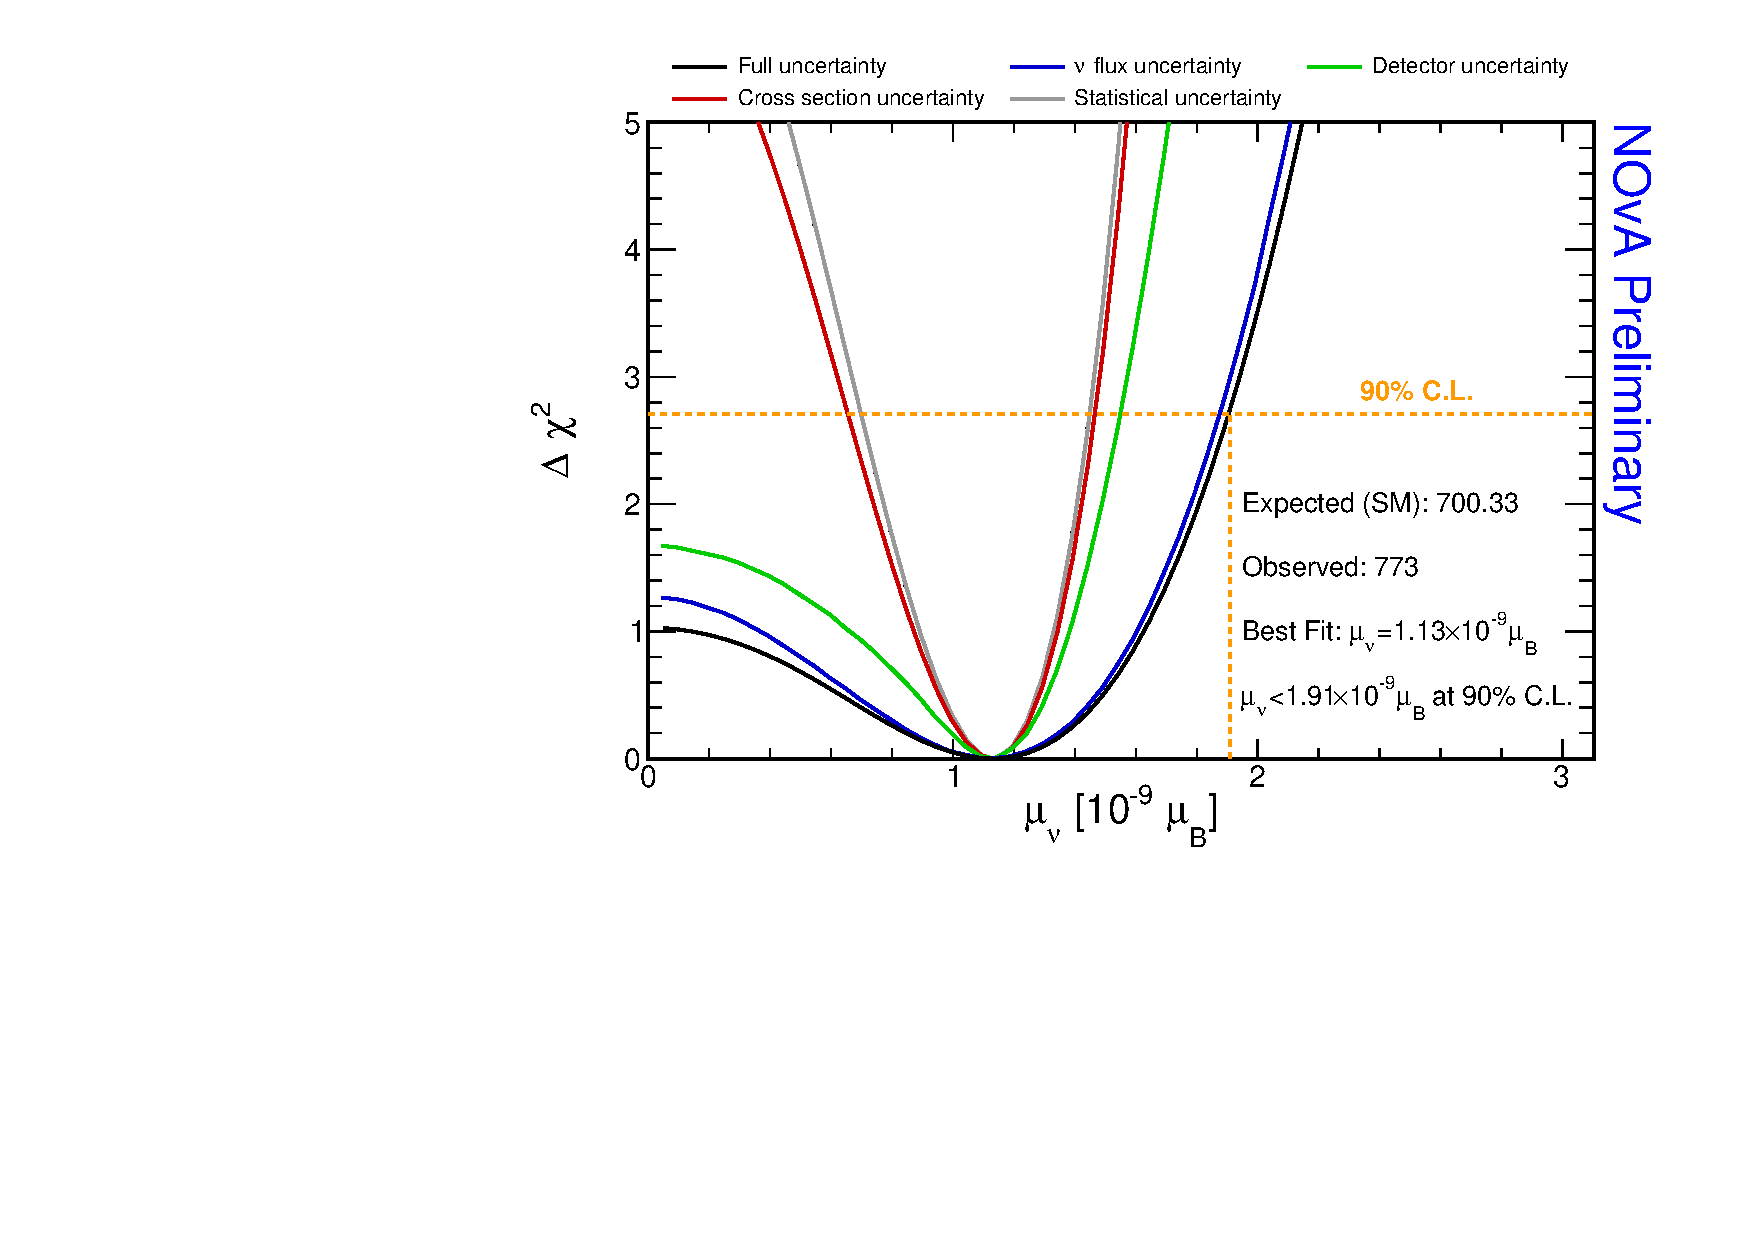
\includegraphics[width=\textwidth]{Plots/NuMM/NuMMLimit_FinalMoneyPlot.pdf}
\caption[Distribution of the minimum log likelihood ratio as a function of the neutrino magnetic moment]{Distribution of the minimum log likelihood ratio, equal to $\Delta\chi^2$, as a function of the neutrino magnetic moment as determined from a fit of the prediction to the observed data. The minimum is calculated by profiling over systematic uncertainties, as explained in text. Various selections of systematic uncertainties included in the fit are shown, with no systematic uncertainties included in gray (statistics-only result), neutrino flux, detector, and neutrino cross section systematic uncertainties in blue, green, and green respectively. The black line shows the distribution with the full range of systematic uncertainties included in the fit. This distribution is used to determine the $90\%$\gls{CL} limit on the value of the effective muon neutrino magnetic moment, by calculating the value corresponding to $\Delta\chi^2=2.71$, as described in text.}
\label{fig:NuMMResults_ChisqLimit}
\end{figure}

% Uncertainty on the best fit point
%[NOvAResultsNuOnly2018.pdf] TABLE VI. Sources of uncertainty and their estimated average impact on the oscillation parameters in the joint fit. This impact is quantified using the increase in the one-dimensional 68\% C.L. interval, relative to the size of the interval when only statistical uncertainty is included in the fit. 

%[Nitish's thesis]pg 156: As mentioned before, the nuisance parameters in the likelihood fit are derived by interpolating between shifts at given numerical sigma values for the above uncertainties for each analysis bin. One can then evaluate the size of the uncertainties in many ways. For the appearance channel, one can compare different systematics based on the effect it has on the total number of predicted signal and background events when varied by $\pm1\sigma$, as shown in Fig. 4.12. One can also estimate its effect by fitting to Asimov data using the central value prediction and varying the MC expectation based on the systematic variation. This takes the form of the effect of the systematic on the individual oscillation parameters [79], as shown in Figs. 4.13 and 4.14. All of these metrics show that the analysis is statistically limited, i.e the systematic error is smaller than the statistical error in the prediction. \cite{NitishOscMeasuremetPCAStatisticalAna2021.pdf}

%%%%%%%%%%%%%%%%%%%%%%%%%%%%%%%%%%%%%%%%%%%%%%%%%%%%%%%%%%%%%%%%%%%%%
%%%                            CONCLUSION                         %%%
%%%%%%%%%%%%%%%%%%%%%%%%%%%%%%%%%%%%%%%%%%%%%%%%%%%%%%%%%%%%%%%%%%%%%
\section{Summary}\label{sec:NuMMConclusion}

We analysed a selection of events recorded in the \gls{NOvA} \gls{ND}, searching for an excess of \gls{nuone} interactions over the \gls{SM} background, which would indicate the presence of an effective muon neutrino magnetic moment. In total, we observed 773 events, compared to the predicted 700.33 \gls{SM} background events. This resulted to a \gls{BF} value for the effective muon neutrino magnetic moment of $\mu_{\nu_\mu,\acrshort{BF}}=\left(1.13^{+0.50}_{-0.99}\right)\times 10^{-9}\mu_B$. However, we failed to reject the null hypothesis, which states that the observed events can be fully described by the \gls{SM}, and conclude that no excess of \gls{nuone} events was found. Consequently, we placed an upper limit on the effective muon neutrino magnetic moment of $\mu_{\nu_\mu}<19.1\times10^{-10}\mu_B$ at $90\%$ \gls{CL}.
%Maybe also mention that I've only done a counting experiment and that my selection involved selecting events between 0.5-1.4 GeV
%Also I need to mention the exposure and the data taking time in here

%Discuss the effect of statistical and systematic uncertainties
The uncertainty on the background prediction is dominated by systematic uncertainty on the neutrino flux prediction, as shown in Fig.~\ref{fig:NuMMResults_ChisqLimit}. Detector-related uncertainties represent the second largest contribution, while neutrino interaction uncertainties are sub-dominant. Additionally, the low neutrino magnetic moment cross-section leads to significant statistical uncertainty on the result, as the number of neutrino magnetic moment signal events corresponding to the current best limits is significantly smaller than our predicted \gls{SM} background.

By comparing our result to results from other experiments \cite{PDG.pdf}, shown in the introduction of this chapter, we can conclude that our $90\%$ \gls{CL} limit is less stringent than the current world-leading limit for muon neutrinos of $\mu_{\nu_\mu}<6.8\times 10^{-10}\mu_B$  at $\unit[90]{\%}$ \gls{CL} \cite{LSNDLimits2001.pdf}. It is also less strict than the previous \gls{NOvA} limit of $\mu_{\nu_\mu}<15.8\times 10^{-10}\mu_B$ at $\unit[90]{\%}$ \gls{CL} \cite{nuMM-thesis-biaow.pdf}, which however does not account for the effect of systematic uncertainties, making direct comparison difficult. The reason for failing to improve upon the first \gls{NOvA} result is a more careful consideration of backgrounds and systematic uncertainties, which loosened the significance of our result.

%Improvements in statistics, adding RHC data and more data to follow
There are several opportunities for improvement in future iterations of this analysis. The most straightforward enhancement is increasing the sample size, as \gls{NOvA} is expected to continue running through 2026, which will more than double the available \gls{FHC} data. Additionally, incorporating \gls{RHC} data, either combined with the \gls{FHC} data or through a separate analysis, could extend the reach of the study. It may also help disentangle the impact of some of the backgrounds and systematic uncertainties, as the neutrino magnetic moment affects neutrinos and antineutrinos equally, while the backgrounds may vary between them.

% Improved reconstruction, simulation and calibration - Test Beam plug
Further improvements can be achieved through enhancements in detector simulation, calibration, and event reconstruction, particularly for single-electron events. Ongoing analysis of data from the \gls{NOvA} Test Beam detector, as discussed in Chapter~\ref{sec:TestBeamCalibration}, will be instrumental in reducing the effect of detector-related systematic uncertainties. Additionally, implementing new hadron production data from the NA61 and EMPHATIC experiments will significantly improve the neutrino flux prediction and reduce the associated systematic uncertainties, as explained in Sec.~\ref{sec:NOvASimulation}.

%Improved event selection - going below 0.5 GeV, creating control samples
Another place for improvement lies in refining the event selection, either by increasing the signal-to-background ratio through cut optimisation, or by introducing one or more control samples. Control samples, which are regions dominated by specific background with minimal signal events, can be fitted alongside the signal region to help constrain background levels and their associated systematic uncertainties.

In the signal sample, we applied a low energy cut at $\unit[0.5]{GeV}$ due to time constraints in investigating low-energy backgrounds and corresponding systematic uncertainties. In the future, it may be possible to lower this energy cut, thereby improving the signal-to-background ratio. However, as can be seen in Fig.~\ref{fig:NuMMBackgroundDecomposition}, there are significant backgrounds at low energies with a similar shape to signal, making it essential to properly study these backgrounds before lowering the energy threshold.

%Improving the fitting - doing an energy dependent fit
Another potential improvement involves transitioning from a single-bin fit to a multi-bin fit, using the reconstructed calorimetric energy of the leading shower. The \gls{NOvA} \gls{LDM} analysis \cite{NOVA-doc-59439} employs a template fitting approach, which assumes that the prediction accurately describes the shapes of the signal and background distributions, while allowing their normalisations to vary freely. This method reduces the number of free parameters in the fit while enhancing sensitivity to the shape differences between the signal and background. This is particularly relevant for our analysis, as the neutrino magnetic moment signal rises sharply at lower electron recoil energies, while the dominant \gls{nuone} background follows a more uniform distribution. On the other hand, this technique assumes no prior knowledge on the normalisation. A combined approach using both template-fitting and normalisation constraints might offer the optimal solution.

%Future in DUNE
%For the energy deposition of electron in LArTPC might be a good source this https://iopscience.iop.org/article/10.1088/1748-0221/15/03/P03022/pdf
